\documentclass[12pt, twoside]{../style-files/uosthesis}

\usepackage{amssymb}
\usepackage{titlesec}
\usepackage{amsmath}
\usepackage{float}
\usepackage{graphicx}
\usepackage{caption}
\usepackage{subfig}
\usepackage{graphicx}
\usepackage{xcolor}
\usepackage[round]{natbib}
\usepackage[section]{placeins}
\usepackage{mathrsfs}
\usepackage{bm}
\usepackage{stmaryrd}
\usepackage[utf8]{inputenc}
\usepackage{siunitx}
\usepackage{combelow}
\usepackage{afterpage}
\usepackage{epigraph}
\usepackage[titletoc]{appendix}

\usepackage{tikz}
\usetikzlibrary{fadings}
\usetikzlibrary{snakes}
\usetikzlibrary{decorations.markings}
\usetikzlibrary{decorations.pathmorphing}
\usetikzlibrary{arrows,shapes, positioning}
\usepackage{booktabs}
\usepackage{multirow}
\usepackage{rotating}
\usepackage{tabularx}
\usepackage{makecell}

%%%%%%%%%%%%%%%%%%%%%%%%%%%%%%%%%%%%%%%%%%%%%%%%%%%%%%%%%%
% the following is to alter tikz settings to improve springs figure.
\usetikzlibrary{decorations.pathmorphing,calc,patterns}
\makeatletter
\def\pgfdecorationspringstraightlinelength{0.5cm}
\def\pgfdecorationspringnumberofelement{8}
\def\pgfdecorationspringnaturallength{5cm}
\pgfkeys{%
	/pgf/decoration/.cd,
	spring straight line length/.code={%
		\pgfmathsetlengthmacro\pgfdecorationspringstraightlinelength{#1}},
	spring natural length/.code={%
		\pgfmathsetlengthmacro\pgfdecorationspringnaturallength{#1}},
	spring number of element/.store in=\pgfdecorationspringnumberofelement
}

\pgfdeclaredecoration{coil spring}{straight line}{%
	\state{straight line}[%
	persistent precomputation = {%
		% Compute the effective length of the spring (without the length
		% of the two straight lines): \pgfdecorationspringeffectivelength
		\pgfmathsetlengthmacro{\pgfdecorationspringeffectivelength}%
		{\pgfdecoratedpathlength-2*\pgfdecorationspringstraightlinelength}
		% Compute the effective length of one coil pattern:
		% \pgfdecorationspringeffectivelengthofonecoil
		\pgfmathsetlengthmacro{\pgfdecorationspringeffectivelengthofonecoil}%
		{\pgfdecorationspringeffectivelength/\pgfdecorationspringnumberofelement}
	},
	width = \pgfdecorationspringstraightlinelength,
	next state = draw spring]{%
		\pgfpathlineto{%
			\pgfqpoint{%
				\pgfdecorationspringstraightlinelength}{0pt}}
	}
	\state{draw spring}%
	[width=\pgfdecorationspringeffectivelengthofonecoil,
	repeat state=\pgfdecorationspringnumberofelement-1,next state=final]{%
		\pgfpathcurveto
		{\pgfpoint@onspringcoil{0    }{ 0.555}{1}}
		{\pgfpoint@onspringcoil{0.445}{ 1    }{2}}
		{\pgfpoint@onspringcoil{1    }{ 1    }{3}}
		\pgfpathcurveto
		{\pgfpoint@onspringcoil{1.555}{ 1    }{4}}
		{\pgfpoint@onspringcoil{2    }{ 0.555}{5}}
		{\pgfpoint@onspringcoil{2    }{ 0    }{6}}
		\pgfpathcurveto
		{\pgfpoint@onspringcoil{2    }{-0.555}{7}}
		{\pgfpoint@onspringcoil{1.555}{-1    }{8}}
		{\pgfpoint@onspringcoil{1    }{-1    }{9}}
		\pgfpathcurveto
		{\pgfpoint@onspringcoil{0.445}{-1    }{10}}
		{\pgfpoint@onspringcoil{0    }{-0.555}{11}}
		{\pgfpoint@onspringcoil{0    }{ 0    }{12}}
	}
	\state{final}{%
		\pgfpathlineto{\pgfpointdecoratedpathlast}
	}
}

\def\pgfpoint@onspringcoil#1#2#3{%
	\pgf@x=#1\pgfdecorationsegmentamplitude%
	\pgf@x=.5\pgf@x%
	\pgf@y=#2\pgfdecorationsegmentamplitude%
	\pgfmathparse{0.083333333333*\pgfdecorationspringeffectivelengthofonecoil}%
	\pgf@xa=\pgfmathresult pt
	\advance\pgf@x by#3\pgf@xa%
}

\makeatother

\tikzset{%
	Spring/.style = {%
		decoration = {%
			coil spring,
			spring straight line length = 0.2cm,
			% To be added
			spring natural length = #1,
			spring number of element = 4,
			amplitude=2mm},
		decorate,
		very thick},
	Spring/.default = {4cm}}
%%%%%%%%%%%%%%%%%%%%%%%%%%%%%%%%%%%%%%%%%%%%%%%%%

\usepackage{geometry}
 \geometry{
 a4paper,
 left=40mm,
 right=30mm,
 top=30mm,
 bottom=30mm
 }

\definecolor{theblue}{HTML}{0000CD}

% disable this package for printed version
\usepackage[colorlinks=true, linktocpage=true, allcolors=theblue]{hyperref}

\titleformat{\chapter}[display]
  {\bfseries\Large}
  {\filright\MakeUppercase{\chaptertitlename} \Large\thechapter}
  {1ex}
  {}
  [\vspace{1ex} \hrule \vspace{1pt} \hrule]

\newcommand{\adv}{    {\it Adv. Space Res.}} 
\newcommand{\annG}{   {\it Ann. Geophys.}} 
\newcommand{\aap}{    {\it Astron. Astrophys.}}
\newcommand{\aaps}{   {\it Astron. Astrophys. Suppl.}}
\newcommand{\aapr}{   {\it Astron. Astrophys. Rev.}}
\newcommand{\ag}{     {\it Ann. Geophys.}}
\newcommand{\aj}{     {\it Astron. J.}} 
\newcommand{\apj}{    {\it Astrophys. J.}}
\newcommand{\apjl}{   {\it Astrophys. J. Lett.}}
\newcommand{\apss}{   {\it Astrophys. Space Sci.}} 
\newcommand{\cjaa}{   {\it Chin. J. Astron. Astrophys.}} 
\newcommand{\gafd}{   {\it Geophys. Astrophys. Fluid Dyn.}}
\newcommand{\grl}{    {\it Geophys. Res. Lett.}}
\newcommand{\ijga}{   {\it Int. J. Geomagn. Aeron.}}
\newcommand{\jastp}{  {\it J. Atmos. Solar-Terr. Phys.}} 
\newcommand{\jgr}{    {\it J. Geophys. Res.}}
\newcommand{\mnras}{  {\it Mon. Not. Roy. Astron. Soc.}}
\newcommand{\na}{     {\it New Astronomy}}
\newcommand{\nat}{    {\it Nature}}
\newcommand{\pasp}{   {\it Pub. Astron. Soc. Pac.}}
\newcommand{\pasj}{   {\it Pub. Astron. Soc. Japan}}
\newcommand{\pre}{    {\it Phys. Rev. E}}
\newcommand{\solphys}{{\it Solar Phys.}}
\newcommand{\sovast}{ {\it Soviet  Astron.}} 
\newcommand{\ssr}{    {\it Space Sci. Rev.}}
\newcommand{\caa}{{\it Chinese Astron. Astrohpys.}} 
\newcommand{\apjs}{    {\it Astrophys. J. Suppl.}}
\newcommand{\lrsp}{{\it Living Rev. Solar Phys.}}
\newcommand{\planss}{{\it Planetary and Space Sci.}}

\def\UrlFont{\sf}

\title{The Sun's Asymmetric Waveguides}   %note \\[1ex] is a line break in the title

\author{Matthew Mark Allcock}

\degree{Doctor of Philosophy}
\degreedate{July 2020}

\begin{document}

\newcommand{\bv}{\mathbf{v}}
\newcommand{\bB}{\mathbf{B}}

\newcommand{\figdirI}{figures/chpt-1/}
\newcommand{\figdirII}{figures/chpt-2/}
\newcommand{\figdirIII}{figures/chpt-3/}
\newcommand{\figdirIV}{figures/chpt-4/}
\newcommand{\figdirV}{figures/chpt-5/}
\newcommand{\figdirVI}{figures/chpt-6/}


%this baselineskip gives sufficient line spacing for an examiner to easily
%markup the thesis with comments
\baselineskip=18pt plus1pt

%set the number of sectioning levels that get number and appear in the contents
\setcounter{secnumdepth}{3}
\setcounter{tocdepth}{3}

\maketitle

\afterpage{\null\newpage}
\begin{dedication}
To Fred Allcock, who would have hated to read this.
\end{dedication}

\afterpage{\null\newpage}
\begin{acknowledgementslong}

Acknowledgements...

\end{acknowledgementslong}

\afterpage{\null\newpage}
\begin{declaration}
I hereby declare that except where specific reference is made to the work of others, the contents of this dissertation are original and have not been submitted in whole or in part for consideration for any other degree or qualification in this, or any other university. This dissertation is my own work and contains nothing which is the outcome of work done in collaboration with others, except as specified in the text. This dissertation contains fewer than 80,000 words including appendices, bibliography, footnotes, tables and equations.

\begin{flushright}
	Matthew Mark Allcock
	\\
	September 2020
\end{flushright}
\end{declaration}

\afterpage{\null\newpage}
\begin{abstract}

Over 50 years of solar magnetohydrodynamic wave theory has focussed on waveguides in symmetric plasma environments. Yet the Sun’s inhomogeneous atmosphere supports waveguides held in asymmetric equilibrium. In this thesis, we break this symmetry by studying a slab waveguide model embedded in an asymmetric external plasma with three approaches:
\begin{itemize}
	\item Eigenvalue problem: We derive the dispersion relation and show that asymmetric eigenmodes have mixed properties of the traditional sausage and kink modes.
	\item Ray theory: We demonstrate how a ray theoretic approach can be used to derive this dispersion relation, giving an intuitive description of asymmetric leaky modes.
	\item Initial value problem: An initial perturbation of an asymmetric slab evolves, in general, through a series of three phases: the \textit{initial phase}, the period before collective modes are excited; the \textit{impulsive phase}, where leaky modes can dominate; and the \textit{stationary phase}, where trapped modes dominate for an indefinite time period. We show that, in general, the impulsive phase for a slab is significantly shorter than for a magnetic flux tube. We then show that an asymmetric slab of cold plasma does not have a stationary phase because the principle kink mode in an asymmetric slab is leaky.
\end{itemize}
Next, we derive two magneto-seismology techniques to estimate the magnetic field strength in asymmetric solar waveguides. We apply this novel technique to a series of solar chromospheric fibrils as a proof of concept with estimated values of the Alfv\'{e}n speed that agree with estimates using traditional techniques.


\end{abstract}

\afterpage{\null\newpage}
\begin{publications}

This Thesis is based on the following publications:
\begin{itemize}
\item Pub 1
\item Pub 2
\end{itemize}

\end{publications}

\begin{romanpages}          % start roman page numbering
\tableofcontents            % generate and include a table of contents
%\listoffigures              % generate and include a list of figures
\end{romanpages}            % end roman page numbering

%now include the files of latex for each of the chapters etc
\documentclass[12pt,draft]{../style-files/ociamthesis}

\usepackage{amssymb}
\usepackage{titlesec}
\usepackage{amsmath}
\usepackage{float}
\usepackage{graphicx}
\usepackage{caption}
\usepackage{subfig}
\usepackage{xcolor}
\usepackage[section]{placeins}
\usepackage{mathrsfs}
\usepackage{bm}
\usepackage{stmaryrd}
\usepackage{siunitx}
\usepackage{rotating}
\usepackage[utf8]{inputenc}
\usepackage[round]{natbib}
\usepackage{epigraph}

\usepackage{geometry}
 \geometry{
 a4paper,
 left=40mm,
 right=30mm,
 top=30mm,
 bottom=30mm
 }

\definecolor{theblue}{HTML}{0000CD}

% disable this package for printed version
\usepackage[colorlinks=true, linktocpage=true, allcolors=theblue]{hyperref}

\titleformat{\chapter}[display]
  {\bfseries\Large}
  {\filright\MakeUppercase{\chaptertitlename} \Large\thechapter}
  {1ex}
  {}
  [\vspace{1ex} \hrule \vspace{1pt} \hrule]

\newcommand{\adv}{    {\it Adv. Space Res.}} 
\newcommand{\annG}{   {\it Ann. Geophys.}} 
\newcommand{\aap}{    {\it Astron. Astrophys.}}
\newcommand{\aaps}{   {\it Astron. Astrophys. Suppl.}}
\newcommand{\aapr}{   {\it Astron. Astrophys. Rev.}}
\newcommand{\ag}{     {\it Ann. Geophys.}}
\newcommand{\aj}{     {\it Astron. J.}} 
\newcommand{\apj}{    {\it Astrophys. J.}}
\newcommand{\apjl}{   {\it Astrophys. J. Lett.}}
\newcommand{\apss}{   {\it Astrophys. Space Sci.}} 
\newcommand{\cjaa}{   {\it Chin. J. Astron. Astrophys.}} 
\newcommand{\gafd}{   {\it Geophys. Astrophys. Fluid Dyn.}}
\newcommand{\grl}{    {\it Geophys. Res. Lett.}}
\newcommand{\ijga}{   {\it Int. J. Geomagn. Aeron.}}
\newcommand{\jastp}{  {\it J. Atmos. Solar-Terr. Phys.}} 
\newcommand{\jgr}{    {\it J. Geophys. Res.}}
\newcommand{\mnras}{  {\it Mon. Not. Roy. Astron. Soc.}}
\newcommand{\na}{     {\it New Astronomy}}
\newcommand{\nat}{    {\it Nature}}
\newcommand{\pasp}{   {\it Pub. Astron. Soc. Pac.}}
\newcommand{\pasj}{   {\it Pub. Astron. Soc. Japan}}
\newcommand{\pre}{    {\it Phys. Rev. E}}
\newcommand{\solphys}{{\it Solar Phys.}}
\newcommand{\sovast}{ {\it Soviet  Astron.}} 
\newcommand{\ssr}{    {\it Space Sci. Rev.}}
\newcommand{\caa}{    {\it Chinese Astron. Astrohpys.}} 
\newcommand{\apjs}{   {\it Astrophys. J. Suppl.}}
\newcommand{\lrsp}{{\it Living Rev. Solar Phys.}}

\begin{document}

\baselineskip=18pt

\setcounter{secnumdepth}{3}
\setcounter{tocdepth}{3}

\newcommand{\bv}{\mathbf{v}}
\newcommand{\bB}{\mathbf{B}}

\newcommand{\figdir}{../main/figures/chpt-1/} % where figures are stored


%------------------------------------------------------------------------------
\chapter{Introduction}
\label{chap:intro}
%------------------------------------------------------------------------------

\epigraph{All models are wrong, but some are useful.}{\textit{George Box, 1976}}

All models are wrong. What's more, we don't want them to be right. They are wrong by design. Mathematical models are no different. A mathematical model is a simplification of a physical system that is complex enough to contain the essential components of the physical system yet is simple enough to be tractable to mathematical investigation. That way, mathematical results about the model provide insights into the inner workings of the physical system.

This thesis is about mathematical modelling of phenomena in the atmosphere of the Sun. In solar physics, mathematical modelling is one of the three major approaches, along with observations and numerical simulations. The process of mathematical modelling in solar physics is as follows. First, we observe solar phenomena, with all their noise and rough edges. Next, we conceptually remove the noise, smooth the edges, and simplify the geometry, until we are left with a model with only the essential features of the original system. Using the arsenal of mathematical tools at our disposal, we derive results about the model. Finally, these results are mapped back onto the original phenomenon, giving us insights about the real world. To understand the mathematical model is to partially understand the physical system.

But not all mathematical models are \textit{worthwhile}\footnote{This is the key distinction between pure and applied mathematics. Pure mathematics is defined by taking mathematical expeditions for their own sake.}. Informally, we might say that a mathematical model, $M$, of a physical system, $X$, is worthwhile if it satisfies two conditions:
\begin{enumerate}
	\item Analysing $M$ provides additional explanatory power of $X$ beyond that can be gained from analysing $X$ directly,
	\item $M$ approximates $X$ well. \label{approx}
\end{enumerate}
A model that provides additional explanatory power but does not approximate the real system well will provide yield only useless explanations. A model that approximates the real system well but provides no explanatory power is merely art. Neither of which are worthwhile when the aim is to \textit{explain} the real world.

The most significant obstacle impeding the explanatory power of mathematical models is mathematical tractability. Mathematical theory is too blunt a weapon to attack sufficiently complex models. So we are faced with a trade-off between model simplicity and mathematical tractability. A model too simple will produce results that fail to map to reality. A model too complex is not mathematical tractability. A fine balance is sought.

Unfortunately, it seems like this balance is getting harder and harder to find. With rapidly advancing instrumentation, solar observations are resolving features at unprecedented length and time-scales. This has shown us just how complex the solar atmosphere is, and, therefore, how complex mathematical models must be in order to capture the essential physics. The advancement of solar telescope instrumentation is vastly outpacing the development of new mathematical techniques that can pull more complex models into the realm of tractability. It is harder than ever to satisfy both criteria for worthwhile mathematical modelling.

Before hope for mathematical modelling is lost, here are two reasons to be optimistic:
\begin{enumerate}
	\item Alongside rapid advancements in solar instrumentation are rapid advancements in numerical simulations.
	\item Advancements in mathematical techniques may come in discontinuous jumps.
\end{enumerate}
Numerical simulations of solar phenomena allow us to analyse more complex models. But this comes at a cost. While it is easier to reproduce physical phenomena using numerical simulations than mathematical models, it is often more difficult to diagnose causality. Mathematical modelling can tell us which forces balance, how energy flows through a system, or why a system becomes unstable, each of which can be difficult to pin down in numerical simulations. This is compounded by the possibility of multiple numerical set-ups reproducing the same physical phenomenon, leaving ambiguity as to which one maps best to reality. We are witnessing an explosion in computational capability as Moore's law\footnote{Moore's law is the observation that the number of transistors in an integrated circuit follows an exponential increase, doubling approximately every two years.}, against all predictions, still holds true. Since complexity and resolution of numerical simulations scales with computational power, we can expect them to maintain a growing role in solar physics in the coming decades. In this thesis, where they exists, we have included reference to relevant numerical simulations.

It is intuitive to think that mathematical theory progresses in a linear fashion, where each new mathematician stands on the shoulders of those before to produce a small increment of progress. But does progress look like this in reality? Philosopher of science Thomas Kuhn argues to the contrary. He predicts that, as science progresses, explanations tend to become more and more complex before a paradigm shift offers radical simplification. Such a paradigm shift in mathematical modelling could vastly expand the set of mathematical models that are tractable. Are we due a paradigm shift in mathematical modelling theory?

We don't expect this thesis to provide such a paradigm shift. Instead, we apply advanced, but known techniques to new mathematical models, with the aim of developing novel techniques to be used by observational solar physicists to better understand our star. All the models in this thesis are wrong. I will try to convince you that some of them are useful.


%------------------------------------------------------------------------------
\section{The Sun}
\label{sec: sun}
%------------------------------------------------------------------------------

The Sun is hot. So hot, in fact, that the electromagnetic force cannot overcome the thermal energy so that constituent particles struggle to form neutral atoms, instead existing as a soup of electrons and nuclei. Matter in this state is known as plasma. Because the bulk of the charges are dissociated in a plasma, it can conduct electricity and therefore induce a magnetic field. This magnetic field interacts with the fluid in a nonlinear coupling between the magnetic field and the plasma motion. This coupling is described by magnetohydrodynamic (MHD) theory.

The atmosphere of the Sun is multi-layered. Starting in the lowest layer, known as the photosphere, and moving up through the chromosphere and transition region we	reach the upper atmosphere, known as the corona. The solar atmosphere, particularly the corona, is dominated by a complex and dynamic magnetic field that makes it highly inhomogeneous. This gives rise to many high-energy events including jets, eruptions, and flares. These dynamic solar events, as well as convectional buffeting from the bubbling interior Sun, drive MHD waves in the solar atmosphere which can be guided by the inhomogeneous magnetic field. MHD waves are similar to waves in terrestrial fluids, such as sound waves in air, but as well as a pressure gradient restoring force, MHD waves owe their existence to a restoring force of the magnetic field. MHD waves whose restoring force is a combination of the pressure gradient and the magnetic force, but not other forces such as gravity and Coriolis which as neglected in this thesis, are known as \textit{magneto-acoustic waves}.

MHD waves in the Sun can be used to approximate plasma parameters, such as the magnetic field strength, that are difficult to measure using traditional methods \citep{nak_etal05,dem_etal12}. This is accomplished by comparing observations of MHD waves in the solar atmosphere to theoretical results from studying MHD wave propagation in waveguides that approximate those in the solar atmosphere, formed by a complex and inhomogeneous magnetic field. This technique, known as \textit{solar magneto-seismology} (SMS), has been an emerging field over recent decades, and is now a key tool for solar physics. Good approximations of plasma parameters in the solar atmosphere are useful for a number of reasons. For numerical solutions to accurately model the solar conditions, we need realistic input parameters. On a more fundamental level, cataloguing realistic solar parameters can provide evidence for or against various hypothetical mechanisms leading to, for example, instability, magnetic reconnection, and waves. Some of these phenomena contribute to the onset of solar flares and coronal mass ejections, which pose a significant threat to modern society on Earth \citep{cab15}. SMS is introduced and discussed in much more depth in Chapter~\ref{chap: SMS}.

Continually improving spatial-resolution of solar telescopes has brought about a new era of solar physics. Of particular interest to this thesis are observations of MHD waves. Long-predicted by MHD theory \cite{rob00}, MHD waves were first observed in the solar atmosphere at the end of the last century \citep{asc_etal99, nak_etal99}. In recent years, we can observe that these waves are not one-dimensional oscillations like those along a guitar string, but instead they have complex structure in three-dimensions. The precise form of this structure is dictated by the parameters of the inhomogeneous plasma. One characteristic of this structuring is \textit{asymmetry} - the difference in plasma parameters on each side of a structure. This asymmetry of MHD waveguides is the focus of this thesis. In order to motivate the study of asymmetric MHD waves, we first introduce the mathematical framework of MHD.


%------------------------------------------------------------------------------
\section{Magnetohydrodynamics}
\label{sec: MHD}
%------------------------------------------------------------------------------


\subsection{The equations of ideal magnetohydrodynamics} \label{sec: MHD eqns}

How can we simplify the solar plasma in order to describe it mathematically? To build up a mathematical description of the Sun's plasma dynamics, let's motivate some assumptions.

The Sun's plasma, just like all ordinary  matter in the Universe, is made up of particles\footnote{Atomic or subatomic particles, depending on the temperature of its location in the Sun.}, but MHD waves operate on a \textit{macroscopic} level. By this we mean on length-scales much larger than the \textit{mean free path}, that is, the average distance a particle will travel before colliding with another\footnote{The mean free path in the Sun ranges from approximately 1~cm in the solar interior to 1~km in the sparse corona.}. This means that the \textit{Knudsen number}, the dimensionless parameter defined by the ratio of the mean free path to a characteristic length scale, in the Sun is much less than unity. This motivates the \textit{continuum assumption}, where the fluid is considered to \textit{fill up} the space in which is is contained, so that small-scale inhomogeneities caused by particle dynamics are negligible. This gives us a coherent notion of fluid velocity, $\mathbf{v}(\mathbf{x}, t)$, density, $\rho(\mathbf{x}, t)$, and pressure, $p(\mathbf{x}, t)$, as functions of continuous position, $\mathbf{x}$, and time, $t$.

The universe gifts us fundamental laws that are obeyed by all classical mechanics systems upon which we can build our framework. Firstly, the \textit{conservation of mass} tells us that the change in mass in a fixed volume is due only to mass entering or leaving the volume. The rate of change of density in a fixed volume $V$ is
\begin{equation}
	\frac{d}{dt} \iiint_V \rho ~d\mathbf{x} = \iiint_V \frac{\partial\rho}{\partial t} ~d\mathbf{x} \label{cont der 1}
\end{equation}
and the rate of mass flux into this volume, whose bounding surface we denote by $S$, which has infinitesimal surface normal component $d\mathbf{s}$, is
\begin{equation}
	-\iint_S \rho \mathbf{v} ~d\mathbf{s} = \iiint_V -\nabla\cdot(\rho\mathbf{v}) ~d\mathbf{x}, \label{cont der 2}
\end{equation}
by use of the divergence theorem. Equations~\eqref{cont der 1} and~\eqref{cont der 2} must be equal for any volume $V$ so the integrands must be equal, that is
\begin{equation}
	\frac{\partial\rho}{\partial t} + \nabla\cdot(\rho \bv) = 0, \label{cont eqn}
\end{equation}
known as the \textit{continuity equation}.

Secondly, the \textit{conservation of momentum} tells us that the momentum in a volume $V$ that moves with the fluid is only changed by forces exerted on the fluid. The rate of change of momentum in this volume is
\begin{equation}
	\frac{d}{dt} \iiint_V \rho\bv ~d\mathbf{x} = \iiint_V \rho\frac{D\bv}{Dt} ~d\mathbf{x}, \label{mom der 1}
\end{equation}
where $D/Dt = \partial/\partial t + \bv\cdot\nabla$ is the derivative observed when moving with the fluid, known as the \textit{material derivative}. The forces acting upon the fluid are either \textit{surface forces} (such as the pressure gradient force and viscosity) that act on an internal or external surface, or \textit{body forces}, $\mathbf{b}$, (such as the gravitational and magnetic forces) that act on the whole volume. The surface forces form a stress tensor $\sigma$, so that the total force exerted on a volume of fluid is
\begin{equation}
	\iint_S \sigma\cdot d\mathbf{s} + \iiint_V \mathbf{b} ~d\mathbf{x} = \iiint_V (\nabla\cdot \sigma + \mathbf{b}) ~d\mathbf{x}, \label{mom der 2}
\end{equation}
using the divergence theorem. Equations~\eqref{mom der 1} and~\eqref{mom der 2} must be equal for any volume $V$ so the integrands must be equal, that is
\begin{equation}
\rho\frac{D\bv}{Dt} = \nabla\cdot \sigma + \mathbf{b}. \label{mom der 3}
\end{equation}
Motivated by the large role they play in the dynamics of small to medium scale solar phenomena, in this thesis we focus on the effects of magnetic and pressure forces and neglect other forces such as gravity and viscosity. Denoting the magnetic field and permeability by $\mathbf{B}$ and $\mu$, respectively, the magnetic force felt by a (non-relativistic) fluid element is $(\nabla\times\mathbf{B})\times\mathbf{B}/\mu$. By neglecting viscosity, we can write the stress tensor as $\sigma = -pI$, where $I$ is the $3\times3$ identity matrix. This reduces Equation\eqref{mom der 3} to the \textit{momentum equation}, namely
\begin{equation}
\rho\frac{D\bv}{Dt} = -\nabla p + \frac{1}{\mu}(\nabla\times\mathbf{B})\times\mathbf{B}. \label{mom eqn}
\end{equation}

Finally, \textit{conservation of entropy} occurs during processes that are \textit{adiabatic} and \textit{reversible}. The entropy per unit mass, $s$, for an \textit{ideal fluid} is given by
\begin{equation}
	s = C_v\ln\left(\frac{p}{\rho^\gamma}\right) + \text{const}, \label{entropy}
\end{equation}
where $C_v$ and $\gamma$ are the specific heat at constant volume and the adiabatic index, respectively. Entropy is conserved when moving with the fluid, which, using Equation~\eqref{entropy}, can be written in the form
\begin{equation}
\frac{D}{Dt}\left(\frac{p}{\rho^\gamma}\right) = 0, \label{energy eqn}
\end{equation}
which we call the \textit{energy equation} because it can also be interpreted as the fundamental law of conservation of energy.

Equations~\eqref{cont eqn}, \eqref{energy eqn}, and the three components of \eqref{mom eqn} are a system of five equations that relate eight unknowns ($\rho, p$, and three components of $\bv$ and $\bB$). Three additional equations are required to close the system. To establish these additional equations, we use \textit{Ohm's Law}, which asserts that the current density, $\mathbf{j}$, is proportional to the total electric field when moving with the fluid,
\begin{equation}
	\mathbf{j} = \frac{1}{\eta}(\mathbf{E} + \bv\times\bB),
\end{equation}
where $\mathbf{E}$ is the electric field. In this thesis, we are concerned with plasmas where resistive effects, including magnetic reconnection and diffusion, are unimportant. Therefore, we neglect the left hand side of this equation to give
\begin{equation}
\mathbf{E} + \bv\times\bB = 0. \label{ohms law}
\end{equation}
\textit{Faraday's law} of electromagnetism relates the gradient of the electric field to the change in magnetic field:
\begin{equation}
	\nabla\times\mathbf{E} = -\frac{\partial\bB}{\partial t}. \label{faraday eqn}
\end{equation}
Combining Equations~\eqref{ohms law} and~\eqref{faraday eqn} gives us the \textit{induction equation} (for an ideal plasma)
\begin{equation}
	\frac{\partial\bB}{\partial t} = \nabla\times(\bv\times\bB). \label{ind eqn}
\end{equation}
Equations~\eqref{cont eqn}, \eqref{mom eqn}, \eqref{energy eqn}, and \eqref{ind eqn} constitute a complete set of equations that describe the evolution of an ideal plasma and are known as the \textit{ideal MHD equations}.

In addition, \textit{Gauss' Law}, which states that $\nabla\cdot\bB = 0$, puts a constraint on the choice of initial magnetic field. Integrating Equation~\eqref{ind eqn} with respect to time shows us that initial satisfaction of Gauss' Law ensures its satisfaction for all later time.


\subsection{Ideal magnetohydrodynamic behaviour}
The ideal plasma assumption approximates the plasma to be perfectly conducting. Ideal plasmas behave in unique and surprisingly simple ways that will be discussed in this subsection. We will briefly discuss the decomposition of the Lorentz force into magnetic tension and pressure, the conservation of magnetic flux, and the conservation of magnetic field lines.

\textit{Magnetic field lines}, or just \textit{field lines}, are lines parallel to the magnetic field, $\bB$. The local strength of the magnetic field is proportional to the local field line density. Magnetic field lines are fictitious and are conceived of merely for ease of understanding and visualisation.


\subsubsection{Magnetic tension and pressure}
The Lorentz force in the momentum Equation~\eqref{mom eqn} can be decomposed using a vector calculus identity into
\begin{equation}
	\frac{1}{\mu}(\nabla\times\bB)\times\bB = \frac{1}{\mu}(\bB\cdot\nabla)\bB - \nabla\left(\frac{\bB^2}{2\mu}\right).
\end{equation}
The first term on the right hand side is the \textit{magnetic tension} force which acts normal to $\bB$. It acts to \textit{straighten out} magnetic field lines and its strength is proportional to the field line's curvature. The second term on the right hand side is the \textit{magnetic pressure} force which acts along a negative gradient in magnetic field strength. It acts to \textit{spread out} magnetic field lines.


\subsubsection{Magnetic flux conservation} \label{sec: mag flux conservation}
The magnetic flux through a surface $S$ bounded by a simple closed curve $C$ is
\begin{equation}
	\Psi = \iint_S \bB\cdot d\mathbf{s}.
\end{equation}
The magnetic flux can change in two ways: when the magnetic field $\bB$ changes with $S$ held fixed, and when the flux swept out by the $C$ is moved with the plasma. Combining these, the rate of change of flux is
\begin{equation}
	\frac{d \Psi}{dt} = \iint_S \frac{\partial\bB}{\partial t}\cdot d\mathbf{s} + \oint_C \bB\cdot \bv \times d\mathbf{l},
\end{equation}
where $d\mathbf{l}$ is an element parallel to curve $C$. Using Stokes' Theorem on the second term on the right hand side, this equation becomes
\begin{equation}
\frac{d \Psi}{dt} = \iint_S \left[ \frac{\partial\bB}{\partial t} - \nabla\times(\bv\times\bB) \right] \cdot d\mathbf{s}.
\end{equation}
Using the induction equation, Equation~\eqref{ind eqn} it is clear that the change in the magnetic flux vanishes. Therefore, magnetic flux is conserved in an ideal plasma.

This result has the important corollary that the magnetic field lines are frozen to the plasma. That is, wherever the magnetic field moves, the plasma follows, and \textit{vice versa}. In other words, plasma elements that initially occupy the same field line will always do so. This is known as \textit{Alfv\'{e}n's frozen flux theorem}.


%------------------------------------------------------------------------------
\section{Waves in the solar atmosphere}
\label{sec: waves}
%------------------------------------------------------------------------------

\subsection{Magnetohydrodynamic waves in a homogeneous plasma}
Whilst the Sun's atmosphere is inhomogeneity, it is instructive to first study the MHD waves that propagate in a homogeneous plasma. We start with the ideal MHD equations derived in Section~\ref{sec: MHD eqns},
\begin{align}
	\frac{\partial\rho}{\partial t} + \nabla\cdot(\rho \bv) &= 0, \\
	\rho\frac{D\bv}{Dt} &= -\nabla p + \frac{1}{\mu}(\nabla\times\mathbf{B})\times\mathbf{B}, \\
	\frac{D}{Dt}\left(\frac{p}{\rho^\gamma}\right) &= 0, \\
	\frac{\partial\bB}{\partial t} &= \nabla\times(\bv\times\bB).
\end{align}

Consider a stationary homogeneous plasma with equilibrium magnetic field given by $\mathbf{B_0} = (0, 0, B_0)$, without loss of generality. Each parameter can be written as a sum of its equilibrium quantity and a perturbation from that equilibrium, namely, $f = f_0 + f'$, where $f$ is a placeholder for variables $\rho, p, \bv$, and $\bB$. The equilibrium plasma is stationary and homogeneous, so $\bv_0 = 0$, and each equilibrium variable is uniform in space. By considering just small perturbations from equilibrium, \textit{i.e.} $f' \ll f_0$ for each parameter, we can remove the non-linearity from the governing equations. Substituting this form of the variables into the ideal MHD equations and neglecting terms of quadratic order in small perturbation parameters gives us the linearised ideal MHD equations
\begin{align}
	\frac{\partial\rho'}{\partial t} + \rho_0(\nabla\cdot\bv') &= 0, \label{cont eqn lin} \\
	\rho_0\frac{\partial\bv'}{\partial t} &= -\nabla p' + \frac{1}{\mu}(\nabla\times\bB')\times\bB_0, \label{mom eqn lin} \\
	\frac{\partial p'}{\partial t} - c_0^2\frac{\partial\rho'}{\partial t} &= 0, \label{energy eqn lin} \\
	\frac{\partial\bB'}{\partial t} &= \nabla\times(\bv'\times\bB_0), \label{ind eqn lin}
\end{align}
where $c_0 = \sqrt{\gamma p_0/\rho_0}$ is the \textit{sound speed}. This system of equations can be combined into the generalised wave equation
\begin{equation}
	\frac{\partial^2\bv}{\partial t^2} = c_0^2\nabla(\nabla\cdot\bv) + \frac{1}{\mu\rho_0}(\nabla\times(\nabla\times(\bv\times\bB_0)))\times\bB_0, \label{homogeneous wave eqn}
\end{equation}
where we have dropped the apostrophe on $\bv$ for brevity. The form of this equation motivates a search for solutions of the form
\begin{equation}
	\bv(\mathbf{x}, t) = \hat{\bv}e^{i(\mathbf{k}\cdot\mathbf{x} - \omega t)},
\end{equation}
corresponding to \textit{plane-waves} with wavenumber vector $\mathbf{k}$, circular frequency $\omega$, and amplitude $\hat{\bv}$ that is spatially uniform. This reduces Equation~\eqref{homogeneous wave eqn} to an eigenvalue problem with eigenfrequency $\omega^2$, namely
\begin{equation}
	\omega^2\hat{\bv} = c_0^2\mathbf{k}(\mathbf{k}\cdot\hat{\bv}) + \frac{1}{\mu\rho_0}(\mathbf{k}\times(\mathbf{k}\times(\hat{\bv}\times\bB_0)))\times\bB_0. \label{homogeneous wave eqn 2}
\end{equation}

With the aim of first studying a limiting solution, the ratio of the first term to the second term on the right hand side fo the above equation is
\begin{equation}
	\frac{|c_0^2\mathbf{k}(\mathbf{k}\cdot\hat{\bv})|}{|\frac{1}{\mu\rho_0}(\mathbf{k}\times(\mathbf{k}\times(\hat{\bv}\times\bB_0)))\times\bB_0|} = \frac{c_0^2}{v_A^2},
\end{equation}
where $v_A = B_0/\sqrt{\mu\rho_0}$ is the \textit{Alfv\'{e}n speed}. When the sound speed dominates the Alfv\'{e}n speed\footnote{This is known as the \textit{high beta limit}. Here, beta refers to the plasma beta parameter defined as the ratio of kinetic pressure to magnetic pressure and can be written as $\beta = \frac{2c_0^2}{\gamma v_A^2}$}, and assuming that $\mathbf{k}\cdot\hat{\bv} \neq 0$ so that the fluid is compressible, taking the dot product of $\mathbf{k}$ and Equation~\eqref{homogeneous wave eqn 2} leads to $\omega = \pm kc_0$. These solutions correspond to forwards and backwards propagating \textit{sound waves}. They are longitudinal waves that propagate isotropically in a homogeneous fluid.

When neither the sound speed or Alfv\'{e}n speed dominates, we can write Equation~\eqref{homogeneous wave eqn 2} in component form as
\begin{equation}
	\left(\begin{matrix}
		\omega^2 - k_x^2c_0^2 - (k_x^2 + k_z^2)v_A^2 & 0 & -k_x^2k_z^2c_0^2 \\
		0 & \omega^2 - k_z^2v_A^2 & 0 \\
		-k_xk_zc_0^2 & 0 & \omega^2 - k_z^2c_0^2
	\end{matrix}\right)
	\left(\begin{matrix}
		\hat{v}_x \\
		\hat{v}_y \\
		\hat{v}_z
	\end{matrix} \right) = 0,
\end{equation}
where, without loss of generality, we have let $\mathbf{k} = (k_x, 0, k_z)$. For there to exist non-trivial solutions to this equation, the determinant of the matrix must vanish, that is
\begin{equation}
	(\omega^2 - k_z^2v_A^2)\left[\omega^4 - \omega^2k^2(c_0^2 + v_A^2) + k^2k_z^2c_0^2v_A^2 \right] = 0, \label{det sol}
\end{equation}
where we have defined $k^2 = k_x^2 + k_z^2$.

The first set of solutions to Equation~\eqref{det sol} are $\omega = \pm k_zv_A$. These solutions correspond to forward and backwards propagating \textit{Alfv\'{e}n waves}\footnote{Named after \textit{Hannes Alfv\'{e}n}, whose original derivation of this solution earned him the Nobel prize in Physics \citep{alf42}.}. They are transverse oscillations of the magnetic field that propagate parallel to the magnetic field. They are described as purely magnetic waves because they are not associated with a density perturbation.

The second set of solutions to Equation~\eqref{det sol} are
\begin{equation}
	\omega^2 = \frac{1}{2}k^2(c_0^2 + v_A^2)\left(1 \pm \sqrt{1 - 4c_T^2\frac{k_z^2}{k^2}}\right),
\end{equation}
where $c_T = c_0^2v_A^2/\sqrt{c_0^2 + v_A^2}$ is the \textit{tube speed}, so called because it is the phase speed of slow waves in a thin magnetic flux tube (see Section~\ref{sec: MHD waves tube}). These solutions are \textit{magneto-acoustic waves}, which are oscillations restored by a combination of both the pressure gradient and Lorentz forces. The solutions with the higher frequency (and hence faster phase speed) are known as \textit{fast magneto-acoustic waves} and the solutions with the lower frequency are known as \textit{slow magneto-acoustic waves}. Physically, perturbations in the fast mode are restored by the pressure gradient and Lorentz forces working in phase, whereas perturbations in the slow mode are restored by the forces working in anti-phase, leading to a less strong restoring force for slow modes.


\subsection{Magnetohydrodynamic waves in an inhomogeneous plasma}
To progress towards an understanding of MHD waves in the solar atmosphere, we must study MHD waves in simple inhomogeneous plasma configurations. In this subsection, we review the linear MHD waves along simple inhomogeneous structures: a tangential interface (Section~\ref{sec: MHD waves interface}), a symmetric slab (Section~\ref{sec: MHD waves sym slab}), and a magnetic flux tube (Section~\ref{sec: MHD waves tube}).


\subsubsection{Tangential interface} \label{sec: MHD waves interface}

MHD wave propagation along a tangential interface, where the magnetic field is tangential to the interface, was first studied by \cite{rob81a}. Consider a plasma at equilibrium  with piecewise uniform magnetic field, $\bB_0(x) = (0, 0, B_0(x))$, given by
\begin{equation}
	B_0(x) =
	\begin{cases}
		B_- & \text{if } x < 0, \\
		B_+ & \text{if } x > 0.
	\end{cases} \label{interface mag}
\end{equation}
The interface between the two regions is at $x = 0$, without loss of generality. Given the initially tangent magnetic field, the magnetic field must be tangent to the interface for all time due to ideal magnetic flux conservation (see Section~\ref{sec: mag flux conservation}).

To derive the dispersion relation, first we seek plane wave solutions to the linearised ideal MHD equations, Equations\eqref{cont eqn lin}-\eqref{ind eqn lin} by assuming that parameters behave like $f(x) = \hat{f}e^{i(kz - \omega t)}$, where $k$ and $\omega$ are the wavenumber and angular frequency of $z$-ward propagating waves. They are then combined to show that the transverse velocity perturbation, $\hat{v}_x$, satisfies a Helmholtz differential equation for each of the two plasma regions, denoted by subscript $-$ and $+$, namely
\begin{equation}
\hat{v}_x'' - m_\pm^2\hat{v}_x = 0, \quad \text{where} \quad
m_\pm^2 = \frac{(\omega_{A\pm}^2 - \omega^2)(\omega_\pm^2 - \omega^2)}{(c_\pm^2 + v_{A\pm}^2)(\omega_{T\pm}^2 - \omega^2)}, \label{ODE for v}
\end{equation}
where $'=\textrm{d}/\textrm{d}x$ and $\omega_{A\pm} = kv_{A\pm}$, $\omega_{\pm} = kc_{\pm}$, and $\omega_{T\pm} = kc_{T\pm}$, are each region's respective Alfv\'{e}n, sound, and tube frequency. Solutions to this equation are a linear combination of exponential functions, $e^{\pm m_\pm x}$, if $m_\pm^2 > 0$, or trigonometric functions, $\cos{m_\pm x}$ and $\sin{m_\pm x}$, if $m_\pm^2 < 0$. We restrict our model to waves trapped by the slab by imposing the boundary condition $\hat{v}_x \to 0$ as $|x| \to \infty$. This ensures that $m_\pm^2 > 0$, leading to solutions of the form
\begin{equation}
\hat{v}_x(x)=
\begin{cases}
Ae^{m_-x}, & \text{if } x < 0, \\
Be^{-m_+x}, & \text{if } x > 0,
\end{cases} \label{vsoln}
\end{equation}
where $A$ and $B$ are constant with respect to $x$. Equation \eqref{vsoln} gives the distribution of oscillation amplitudes across the waveguide and is known as an \textit{eigenfunction}\footnote{We use the term \textit{eigenmode} to refer to the whole solution, \textit{i.e.} an eigenfrequency and its associated eigenfunction. Eigenmodes are also known as \textit{normal modes}.}. The boundary conditions across the interface are that the velocity and total (gas plus magnetic) pressure are continuous\footnote{These boundary conditions are equivalent to the familiar \textit{kinematic} and \textit{dynamic} boundary conditions on a free surface \cite{goe_etal04}.}. Applying these boundary conditions leads to a system of linear algebraic equations in the unknowns $A$ and $B$. The requirement that there exist non-trivial solutions is that the determinant of this system be zero. this gives us the dispersion relation, namely
\begin{equation}
	\rho_+m_-(\omega^2 - \omega_{A+}^2) + \rho_-m_+(\omega^2 - \omega_{A-}^2) = 0. \label{DR interface}
\end{equation}
The solutions to this equation correspond to \textit{surface} magneto-acoustic modes. These are modes whose eigenfunction decays exponentially away from the interface and owe their existence to the interface. The radicals in $m_\pm$ resist the use of analytical methods to find the solutions, unless further approximations are made (see Section~\ref{sec: asym slab}).

There also exist shear Alfv\'{e}n modes, which we decoupled from the magneto-acoustic modes due to our choice of ansatz. Shear Alfv\'{e}n modes propagate along the magnetic field and perturb it tangentially to the interface, without perturbing the density. Since the perturbations are tangential to the interface, each magnetic isosurface, defined as a surface of constant magnetic field, is free to oscillate independently. These are local modes in that they only oscillate a strict subset of the whole domain, therefore, they do not owe their existence to the interface, and are therefore not discussed in any more detail here.


\subsubsection{Symmetric slab} \label{sec: MHD waves sym slab}

MHD wave propagation along a symmetric magnetic slab was studied by \cite{rob81b} and \cite{edw_etal82}. Consider a plasma at equilibrium  with piecewise uniform magnetic field given by
\begin{equation}
B_0(x) =
\begin{cases}
B_i & \text{if } |x| < x_0, \\
B_e & \text{if } |x| > x_0.
\end{cases}
\end{equation}
Here, the word \textit{symmetric} refers to the reflectional symmetry of the waveguide over the $x = 0$ plane. We refer to eigenmodes of symmetric waveguides as \textit{symmetric modes}. Any waveguide or eigenmode that is not symmetric is referred to as \textit{asymmetric}\footnote{Some publications have used the terms \textit{symmetric mode} and \textit{anti-symmetric mode} to refer to the sausage and kink eigenmodes of a symmetric slab or tube. This is motivated by the symmetry/anti-symmetry of the eigenfunctions over the axis of the waveguide. In this thesis, we use the terms \textit{sausage mode} and \textit{kink mode} instead of \textit{symmetric mode} and \textit{anti-symmetric mode} to avoid confusion.}.

Following the same derivation as in Section~\ref{sec: MHD waves interface}, we can derive the dispersion relation for transverse eigenmodes of a symmetric slab, namely
\begin{equation}
	D_s(\omega)D_k(\omega) = 0, \label{DR sym slab}
\end{equation}
where
\begin{align}
	D_s(\omega) &= \rho_em_i(\omega_\textrm{Ae}^2 - \omega^2)\tanh{m_ix_0} + \rho_im_e(\omega_\textrm{Ai}^2 - \omega^2), \\
	D_k(\omega) &= \rho_em_i(\omega_\textrm{Ae}^2 - \omega^2)\coth{m_ix_0} + \rho_im_e(\omega_\textrm{Ai}^2 - \omega^2),
\end{align}
where $m_i$ and $m_e$ are defined in the fashion equivalent to Equation~\eqref{ODE for v}. Therefore, either $D_s = 0$ or $D_k = 0$. Solutions to $D_s = 0$ are the eigenfrequencies of \textit{sausage modes} and solutions to $D_k = 0$ are the eigenfrequencies of \textit{kink modes}. For sausage modes, the boundaries of the slab oscillate in anti-phase and for kink modes, they oscillate in phase.

Whilst the sign of $m_e^2$ must be negative to ensure that the perturbation is attenuated away from the slab, the sign of $m_i^2$ can be positive or negative. If $m_i^2 > 0$, then the transverse velocity perturbation within the slab is a linear combination of exponential functions. Modes of this type are known as surface modes. If $m_i^2 < 0$, then the transverse velocity perturbation within the slab is a linear combination of trigonometric functions. Modes of this type are known as body modes.

Exponential functions are monotonic, so there is only one way in which an internally exponential function can satisfy the continuity conditions at the interfaces. This means that for both sausage and kink varieties, there exists only one surface mode. On the other hand, trigonometric functions are periodic, so there is an infinite number of ways in which an internally trigonometric function can satisfy the continuity conditions at the interfaces. This means that for both sausage or kink varieties, there exist an infinite number of body modes, each with a different integer number of nodes and anti-nodes within the slab.

There also exist shear Alfv\'{e}n modes that behave in the same way as the tangential interface because they perturb the plasma tangentially to the interfaces.


\subsubsection{Magnetic flux tube} \label{sec: MHD waves tube}

MHD wave propagation along a magnetic flux tube was studied by \cite{edw_etal83}. Consider a plasma at equilibrium, in cylindrical geometry $\mathbf{r} = (r, \phi, z)$, with magnetic field $\bB_0(\mathbf{r}) = (0, 0, B_0(r))$ that is piecewise uniform in the radial direction, given by
\begin{equation}
B_0(r) =
\begin{cases}
B_i & \text{if } r < r_0, \\
B_e & \text{if } r > r_0.
\end{cases}
\end{equation}
We seek solutions of the form $f(\mathbf{r}) = \hat{f}(r)e^{i(kz + m\phi - \omega t)}$. Note that this form necessitates that $m \in \mathbb{Z}$, to maintain azimuthal continuity in each variable. Then, dropping the hat for brevity, the perturbation in total pressure, $p_T$, inside the tube obeys the equation
\begin{equation}
	p_T'' + \frac{1}{r}p_T' - (m_i^2 + \frac{m^2}{r^2})p_T = 0.
\end{equation}
Outside of the tube, an equivalent equation, with subscripts $e$ is satisfied. For $m_i^2 > 0$, this is the modified Bessel's equation of integer order $m$ and for $m_i^2 > 0$, it is Bessel's equation of integer order $m$. Requiring that the perturbations approach zero far from the tube outside means that for $r > r_0$,
\begin{equation}
	p_T(r) = A K_m(m_e r), \label{p_T outside}
\end{equation}
where $K_m$ is the modified Bessel function of the second kind with $m_e^2 > 0$, and $A$ is a constant to be determined. Inside the tube, we require that the perturbation remain finite as $r \to 0$, so for $r > r_0$,
\begin{equation}
	p_T(r) = B I_m(m_i r), \label{p_T inside}
\end{equation}
where $I_m$ is the modified Bessel function of the first kind and $B$ is a constant to be determined. Either $m_i^2 > 0$ or $m_i^2 < 0$. If $m_i^2 < 0$, then Equation~\eqref{p_T inside} can be formulated in terms of the Bessel function of the first kind, $J_m$, because $I_m(iz) \propto J_m(z)$. Also, each modified Bessel function of integer order, when considered as functions of their order, are even functions (\textit{i.e.} $I_{-n} (z) = I_n(z)$ and $K_{-n} (z) = K_n(z)$), modes with negative orders are identical modes to their positive order counterparts. Applying the boundary conditions of continuity in velocity and total pressure using Equations~\eqref{p_T inside} and~\eqref{p_T outside} leads to the dispersion relation for magneto-acoustic waves in a magnetic flux tube, namely
\begin{equation}
\rho_i(\omega_{Ai}^2 - \omega^2)m_e\frac{K_m'(m_er_0)}{K_m(m_er_0)} = \rho_e(\omega_{Ae}^2 - \omega^2)m_i\frac{I_m'(m_ir_0)}{I_m(m_ir_0)},
\end{equation}

Similar to the symmetric slab, eigenmodes for which $m_i^2 > 0$ are surface modes and eigenmodes for which $m_i^2 < 0$ are body modes. Body modes can have any positive integer number of radial nodes and anti-nodes within the tube. The integer $m$ is half the number of azimuthal nodes. In particular, modes for which $m = 0$ have no azimuthal nodes and therefore correspond to axisymmetric perturbations. These are known as sausage modes. Modes for which $m = 1$ have two azimuthal nodes and are known as kink modes. Modes for which $m > 1$ are known as \textit{fluting modes}.

There also exist torsional Alfv\'{e}n modes which oscillate individual magnetic isosurfaces. As with the magneto-acoustic modes, they can oscillate with any even number of azimuthal nodes. They perturb plasma orthogonal to, and therefore do not perturb, the tube boundary.


%------------------------------------------------------------------------------
\section{Thesis outline}
\label{sec:outline}
%------------------------------------------------------------------------------

The remainder of this thesis is structured as follows:
\begin{itemize}
	\item \textbf{Chapter 2}: We establish and solve the eigenvalue problem for MHD waves propagating along a magnetic slab waveguide where the external plasma is asymmetric. This is the simplest MHD waveguide that demonstrates asymmetry. The dispersion relation is derived and is solved analytically under certain approximations, and numerically. The eigenmodes can be exist as a generalisation of the traditional sausage and kink modes. Two implications for solar observations are discussed. First, we establish the existence of \textit{quasi-symmetric} eigenmodes. These are modes that appear symmetric even though they propagate along asymmetric waveguides. Secondly, we discuss the difficulty of distinguishing an asymmetric MHD wave from a superposition of symmetric MHD waves in solar atmospheric structures.
	\item \textbf{Chapter 3}: We introduce ray optics as a mathematical model of MHD wave propagation. We introduce the ambiguities that arise in MHD ray optics due to the anisotropy of the magnetic field. The derive the dispersion relation for the asymmetric slab using ray optics. This approach provides an intuitive notion of lateral wave leakage as transmission of wave power due to partial internal reflection.
	\item \textbf{Chapter 4}: We establish and solve the initial value problem (IVP) of MHD waves propagating along a magnetic slab waveguide. First, we solve the IVP under the assumption that the plasma is incompressible. Along the way, we correct a major error in a related paper that solves an initial value problem of surface MHD waves on a tangential interface. Secondly, we solve the more difficult IVP under the zero-beta assumption. Finally, we solve the fully compressible, finite-beta IVP.
	\item \textbf{Chapter 5}: We derive two new inversion techniques that use the symmetry of asymmetric MHD waves to diagnose parameters of the background plasma that are otherwise impossible to measure. We coin these techniques the \textit{Amplitude Ratio Method} and the \textit{Minimum Perturbation Shift Method}. This is the first time that a solar magneto-seismology technique has employed the asymmetry of MHD waves. By diagnosing the Alfv\'{e}n speed in five chromospheric fibrils, we perform a first use of the Amplitude Ratio Method on solar observations. Our results corroborate with previous analyses of chromospheric fibrils that use different methods.
	\item \textbf{Chapter 6}: A summary and discussion of the conclusions of this thesis.
	\item \textbf{Chapter 7}: A discussion of possible further work.
\end{itemize}


\bibliographystyle{agsm}
\bibliography{../main/references}  

\end{document}

\documentclass[12pt]{../style-files/ociamthesis}

\usepackage{amssymb}
\usepackage{titlesec}
\usepackage{amsmath}
\usepackage{float}
\usepackage{graphicx}
\usepackage{caption}
\usepackage{subfig}
\usepackage{xcolor}
\usepackage[section]{placeins}
\usepackage{mathrsfs}
\usepackage{bm}
\usepackage{stmaryrd}
\usepackage{siunitx}
\usepackage{rotating}
\usepackage[utf8]{inputenc}
\usepackage[round]{natbib}
\usepackage{tikz}
\usetikzlibrary{fadings}
\usetikzlibrary{snakes}
\usepackage{booktabs}
\usepackage{multirow}

%%%%%%%%%%%%%%%%%%%%%%%%%%%%%%%%%%%%%%%%%%%%%%%%%%%%%%%%%%
% the following is to alter tikz settings to improve springs figure.
\usetikzlibrary{decorations.pathmorphing,calc,patterns}
\makeatletter
\def\pgfdecorationspringstraightlinelength{0.5cm}
\def\pgfdecorationspringnumberofelement{8}
\def\pgfdecorationspringnaturallength{5cm}
\pgfkeys{%
	/pgf/decoration/.cd,
	spring straight line length/.code={%
		\pgfmathsetlengthmacro\pgfdecorationspringstraightlinelength{#1}},
	spring natural length/.code={%
		\pgfmathsetlengthmacro\pgfdecorationspringnaturallength{#1}},
	spring number of element/.store in=\pgfdecorationspringnumberofelement
}

\pgfdeclaredecoration{coil spring}{straight line}{%
	\state{straight line}[%
	persistent precomputation = {%
		% Compute the effective length of the spring (without the length
		% of the two straight lines): \pgfdecorationspringeffectivelength
		\pgfmathsetlengthmacro{\pgfdecorationspringeffectivelength}%
		{\pgfdecoratedpathlength-2*\pgfdecorationspringstraightlinelength}
		% Compute the effective length of one coil pattern:
		% \pgfdecorationspringeffectivelengthofonecoil
		\pgfmathsetlengthmacro{\pgfdecorationspringeffectivelengthofonecoil}%
		{\pgfdecorationspringeffectivelength/\pgfdecorationspringnumberofelement}
	},
	width = \pgfdecorationspringstraightlinelength,
	next state = draw spring]{%
		\pgfpathlineto{%
			\pgfqpoint{%
				\pgfdecorationspringstraightlinelength}{0pt}}
	}
	\state{draw spring}%
	[width=\pgfdecorationspringeffectivelengthofonecoil,
	repeat state=\pgfdecorationspringnumberofelement-1,next state=final]{%
		\pgfpathcurveto
		{\pgfpoint@onspringcoil{0    }{ 0.555}{1}}
		{\pgfpoint@onspringcoil{0.445}{ 1    }{2}}
		{\pgfpoint@onspringcoil{1    }{ 1    }{3}}
		\pgfpathcurveto
		{\pgfpoint@onspringcoil{1.555}{ 1    }{4}}
		{\pgfpoint@onspringcoil{2    }{ 0.555}{5}}
		{\pgfpoint@onspringcoil{2    }{ 0    }{6}}
		\pgfpathcurveto
		{\pgfpoint@onspringcoil{2    }{-0.555}{7}}
		{\pgfpoint@onspringcoil{1.555}{-1    }{8}}
		{\pgfpoint@onspringcoil{1    }{-1    }{9}}
		\pgfpathcurveto
		{\pgfpoint@onspringcoil{0.445}{-1    }{10}}
		{\pgfpoint@onspringcoil{0    }{-0.555}{11}}
		{\pgfpoint@onspringcoil{0    }{ 0    }{12}}
	}
	\state{final}{%
		\pgfpathlineto{\pgfpointdecoratedpathlast}
	}
}

\def\pgfpoint@onspringcoil#1#2#3{%
	\pgf@x=#1\pgfdecorationsegmentamplitude%
	\pgf@x=.5\pgf@x%
	\pgf@y=#2\pgfdecorationsegmentamplitude%
	\pgfmathparse{0.083333333333*\pgfdecorationspringeffectivelengthofonecoil}%
	\pgf@xa=\pgfmathresult pt
	\advance\pgf@x by#3\pgf@xa%
}

\makeatother

\tikzset{%
	Spring/.style = {%
		decoration = {%
			coil spring,
			spring straight line length = 0.2cm,
			% To be added
			spring natural length = #1,
			spring number of element = 4,
			amplitude=2mm},
		decorate,
		very thick},
	Spring/.default = {4cm}}
%%%%%%%%%%%%%%%%%%%%%%%%%%%%%%%%%%%%%%%%%%%%%%%%%


\usepackage{geometry}
 \geometry{
 a4paper,
 left=40mm,
 right=30mm,
 top=30mm,
 bottom=30mm
 }

\definecolor{theblue}{HTML}{0000CD}

% disable this package for printed version
\usepackage[colorlinks=true, linktocpage=true, allcolors=theblue]{hyperref}

\titleformat{\chapter}[display]
  {\bfseries\Large}
  {\filright\MakeUppercase{\chaptertitlename} \Large\thechapter}
  {1ex}
  {}
  [\vspace{1ex} \hrule \vspace{1pt} \hrule]

\newcommand{\adv}{    {\it Adv. Space Res.}} 
\newcommand{\annG}{   {\it Ann. Geophys.}} 
\newcommand{\aap}{    {\it Astron. Astrophys.}}
\newcommand{\aaps}{   {\it Astron. Astrophys. Suppl.}}
\newcommand{\aapr}{   {\it Astron. Astrophys. Rev.}}
\newcommand{\ag}{     {\it Ann. Geophys.}}
\newcommand{\aj}{     {\it Astron. J.}} 
\newcommand{\apj}{    {\it Astrophys. J.}}
\newcommand{\apjl}{   {\it Astrophys. J. Lett.}}
\newcommand{\apss}{   {\it Astrophys. Space Sci.}} 
\newcommand{\cjaa}{   {\it Chin. J. Astron. Astrophys.}} 
\newcommand{\gafd}{   {\it Geophys. Astrophys. Fluid Dyn.}}
\newcommand{\grl}{    {\it Geophys. Res. Lett.}}
\newcommand{\ijga}{   {\it Int. J. Geomagn. Aeron.}}
\newcommand{\jastp}{  {\it J. Atmos. Solar-Terr. Phys.}} 
\newcommand{\jgr}{    {\it J. Geophys. Res.}}
\newcommand{\mnras}{  {\it Mon. Not. Roy. Astron. Soc.}}
\newcommand{\na}{     {\it New Astronomy}}
\newcommand{\nat}{    {\it Nature}}
\newcommand{\pasp}{   {\it Pub. Astron. Soc. Pac.}}
\newcommand{\pasj}{   {\it Pub. Astron. Soc. Japan}}
\newcommand{\pre}{    {\it Phys. Rev. E}}
\newcommand{\solphys}{{\it Solar Phys.}}
\newcommand{\sovast}{ {\it Soviet  Astron.}} 
\newcommand{\ssr}{    {\it Space Sci. Rev.}}
\newcommand{\caa}{    {\it Chinese Astron. Astrohpys.}} 
\newcommand{\apjs}{   {\it Astrophys. J. Suppl.}}

\begin{document}

\baselineskip=18pt

\setcounter{secnumdepth}{3}
\setcounter{tocdepth}{3}

\setcounter{chapter}{1}


\newcommand{\bv}{\mathbf{v}}
\newcommand{\bB}{\mathbf{B}}


\newcommand{\figdir}{../main/figures/chpt-2/} % where figures are stored

%------------------------------------------------------------------------------
\chapter{Asymmetric waveguides - eigenvalue problem}
\label{chap: EVP}
%------------------------------------------------------------------------------


%------------------------------------------------------------------------------
\section{Chapter introduction}
\label{sec: EVP intro}
%------------------------------------------------------------------------------

The aim is to investigate the physics of asymmetric MHD waves as an eigenvalue problem. To isolate the behaviour introduced when symmetry is broken, it is instructive to analyse the most simple model that maintains asymmetric MHD waves. That way, any novel behaviour can be unambiguously attributed to the asymmetry. The simplest model of an asymmetric waveguide is an asymmetric magnetic slab\footnote{More precisely, the simplest model of an asymmetric MHD waveguide is an interface between different plasmas; the asymmetric slab is the simplest asymmetric waveguide that can oscillate in a collective body mode (see Section~\ref{sec: body}).}, that is, breaking the symmetry of the magnetic slab analysed in Section~\ref{sec: slab} and by \cite{rob81b}.

The eigenvalue problem approach to MHD wave problems was first employed by \cite{alf42} to derive the theoretic existence of magnetically driven waves in fluids, the result that led to him being awarded the Nobel Prize in Physics in 1970. These waves are now known as \textit{Alfv\'{e}n waves}. The eigenvalue problem for Alfv\'{e}n waves in uniform plasma is analysed in Section\ref{sec: MHD waves hom}. This sparked several decades of detections of Alfv\'{e}n waves in several areas of plasma physics, from experimental, with early detection in magnetised mercury \citep{lun49}, sodium \citep{leh54}, and bismuth \citep{hes_etal73}, to geophysics, with surprisingly early detection of Alfv\'{e}n waves in the ionosphere driven by a nuclear weapon test \citep{ber_etal60}.

More relevant to the present thesis is that the conceptual discovery of Alfv\'{e}n waves got the solar physics world asking: \textit{are there Alfv\'{e}n waves on the Sun?} This question has received the answer \textit{probably}. The difficulty in establishing a confident affirmative to the question of solar Alfv\'{e}n wave detection is that, in structured plasma, MHD waves demonstrate mixed properties \citep{goo_etal19}. By this we mean that they can propagate both vorticity (like Alfv\'{e}n waves in uniform plasma) and compression (like magneto-acoustic waves in uniform plasma). In particular, this allows for the ubiquitous presence of standing kink waves in the solar atmosphere. Also known, quite confusingly, as \textit{Alfv\'{e}nic}, these waves are almost completely incompressible, and therefore produce similar observational signatures to true Alfv\'{e}n waves. This explains the erroneous detection of Alfv'{e}n waves in the corona \citep{tom_etal07}, which are more likely to have been standing kink waves \cite{van_etal08b}. That being said, more likely true observations of Alfv\'{e}n waves have since been made in X-ray jets \citep{cir_etal07}, prominences \citep{oka_etal07}, and spicules \citep{dep_etal07}, and in their torsional variety in magnetic bright points \citep{jes_etal09}. A review of the theory and observations of solar Alfv\'{e}n waves was conducted by \cite{mat_etal13}.

After the detection of ubiquitous waves in the solar atmosphere, whether they be Alfv\'{e}n, Alfv\'{e}nic, or another kind entirely, comes the question: \textit{do they contribute to the heating of the corona?} This question must be answered in two parts: is there enough energy transported in these waves to heat the corona, and is there a mechanism for converting this wave energy into thermal energy? \citep{wit_etal77}, amongst others, have shown that an energy input of $10^2 - 10^4$~W~m$^{-2}$ is required to balance the thermal losses from radiation and solar wind in order to maintain the corona's high temperatures of approximately 2~MK. Many of the Alfv\'{e}n wave observational studies have estimated the energy density transported by the observed MHD waves. This has been backed up by numerical studies that show that sufficient energy can be found in, for example, high-frequency torsional Alfv\'{e}n waves \citep{sri_etal17}. A number of mechanisms for dissipating this wave energy into the coronal environment have been proposed, including phase mixing \citep{hey_etal83} and resonant absorption \citep{ion78}, that can significantly shorten the time-scale for energy dissipation by resistive or viscous processes.




\textcolor{red}{previous eigenvalue problems in MHD waves.}

By no means is this chapter the first investigation of asymmetric MHD waveguides. \textcolor{red}{Some past multi-layered studies incl. ruderman, spanish people, etc.}

What this chapter does to build upon previous studies is to focus on the nuances of asymmetric MHD waves. In particular, we determine precisely how asymmetry of MHD waveguides is manifested in MHD waves, the effects of varying the asymmetry, and how this affects observational MHD wave signatures.

\textcolor{red}{Map out the sections}

Section~\ref{sec: EVP non-mag} is based on \cite{all_etal17} and Section~\ref{sec: EVP mag} is based on parts of \cite{zsa_etal18}.

%------------------------------------------------------------------------------
\section{Asymmetric slab}
\label{sec: asym slab}
%------------------------------------------------------------------------------
\subsection{Model description}
Figure~\ref{fig: eq} illustrates the construction of this mathematical model, where a three-dimensional, unbounded, inviscid plasma is separated into three regions by two parallel planar interfaces at $x = \pm x_0$. The equilibrium magnetic field is in the $z$-direction and has magnitude
\begin{equation}
	B(x)=
	\begin{cases}
		B_1 & \text{if } x < -x_0, \\
		B_0 & \text{if } |x|\leq{x_0}, \\
		B_2 & \text{if } x > x_0,
	\end{cases}
\end{equation}
where $B_j$, for $j = 0, 1, 2$ are constant. Within each region, denoted by subscripts 0, 1, and 2, the plasma is uniform and the equilibrium plasma pressure, density, and temperature are denoted by $p_j$, $\rho_j$, and $T_j$, respectively, for $j = 0, 1, 2$. This defines an \textit{isolated} waveguide, by which we mean there is no adjacent waveguides that can effect the oscillations.

\begin{figure}
	\centering
	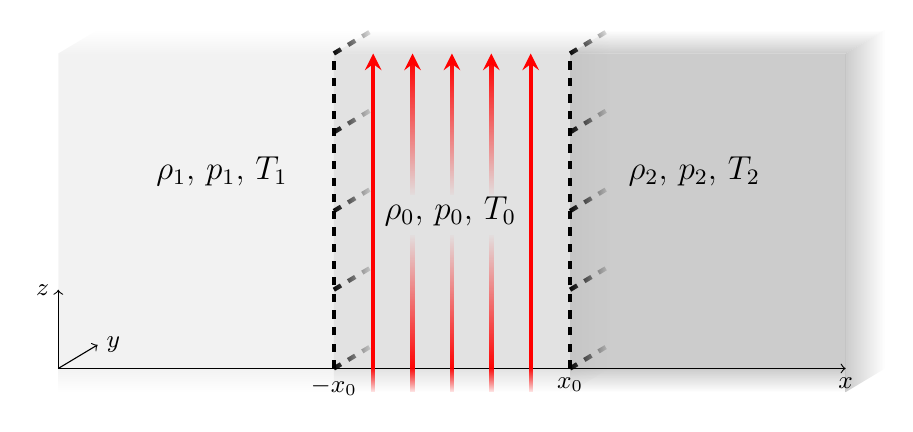
\begin{tikzpicture}
	\path [fill=lightgray, opacity=0.45] (3.5,0) -- (3.5,4) -- (6.5,4) -- (6.5,0) -- (3.5,0);
	\shade[left color=lightgray,right color=white, opacity=0.45] (6.5,0) -- (6.5,4) -- (7,4.3) -- (7,0.3) -- (6.5,0);
	\shade[top color=lightgray,bottom color=white, opacity=0.45] (3.5,0) -- (6.5,0) -- (6.5,-0.3) -- (3.5,-0.3) -- (3.5,0);
	\shade[top color=white,bottom color=lightgray, opacity=0.45] (3.5,4) -- (4,4.3) -- (7,4.3) -- (6.5,4) -- (3.5,4);
	\shade[left color=lightgray,right color=white, opacity=0.45] (6.5,0) -- (6.5,-0.3) -- (7,0) -- (7,0.3) -- (6.5,0);
	
	\path [fill=lightgray, opacity=0.8] (6.5,0) -- (6.5,4) -- (10,4) -- (10,0) -- (6.5,0);
	\shade[top color=lightgray,bottom color=white, opacity=0.8] (6.5,0) -- (10,0) -- (10,-0.3) -- (6.5,-0.3) -- (6.5,0);
	\shade[top color=white,bottom color=lightgray, opacity=0.8] (6.5,4) -- (7,4.3) -- (10.5,4.3) -- (10,4) -- (6.5,4);
	\shade[left color=lightgray,right color=white, opacity=0.8] (10,-0.3) -- (10,4) -- (10.5,4.3) -- (10.5,0) -- (10,-0.3);
	
	\path [fill=lightgray, opacity=0.2] (0,0) -- (0,4) -- (3.5,4) -- (3.5,0) -- (0,0);
	\shade[top color=lightgray,bottom color=white, opacity=0.2] (0,0) -- (3.5,0) -- (3.5,-0.3) -- (0,-0.3) -- (0,0);
	\shade[top color=white,bottom color=lightgray, opacity=0.2] (0,4) -- (0.5,4.3) -- (4,4.3) -- (3.5,4) -- (0,4);
	
	\draw [<->] (0,1) -- (0,0) -- (10,0);
	\draw [->] (0,0) -- (0.5,0.3);
	
	\draw [ultra thick, dashed] (3.5,0) -- (3.5,4);
	\draw [ultra thick, dashed, path fading=east] (3.5,0) -- (4,0.3);
	\draw [ultra thick, dashed, path fading=east] (3.5,4) -- (4,4.3);
	\draw [ultra thick, dashed, path fading=east] (3.5,2) -- (4,2.3);
	\draw [ultra thick, dashed, path fading=east] (3.5,1) -- (4,1.3);
	\draw [ultra thick, dashed, path fading=east] (3.5,3) -- (4,3.3);
	\draw [ultra thick, red, -stealth] (4,0) -- (4,4);
	\draw [ultra thick, red, path fading=south] (4,-0.3) -- (4,0);
	\draw [ultra thick, red, path fading=north] (4.5,0) -- (4.5, 1.7);
	\draw [ultra thick, red, path fading=south] (4.5,-0.3) -- (4.5,0);
	\draw [ultra thick, red, path fading=south] (4.5,2.2) -- (4.5,3.9);
	\draw [ultra thick, red, -stealth] (4.5,3.9) -- (4.5,4);
	\draw [ultra thick, red, path fading=north] (5,0) -- (5, 1.7);
	\draw [ultra thick, red, path fading=south] (5,-0.3) -- (5, 0);
	\draw [ultra thick, red, path fading=south] (5,2.2) -- (5,3.9);
	\draw [ultra thick, red, -stealth] (5,3.9) -- (5,4);
	\draw [ultra thick, red, path fading=north] (5.5,0) -- (5.5, 1.7);
	\draw [ultra thick, red, path fading=south] (5.5,-0.3) -- (5.5, 0);
	\draw [ultra thick, red, path fading=south] (5.5,2.2) -- (5.5,3.9);
	\draw [ultra thick, red, -stealth] (5.5,3.9) -- (5.5,4);
	\draw [ultra thick, red, -stealth] (6,0) -- (6,4);
	\draw [ultra thick, red, path fading=south] (6,-0.3) -- (6,0);
	\draw [ultra thick, dashed] (6.5,0) --(6.5,4);
	\draw [ultra thick, dashed, path fading=east] (6.5,0) -- (7,0.3);
	\draw [ultra thick, dashed, path fading=east] (6.5,4) -- (7,4.3);
	\draw [ultra thick, dashed, path fading=east] (6.5,2) -- (7,2.3);
	\draw [ultra thick, dashed, path fading=east] (6.5,1) -- (7,1.3);
	\draw [ultra thick, dashed, path fading=east] (6.5,3) -- (7,3.3);
	
	\small
	\node [below] at (3.5,0) {$-x_0$};
	\node [below] at (6.5,0) {$x_0$};
	\node [below] at (10,0) {$x$};
	\node [left] at (0,1) {$z$};
	\node [right] at (0.5,0.3) {$y$};
	
	\large
	\node [right] at (1.1,2.5) {$\rho_1$, $p_1$, $T_1$};
	\node [right] at (4,2) {$\rho_0$, $p_0$, $T_0$};
	\node [right] at (7.1,2.5) {$\rho_2$, $p_2$, $T_2$};
	\end{tikzpicture}
	\caption{The equilibrium state inside the slab, ($|x| \leq x_0$) and outside the slab, ($x < -x_0$ and $x > x_0$). The red arrows illustrate magnetic field lines, $B(x)\mathbf{\widehat{z}}$, and the dashed black lines indicate the boundaries of the slab. \textcolor{red}{Change to mag outside}}
	\label{fig: eq}
\end{figure}

To ensure that the model is in equilibrium, the total pressure in each external region must balance the total pressure in the internal region, namely
\begin{equation}
	p_1 + \frac{B_1^2}{2\mu_0} = p_0 + \frac{B_0^2}{2\mu_0} = p_2 + \frac{B_2^2}{2\mu_0}, \label{pressure balance}
\end{equation}
where $\mu_0$ is the permeability of free space. We can rewrite Equation~\eqref{pressure balance} as
\begin{equation}
\rho_i\left(c_i^2 + \frac{\gamma}{2}v_{Ai}^2\right) = \rho_j\left(c_j^2 + \frac{\gamma}{2}v_{Aj}^2\right), \quad \text{for} \quad i, j = 0, 1, 2, \label{sound speeds}
\end{equation}
where we define the sound and Alfv\'{e}n speeds in each region by $c_j = \sqrt{\gamma p_j/\rho_j}$ and $v_{Aj} = B_j/\sqrt{\mu\rho_j}$, respectively, for $j = 0, 1, 2$. The adiabatic index\footnote{The adiabatic index is assumed uniform across the whole domain under the single-fluid approximation.} is $\gamma$.


\subsection{The dispersion relation}

In the derivation of the dispersion relation, we decompose the linearised ideal MHD equations into Fourier forms then combine them into an ordinary differential equation (ODE) for the transverse velocity perturbation for each of the three plasma regions. After finding the general solution to each of these ODEs, we match the solutions across each interface at $\pm x_0$. The condition for the existence of non-trivial solutions will lead to the dispersion relation. In mathematical terms, we're converting a set of partial differential equations into ordinary differential equations into algebraic equations, into a single equation. From a form that we cannot solve into a form that we can.


\subsubsection{Derivation} \label{sec: asym slab DR der}

We begin with the ideal MHD equations, linearised around a static equilibrium with subscripts $j$, Equations~\eqref{cont eqn lin}-\eqref{ind eqn lin}. Taking the partial derivative with respect to time of Equation~\eqref{mom eqn lin} and eliminating $\bB$ using Equation~\eqref{ind eqn lin}, gives \textcolor{red}{Check whether the last - should be a + in the first two eqns below.}
\begin{align}
	\frac{\partial^2 v_x}{\partial t^2} &= \frac{\partial}{\partial x}\left[ (c_j^2 + v_{Aj}^2)\nabla\cdot\bv - v_{Aj}^2\frac{\partial v_z}{\partial z} \right] + v_{Aj}^2 \frac{\partial^2 v_x}{\partial z^2} \label{mom x} \\
	\frac{\partial^2 v_y}{\partial t^2} &= \frac{\partial}{\partial y}\left[ (c_j^2 + v_{Aj}^2)\nabla\cdot\bv - v_{Aj}^2\frac{\partial v_z}{\partial z} \right] + v_{Aj}^2 \frac{\partial^2 v_y}{\partial z^2} \label{mom y} \\
	\frac{\partial^2 v_z}{\partial t^2} &= c_j^2\frac{\partial}{\partial z}(\nabla\cdot\bv). \label{mom z}
\end{align}
Taking Fourier solutions like $f(\mathbf{x},t) = \hat{f}(x) \exp{i(ly + kz - \omega t)}$, where $\mathbf{k} = (0, l, k)$ is the wavenumber vector and $\omega$ is the angular frequency, for $\mathbf{v}$ in Equation~\eqref{mom y} gives
\begin{equation}
(k^2v_{Aj}^2 - \omega^2)\hat{v}_y = l((c_j^2 + v_{Aj}^2)(i\hat{v}_x' - l\hat{v}_y - k\hat{v}_z) + kv_{Aj}^2\hat{v}_z),
\end{equation}
where $' = d/dx$. If the component of the wavenumber in the $y$-direction is zero, \textit{i.e.} $l = 0$, then this equation reduces to
\begin{equation}
(k^2v_{Aj}^2 - \omega^2)\hat{v}_y(x) = 0,
\end{equation}
which yield two solutions. Firstly, $\omega^2 = k^2v_{Aj}^2$ is a solution corresponding to shear Alfv\'{e}n waves with different phase speed for each magnetic iso-surface (in this case surfaces parallel to the $yz$-plane). The second solution is $\hat{v}_y(x) = 0$ for all $x$ and therefore $v_y = 0$, \textit{i.e.} waves without perturbation component along the slab and perpendicular to the magnetic field. These solutions correspond to magneto-acoustic modes. Thus we have a decoupling of the shear Alfv\'{e}n modes from the magneto-acoustic modes.

Focusing from here on magneto-acoustic modes, we seek solutions of the Fourier form
\begin{equation}
\bv(\mathbf{x},t)=(\hat{v}_x(x)\textrm{e}^{i(kz-\omega{t})}, 0, \hat{v}_z(x)\textrm{e}^{i(kz-\omega{t})}),
\label{vcomponents}
\end{equation}
This restricts the investigation to magneto-acoustic waves propagating parallel to the equilibrium magnetic field, with velocity perturbation amplitude $\hat{v}_x(x)$ in the $x$-direction, and $\hat{v}_z(x)$ in the $z$-direction. With this ansatz, Equation~\eqref{mom y} degenerates and Equations~\eqref{mom x} and~\eqref{mom z} become
\begin{align}
&-\omega^2\hat{v}_x = (c_j^2+v_\textrm{Aj}^2)(\hat{v}_x'' + ik\hat{v}_z') - v_\textrm{Aj}^2ik\hat{v}_z'-v_\textrm{Aj}^2k^2\hat{v}_x, \label{mom x 2} \\
&-\omega^2\hat{v}_z = c_j^2ik(\hat{v}_x' + ik\hat{v}_z). \label{mom z 2}
\end{align}
These equations can be combined to give an ordinary differential equation for $\hat{v}_x$, namely
\begin{equation}
\hat{v}_x'' - m_j^2\hat{v}_x = 0, \quad \text{where} \quad
m_j^2 = \frac{(k^2v_\textrm{Aj}^2 - \omega^2)(k^2c_j^2 - \omega^2)}{(c_j^2 + v_\textrm{Aj}^2)(k^2c_\textrm{Tj}^2 - \omega^2)}. \label{v_x ODE}
\end{equation}
This is identical to the corresponding equation governing, for example, a tangential interface or a symmetric slab, derived in Sections~\ref{sec: MHD waves interface} and~\ref{sec: MHD waves sym slab} by \cite{rob81a,edw_etal82}.

Solutions of Equations~\eqref{v_x ODE} are a linear combination of hyperbolic functions. We restrict our model to waves trapped by the slab by imposing the boundary condition $\hat{v}_x \to 0$ as $|x| \to \infty$. Thus, the general solution for the velocity perturbation in the $x$-direction is
\begin{equation}
\hat{v}_x(x)=
\begin{cases}
A(\cosh{m_1x} + \sinh{m_1x}), & \text{if } x < -x_0, \\
B\cosh{m_0x} + C\sinh{m_0x}, & \text{if } |x| \leq {x_0}, \\
D(\cosh{m_2x} - \sinh{m_2x}), & \text{if  } x > x_0, 
\end{cases} \label{vsoln}
\end{equation}
where $A$, $B$, $C$, and $D$ are arbitrary constants (with respect to $x$). The remaining boundary conditions are continuity of velocity and total pressure across the slab boundaries at $x = \pm{x_0}$. With the aim of finding an expression for the total pressure perturbation, the Equations~\eqref{cont eqn lin} and~\eqref{energy eqn lin} can be combined to give
\begin{equation}
	\frac{\partial p}{\partial t} = - \rho_jc_i^2\nabla\cdot\bv.
\end{equation}
Using the above equation and the $z$-component of Equation~\eqref{ind eqn lin}, the perturbation in total pressure (plasma pressure, $p$, plus magnetic pressure, $B_jB_z/\mu$) across the whole domain can be shown to have amplitude
\begin{equation}
\hat{p}_T(x) = \frac{\Lambda_j}{m_j}\hat{v}_x'(x),
\end{equation}
where
\begin{equation}
\Lambda_j = \frac{i\rho_j(\omega^2 - \omega_{Aj}^2)}{m_j\omega}, \quad \text{for} \quad j = 0, 1, 2. \label{Lambdas}
\end{equation}
Ensuring continuity of velocity and total pressure across the slab boundaries gives four coupled algebraic equations, namely
\begin{equation}
\left(
\begin{matrix}
c_1-s_1             &-c_0           &s_0            &0                   \\
0                   &c_0            &s_0            &s_2-c_2             \\
\Lambda_1(c_1-s_1)  &\Lambda_0s_0   &-\Lambda_0c_0  &0                   \\
0                   &\Lambda_0s_0   &\Lambda_0c_0   &-\Lambda_2(s_2-c_2)
\end{matrix}
\right)
\left(
\begin{matrix}
A \\
B \\
C \\
D
\end{matrix}
\right)
=
\left(
\begin{matrix}
0 \\
0 \\
0 \\
0
\end{matrix}
\right),
\label{coefmatrix}
\end{equation}
where $c_j = \cosh{m_jx_0}$ and $s_j = \sinh{m_jx_0}$ for $j=0,1,2$, for brevity. The condition for the existence of non-trivial solutions to this system of equations is that the determinant of the matrix is zero. Applying this condition gives us the dispersion relation for an asymmetric slab, namely
\begin{equation}
(\Lambda_0^2 + \Lambda_1\Lambda_2) + \Lambda_0(\Lambda_1 + \Lambda_2)\coth{2m_0x_0} = 0. \label{DR lambda}
\end{equation}
By expanding each $\Lambda_j$, we can write this dispersion relation in familiar variables as
\begin{align}
&m_0^2(\omega^2 - \omega_{A1}^2)(\omega^2 - \omega_{A2}^2) + \frac{\rho_0}{\rho_1}m_1\frac{\rho_0}{\rho_2}m_2(\omega^2 - \omega_{A0}^2)^2 \notag \\
& + m_0(\omega^2 - \omega_{A0}^2)\left[\frac{\rho_0}{\rho_1}m_1(\omega^2 - \omega_{A2}^2) + \frac{\rho_0}{\rho_2}m_2(\omega^2 - \omega_{A1}^2)\right]\coth{2m_0x_0} = 0. \label{DR}
\end{align}


\subsubsection{First-order asymmetric slab}

There is a qualitative difference between waves propagating along symmetric and asymmetric magnetic slabs. The dispersion relation governing an asymmetric slab is a single equation, whereas the dispersion relation governing a symmetric slab \citep{rob81a} consists of two independent equations, corresponding to the sausage and kink eigenmodes.

Under the approximation that the densities and temperatures of the external plasma are of the same order, the dispersion relation, Equation~\eqref{DR}, can be factorised to give the approximate dispersion relation
\begin{equation}
\left[\Lambda_0(\Lambda_1+\Lambda_2)+2\Lambda_1\Lambda_2\tanh{m_0x_0}\right]\left[\Lambda_0(\Lambda_1+\Lambda_2)+2\Lambda_1\Lambda_2\coth{m_0x_0}\right]=0. \label{DR approx lambda}
\end{equation}
To show this, define each bracket as the following functions
\begin{align}
D_s(\omega) &:= \Lambda_0(\Lambda_1 + \Lambda_2) + 2\Lambda_1\Lambda_2\tanh{m_0x_0}, \\
D_k(\omega) &:= \Lambda_0 (\Lambda_1 + \Lambda_2) + 2\Lambda_1\Lambda_2\coth{m_0x_0}.
\end{align}
There product is
\begin{align}
D_s(\omega)D_k(\omega) &= \left[ \Lambda_0(\Lambda_1 + \Lambda_2) + 2\Lambda_1\Lambda_2\tanh{m_0x_0} \right] \left[ \Lambda_0 (\Lambda_1 + \Lambda_2) + 2\Lambda_1\Lambda_2\coth{m_0x_0} \right] \\
&= \Lambda_0^2 (\Lambda_1 + \Lambda_2)^2 + 2\Lambda_0(\Lambda_1 + \Lambda_2)\Lambda_1\Lambda_2(\tanh{m_0x_0} + \coth{m_0x_0}) + 4\Lambda_1^2\Lambda_2^2 \\
&= 4\Lambda_1\Lambda_2 \left[ (\Lambda_0^2F + \Lambda_1\Lambda_2) + \Lambda_0(\Lambda_1 + \Lambda_2)\coth(2m_0x_0) \right] \\
\end{align}
where
\begin{equation}
F = \frac{(\Lambda_1 + \Lambda_2)^2}{4\Lambda_1\Lambda_2}.
\end{equation}
When the plasma parameters on each side of the slab are approximately equal, \textit{i.e.} $\Lambda_2 = \Lambda_1 (1 + \epsilon L)$, with $\epsilon \ll 1$ and $L \approx 1$, $F$ becomes
\begin{equation}
F = \frac{(2 + \epsilon L)^2}{4(1 + \epsilon L)} = 1 + \mathcal{O}(\epsilon^2).
\end{equation}
Therefore, 
\begin{equation}
(\Lambda_0^2 + \Lambda_1\Lambda_2) + \Lambda_0(\Lambda_1 + \Lambda_2)\coth(2m_0x_0) = \frac{1}{4\Lambda_1\Lambda_2} D_s(\omega) D_k(\omega) + \mathcal{O}(\epsilon^2).
\end{equation}
Therefore, to linear order of waveguide asymmetry, if the dispersion relation, Equation~\eqref{DR lambda} is satisfied, then either $D_s(\omega) = 0$ or $D_k(\omega) = 0$, which completes the proof of Equation~\eqref{DR approx lambda}.

The expressions for the variables $\Lambda_i$ for $i=0,1,2$ in Equations~\eqref{Lambdas} can be employed to yield the approximately symmetric dispersion relation
\begin{equation}
(\omega^2 - \omega_{A0}^2)\left(\frac{\rho_0}{\rho_1}\frac{m_1}{(\omega^2 - \omega_{A1}^2)} + \frac{\rho_0}{\rho_2}\frac{m_2}{(\omega^2 - \omega_{A2}^2)}\right) + 2m_0\left(\begin{matrix}\tanh \\ \coth \end{matrix}\right)(m_0x_0) = 0. \label{DR approx}
\end{equation}
This equation is now in a form similar to Equation~\eqref{DR sym slab}, the dispersion relation corresponding to MHD waves along a symmetric magnetic slab (Section~\ref{sec: MHD waves sym slab}), namely
\begin{equation}
\rho_im_e(\omega^2 - \omega_\textrm{Ai}^2) + \rho_em_i(\omega^2 - \omega_\textrm{Ae}^2)\left(\begin{matrix}\tanh \\ \coth \end{matrix}\right)(m_ix_0) = 0, \label{DRsym}
\end{equation}
where internal and external parameters are denoted by subscripts $i$ and $e$.


\subsection{Asymmetric eigenmodes}
There is a rich spectrum of MHD eigenmodes on an asymmetric magnetic slab. The key distinctions of these modes from the eigenmodes of a symmetric slab are discussed in this subsection. To aid the reader's understanding, we have created over a hundred 3D animations of symmetric and asymmetric eigenmodes in a magnetic slab \cite{all_etal18c}. The videos visualise the oscillations in the slab boundaries, magnetic field, density, and velocity field. \textcolor{red}{Consider including figure screenshots of the videos and describing/explaining them.}

The dispersion relation for a symmetric slab, Equation~\eqref{DRsym}, consists of two decoupled equations that correspond to the two types of eigenmodes supported by the slab: the \textit{sausage} and \textit{kink} MHD waves. In an asymmetric slab, the sausage and kink modes are modified by the external density difference, causing an asymmetry of the oscillation amplitude on each side of the slab (for visualisation see Figures~\ref{fig:saus} and~\ref{fig:kink}). We call these asymmetric eigenmodes quasi-sausage and quasi-kink modes. In a symmetric slab, sausage modes are characterised by an undisplaced slab axis in the centre of the slab. In an asymmetric slab, this undisplaced position is shifted towards the side of greatest external density for kink modes and towards the side of lowest external density for sausage modes. For symmetric kink modes, the width of the perturbed slab remains constant along the slab, but this characteristic is lost in an asymmetric slab. This highlights the mixed nature of these modes. 

Additionally, this shows that it is the phase of the boundary oscillations that is a more fundamental distinguishing characteristic of sausage and kink modes. For this reason, when we refer to \textit{sausage} and \textit{kink} modes of an asymmetric slab, we refer strictly to modes with boundary oscillations in \textit{anti-phase} and \textit{in-phase}, respectively. The differences between symmetric and asymmetric eigenmodes are summarised in Table~\ref{tab: eigenmode differences}.

\begin{figure}
	\makebox[\textwidth][c]{
		\subfloat[Quasi-kink]{\scalebox{1}{
				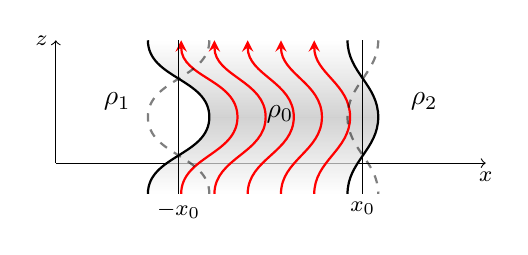
\begin{tikzpicture}[scale=0.78]
				\draw [->] (0,0) -- (7,0);
				
				\shade[bottom color=lightgray,top color=white, opacity=0.7] (1.5,2) to [out=-90,in=90] (2.5,0.75) to (5.25,0.75) to [out=90,in=-90] (4.75,2) to (1.5,2);
				
				\shade[bottom color=white,top color=lightgray, opacity=0.7] (2.5,0.75) to (5.25,0.75) to [out=-90,in=90] (4.75,-0.5) to (1.5,-0.5) to [out=90,in=-90] (2.5,0.75);
				
				\draw [thick] (1.5,2) to [out=-90,in=90] (2.5,0.75) to [out=-90,in=90] (1.5,-0.5);
				\draw [thick] (4.75,2) to [out=-90,in=90] (5.25,0.75) to [out=-90,in=90] (4.75,-0.5);
				
				\draw [thick, red, -stealth] (2.0417,-0.5) to [out=90,in=-90] (2.9583, 0.75) to [out=90,in=-90] (2.0417,2);
				\draw [thick, red, -stealth] (2.5833,-0.5) to [out=90,in=-90] (3.4167, 0.75) to [out=90,in=-90] (2.5833,2);
				\draw [thick, red, -stealth] (3.125,-0.5) to [out=90,in=-90] (3.875, 0.75) to [out=90,in=-90] (3.125,2);
				\draw [thick, red, -stealth] (3.6667,-0.5) to [out=90,in=-90] (4.3333, 0.75) to [out=90,in=-90] (3.6667,2);
				\draw [thick, red, -stealth] (4.2083,-0.5) to [out=90,in=-90] (4.7917, 0.75) to [out=90,in=-90] (4.2083,2);
				
				\draw [thick, dashed, opacity=0.5] (2.5,2) to [out=-90,in=90] (1.5,0.75) to [out=-90,in=90] (2.5,-0.5);
				\draw [thick, dashed, opacity=0.5] (5.25,2) to [out=-90,in=90] (4.75,0.75) to [out=-90,in=90] (5.25,-0.5);
				
				% % % % % % % % % % % % % % % % % % % % % % % % % %
				
				\draw [->] (0,0) -- (0,2);
				
				\node at (1,1) {$\rho_1$};
				\node at (6,1) {$\rho_2$};
				\node at (3.65,0.8) {$\rho_0$};
				
				\footnotesize
				\node [below] at (2,-0.5) {$-x_0$};
				\node [below] at (5,-0.5) {$x_0$};
				
				\node [left] at (0,2) {$z$};
				\node [below] at (7,0) {$x$};
				\draw [-] (2,-0.5) -- (2,2);
				\draw [-] (5,-0.5) -- (5,2);
				\end{tikzpicture}
				\label{fig:saus}}}
		%
		%
		%
		%
		\subfloat[Quasi-sausage]{\scalebox{1}{
				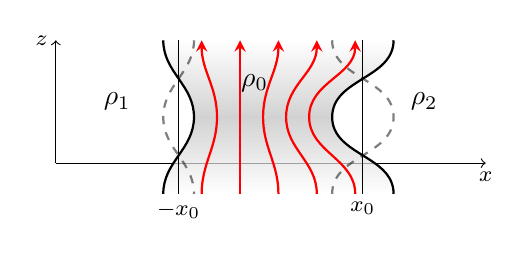
\begin{tikzpicture}[scale=0.78]
				\draw [->] (0,0) -- (7,0);
				
				\shade[bottom color=lightgray,top color=white, opacity=0.7] (1.75,2) to [out=-90,in=90] (2.25,0.75) to (4.5,0.75) to [out=90,in=-90] (5.5,2) to (1.75,2);
				
				\shade[bottom color=white,top color=lightgray, opacity=0.7] (2.25,0.75) to (4.5,0.75) to [out=-90,in=90] (5.5,-0.5) to (1.75,-0.5) to [out=90,in=-90] (2.25,0.75);
				
				\draw [thick] (1.75,2) to [out=-90,in=90] (2.25,0.75) to [out=-90,in=90] (1.75,-0.5);
				\draw [thick, dashed, opacity=0.5] (4.5,2) to [out=-90,in=90] (5.5,0.75) to [out=-90,in=90] (4.5,-0.5);
				
				\draw [thick, red, -stealth] (2.375,-0.5) to [out=90,in=-90] (2.625, 0.75) to [out=90,in=-90] (2.375,2);
				\draw [thick, red, -stealth] (3,-0.5) to [out=90,in=-90] (3, 0.75) to [out=90,in=-90] (3,2);
				\draw [thick, red, -stealth] (3.625,-0.5) to [out=90,in=-90] (3.375, 0.75) to [out=90,in=-90] (3.625,2);
				\draw [thick, red, -stealth] (4.25,-0.5) to [out=90,in=-90] (3.75, 0.75) to [out=90,in=-90] (4.25,2);
				\draw [thick, red, -stealth] (4.875,-0.5) to [out=90,in=-90] (4.125, 0.75) to [out=90,in=-90] (4.875,2);
				
				\draw [thick, dashed, opacity=0.5] (2.25,2) to [out=-90,in=90] (1.75,0.75) to [out=-90,in=90] (2.25,-0.5);
				\draw [thick] (5.5,2) to [out=-90,in=90] (4.5,0.75) to [out=-90,in=90] (5.5,-0.5);
				
				% % % % % % % % % % % % % % % % % % % % % % % % % %
				
				\draw [->] (0,0) -- (0,2);
				
				\node at (1,1) {$\rho_1$};
				\node at (6,1) {$\rho_2$};
				\node [right] at (2.86,1.3) {$\rho_0$};
				
				\footnotesize
				\node [below] at (2,-0.5) {$-x_0$};
				\node [below] at (5,-0.5) {$x_0$};
				
				\node [left] at (0,2) {$z$};
				\node [below] at (7,0) {$x$};
				\draw [-] (2,-0.5) -- (2,2);
				\draw [-] (5,-0.5) -- (5,2);
				\end{tikzpicture}
				\label{fig:kink}}}}
	\caption{Quasi-kink and quasi-sausage modes with external density ordering $\rho_1>\rho_2$. The red lines illustrate the perturbed magnetic field, the thick solid black lines illustrate the perturbed slab boundaries, and the dashed lines illustrate the future position of the slab boundaries after half a period. \textcolor{red}{remove arrows}}
\end{figure}

Sausage and kink modes are further categorised into \textit{surface} and \textit{body} modes. Surface modes are waves more enhanced at the slab boundaries, whereas body waves are characterised by oscillations permeating spatially throughout the slab, having their maximum amplitude within the slab. Mathematically, surface waves correspond to exponentially damped solutions of Equation~\eqref{vsoln} within the slab. This occurs when $m_0^2 > 0$, which occurs when the phase speed, $\omega/k$, satisfies
\begin{equation}
\frac{\omega}{k}<c_\textrm{T} \quad \text{or} \quad \text{min}\{c_0, v_\textrm{A}\}<\frac{\omega}{k}<\text{max}\{c_0, v_\textrm{A}\}.
\end{equation}
Body waves correspond to trigonometric solutions of Equation~\eqref{vsoln} within the slab. Most notably, this means that there are any number of nodes within the slab where the plasma is unperturbed, so that there exist an infinite set of body eigenmodes. They exist when $m_0^2 < 0$, which occurs when
\begin{equation}
c_\textrm{T}<\frac{\omega}{k}<\text{min}\{c_0, v_\textrm{A}\} \quad \text{or} \quad \text{max}\{c_0, v_\textrm{A}\}<\frac{\omega}{k}. \label{bconditions}
\end{equation}

For a surface mode (Figures~\ref{fig:surf quasi-kink} and~\ref{fig:surf quasi-saus}), the wave power distribution across the slab has a single minimum. The displacement of this minimum from the centre of the slab is a consequence of the asymmetry in the external plasma. The intensity of the maximum amplitudes on the left and right boundaries of the slab is different, reflecting the asymmetry in the external plasma.

Body modes are also affected by the asymmetric external environment (Figures~\ref{fig:body quasi-kink} and~\ref{fig:body quasi-saus}). Local maxima and minima in wave power are shifted towards the external plasma of higher density for a quasi-kink body mode and towards the external plasma of lower density for a quasi-sausage mode. However, this is a much weaker effect than for surface modes because the eigenfrequencies of body waves do not depend strongly on the parameters of the external plasma, and therefore they do not depend strongly on the asymmetry of the waveguide, as shown in Sections~\ref{sec: analytical solutions} and~\ref{sec: numerical solutions}. The same can be said for the eigenfunctions of body modes. These results corroborate the intuition that because the majority of the wave power is confined to within the slab, rather than its boundaries, the body modes don't \textit{feel} the external plasma as much as surface waves do.

\begin{table}
	\centering
	\begin{tabular}{ccccc}
		\toprule
		\multirow{2}{*}{Mode type} & Boundary & Constant & Axis & Unperturbed \\
		 & oscillations & width & displacement & position \\
		\midrule
		Symmetric sausage & Anti-phase & No & No & Middle \\
		Asymmetric sausage & Anti-phase & No & Yes & Shifted \\
		Symmetric kink & In-phase & Yes & Yes & - \\
		Asymmetric kink & In-phase & No	& Yes & - \\
		\bottomrule
	\end{tabular}
	\caption{The qualitative differences between symmetric and asymmetric surface modes.}
	\label{tab: eigenmode differences}
\end{table}

\begin{figure}
	\makebox[\textwidth][c]{
		\subfloat[Quasi-kink surface mode]{\scalebox{1}{
				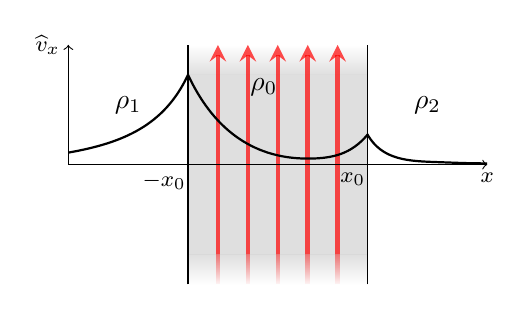
\begin{tikzpicture}[scale=0.76]
				\path [fill=lightgray, opacity=0.5] (2,-1.5) -- (2,1.5) -- (5,1.5) -- (5,-1.5) -- (2,-1.5);
				
				\shade[bottom color=white,top color=lightgray, opacity=0.5] (2,-2) to (5,-2) to (5,-1.5) to (2,-1.5) to (2,-2);
				
				\shade[top color=white,bottom color=lightgray, opacity=0.5] (2,2) to (5,2) to (5,1.5) to (2,1.5) to (2,2);
				
				\draw [-] (2,-2) -- (2,2);
				\draw [-] (5,-2) -- (5,2);
				
				\draw [ultra thick, red, -stealth,opacity=0.7] (2.5,-1.5) -- (2.5,2);
				\draw [ultra thick, red, path fading=south, opacity=0.5] (2.5,-2) -- (2.5,-1.5);
				\draw [ultra thick, red, -stealth,opacity=0.7] (3,-1.5) -- (3,2);
				\draw [ultra thick, red, path fading=south,opacity=0.5] (3,-2) -- (3,-1.5);
				\draw [ultra thick, red, -stealth,opacity=0.7] (3.5,-1.5) -- (3.5,2);
				\draw [ultra thick, red, path fading=south,opacity=0.5] (3.5,-2) -- (3.5,-1.5);
				\draw [ultra thick, red, -stealth,opacity=0.7] (4,-1.5) -- (4,2);
				\draw [ultra thick, red, path fading=south,opacity=0.5] (4,-2) -- (4,-1.5);
				\draw [ultra thick, red, -stealth,opacity=0.7] (4.5,-1.5) -- (4.5,2);
				\draw [ultra thick, red, path fading=south,opacity=0.5] (4.5,-2) -- (4.5,-1.5);
				
				\draw [thick] (0,0.2) to [out=10, in=245] (2, 1.5) to [out=295, in=180] (4,0.1) to [out=0, in=230] (5,0.5) to [out=300, in=178] (6.2,0.04) to [out=358, in=180] (7,0.02);
				
				\draw [->] (0,0) -- (0,2);
				\draw [->] (0,0) -- (7,0);
				
				\node at (1,1) {$\rho_1$};
				\node at (6,1) {$\rho_2$};
				\node [right] at (2.88,1.3) {$\rho_0$};
				
				\footnotesize
				\node [below left] at (2.1,0) {$-x_0$};
				\node [below left] at (5.1,0) {$x_0$};
				
				\node [left] at (0,2) {$\widehat{v}_x$};
				\node [below] at (7,0) {$x$};
				\end{tikzpicture}
				\label{fig:surf quasi-kink}}}
		%
		%
		%
		%
		\subfloat[Quasi-sausage surface mode]{\scalebox{1}{
				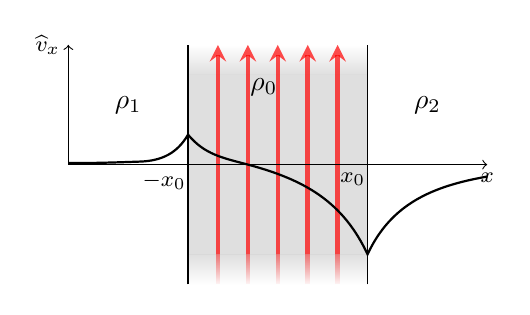
\begin{tikzpicture}[scale=0.76]
				\path [fill=lightgray, opacity=0.5] (2,-1.5) -- (2,1.5) -- (5,1.5) -- (5,-1.5) -- (2,-1.5);
				
				\shade[bottom color=white,top color=lightgray, opacity=0.5] (2,-2) to (5,-2) to (5,-1.5) to (2,-1.5) to (2,-2);
				
				\shade[top color=white,bottom color=lightgray, opacity=0.5] (2,2) to (5,2) to (5,1.5) to (2,1.5) to (2,2);
				
				\draw [-] (2,-2) -- (2,2);
				\draw [-] (5,-2) -- (5,2);
				
				\draw [ultra thick, red, -stealth,opacity=0.7] (2.5,-1.5) -- (2.5,2);
				\draw [ultra thick, red, path fading=south, opacity=0.5] (2.5,-2) -- (2.5,-1.5);
				\draw [ultra thick, red, -stealth,opacity=0.7] (3,-1.5) -- (3,2);
				\draw [ultra thick, red, path fading=south,opacity=0.5] (3,-2) -- (3,-1.5);
				\draw [ultra thick, red, -stealth,opacity=0.7] (3.5,-1.5) -- (3.5,2);
				\draw [ultra thick, red, path fading=south,opacity=0.5] (3.5,-2) -- (3.5,-1.5);
				\draw [ultra thick, red, -stealth,opacity=0.7] (4,-1.5) -- (4,2);
				\draw [ultra thick, red, path fading=south,opacity=0.5] (4,-2) -- (4,-1.5);
				\draw [ultra thick, red, -stealth,opacity=0.7] (4.5,-1.5) -- (4.5,2);
				\draw [ultra thick, red, path fading=south,opacity=0.5] (4.5,-2) -- (4.5,-1.5);
				
				\draw [thick] (0,0.025) to [out=0, in=-178] (1.2, 0.05) to [out=2, in=-120] (2,0.5) to [out=-50, in=165] (3,0) to [out=-15, in=115] (5,-1.5) to [out=65, in=-170] (7,-0.2);
				\draw [->] (0,0) -- (0,2);
				\draw [->] (0,0) -- (7,0);
				
				\node at (1,1) {$\rho_1$};
				\node at (6,1) {$\rho_2$};
				\node [right] at (2.88,1.3) {$\rho_0$};
				
				\footnotesize
				\node [below left] at (2.1,0) {$-x_0$};
				\node [below left] at (5.1,0) {$x_0$};
				
				\node [left] at (0,2) {$\widehat{v}_x$};
				\node [below] at (7,0) {$x$};
				\end{tikzpicture}
				\label{fig:surf quasi-saus}}}}
	%
	%
	\\
	%
	%
	\makebox[\textwidth][c]{
		\subfloat[Quasi-kink body mode]{\scalebox{1}{
				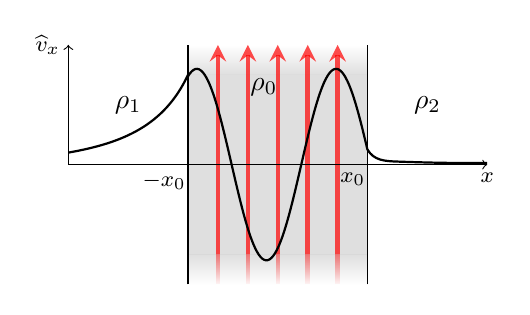
\begin{tikzpicture}[scale=0.76]
				\path [fill=lightgray, opacity=0.5] (2,-1.5) -- (2,1.5) -- (5,1.5) -- (5,-1.5) -- (2,-1.5);
				
				\shade[bottom color=white,top color=lightgray, opacity=0.5] (2,-2) to (5,-2) to (5,-1.5) to (2,-1.5) to (2,-2);
				
				\shade[top color=white,bottom color=lightgray, opacity=0.5] (2,2) to (5,2) to (5,1.5) to (2,1.5) to (2,2);
				
				\draw [-] (2,-2) -- (2,2);
				\draw [-] (5,-2) -- (5,2);
				
				\draw [thick] (7,0.025) to [out=180, in=358] (5.5, 0.05) to [out=178, in=300] (5,0.25);
				
				
				\draw [ultra thick, red, -stealth,opacity=0.7] (2.5,-1.5) -- (2.5,2);
				\draw [ultra thick, red, path fading=south, opacity=0.5] (2.5,-2) -- (2.5,-1.5);
				\draw [ultra thick, red, -stealth,opacity=0.7] (3,-1.5) -- (3,2);
				\draw [ultra thick, red, path fading=south,opacity=0.5] (3,-2) -- (3,-1.5);
				\draw [ultra thick, red, -stealth,opacity=0.7] (3.5,-1.5) -- (3.5,2);
				\draw [ultra thick, red, path fading=south,opacity=0.5] (3.5,-2) -- (3.5,-1.5);
				\draw [ultra thick, red, -stealth,opacity=0.7] (4,-1.5) -- (4,2);
				\draw [ultra thick, red, path fading=south,opacity=0.5] (4,-2) -- (4,-1.5);
				\draw [ultra thick, red, -stealth,opacity=0.7] (4.5,-1.5) -- (4.5,2);
				\draw [ultra thick, red, path fading=south,opacity=0.5] (4.5,-2) -- (4.5,-1.5);
				
				\draw [thick, smooth, samples=100, domain=2:5] plot (\x,{1.6*cos(2.7*(\x+0.18) r)});
				
				\draw [thick] (0,0.2) to [out=10, in=245] (2, 1.5);
				
				\draw [->] (0,0) -- (0,2);
				\draw [->] (0,0) -- (7,0);
				
				\node at (1,1) {$\rho_1$};
				\node at (6,1) {$\rho_2$};
				\node [right] at (2.88,1.3) {$\rho_0$};
				
				\footnotesize
				\node [below left] at (2.1,0) {$-x_0$};
				\node [below left] at (5.1,0) {$x_0$};
				
				\node [left] at (0,2) {$\widehat{v}_x$};
				\node [below] at (7,0) {$x$};
				\end{tikzpicture}
				\label{fig:body quasi-kink}}}
		%
		%
		%
		%
		\subfloat[Quasi-sausage body mode]{\scalebox{1}{
				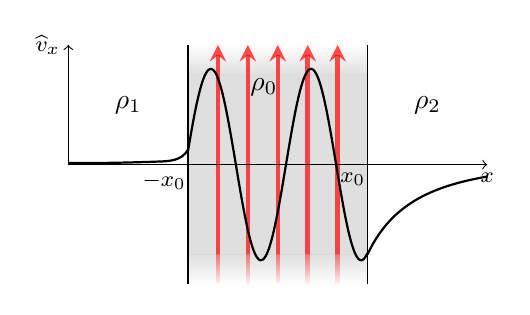
\begin{tikzpicture}[scale=0.76]
				\path [fill=lightgray, opacity=0.5] (2,-1.5) -- (2,1.5) -- (5,1.5) -- (5,-1.5) -- (2,-1.5);
				
				\shade[bottom color=white,top color=lightgray, opacity=0.5] (2,-2) to (5,-2) to (5,-1.5) to (2,-1.5) to (2,-2);
				
				\shade[top color=white,bottom color=lightgray, opacity=0.5] (2,2) to (5,2) to (5,1.5) to (2,1.5) to (2,2);
				
				\draw [-] (2,-2) -- (2,2);
				\draw [-] (5,-2) -- (5,2);
				
				\draw [thick] (0,0.025) to [out=0, in=-178] (1.5, 0.05) to [out=2, in=-120] (2,0.25);
				
				\draw [ultra thick, red, -stealth,opacity=0.7] (2.5,-1.5) -- (2.5,2);
				\draw [ultra thick, red, path fading=south, opacity=0.5] (2.5,-2) -- (2.5,-1.5);
				\draw [ultra thick, red, -stealth,opacity=0.7] (3,-1.5) -- (3,2);
				\draw [ultra thick, red, path fading=south,opacity=0.5] (3,-2) -- (3,-1.5);
				\draw [ultra thick, red, -stealth,opacity=0.7] (3.5,-1.5) -- (3.5,2);
				\draw [ultra thick, red, path fading=south,opacity=0.5] (3.5,-2) -- (3.5,-1.5);
				\draw [ultra thick, red, -stealth,opacity=0.7] (4,-1.5) -- (4,2);
				\draw [ultra thick, red, path fading=south,opacity=0.5] (4,-2) -- (4,-1.5);
				\draw [ultra thick, red, -stealth,opacity=0.7] (4.5,-1.5) -- (4.5,2);
				\draw [ultra thick, red, path fading=south,opacity=0.5] (4.5,-2) -- (4.5,-1.5);
				
				%\draw [thick] (2,0.5) to [out=-50, in=180] (2.3,0.25) to [out=0, in=180] (3.2,1) to [out=0, in=180] (4.1,0.1) to [out=-0, in=-120] (5,1.5);
				
				\draw [thick, smooth, samples=100, domain=2:5] plot (\x,{1.6*cos(3.75*(\x-0.705) r)});
				
				\draw [thick] (5,-1.5) to [out=65, in=-170] (7,-0.2);
				
				\draw [->] (0,0) -- (0,2);
				\draw [->] (0,0) -- (7,0);
				
				\node at (1,1) {$\rho_1$};
				\node at (6,1) {$\rho_2$};
				\node [right] at (2.88,1.3) {$\rho_0$};
				
				\footnotesize
				\node [below left] at (2.1,0) {$-x_0$};
				\node [below left] at (5.1,0) {$x_0$};
				
				\node [left] at (0,2) {$\widehat{v}_x$};
				\node [below] at (7,0) {$x$};
				\end{tikzpicture}
				\label{fig:body quasi-saus}}}}
	\caption{The transverse velocity perturbation amplitude, $\widehat{v}_x$ as a function of the transverse spatial coordinate, $x$, for quasi-sausage and quasi-kink modes in an isolated magnetic slab with external density ordering $\rho_1 > \rho_2$. \textcolor{red}{remove shading and arrows}}
\end{figure}


%------------------------------------------------------------------------------
\section{Asymmetric slab in a non-magnetic environment}
\label{sec: EVP non-mag}
%------------------------------------------------------------------------------

Much of the interesting physics due to waveguide asymmetry is exhibited by a magnetic slab with non-magnetic external plasma. We study this system in this Section.

By letting $B_1 = B_2 = 0$, the plasma in the asymmetric external regions is non-magnetic. Then the dispersion relation, Equation~\eqref{DR}, simplifies to
\begin{equation}
m_0^2\omega^4 + \frac{\rho_0}{\rho_1}m_1\frac{\rho_0}{\rho_2}m_2(\omega^2 - \omega_\textrm{A0}^2)^2 + m_0\omega^2(\omega^2 - \omega_{A0}^2)\left(\frac{\rho_0}{\rho_1}m_1 + \frac{\rho_0}{\rho_2}m_2\right)\coth{2m_0x_0} = 0, \label{DR non-mag}
\end{equation}
and the dispersion relation for a slab with first order asymmetry simplifies to
\begin{equation}
(\omega^2 - \omega_\textrm{A0}^2)\left(\frac{\rho_0}{\rho_1}m_1 + \frac{\rho_0}{\rho_2}m_2\right)  +  2\omega^2m_0\left(\begin{matrix}\tanh \\ \coth \end{matrix}\right)(m_0x_0) = 0. \label{DR approx non-mag}
\end{equation}


\subsection{Analytical solutions}
Analytical solutions to the dispersion relation can only be made under further assumptions about the plasma. In this section, incompressible (Section~\ref{sec: incomp}), zero-beta (Section~\ref{sec: zero-beta}), thin slab (Section~\ref{sec: thin slab}), and wide slab (Section~\ref{sec: wide slab}) approximations are explored. First, we deal with spurious solutions in Section~\ref{sec: spurious}.

\subsubsection{Spurious solutions} \label{sec: spurious}
There are three sets of spurious roots to the dispersion relation, $\omega = \pm kv_{A0}$, $\omega = \pm kc_0$, and $\omega = \pm kc_{T0}$. To treat these cases we refer back to the ODE for $\hat{v}_x(x)$ within the slab, Equation~\eqref{v_x ODE}.

When $\omega = \pm kc_{T0}$, $m_0$ is singular, in which case the solution to Equation~\eqref{v_x ODE} is $\hat{v}_x(x) = 0$ within the slab. From Equation\eqref{mom z 2}, it follows that $\hat{v}_z \propto \hat{v}_x'$, we therefore also have $\hat{v}_z(x) = 0$. Given that we are assuming ideal plasma so that the magnetic flux is frozen to the plasma, this means that there is no magnetic field perturbation either. Therefore, $\omega = \pm kc_{T0}$ is a spurious solution.

\textcolor{red}{edit from below here on spurious sols.}

When $\omega = \pm kc_0$, we have $m_0 = 0$, therefore Equation~\eqref{v_x ODE} has general solution $\hat{v}_x(x) = Bx + C$ for constants $B$ and $C$. Equation~\eqref{mom z 2} further shows that  $\hat{v}_x' = 0$. Therefore, $B = 0$ and $\hat{v}_x(x) = C$. The $z$-component of Equation~\eqref{ind eqn lin} tells us that $\hat{b}_z \propto \hat{v}_x'$ and so $\hat{b}_z = 0$, therefore the magnetic pressure perturbation is zero. It can be shown that the plasma pressure is
\begin{equation}
\hat{p}(x) = - \frac{i\rho_0c_0^2}{\omega}\left[\frac{Cx(k^2v_A^2 - \omega^2)}{c_0^2} + C_2\right],
\end{equation}
within the slab, for constant $C_2$. To make pressure balance over each interface we must have $C=0$. This means that $v_x(x)=0$ within the slab and therefore across the whole domain. Therefore the pressure outside the slab is zero (since it is proportional to $\hat{v}_x' = 0$) , and by matching pressure, it is zero within the slab. Therefore this solution is a trivial wave. (is this the entropy wave???)

On the other hand, when $\omega = kv_A$, the total pressure amplitude, $\hat{P}(x)$, is such that
\begin{equation}
\widehat{P}(x)=\widehat{v}_x'(x)
\begin{cases}
\Lambda_1/m_1, & \text{if } x<-x_0, \\
\Lambda_0/m_0, & \text{if }|x|\leq{}x_0, \\
\Lambda_2/m_2, & \text{if }x>x_0,
\end{cases}
\end{equation}
where
\begin{equation}
\Lambda_0=-\frac{i\rho_0(k^2v_\textrm{A}^2-\omega^2)}{m_0\omega}, \quad \Lambda_1=\frac{i\rho_1\omega}{m_1}, \quad \text{and} \quad \Lambda_2=\frac{i\rho_2\omega}{m_2}. \label{Lambdas}
\end{equation}
(the derivation for this still holds). Note that the singularity due to the division by $m_0^2$ is regulated by the factor of $k^2v_A^2 - \omega^2$ in $\Lambda_0$. Therefore, since $\hat{v}_x' = B$ is constant in the slab, then so is $\hat{P}$. When we match the total pressure over the boundaries we find that the slab must be symmetric. Therefore $B=0$ to ensure that the velocity profile is symmetric. Therefore $\hat{v}_x' = B = 0$, so there is no pressure perturbation. In particular, there is no pressure perturbation outside the slab, which implies that there is no velocity perturbation outside the slab, because they both depend on the same constants. Therefore by continuity of velocity and the fact that it is constant within the slab, the velocity perturbation is zero everywhere. Therefore there is no wave.


\subsubsection{Limiting case - incompressible plasma} \label{sec: incomp}

Compressibility is essential for the propagation of sound waves. Consider the dispersion relation, Equation~\eqref{DR non-mag}, in the limit of incompressibility, that is, when $\gamma \to \infty$. In this limit, the sound speeds become unbounded and the tube speed in the slab behaves like $c_{T0} \to {v_{A0}}$. This means that $m_j \to {k}$ for $j = 0, 1, 2$, so that the dispersion relation reduces to
\begin{equation}
\omega^4 + \frac{\rho_0^2}{\rho_1\rho_2}(\omega^2 - \omega_{A0}^2)^2 + \omega^2(\omega^2 - \omega_{A0}^2)\left(\frac{\rho_0}{\rho_1} + \frac{\rho_0}{\rho_2}\right) \coth{2kx_0} = 0. \label{DR incomp}
\end{equation}
This is a special case of the dispersion relation previously derived by \cite{rud92}, who found solitons propagating on a system of $N$ tangential discontinuities. Equation~\eqref{DR incomp} is a quadratic equation in $\omega^2$ which has solutions
\begin{equation}
\omega^2 = k^2v_{A0}^2\left(\frac{2 + \sigma \pm \sqrt{\sigma^2 - 4\frac{\rho_1\rho_2}{\rho_0^2}}}{1 + \sigma + \frac{\rho_1\rho_2}{\rho_0^2}}\right),
\end{equation}
where
\begin{equation}
\sigma = \left(\frac{\rho_1}{\rho_0} + \frac{\rho_2}{\rho_0}\right)\coth{2kx_0}.
\end{equation}
These solutions hold for all $kx_0 > 0$ and describe surface modes with sub-Alfv\'enic phase speed. The solution found by the plus (minus) on the numerator is the sausage (kink) eigenfrequency.

Figures~\ref{fig:incomp22}-\ref{fig:incomp10001} demonstrate that in a thin ($kx_0 \ll 1$) incompressible slab, the phase speeds of these modes approach zero or the Alfv\'{e}n speed. In a symmetric wide incompressible slab, the phase speeds converge to the same speed (Figure~\ref{fig:incomp22}), whereas in an asymmetric slab, the phase speeds converge to different speeds (Figures~\ref{fig:incomp102}-\ref{fig:incomp10001}) that depend upon the values of the external densities. This observation is mirrored by both fast and slow surface modes in the more general solutions of a compressible slab solved numerically to give Figure~\ref{fig:slow modes density}.

\begin{figure}
	\centering
	\subfloat[$\rho_1/\rho_0=2$, $\rho_2/\rho_0=2$]{\includegraphics[scale=0.45]{\figdir Incomp_2_2.pdf}
		\label{fig:incomp22}}
	\subfloat[$\rho_1/\rho_0=10$, $\rho_2/\rho_0=2$]{\includegraphics[scale=0.45]{\figdir Incomp_10_2.pdf}
		\label{fig:incomp102}} \\
	\subfloat[$\rho_1/\rho_0=10$, $\rho_2/\rho_0=0.1$]{\includegraphics[scale=0.45]{\figdir Incomp_10_01.pdf}
		\label{fig:incomp1001}}
	\subfloat[$\rho_1/\rho_0=100$, $\rho_2/\rho_0=0.1$]{\includegraphics[scale=0.45]{\figdir Incomp_100_01.pdf}
		\label{fig:incomp10001}}
	\caption{The behaviour of the modes in an incompressible slab. The fast surface modes and all the body modes degenerate leaving two sub-Alfv\'{e}nic surface modes. (a) A symmetric slab, (b)-(d) asymmetric slabs.}
\end{figure}


\subsubsection{Limiting case - low-beta} \label{sec: zero-beta}

The case when the magnetic pressure strongly dominates the gas pressure within the slab, \textit{i.e.} $\beta := 2\mu_0{p_0}/B_0^2 \ll 1$, is known as the \textit{low-beta approximation}. This approximation is equivalent to the Alfv\'{e}n speed dominating the sound speed in the slab and provides a good approximation of the solar coronal environment. In this section, the results are to quadratic order in $\beta$.

Under this speed ordering, $m_0^2\approx{}k^2-\omega^2/v_\textrm{A}^2$. After a numerical investigation, it is clear that the frequency of waves in this approximation satisfies $\omega^2\ll{}k^2v_\textrm{A}^2$, in which case $m_0^2\approx k^2$ provides a valid approximation. This means that $m_0^2>0$ and the solutions are surface modes. For a symmetric slab of low-beta plasma (\textit{e.g.} \citealt{rob81b}), the dispersion relation reduces to a quadratic expression in $\omega^2$ whose solutions are the fast sausage and kink surface modes given by
\begin{equation}
\omega^2=k^2c_\textrm{e}^2\left(\frac{\sqrt{1+\gamma^2\left(\hspace{-0.11in}\begin{matrix}&\tanh^2 \\&\coth^2 \end{matrix}\right)(kx_0)}-1}{\frac{1}{2}\gamma^2\left(\hspace{-0.11in}\begin{matrix}&\tanh^2 \\&\coth^2 \end{matrix}\right)(kx_0)}\right),
\end{equation}
where $c_\textrm{e}$ is the external sound speed, along with a spurious solution.

Unfortunately, for the more general case of an asymmetric slab of low-beta plasma, the dispersion relation does not reduce to an analytically solvable equation. However, we find numerically that there are two fast surface modes. The quasi-sausage surface mode is not present for small $kx_0$, but becomes a solution at an intermediate value of $kx_0$ with phase speed $\omega^2/k^2=\min{(c_1^2,c_2^2)}$. The quasi-kink surface mode is present for all values of $kx_0$. Qualitatively, the solutions for a low-beta plasma are analogous to the fast quasi-sausage and quasi-kink mode solutions, discussed later in Sections~\ref{sec:thin} and~\ref{sec:wide}.

In the following section, thin and wide slab approximations are made to the approximate dispersion relation, Equation~\eqref{DR approx}, rather than the exact dispersion relation, Equation~\eqref{DR}. Here, the aim is to retrieve the variety of wave modes with future applications in mind.


\subsubsection{Limiting case - thin slab} \label{sec: thin slab}

Consider the case where the wavelength, $\lambda$, is much greater than the width of the slab, $2x_0$, \textit{i.e} $2x_0/\lambda = kx_0/\pi \ll 1$, or equivalently $kx_0 \ll 1$.

First, consider the quasi-sausage surface modes, which are governed by the $\tanh$ version of Equation~\eqref{DR approx non-mag}, for $m_0^2 > 0$. In the thin slab limit, this equation reduces to
\begin{equation}
(\omega^2 - \omega_\textrm{A0}^2)\left(\frac{\rho_0}{\rho_1}m_1 + \frac{\rho_0}{\rho_2}m_2\right) -  2\omega^2m_0^2x_0 = 0. \label{thin}
\end{equation}
Clearly, $\omega^2={k^2v_\textrm{A}^2}$ is a solution, but as noted in Section~\ref{sec: spurious}, it is spurious. The other solution for $\omega^2$ behaves like $\omega^2 \to k^2c_\textrm{T0}^2$ as $kx_0 \to 0$. To first order in $kx_0$, this solution is a slow quasi-sausage surface mode given by
\begin{equation}
\omega^2 = k^2c_\textrm{T0}^2 \left[1 - \frac{2(kx_0)(c_0^2 - c_\textrm{T0}^2)}{(c_0^2 + v_\textrm{A0}^2)\left(\frac{\rho_0}{\rho_1}\frac{\sqrt{c_1^2 - c_\textrm{T0}^2}}{c_1} + \frac{\rho_0}{\rho_2}\frac{\sqrt{c_2^2 - c_\textrm{T}^2}}{c_2}\right)}\right],
\label{thin slab slow saus surf}
\end{equation}
which is less than $k^2c_\textrm{T0}^2$ and exists only when $c_1 > c_\textrm{T0}$ and $c_2 > c_\textrm{T0}$. 

It is interesting to note that if $c_1 = c_2 = c_\textrm{e}$ (and therefore $\rho_1 = \rho_2 = \rho_\textrm{e}$ by Equation~\eqref{sound and density}), then there exists a second solution to Equation~\eqref{thin}. By letting $\omega^2 = k^2c_\textrm{e}^2(1 + \nu)$ for some $\nu \ll 1$ in Equation~\eqref{thin}, we find the solution to be
\begin{equation}
\omega^2 = k^2c_\textrm{e}^2\left(1 - \left[\frac{\rho_\textrm{e}}{\rho_0}\frac{c_\textrm{e}^2(c_0^2 - c_\textrm{e}^2)(kx_0)}{(c_0^2 + v_\textrm{A0}^2)(c_\textrm{T0}^2 - c_\textrm{e}^2)}\right]^2\right)
\label{thin slab fast saus surf}
\end{equation}
in the thin slab limit. This is a fast sausage surface mode, and it degenerates (as a solution in the thin slab limit) as $c_1$ and $c_2$ become distinct. This mode can still exist with a phase speed below the cut-off at $\min(c_1, c_2)$ (see Section~\ref{sec: disp diagrams}).

Next, consider quasi-kink surface mode solutions in the thin slab limit, which are governed by the $\coth$ version of Equation~\eqref{DR approx non-mag}, for $m_0^2 > 0$. As $kx_0 \to 0$, we have $m_0x_0 \to 0$, so $\coth{m_0x_0} \to 1/m_0x_0$. This simplifies the dispersion relation to
\begin{equation}
\omega^2 = \frac{k^2x_0v_\textrm{A0}^2\left(\frac{\rho_0}{\rho_1}m_1 + \frac{\rho_0}{\rho_2}m_2\right)}{\left(\frac{\rho_0}{\rho_1}m_1x_0 + \frac{\rho_0}{\rho_2}m_2x_0\right) + 2} \approx \frac{1}{2}k^2v_\textrm{A0}^2\left(\frac{\rho_0}{\rho_1} + \frac{\rho_0}{\rho_2}\right)kx_0.
\label{thin slab slow kink surf}
\end{equation}
This is a slow quasi-kink surface mode that behaves like $\omega/k \to 0$ in the thin slab limit.

For body waves in the thin slab approximation, following the same procedure as for surface waves turns out to be fruitless, so we must reconsider our assumptions. Unfortunately, letting $m_0x_0 \to 0$ as $kx_0 \to 0$, whilst valid for surface modes, is not valid for body modes. Instead, we must consider the scenario where $m_0x_0$ remains finite as $kx_0 \to 0$. This can occur only if $|m_0^2| \to \infty$ as $kx_0 \to 0$.  To ensure that $|m_0^2| \to \infty$, we are restricted to solutions that behave like $\omega^2 \to k^2c_\textrm{T0}^2$ as $kx_0 \to 0$. Considering Equation~\eqref{DR approx non-mag}, this can only be the case when $m_0^2 < 0$, \textit{i.e.} only for body modes. To find these solutions, set $\omega^2 = k^2c_\textrm{T0}^2(1 + \nu(kx_0)^2)$ for some $\nu > 0$ that is to be determined. To see why this form has been chosen, a substitution into the definition of $m_0^2$ demonstrates that $|m_0^2| \to \infty$ and $m_0x_0$ remains bounded as $kx_0 \to 0$, as required. Using this ansatz, Equation~\eqref{DR approx} has a countably infinite set of quasi-sausage body solutions which, in the thin slab limit, behave like
\begin{equation}
\omega^2 = k^2c_\textrm{T0}^2\left[1 + \frac{c_\textrm{T0}^4(kx_0)^2}{c_0^2v_\textrm{A0}^2\pi^2j^2}\right], \quad \text{for} \quad j = 1, 2, \ldots. \label{thin slab saus body}
\end{equation}
There are also quasi-kink body solutions that, in the thin slab limit, behave like
\begin{equation}
\omega^2 = k^2c_\textrm{T0}^2\left[1 + \frac{c_\textrm{T0}^4(kx_0)^2}{c_0^2v_\textrm{A0}^2\pi^2(j - \frac{1}{2})^2}\right], \quad \text{for} \quad j = 1, 2, \ldots. \label{thin slab kink body}
\end{equation}
Equations~\eqref{thin slab saus body} and \eqref{thin slab kink body} show us that to quadratic order in $kx_0$ the quasi-sausage and quasi-kink body modes do not depend on the external environment parameters. The effects of external density and temperature are felt in the higher order terms, which explains why Equations~\eqref{thin slab saus body} and~\eqref{thin slab saus body} are identical to the corresponding solutions in a thin symmetric slab derived by \citealt{rob81b}. This also explains theoretically why body modes only weakly depend on the asymmetry of the external plasma, as discussed in the context of magnetic field diagnostics in Section~\ref{sec: SMS}.


\subsubsection{Limiting case - wide slab} \label{sec: wide slab}

The wide slab approximation the limit of the slab width being is much larger than the wavelength, \textit{i.e.} when $kx_0 \gg 1$. To understand the properties of the eigenfrequencies in a wide asymmetric slab, it is instructive to return to the dispersion relation in lambda notation, Equation~\eqref{DR lambda}. For surface modes in the slab, the wide slab approximation implies that $m_0x_0 \gg 1$, therefore $\coth{m_0x_0} \approx 1$ (this is checked \textit{a posteriori} by \cite{rob81b}). Under this approximation, Equation~\eqref{DR lambda}, becomes
\begin{equation}
(\Lambda_0 + \Lambda_1)(\Lambda_0 + \Lambda_2) = 0,
\end{equation}
which gives us two families of solutions, one satisfying $\Lambda_0 + \Lambda_1 = 0$ and the other satisfying $\Lambda_0 + \Lambda_2 = 0$. These are equivalent to
\begin{equation}
	\rho_0m_j(\omega^2 - \omega_\textrm{A0}^2) + \rho_jm_0\omega^2 = 0,
\end{equation}
for $j = 1, 2$, respectively. This equation is the same as the dispersion relation governing surface waves along a single interface between a magnetized and a non-magnetized plasma, Equation\eqref{DR interface} for $v_{A1} = v_{A2} = 0$. Hence, the surface mode solutions of a wide asymmetric slab are precisely the those that propagate along each interface independently. This corroborates our intuition that, as the slab width increases, the interfaces have diminishing influence on each other. In the wide slab limit, the interfaces have no influence on each other at all, allowing each to oscillate independently with its own characteristic frequency.

Unfortunately, the body waves have no parallel in the single interface model because body waves in a slab owe their existence to both of the two interfaces. In the wide slab limit, body waves behave like $\omega^2 \to k^2c_0^2$ as $kx_0 \to \infty$. To see this, substitute the ansatz $\omega^2 = k^2c_0^2 \left(1 + \nu/(kx_0)^2\right)$ into the dispersion relation, Equation~\eqref{DR approx non-mag}, to retrieve the family of quasi-sausage body modes given by
\begin{equation}
\omega^2 = k^2c_0^2\left[1 - \frac{\pi^2(j - \frac{1}{2})^2c_0^2}{(v_{A0}^2 - c_0^2)(kx_0)^2}\right], \quad j = 1, 2, \ldots \label{wide slab saus body}
\end{equation}
in the wide slab limit. Similarly, there exist quasi-kink body modes given by
\begin{equation}
\omega^2 = k^2c_0^2\left[1 - \frac{\pi^2j^2c_0^2}{(v_{A0}^2 - c_0^2)(kx_0)^2}\right], \quad j = 1, 2, \ldots \label{wide slab kink body}
\end{equation}
in the wide slab limit. These solutions are valid only when $v_{A0} > c_0$.

This analysis may be repeated for $v_{A0} < c_0$ to find that, in the wide slab limit, there exist quasi-sausage body modes given by
\begin{equation}
\omega^2 = k^2v_\textrm{A0}^2\left[1 - \frac{\pi^2(j - \frac{1}{2})^2v_{A0}^2}{(c_0^2 - v_{A0}^2)(kx_0)^2}\right], \quad \text{for} \quad j = 1, 2, \ldots \label{wide slab saus body2}
\end{equation}
and quasi-kink body modes of the form
\begin{equation}
\omega^2 = k^2v_{A0}^2\left[1 - \frac{\pi^2j^2v_\textrm{A0}^2}{(c_0^2 - v_{A0}^2)(kx_0)^2}\right], \quad \text{for} \quad j = 1, 2, \ldots . \label{wide slab kink body2}
\end{equation}
These solutions demonstrate that, to quadratic order in $1/kx_0$, the wide slab body modes are independent of the external plasma parameters. Therefore, Equations~\eqref{wide slab saus body}-\eqref{wide slab kink body2} are identical to the body mode solutions in a wide symmetric slab \citep{rob81b}. Equations~\eqref{thin slab slow saus surf}-\eqref{thin slab kink body},~\eqref{wide slab saus body} and~\eqref{wide slab kink body} also appear in~\cite{li_etal13} for a symmetric magnetic slab with shear flow when the shear flow speed is set to zero.


\subsection{Numerical solutions} \label{sec: numerical solutions}

Numerical methods are required to investigate solutions to the asymmetric slab dispersion relation, Equation~\eqref{DR non-mag}, without having to rely on further approximations. Focus is placed on the additional physics that arises from the asymmetry of the external plasma.


\subsubsection{Description of numerical procedure}
To solve Equation~\eqref{DR non-mag} numerically, we view the left-hand-side as a function $D(\omega)$ of the wave frequency, $\omega$, and wavenumber $k$. We call this function a \textit{dispersion function}. This means that for a given wavenumber value, we are solving a simple root-finding problem, where the aim is to find the zeros of the dispersion function, \textit{i.e.} $\omega$ such that $D(\omega) = 0$. To accomplish this, we use the \textit{secant method}. The Secant method is a standard root-finding procedure that is equivalent to the Newton-Raphson method utilising a finite difference approximation to the derivative of the dispersion function. this is chosen because the derivative of the dispersion function is not easily found and there is only a small trade-off with algorithmic efficiency\footnote{The order of convergence of the Newton-Raphson method is 2 and whereas the order of convergence of the secant method is the golden ratio, $\psi \approx 1.618$.}.


\subsubsection{Dispersion diagrams} \label{sec: disp diagrams}

\begin{figure}[]
	\centering
	\subfloat[$v_{A0} > c_0$]{\includegraphics[scale=0.45]{\figdir disp_sbs_R1-5.pdf}
		\label{fig: disp sbs}}
	\subfloat[$v_{A0} < c_0$]{\includegraphics[scale=0.45]{\figdir disp_sbb_R1-5.pdf}
		\label{fig: disp sbb}}
	\caption{Dispersion diagram for the dispersion relation, Equation~\eqref{DR non-mag}. The surface (body) modes are in plotted red (blue) and the sausage (kink) modes are represented by solid (dashed) lines. The density ratios are $\rho_1/\rho_0 = 1.5$ and $\rho_2/\rho_0 = 2$, and the characteristic speed orderings are $c_2 = 1.2c_0$ and (a)$v_{A0} = 1.3c_0$ and (b)$v_{A0} = 0.9c_0$.}
	\label{fig: disp}
\end{figure}

Figure~\ref{fig: disp} illustrates the solutions to the dispersion relation, Equation~\eqref{DR non-mag}, for two orderings of the characteristic speeds. Figure~\ref{fig: disp sbs} illustrates the spectrum of modes we would expect to find in the corona and Figure~\ref{fig: disp sbb} illustrates the spectrum of modes we would expect to find in the photosphere.

In both coronal and photospheric conditions, there are slow sausage and kink surface modes (illustrated by the slowest red solution lines) and an infinite sequence of slow sausage and kink body modes (illustrated by the slowest blue solution lines). Each sausage body mode propagates faster than its corresponding kink mode, which agrees with the analytical solutions in Equations~\eqref{thin slab saus body},~\eqref{thin slab kink body},~\eqref{wide slab saus body}-\eqref{wide slab kink body2}.

In coronal conditions, there exist fast sausage and kink surface modes with phase speeds between $c_0$ and $\min{c_1, c_2}$. Figure~\ref{fig: disp sbs} shows that the minimum of $c_1$ and $c_2$ becomes a new cut-off, causing the fast kink surface mode to transform into a slow kink first-order body mode for smaller values of the slab width\footnote{More precisely, the non-dimensionalised slab half-width.}, $kx_0$. In Section~\ref{sec: critical slab width}, the precise value of this critical slab width is determined and the eigenfunction is analysed across this transition.

In photospheric conditions, there exists an infinite sequence of fast sausage and kink body modes with phase speeds between $c_0$ and $\min{c_1, c_2}$. For values of the slab width below a cut-off value (that is unique for every order of body mode), these modes cease to be trapped by the slab and leak energy into the surrounding plasma. In Section~\ref{sec: fast mode cut-off}, the precise value of these cut-off values is determined.


\subsubsection{Critical slab width for kink mode transformation} \label{sec: critical slab width}
First, let's derive an analytical expression for the critical slab width, over which the slow kink first-order body mode transitions into a fast kink surface mode. To do this, let $\omega^2 = k^2c_0^2(1 + \nu)$ for some $\nu \ll 1$. Then we have
\begin{equation}
m_0^2 = -\frac{\nu k^2c_0^2(v_A^2 - c_0^2(1 + \nu))}{(c_0^2 + v_A^2)(c_T^2 - c_0^2(1 + \nu))},
\end{equation}
which, when terms of quadratic and higher order in $\nu$ are neglected, reduces to
\begin{equation}
m_0^2 = \frac{\nu k^2(v_A^2 - c_0^2)}{c_0^2},
\end{equation}
and therefore,
\begin{equation}
\tanh(2m_0x_0) = 2kx_0\sqrt{\frac{\nu(v_A^2 - c_0^2)}{c_0^2}}.
\end{equation}
Substituting these into the dispersion relation for quasi-kink modes, neglecting terms of quadratic and higher order in $\nu$, and solving for $kx_0$ gives us the critical value for the 1st fast kink body mode as
\begin{equation}
kx_0 = \frac{c_0^2 \left(\frac{\rho_2}{\rho_0}c_2\sqrt{c_1^2 - c_0^2} + \frac{\rho_1}{\rho_0}c_1\sqrt{c_2^2 - c_0^2}\right)}{2(v_A^2 - c_0^2)\sqrt{(c_1^2 - c_0^2)(c_2^2 - c_0^2)}}.
\end{equation}

Across this transitional value, the eigenfunction changes functional form inside the slab from a trigonometric to a hyperbolic function (see Figure~\ref{fig: transitional kink eigenfunction}). 
\begin{figure}
	\centering
	\includegraphics[width=\textwidth]{\figdir xi_of_x_body_surface_conversion.png}
	\caption{The eigenfunction of the transitional kink mode. The critical slab width occurs between $kx_0 = 4$ and $kx_0 = 5$.}
	\label{fig: transitional kink eigenfunction}
\end{figure}


\subsubsection{Fast mode cut-off} \label{sec: fast mode cut-off}
If $c_1 = c_2$, we have a symmetric slab and therefore no fast mode cut-off. Let $c_1 \neq c_2$ and let $\omega = \min(kc_1, kc_2)$. Without loss of generality, consider the case where $c_1 < c_2$ so that $m_1 = 0$. Therefore,
\begin{equation}
m_0^2 = \frac{k^2 (c_0^2 - c_1^2)(v_A^2 - c_1^2)}{(c_0^2 + v_A^2)(c_T^2 - c_1^2)} = k^2m^2,
\quad \text{and} \quad
m_2^2 = k^2\left(1-\frac{c_1^2}{c_2^2}\right).
\end{equation}
Substituting these expressions in the dispersion relation and solving for $kx_0$ gives the fast mode cut-off values
\begin{equation}
kx_0 = \frac{1}{2m} \tanh^{-1}\left( \frac{1}{m c_1^2} \frac{\rho_0}{\rho_2} \sqrt{1 - \frac{c_1^2}{c_2^2}}(c_1^2 - v_{A0}^2) \right). \label{fast mode cut-off}
\end{equation}

For surface modes, $m_0^2 > 0$, therefore the argument of the $\tanh^{-1}$ term is real, so that Equation~\eqref{fast mode cut-off} admits a single solution. This corresponds to the cut-off value for the fast sausage surface mode in Figure~\ref{fig: disp sbs}.
 
For body modes, $m_0^2 < 0$, therefore the argument of the $\tanh^{-1}$ term is imaginary. Defining $n \in \mathbb{R}$ as $n = im$ and utilising the fact that $\tanh^{-1}(ix) = i\tan^{-1}(x)$, we can rewrite Equation~\eqref{fast mode cut-off} as
\begin{equation}
kx_0 = \frac{1}{2n} \left[\tan_p^{-1}\left( \frac{1}{n c_1^2} \frac{\rho_0}{\rho_2} \sqrt{1 - \frac{c_1^2}{c_2^2}}(v_{A0}^2 - c_1^2) \right) + j\pi \right], \label{fast mode cut-off 2}
\end{equation}
for $j \in \mathbb{Z}$ and $\tan_p^{-1}$ refers to the principle value of the inverse $\tan$ function, \textit{i.e.} the value in the range $(-\pi/2, \pi/2)$. This infinite set of solutions corresponds to the infinite set of fast sausage and kink body modes, each of which has a cut-off, as seen in Figure~\ref{fig: disp sbb}.

When the slab is symmetric, the cut-off for both the fast sausage surface mode and the fast sausage first-order body mode are zero. See this by setting $c_1 = c_2$ in the argument of $\tanh^{-1}$ and $\tan_p^{-1}$ in Equations~\eqref{fast mode cut-off} and~\eqref{fast mode cut-off 2}, respectively. This means that the modes cease to have a cut-off at all and exist for all values of the slab width, $kx_0$, which corroborates with the results of \cite{rob81b}.


\subsubsection{Varying the degree of asymmetry}

\begin{figure}
	\centering
	\subfloat[]{\includegraphics[scale=0.5]{\figdir SS_SK_DS_v2.pdf}
		\label{fig: density ratio}} \\
	%\vspace{-0.4in}
	\subfloat[$\frac{\rho_\textrm{e}}{\rho_0}=0.1$]{\includegraphics[scale=0.45]{\figdir SS_SK_Re01_v2.pdf}
		\label{fig: density ratio 0.1}}
	\subfloat[$\frac{\rho_\textrm{e}}{\rho_0}=10$]{\includegraphics[scale=0.45]{\figdir SS_SK_Re10_v2.pdf}
		\label{fig: density ratio 10}}
	\caption{The effect of varying the ratio, $\rho_\textrm{e}/\rho_0$, of the slab density to the symmetric external density, on the dispersion of the slow surface modes of a magnetic slab in a symmetric external plasma. The red and blue surfaces correspond to the kink and sausage modes, respectively. Panels (b) and (c) are slices of panel (a) at specific values of $\rho_\textrm{e}/\rho_0$. These slices are superimposed onto panel (a) as black lines. The characteristic speed orderings are $v_\textrm{A0} = 0.5c_0$, $c_\textrm{e} = c_0$.}
\end{figure}


\begin{figure}
	\centering
	\subfloat[]{\includegraphics[scale=0.5]{\figdir FullDR_SS_SK_DS_v2.pdf}
		\label{fig: slow modes density}} \\
	\subfloat[$kx_0 = 0.01$]{\includegraphics[scale=0.45]{\figdir FullDR_SS_SK_Kfixed001_v2.pdf}
		\label{fig: slow modes density 0.01}}
	\subfloat[$kx_0 = 0.1$]{\includegraphics[scale=0.45]{\figdir FullDR_SS_SK_Kfixed01_v2.pdf}
		\label{fig:slow modes density 0.1}} \\
	\subfloat[$kx_0 = 1$]{\includegraphics[scale=0.45]{\figdir FullDR_SS_SK_Kfixed1_v2.pdf}
		\label{fig: slow modes density 1}}
	\subfloat[$kx_0 = 3$]{\includegraphics[scale=0.45]{\figdir FullDR_SS_SK_Kfixed3_v2.pdf}
		\label{fig: slow modes density 3}}
	\caption{(a) The slow quasi-sausage (blue) and quasi-kink (red) surface mode solutions of the dispersion relation (Equation~\eqref{DR}) are plotted showing the variation of the dispersion as the ratio of one external density to the internal density is changed. The other density ratio is held fixed at $\rho_2/\rho_0=2$. The characteristic speed orderings are $c_2=0.7c_0$, $v_\textrm{A}=0.4c_0$, and $c_1$ varies to satisfy equilibrium pressure balance, given by Equation~\eqref{sound and density}. Panels (b)-(e) are slices of panel (a) for specific values of the non-dimensional slab width, $kx_0$.}
\end{figure}


First, consider a magnetised slab with symmetric non-magnetic external plasma, as described by \cite{rob81b} and summarised in Section~\ref{sec: MHD waves sym slab}. Figures~\ref{fig: density ratio}-\ref{fig: density ratio 10} illustrate how varying the ratio of external to internal density affects the propagation speeds of the slow kink and sausage surface modes. An increase in the density ratio, $\rho_\textrm{e}/\rho_0$, causes a decrease in the propagation speed of the slow modes. The fast surface modes demonstrate an identical behaviour (not shown). The body modes are weakly dependent on the external density, so that the propagation speed decreases only negligibly as the density ratio increases.

More generally, consider an asymmetric slab whose equilibrium conditions are given by Figure~\ref{fig: eq}. Figures~\ref{fig: slow modes density}-\ref{fig: slow modes density 3} illustrate the behaviour of the slow surface modes as the external density on one side of the slab is varied while holding fixed the other external density. The slice where $\rho_1/\rho_0 = 2$ corresponds to a symmetric slab, where the usual behaviour is observed: that the phase speed of the two slow surface modes converges to a speed that is slower than the tube speed, $c_\textrm{T0}$, as the slab width increases. However, as the external densities become distinct, the phase speeds of these modes no longer converge to the same value in the wide slab limit. This can also be seen in Figures~\ref{fig: disp sbs} and~\ref{fig: disp sbb}.

For a wide slab width, $kx_0 \gg 1$, Figure~\ref{fig: slow modes density 3} illustrates that the eigencurves of the slow surface modes possess a wave phenomenon known as \textit{avoided crossing}. Avoided crossings occur when the phase speeds of two wave modes avoid intersecting when a parameter of the system is varied. This occurs when there are constraints preventing two solution from being equal and it demonstrates a transferral of properties between the two modes. Analysis this phenomenon can be used to give insight into the modal structure. There is rich literature regarding avoided crossings for the eigensolutions of a wide range of physical processes including coupled spring oscillations in classical mechanics \citep{nov10} and energy level repulsion in quantum physics \citep{naq_etal72}. In MHD wave theory, the subject has been covered only briefly, for example, between fast and slow magneto-acoustic gravity waves in a magnetically stratified plasma by \cite{abd90} and \cite{mat_etal16}.

\begin{figure} []
	\centering
	\subfloat[]{\includegraphics[scale=0.5]{\figdir disp.pdf}
		\label{fig: disp avoided crossing}} \\
	\makebox[\textwidth][c]{
		\subfloat[]{\includegraphics[scale=0.47]{\figdir xix_v2.pdf}
			\label{fig: xi}}}
	\caption{(a) The slow surface mode solutions of the dispersion relation, Equation~\eqref{DR}, are plotted showing the variation of the dispersion as the ratio of one external density to the internal density is changed. The other density ratio is held fixed at $\rho_2/\rho_0=2$ and the non-dimensionalised slab width $kx_0 = 1.5$. The characteristic speed orderings are $c_2=0.7c_0$, $v_\textrm{A}=0.4c_0$, and $c_1$ varies to satisfy equilibrium pressure balance, given by Equation~\eqref{sound and density}. The parameters at each blue and red dot in panel(a) are used to plot the spatial variation of the transverse displacement perturbation, $\widehat{\xi}_x$, given by panel (b). The upper (lower) plots in panel (b) correspond to the quasi-sausage (quasi-kink) mode solutions.}
	\label{fig: avoided crossing}
\end{figure}

\begin{figure}
	\centering
	\includegraphics[width=\textwidth]{\figdir xi_of_x_slow_body.png}
	\caption{The variation (or lack thereof) of the first three slow sausage and kink body eigenfunctions as the asymmetry in the background plasma is varied. The first, third, and fifth rows are kink modes and the second, fourth, and sixth rows are sausage modes. The density ratio $\rho_1/\rho_0$ is varied while the other density ratio is held fixed at $\rho_2/\rho_0 = 2.0$. The middle column of panels for which $\rho_1/\rho_0 = 2.0$ corresponds to a symmetric slab.}
	\label{fig: body eigenmodes}
\end{figure}

In the present study, the avoided crossing occurs between quasi-kink and quasi-sausage surface solutions to the asymmetric slab. This explains why the dispersion relation does not decouple into two equations (Section~\ref{sec: symmetric comp}). Figure~\ref{fig: avoided crossing} demonstrates that during the transition across the avoided crossing, the quasi-sausage and quasi-kink modes exchange the slab boundary upon which the largest perturbation occurs. For example, the left plots of Figure~\ref{fig: xi} show that the quasi-sausage mode has its highest amplitude on the interface of highest local phase-speed (equivalently, lowest external density). The quasi-kink mode demonstrates the opposite behaviour. The central plots show the special case of a symmetric slab, where $\rho_1 = \rho_2$, demonstrating the spatial antisymmetry and symmetry in the symmetric sausage and kink mode, respectively. As the left external density, $\rho_1$, dominates the right external density, $\rho_2$, the right plots of Figure~\ref{fig: xi} show that, again, the quasi-sausage mode has its higher amplitude on the interface of higher local phase-speed, but this is now on the other interface. By the term \textit{local phase speed}, we are referring to the phase-speed of a slow surface mode propagating along that interface if the other interface were not there. Each interface of an asymmetric magnetic slab has a distinct local phase-speed, and according to \cite{rob81a}, these phase speeds are inversely proportional to the density in the non-magnetic region.

When they exist, the fast quasi-sausage and quasi-kink surface modes demonstrate an identical behaviour (not shown). As demonstrated analytically in Equations~\eqref{thin slab saus body}-\eqref{thin slab kink body} and~\eqref{wide slab saus body}-\eqref{wide slab kink body2}, the body modes are not dependent on internal or external densities to quadratic order in $kx_0$. This means that body modes demonstrate only a weak dependence on the external densities, and an avoided crossing does not occur between these modes as the external densities are varied.


\subsection{Analogy to coupled spring and mass oscillator} \label{sec: mechanical example}
One particularly interesting characteristic of asymmetric eigenmodes is that the interface which oscillates with the highest amplitude is different for sausage and kink modes. This characteristic changes across the avoided crossing, as shown in Figure~\eqref{fig: avoided crossing}. To investigate this further, we propose an analogy with a coupled mechanical simple harmonic oscillation system\footnote{More information on coupled simple harmonic oscillators can be found in \cite{nov10}.}.

Consider a system of two identical masses of mass $m$ between two fixed walls, with light springs connecting the left wall to the left mass, the masses together, and the right mass to the right wall (Figure~\ref{fig: springs sym eq}). The springs have spring constants $k_1$, $k_0$, and $k_2$, respectively. The coordinates $x_1$ and $x_2$, which give the displacements of the two masses at time $t$, uniquely specify the system. Applying Newton's Second Law of Motion gives a coupled system of differential equations
\begin{equation}
	m\frac{d^2}{dt^2}\left(
	\begin{matrix}
		x_1 \\
		x_2
	\end{matrix}
	\right)
	=
	\left(
	\begin{matrix}
		-k_1 - k_0 & k_0 \\
		k_0 & -k_2 - k_0
	\end{matrix}
	\right)
	\left(
	\begin{matrix}
	x_1 \\
	x_2
	\end{matrix}
	\right).
\end{equation}
Looking for wave solutions of the form $x_1(t) = \hat{x}_1 e^{-i\omega t}$, and similar for $x_2(t)$, and defining $\omega_j = k_j/m$ for $j = 0, 1, 2$, gives
\begin{equation}
	\left(
	\begin{matrix}
		\omega_1^2 + \omega_0^2 - \omega^2 & -\omega_0^2 \\
		-\omega_0^2 & \omega_2^2 + \omega_0^2 - \omega^2
	\end{matrix}
	\right)
	\left(
	\begin{matrix}
		\hat{x}_1 \\
		\hat{x}_2
	\end{matrix}
	\right) = 
	\left(
	\begin{matrix}
		0 \\
		0
	\end{matrix}
	\right). \label{coupled oscillator matrix}
\end{equation}
For non-trivial solutions to exist, the matrix must be singular. For this to occur, its determinant must vanish, \textit{i.e.}
\begin{equation}
	(\omega_1^2 + \omega_0^2 - \omega^2)(\omega_1^2 + \omega_0^2 - \omega^2) - \omega_0^4 = 0,
\end{equation}
which has solutions
\begin{equation}
	\omega_\pm^2 = \frac{1}{2}\left[ \omega_2^2 - \omega_1^2 + 2\omega_0^2 \pm \sqrt{(\omega_2^2 - \omega_2^2) + \omega_0^4} \right].
\end{equation}
Thus, there are two eigenfrequences of the system. This is to be expected because the system has two degrees of freedom. The eigenfunctions (\textit{i.e.} the values of $\hat{x}_1$ and $\hat{x}_2$) associated with these eigenfrequencies are found by substituting the eigenfrequencies back into Equation~\eqref{coupled oscillator matrix}. Thus, we find that the ratio of the oscillation amplitudes of each mass is
\begin{align}
	\frac{\hat{x}_1}{\hat{x}_2} & = -\frac{1}{\omega_0^2}(\omega_2^2 + \omega_0^2 - \omega_\pm^2) \\
	& = -\frac{1}{2W}\left[1 \pm \sqrt{1 + 4W^2} \right]. \label{coupled oscillator ratio}
\end{align}
where $W = \omega_0^2 / (\omega_2^2 - \omega_1^2)$. Without loss of generality, let $\omega_2 > \omega_1$ so that $W > 0$. Then, considering Equation~\ref{coupled oscillator ratio}, the eigenmode with eigenfrequency $\omega_+$ gives $\hat{x}_1 / \hat{x}_2 < 0$, \textit{i.e.} the masses oscillate in anti-phase. This is known as the \textit{breathing mode} and is equivalent to the sausage modes of the magnetic slab model. The eigenmode with eigenfrequency $\omega_-$ gives $\hat{x}_1 / \hat{x}_2 > 0$, \textit{i.e.} the masses oscillate in phase. This is known as the \textit{sloshing mode} and is equivalent to the kink modes of the magnetic slab model.

Comparing to the magnetic slab model, the three springs here correspond to the three regions of plasma, and the masses to the plasma interfaces. In Appendix~\ref{app: coupled oscillator modes}, we show analytically that the breathing mode has highest amplitude on the mass connected to the external spring with lowest spring constant and the sloshing mode has highest amplitude on the mass connected to the external spring with highest spring constant. A higher spring constant in this model is analogous to a lower density outside the magnetic slab. This is because a higher spring constant in an uncoupled spring-mass system gives a higher characteristic frequency. This gives motivation as to why the surface modes of the asymmetric magnetic slab have higher amplitudes on different sides for quasi-sausage and quasi-kink modes.

\begin{figure}
	\makebox[\textwidth][c]{
		\subfloat[Symmetric equilibrium]{\scalebox{0.6}{
			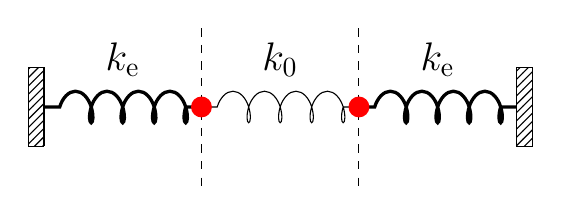
\begin{tikzpicture}
				\filldraw[pattern=north east lines] (0,-0.5) -| (-0.2,0.5) -| (0,-0.5);
				\filldraw[pattern=north east lines] (6,-0.5) -| (6.2,0.5) -| (6,-0.5);
				\draw[Spring] (0,0) -- (2,0);
				\draw[Spring, thin] (2,0) -- (4,0);
				\draw[Spring] (4,0) -- (6,0);
				
				\draw [dashed] (2,1) -- (2,-1);
				\draw [dashed] (4,1) -- (4,-1);
				
				\draw (2,0) node [fill=red,circle,scale=0.8] {};
				\draw (4,0) node [fill=red,circle,scale=0.8] {};
				
				\Large
				\draw (1,0.6) node [] {$k_\textrm{e}$};
				\draw (3,0.6) node [] {$k_0$};
				\draw (5,0.6) node [] {$k_\textrm{e}$};
			\end{tikzpicture}
			\label{fig: springs sym eq}}}

		\subfloat[Symmetric sloshing]{\scalebox{0.6}{
			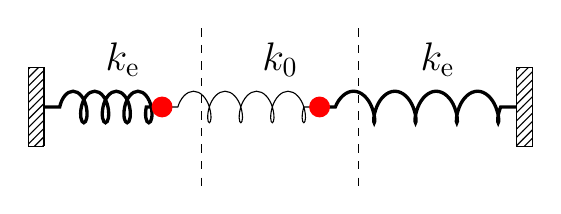
\begin{tikzpicture}
				\filldraw[pattern=north east lines] (0,-0.5) -| (-0.2,0.5) -| (0,-0.5);
				\filldraw[pattern=north east lines] (6,-0.5) -| (6.2,0.5) -| (6,-0.5);
				\draw[Spring] (0,0) -- (1.5,0);
				\draw[Spring, thin] (1.5,0) -- (3.5,0);
				\draw[Spring] (3.5,0) -- (6,0);
				
				\draw [dashed] (2,1) -- (2,-1);
				\draw [dashed] (4,1) -- (4,-1);
				
				\draw (1.5,0) node [fill=red,circle,scale=0.8] {};
				\draw (3.5,0) node [fill=red,circle,scale=0.8] {};
				
				\Large
				\draw (1,0.6) node [] {$k_\textrm{e}$};
				\draw (3,0.6) node [] {$k_0$};
				\draw (5,0.6) node [] {$k_\textrm{e}$};
			\end{tikzpicture}
			\label{fig: springs sym in-phase}}}

		\subfloat[Symmetric breathing]{\scalebox{0.6}{
			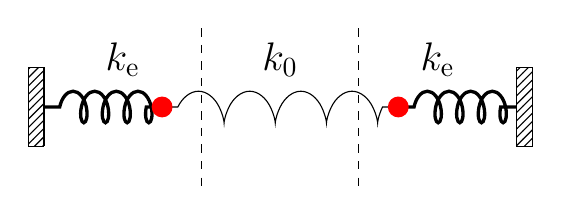
\begin{tikzpicture}
				\filldraw[pattern=north east lines] (0,-0.5) -| (-0.2,0.5) -| (0,-0.5);
				\filldraw[pattern=north east lines] (6,-0.5) -| (6.2,0.5) -| (6,-0.5);
				\draw[Spring] (0,0) -- (1.5,0);
				\draw[Spring, thin] (1.5,0) -- (4.5,0);
				\draw[Spring] (4.5,0) -- (6,0);
				
				\draw [dashed] (2,1) -- (2,-1);
				\draw [dashed] (4,1) -- (4,-1);
				
				\draw (1.5,0) node [fill=red,circle,scale=0.8] {};
				\draw (4.5,0) node [fill=red,circle,scale=0.8] {};
				
				\Large
				\draw (1,0.6) node [] {$k_\textrm{e}$};
				\draw (3,0.6) node [] {$k_0$};
				\draw (5,0.6) node [] {$k_\textrm{e}$};
			\end{tikzpicture}
			\label{fig: springs sym anti-phase}}}}
	\\
	\makebox[\textwidth][c]{
		\subfloat[Asymmetric equilibrium]{\scalebox{0.6}{
			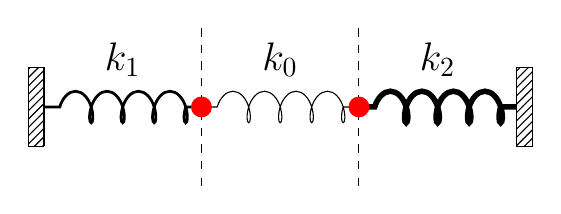
\begin{tikzpicture}
				\filldraw[pattern=north east lines] (0,-0.5) -| (-0.2,0.5) -| (0,-0.5);
				\filldraw[pattern=north east lines] (6,-0.5) -| (6.2,0.5) -| (6,-0.5);
				\draw[Spring, line width=1] (0,0) -- (2,0);
				\draw[Spring, thin] (2,0) -- (4,0);
				\draw[Spring, line width=2] (4,0) -- (6,0);
				
				\draw [dashed] (2,1) -- (2,-1);
				\draw [dashed] (4,1) -- (4,-1);
				
				\draw (2,0) node [fill=red,circle,scale=0.8] {};
				\draw (4,0) node [fill=red,circle,scale=0.8] {};
				
				\Large
				\draw (1,0.6) node [] {$k_1$};
				\draw (3,0.6) node [] {$k_0$};
				\draw (5,0.6) node [] {$k_2$};
			\end{tikzpicture}
			\label{fig: springs asym eq}}}

		\subfloat[Asymmetric sloshing]{\scalebox{0.6}{
			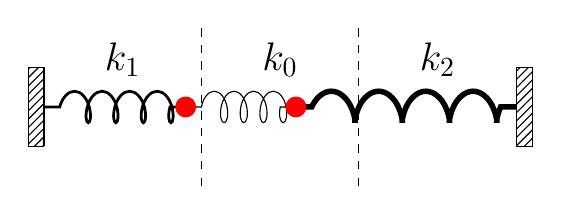
\begin{tikzpicture}
				\filldraw[pattern=north east lines] (0,-0.5) -| (-0.2,0.5) -| (0,-0.5);
				\filldraw[pattern=north east lines] (6,-0.5) -| (6.2,0.5) -| (6,-0.5);
				\draw[Spring, line width=1] (0,0) -- (1.8,0);
				\draw[Spring, thin] (1.8,0) -- (3.2,0);
				\draw[Spring, line width=2] (3.2,0) -- (6,0);
				
				\draw [dashed] (2,1) -- (2,-1);
				\draw [dashed] (4,1) -- (4,-1);
				
				\draw (1.8,0) node [fill=red,circle,scale=0.8] {};
				\draw (3.2,0) node [fill=red,circle,scale=0.8] {};
				
				\Large
				\draw (1,0.6) node [] {$k_1$};
				\draw (3,0.6) node [] {$k_0$};
				\draw (5,0.6) node [] {$k_2$};
			\end{tikzpicture}
			\label{fig: springs asym in-phase}}}

		\subfloat[Asymmetric breathing]{\scalebox{0.6}{
			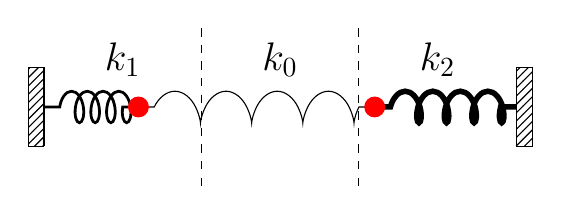
\begin{tikzpicture}
				\filldraw[pattern=north east lines] (0,-0.5) -| (-0.2,0.5) -| (0,-0.5);
				\filldraw[pattern=north east lines] (6,-0.5) -| (6.2,0.5) -| (6,-0.5);
				\draw[Spring, line width=1] (0,0) -- (1.2,0);
				\draw[Spring, thin] (1.2,0) -- (4.2,0);
				\draw[Spring, line width=2] (4.2,0) -- (6,0);
				
				\draw [dashed] (2,1) -- (2,-1);
				\draw [dashed] (4,1) -- (4,-1);
				
				\draw (1.2,0) node [fill=red,circle,scale=0.8] {};
				\draw (4.2,0) node [fill=red,circle,scale=0.8] {};
				
				\Large
				\draw (1,0.6) node [] {$k_1$};
				\draw (3,0.6) node [] {$k_0$};
				\draw (5,0.6) node [] {$k_2$};
			\end{tikzpicture}
			\label{fig: springs asym anti-phase}}}}

	\caption{A coupled mechanical oscillator gives an analogy to the eigenmodes of symmetric and asymmetric magnetic slabs. Spring constants are denoted $k$, with a thicker spring corresponding to a higher spring constant. Figures~(a) and~(d) show the symmetric and asymmetric spring systems in equilibrium. Figures~(b) and~(c) show the normal modes of a symmetric system. Figures~(e) and~(f) show the normal modes of an asymmetric system with spring constants $k_2 > k_1$. In each panel, the vertical dashed lines give the positions of the red masses at equilibrium.}
	\label{fig: springs all}
\end{figure}


%------------------------------------------------------------------------------
\section{Asymmetric slab in a magnetic environment}
\label{sec: EVP mag}
%------------------------------------------------------------------------------

Now we return to the general model for a magnetic slab, that is, a magnetic slab with asymmetric external environment.

\subsection{Summary of the eigenmode}

The eigenmodes and their dispersion is broadly similar to the slab in a non-magnetic environment. The differences, where they exist, are briefly discussed here.

\begin{figure}[]
	\centering
	\subfloat[$v_{A0} > c_0$]{\includegraphics[scale=0.45]{\figdir disp-mag-outside-photophere.png}
		\label{fig: disp mag 1}}
	\subfloat[$v_{A0} < c_0$]{\includegraphics[scale=0.45]{\figdir disp-mag-outside-2.png}
		\label{fig: disp mag 2}}
	\caption{Dispersion diagram for the dispersion relation, Equation~\eqref{DR}. \textcolor{red}{Finish}}
	\label{fig: disp mag}
\end{figure}


\subsection{Implications for observations}

Accurate mode identification is a key aspect of SMS. Different modes can differ in characteristics such as damping rate, phase and group speed, and, most relevant to this Thesis, response to waveguide asymmetry. Therefore, inaccurate mode identification can lead to significant error in diagnosis of background parameters. This subsection warns observational solar physicists of two possible ways in which errors in mode identification  could be made due to waveguide asymmetry.


\subsubsection{Quasi-symmetric eigenmodes}

It is possible for asymmetric MHD waves to have similar observational qualities to symmetric MHD waves. This can occur when the restoring force of perturbations (that is, the sum of the pressure gradient and Lorentz forces) is equal at both interfaces. This can occur in an asymmetric slab when the asymmetry in the pressure gradient force is precisely balanced to the asymmetry in the Lorentz force. We define these as \textit{quasi-symmetric} modes.

More precisely, we define quasi-symmetric modes to be eigenmodes which have equal transverse displacement amplitude on each boundary of the slab. This is equivalent to setting $\hat{v}_x (-x_0) = - \hat{v}_x (x_0)$ for quasi-sausage modes and $\hat{v}_x (-x_0) = \hat{v}_x (x_0)$ for quasi-kink modes.

The aim here is to prove that the necessary and sufficient condition for the existence of quasi-symmetric eigenmodes of an asymmetric magnetic slab is
\begin{equation}
\frac{\rho_1}{m_1}(k^2v_{A1}^2 - \omega^2) = \frac{\rho_2}{m_2}(k^2v_{A2}^2 - \omega^2), \label{quasi-sym condition}
\end{equation}
for a given frequency, $\omega$, and wavenumber, $k$.

To show that Equation~\eqref{quasi-sym condition} is sufficient for there to exist quasi-symmetric modes, consider an asymmetric magnetic slab with parameters that satisfy Equation~\eqref{quasi-sym condition}. Under this supposition, the transverse velocity perturbation solution for quasi-sausage modes reduces to
\begin{equation}
\hat{v}_x(x) =
\begin{cases}
A(\cosh{m_1x} + \sinh{m_1x}) & \text{if } x < -x_0, \\
C\sinh{m_0x} & \text{if } |x| \leq x_0, \\
D(\cosh{m_2x} - \sinh{m_2x}) & \text{if  } x > x_0,
\end{cases}
\end{equation}
where
\begin{equation}
A = \frac{-Cs_0}{c_1 - s_1}, \quad
D = \frac{Cs_0}{c_2 - s_2}, \quad
C \text{ is arbitrary}.
\end{equation}
The solution within the slab, $|x| \leq x_0$, is an odd function of $x$, therefore $\hat{v}_x(x_0) = -\hat{v}_x(-x_0)$. Therefore Equation~\eqref{quasi-sym condition} is a sufficient condition for the existence of quasi-symmetric modes. For quasi-kink modes, a similar proof is followed, where we find that $\hat{v}_x(x)$ is an even function within the slab.

To show that Equation~\eqref{quasi-sym condition} is necessary for there to exist quasi-symmetric modes, consider an asymmetric magnetic slab which supports quasi-symmetric modes. The transverse velocity perturbation solution is given by
\begin{equation}
\hat{v}_x(x) =
\begin{cases}
A(\cosh{m_1x} + \sinh{m_1x}) & \text{if } x < -x_0, \\
B\cosh{m_0x} + C\sinh{m_0x} & \text{if } |x| \leq x_0, \\
D(\cosh{m_2x} - \sinh{m_2x}) & \text{if } x > x_0, \label{vsoln}
\end{cases}
\end{equation}
where
\begin{align}
A &= \frac{1}{c_1 - s_1}(Bc_0 - Cs_0), \label{constA C} \\ 
D &= \frac{1}{c_2 - s_2}(Bc_0 + Cs_0), \label{constD C} \\
B &= \frac{\Lambda_0c_0 + \Lambda_1s_0}{\Lambda_0s_0 + \Lambda_1c_0}C = -\frac{\Lambda_0c_0 + \Lambda_2s_0}{\Lambda_0s_0 + \Lambda_2c_0}C, \label{constB C} \\
C & \text{ is arbitrary},
\end{align}
for quasi-sausage modes, and
\begin{align}
A &= \frac{1}{c_1 - s_1}(Bc_0 - Cs_0), \label{constA B} \\ 
D &= \frac{1}{c_2 - s_2}(Bc_0 + Cs_0), \label{constD B} \\
C &= \frac{\Lambda_0s_0 + \Lambda_1c_0}{\Lambda_0c_0 + \Lambda_1s_0}B = -\frac{\Lambda_0s_0 + \Lambda_2c_0}{\Lambda_0c_0 + \Lambda_2s_0}B, \label{constB B} \\
B & \text{ is arbitrary},
\end{align}
for quasi-kink modes. Given the supposition that the slab supports quasi-symmetric modes, we have, for quasi-sausage modes,
\begin{align}
\hat{v}_x(-x_0) &= -\hat{v}_x(x_0), \\
\implies \left(\frac{\Lambda_0c_0 + \Lambda_1s_0}{\Lambda_0s_0 + \Lambda_1c_0}\right) c_0 - s_0 &= -\left(\frac{\Lambda_0c_0 + \Lambda_1s_0}{\Lambda_0s_0 + \Lambda_1c_0}\right)c_0 - s_0, \\
\implies \Lambda_0c_0 + \Lambda_1s_0 &= 0.
\end{align}
Similarly, taking the second expression for $B$, we deduce that 
\begin{equation}
\Lambda_0c_0 + \Lambda_2s_0 = 0.
\end{equation}
It follows that $\Lambda_1 = \Lambda_2$, which is equivalent to Equation~\eqref{quasi-sym condition}, which concludes the proof that it is a necessary condition for the existence of quasi-symmetric quasi-sausage modes. For quasi-kink modes, a similar proof can be followed to show that $\hat{v}_x(x_0) = \hat{v}_x(-x_0)$ implies Equation~\eqref{quasi-sym condition}.






If we further specify that the penetration depth of perturbations in the external plasma be equal on each side of the slab, so that the eigenfunction is fully symmetric, then this implies that the external parameters are equal and we have a symmetric slab.

The main corollary to this result is that one can not conclude from an observation of a symmetric-looking MHD wave that the underlying waveguide is symmetric. This fallacy has been made in a number of previous studies (CITE) and could have lead to incorrect mode identification or diagnosis of the background plasma.

The question is then this: \textit{is it possible to differentiate between a symmetric and a quasi-symmetric eigenmode?} The answer to this is unclear. Theoretically, the answer is \textit{yes}. Although quasi-symmetric modes have symmetric amplitudes at the boundaries, they have asymmetric penetration depths into the external plasmas \textcolor{red}{(consider making a figure to show this in python)}. In theory, one could track the attenuation of the oscillation amplitude of plasma further away from the slab on each side. If the attenuation is asymmetric, the mode is quasi-symmetric. In practice, however, this will prove difficult. Although we currently have the required spatial resolution for measuring the spatial attenuation of MHD waves in many solar waveguides, the waveguides are unlikely to be isolated enough to allow for good measurements of this.


\subsubsection{Asymmetric mode or superposition of symmetric modes?}

A second implication that asymmetric eigenmodes have on mode identification in solar observations is that a waveguide oscillating in an asymmetric mode could be indistinguishable from a superposition of symmetric eigenmodes.

Consider how one has traditionally identified sausage and kink eigenmodes of a symmetric waveguide. To identify sausage modes, it has been presumed sufficient to identify oscillation in the cross-sectional width. To identify kink modes, it has been presumed sufficient to identify oscillation in the waveguide axis \textcolor{red}{(CITE?)}. The mixed characteristics of sausage and kink modes in asymmetric waveguides (see Table~\ref{tab: eigenmode differences}) tell us that these two characteristics are \textit{necessary} but not \textit{sufficient} for identification of the respective modes.

To appreciate the potential misidentification, consider a hypothetical observation of a waveguide in the solar atmosphere from which oscillations can be identified in both the cross-sectional width and the axis (for example, Figure~\ref{}, which uses the same dataset analysed by \cite{mor_etal12}). If the oscillation is linear, the naive approach is to assume that the waveguide is symmetric, so that the only explanation for the cross-sectional oscillation is a symmetric sausage mode and the only explanation for the axial oscillation is a symmetric kink mode. One might then conclude that the observation is of a superposition of a sausage mode and a kink mode. However, 

One possible resolution to this problem is to measure the background parameters on each side of the waveguide to determine the degree of asymmetry before identifying the modes. If the waveguide is determined to be symmetric, symmetric modes can be identified. If not, the more general asymmetric modes can be identified.

One problem with this approach is that determining the key background parameters, the density and magnetic field strength, is often very difficult and estimates will have an associated uncertainty large enough that it would often not be possible to rule out the possibility of asymmetry. Another problem with this approach is that even relatively small degrees of waveguide asymmetry can cause significant asymmetry in the eigenmodes. For example, Figure~\ref{} gives a case where the ratio of the external densities is only \textcolor{red}{<CHANGE ME>}, yet the asymmetry in the eigenmodes (measured for example by the ratio of the oscillation amplitudes at each interface) is sufficient to show up in observations.

A second resolution is to independently measure the propagation speeds of the cross-sectional width oscillation and axial oscillation. Distinct eigenmodes propagate at distinct phase speeds\footnote{This is because of the uniqueness of eigenvalues in Sturm-Liouville systems \citep{boy_etal12}.}. If, in fact, the observation is of a superposition of symmetric sausage and kink eigenmodes, then each eigenmode will propagate at a distinct phase speed. Specifically, the cross-sectional oscillation will propagate at a different speed to the axial oscillation, and the oscillations will become out of phase. Whereas, if the oscillations in cross-sectional width and axis are both due to a single asymmetric eigenmode, then they will both share the same propagation speed and remain in phase. If different propagation speeds between these oscillation can be identified, then it will more likely be a superposition of symmetric modes than asymmetric modes.

One problem with this approach is that often only a small number of periods are observed before either the wave is damped or the waveguide disappears from observational view or breaks up. A notable exception to this are decayless kink oscillations \citep{nis_etal13}. When only a small number of periods are observed, there are often either too few periods to observe the cross-sectional width oscillations to become out of phase with axial oscillations, or errors in the phase-speed measurements too large to determine a difference. A second problem is that for some equilibrium parameters, the phase speeds of the symmetric sausage and kink eigenmodes are very similar. For example, this is true for body modes in most parameter regimes and for surface modes in a wide slab (Figure~\ref{} \textcolor{red}{Include a figure of symmetric slab dispersion diagrams}).

\color{red}


%------------------------------------------------------------------------------
\section{Other asymmetric waveguides}
\label{sec: other waveguides}
%------------------------------------------------------------------------------

For completion, we briefly discuss other studies of MHD waveguides that display asymmetric properties. 

\subsection{Multi-layered plasma}
\cite{rud92}
\cite{all_etal19}


\subsection{Adjacent waveguides}

\subsection{Non-axisymmetric magnetic flux-tubes}
Elliptical cross section
\cite{gu_etal80}
\cite{erd_etal09}
\cite{rud03}
\cite{mor_etal11}





%------------------------------------------------------------------------------
\section{Chapter conclusions}
\label{sec: chpt 2 conc}
%------------------------------------------------------------------------------
\color{black}


\appendix
\section{Coupled oscillator asymmetric eigenmodes} \label{app: coupled oscillator modes}
In this appendix, we prove that the breathing mode has highest amplitude on the mass connected to the external spring with lowest spring constant and the sloshing mode has highest amplitude on the mass connected to the external spring with highest spring constant.

Without loss of generality, let $\omega_2 > \omega_1$, so that the spring on the right has higher spring constant than the spring on the left. First, consider the case when $W < 1$. For the breathing mode, which has eigenfrequency $\omega_+$,
\begin{align}
	\left| \frac{\hat{x}_1}{\hat{x}_2} \right| & = \frac{1}{2W} \left(1 + \sqrt{1 + 4W^2}\right) \\
	& >  \frac{1}{2} \left(1 + \sqrt{1}\right), \quad \text{since $0 < W < 1$,} \\
	& = 1.
\end{align}
Therefore, the oscillation amplitude of the mass on the left is higher. For the sloshing mode, which has eigenfrequency $\omega_-$,
\begin{align}
	\left| \frac{\hat{x}_1}{\hat{x}_2} \right| & = \frac{1}{2W} \left|1 - \sqrt{1 + 4W^2}\right| \\
	& = \frac{1}{2W} \left(\sqrt{1 + 4W^2} - 1\right) \\
	& \leq \frac{1}{2W} \left(\sqrt{1} + \sqrt{4W^2} - 1\right), \quad \text{by the triangle inequality,} \\
	& = 1.
\end{align}
Therefore, the oscillation amplitude of the mass on the right is higher.

Next, consider the case when $W > 1$. For the breathing mode,
\begin{align}
\left| \frac{\hat{x}_1}{\hat{x}_2} \right| & = \frac{1}{2W} \left(1 + \sqrt{1 + 4W^2}\right) \\
& \geq \frac{1}{2W} \sqrt{2 + 4W^2}, \quad \text{by the triangle inequality,} \\
& = \sqrt{\frac{1}{2W} + 1} \\
& > 1,  \quad \text{since $W > 0$.}
\end{align}
Therefore, the oscillation amplitude of the mass on the left is higher. For the sloshing mode,
\begin{align}
\left| \frac{\hat{x}_1}{\hat{x}_2} \right| & = \frac{1}{2W} \left(\sqrt{1 + 4W^2} - 1\right) \\
& \leq \frac{1}{2W} \left(\sqrt{1 + 4W^2 - 1}\right), \quad \text{by the reverse triangle inequality,} \\
& = 1.
\end{align}
Therefore, the oscillation amplitude of the mass on the right is higher.

Finally, it is trivial to show the same result holds in the case where $W = 1$. This completes the proof that the breathing mode has highest amplitude on the mass connected to the external spring with lowest spring constant and the sloshing mode has highest amplitude on the mass connected to the external spring with highest spring constant.


\bibliographystyle{agsm}
\bibliography{../main/references}  

\end{document}

\documentclass[12pt]{../style-files/ociamthesis}
 
\usepackage{amssymb}
\usepackage{titlesec}
\usepackage{amsmath}
\usepackage{float}
\usepackage{graphicx}
\usepackage{caption}
\usepackage{subfig}
\usepackage{xcolor}
\usepackage[section]{placeins}
\usepackage{mathrsfs}
\usepackage{bm}
\usepackage{stmaryrd}
\usepackage{siunitx}
\usepackage{rotating}
\usepackage[utf8]{inputenc}
\usepackage[round]{natbib}

\usepackage{geometry}
 \geometry{
 a4paper,
 left=40mm,
 right=30mm,
 top=30mm,
 bottom=30mm
 }

\definecolor{theblue}{HTML}{0000CD}

% disable this package for printed version
\usepackage[colorlinks=true, linktocpage=true, allcolors=theblue]{hyperref}

\titleformat{\chapter}[display]
  {\bfseries\Large}
  {\filright\MakeUppercase{\chaptertitlename} \Large\thechapter}
  {1ex}
  {}
  [\vspace{1ex} \hrule \vspace{1pt} \hrule]

\newcommand{\adv}{    {\it Adv. Space Res.}} 
\newcommand{\annG}{   {\it Ann. Geophys.}} 
\newcommand{\aap}{    {\it Astron. Astrophys.}}
\newcommand{\aaps}{   {\it Astron. Astrophys. Suppl.}}
\newcommand{\aapr}{   {\it Astron. Astrophys. Rev.}}
\newcommand{\ag}{     {\it Ann. Geophys.}}
\newcommand{\aj}{     {\it Astron. J.}} 
\newcommand{\apj}{    {\it Astrophys. J.}}
\newcommand{\apjl}{   {\it Astrophys. J. Lett.}}
\newcommand{\apss}{   {\it Astrophys. Space Sci.}} 
\newcommand{\cjaa}{   {\it Chin. J. Astron. Astrophys.}} 
\newcommand{\gafd}{   {\it Geophys. Astrophys. Fluid Dyn.}}
\newcommand{\grl}{    {\it Geophys. Res. Lett.}}
\newcommand{\ijga}{   {\it Int. J. Geomagn. Aeron.}}
\newcommand{\jastp}{  {\it J. Atmos. Solar-Terr. Phys.}} 
\newcommand{\jgr}{    {\it J. Geophys. Res.}}
\newcommand{\mnras}{  {\it Mon. Not. Roy. Astron. Soc.}}
\newcommand{\na}{     {\it New Astronomy}}
\newcommand{\nat}{    {\it Nature}}
\newcommand{\pasp}{   {\it Pub. Astron. Soc. Pac.}}
\newcommand{\pasj}{   {\it Pub. Astron. Soc. Japan}}
\newcommand{\pre}{    {\it Phys. Rev. E}}
\newcommand{\solphys}{{\it Solar Phys.}}
\newcommand{\sovast}{ {\it Soviet  Astron.}} 
\newcommand{\ssr}{    {\it Space Sci. Rev.}}
\newcommand{\caa}{    {\it Chinese Astron. Astrohpys.}} 
\newcommand{\apjs}{   {\it Astrophys. J. Suppl.}}

\begin{document}

\baselineskip=18pt

\setcounter{secnumdepth}{3}
\setcounter{tocdepth}{3}

\setcounter{chapter}{2}


%------------------------------------------------------------------------------
\chapter{Asymmetric waveguides - initial value problem}
\label{chap: IVP}
%------------------------------------------------------------------------------

%------------------------------------------------------------------------------
\section{Chapter introduction}
\label{sec: IVP intro}
%------------------------------------------------------------------------------

%------------------------------------------------------------------------------
\section{Interface plasma}
\label{sec: IVP int}
%------------------------------------------------------------------------------

%------------------------------------------------------------------------------
\section{Asymmetric slab}
\label{sec: IVP slab}
%------------------------------------------------------------------------------


\bibliographystyle{agsm}
\bibliography{../main/references}

\end{document}

\documentclass[12pt]{../style-files/ociamthesis}
 
\usepackage{amssymb}
\usepackage{titlesec}
\usepackage{amsmath}
\usepackage{float}
\usepackage{graphicx}
\usepackage{caption}
\usepackage{subfig}
\usepackage{xcolor}
\usepackage[section]{placeins}
\usepackage{mathrsfs}
\usepackage{bm}
\usepackage{stmaryrd}
\usepackage{siunitx}
\usepackage{rotating}
\usepackage[utf8]{inputenc}
\usepackage[round]{natbib}
\usepackage{tikz}
\usetikzlibrary{fadings}
\usetikzlibrary{arrows,shapes, positioning}
\usepackage{booktabs}
\usepackage{multirow}
\usepackage{rotating}

%%%%%%%%%%%%%%%%%%%%%%%%%%%%%%%%%%%%%%%%%%%%%%%%%%%%%%%%%%%%%%%%%%%%%%%
% the following is to alter tikz settings to improve springs figure.
\usetikzlibrary{decorations.pathmorphing,calc,patterns}
\makeatletter
\def\pgfdecorationspringstraightlinelength{0.5cm}
\def\pgfdecorationspringnumberofelement{8}
\def\pgfdecorationspringnaturallength{5cm}
\pgfkeys{%
	/pgf/decoration/.cd,
	spring straight line length/.code={%
		\pgfmathsetlengthmacro\pgfdecorationspringstraightlinelength{#1}},
	spring natural length/.code={%
		\pgfmathsetlengthmacro\pgfdecorationspringnaturallength{#1}},
	spring number of element/.store in=\pgfdecorationspringnumberofelement
}

\pgfdeclaredecoration{coil spring}{straight line}{%
	\state{straight line}[%
	persistent precomputation = {%
		% Compute the effective length of the spring (without the length
		% of the two straight lines): \pgfdecorationspringeffectivelength
		\pgfmathsetlengthmacro{\pgfdecorationspringeffectivelength}%
		{\pgfdecoratedpathlength-2*\pgfdecorationspringstraightlinelength}
		% Compute the effective length of one coil pattern:
		% \pgfdecorationspringeffectivelengthofonecoil
		\pgfmathsetlengthmacro{\pgfdecorationspringeffectivelengthofonecoil}%
		{\pgfdecorationspringeffectivelength/\pgfdecorationspringnumberofelement}
	},
	width = \pgfdecorationspringstraightlinelength,
	next state = draw spring]{%
		\pgfpathlineto{%
			\pgfqpoint{%
				\pgfdecorationspringstraightlinelength}{0pt}}
	}
	\state{draw spring}%
	[width=\pgfdecorationspringeffectivelengthofonecoil,
	repeat state=\pgfdecorationspringnumberofelement-1,next state=final]{%
		\pgfpathcurveto
		{\pgfpoint@onspringcoil{0    }{ 0.555}{1}}
		{\pgfpoint@onspringcoil{0.445}{ 1    }{2}}
		{\pgfpoint@onspringcoil{1    }{ 1    }{3}}
		\pgfpathcurveto
		{\pgfpoint@onspringcoil{1.555}{ 1    }{4}}
		{\pgfpoint@onspringcoil{2    }{ 0.555}{5}}
		{\pgfpoint@onspringcoil{2    }{ 0    }{6}}
		\pgfpathcurveto
		{\pgfpoint@onspringcoil{2    }{-0.555}{7}}
		{\pgfpoint@onspringcoil{1.555}{-1    }{8}}
		{\pgfpoint@onspringcoil{1    }{-1    }{9}}
		\pgfpathcurveto
		{\pgfpoint@onspringcoil{0.445}{-1    }{10}}
		{\pgfpoint@onspringcoil{0    }{-0.555}{11}}
		{\pgfpoint@onspringcoil{0    }{ 0    }{12}}
	}
	\state{final}{%
		\pgfpathlineto{\pgfpointdecoratedpathlast}
	}
}

\def\pgfpoint@onspringcoil#1#2#3{%
	\pgf@x=#1\pgfdecorationsegmentamplitude%
	\pgf@x=.5\pgf@x%
	\pgf@y=#2\pgfdecorationsegmentamplitude%
	\pgfmathparse{0.083333333333*\pgfdecorationspringeffectivelengthofonecoil}%
	\pgf@xa=\pgfmathresult pt
	\advance\pgf@x by#3\pgf@xa%
}

\makeatother

\tikzset{%
	Spring/.style = {%
		decoration = {%
			coil spring,
			spring straight line length = 0.2cm,
			% To be added
			spring natural length = #1,
			spring number of element = 4,
			amplitude=2mm},
		decorate,
		very thick},
	Spring/.default = {4cm}}
%
%%%%%%%%%%%%%%%%%%%%%%%%%%%%%%%%%%%%%%%%%%%%%%%%%%%%%%%%%%%%%%%%%%%%%%%%%%%%%%%%

\usepackage{geometry}
 \geometry{
 a4paper,
 left=40mm,
 right=30mm,
 top=30mm,
 bottom=30mm
 }

\definecolor{theblue}{HTML}{0000CD}

% disable this package for printed version
\usepackage[colorlinks=true, linktocpage=true, allcolors=theblue]{hyperref}

\titleformat{\chapter}[display]
  {\bfseries\Large}
  {\filright\MakeUppercase{\chaptertitlename} \Large\thechapter}
  {1ex}
  {}
  [\vspace{1ex} \hrule \vspace{1pt} \hrule]

\newcommand{\adv}{    {\it Adv. Space Res.}} 
\newcommand{\annG}{   {\it Ann. Geophys.}} 
\newcommand{\aap}{    {\it Astron. Astrophys.}}
\newcommand{\aaps}{   {\it Astron. Astrophys. Suppl.}}
\newcommand{\aapr}{   {\it Astron. Astrophys. Rev.}}
\newcommand{\ag}{     {\it Ann. Geophys.}}
\newcommand{\aj}{     {\it Astron. J.}} 
\newcommand{\apj}{    {\it Astrophys. J.}}
\newcommand{\apjl}{   {\it Astrophys. J. Lett.}}
\newcommand{\apss}{   {\it Astrophys. Space Sci.}} 
\newcommand{\cjaa}{   {\it Chin. J. Astron. Astrophys.}} 
\newcommand{\gafd}{   {\it Geophys. Astrophys. Fluid Dyn.}}
\newcommand{\grl}{    {\it Geophys. Res. Lett.}}
\newcommand{\ijga}{   {\it Int. J. Geomagn. Aeron.}}
\newcommand{\jastp}{  {\it J. Atmos. Solar-Terr. Phys.}} 
\newcommand{\jgr}{    {\it J. Geophys. Res.}}
\newcommand{\mnras}{  {\it Mon. Not. Roy. Astron. Soc.}}
\newcommand{\na}{     {\it New Astronomy}}
\newcommand{\nat}{    {\it Nature}}
\newcommand{\pasp}{   {\it Pub. Astron. Soc. Pac.}}
\newcommand{\pasj}{   {\it Pub. Astron. Soc. Japan}}
\newcommand{\pre}{    {\it Phys. Rev. E}}
\newcommand{\solphys}{{\it Solar Phys.}}
\newcommand{\sovast}{ {\it Soviet  Astron.}} 
\newcommand{\ssr}{    {\it Space Sci. Rev.}}
\newcommand{\caa}{    {\it Chinese Astron. Astrohpys.}} 
\newcommand{\apjs}{   {\it Astrophys. J. Suppl.}}
\newcommand{\lrsp}{{\it Living Rev. Solar Phys.}}

\newcommand{\bv}{\mathbf{v}}
\newcommand{\bB}{\mathbf{B}}

\newcommand{\figdir}{../main/figures/chpt-4/} % where figures are stored


\begin{document}

\baselineskip=18pt

\setcounter{secnumdepth}{3}
\setcounter{tocdepth}{3}

\setcounter{chapter}{3}


%------------------------------------------------------------------------------
\chapter{Asymmetric waveguides - solar magneto-seismology}
\label{chap: SMS}
%------------------------------------------------------------------------------

%------------------------------------------------------------------------------
\section{Chapter introduction}
\label{sec: SMS intro}
%------------------------------------------------------------------------------

\color{red}{(STRAIGHT FROM THE INTRO OF ALL + ERD 2018 - PLZ CHANGE)The emerging field of solar magneto-seismology (SMS) has become a crucial tool in developing our understanding of structures in the solar atmosphere. By comparing observational measurements of magnetohydrodynamic (MHD) waves to the wave solutions of inhomogeneous plasma modelling of the medium in which the waves propagate, we can make approximations of traditionally difficult-to-measure plasma parameters such as the magnetic field strength and heat transport coefficient \citep{and_etal09,arr12,dem_etal12}. This in turn equips us with more realistic parameters for numerical simulations and give us a better understanding of conditions that lead to, for example, wave energy dissipation, instability, magnetic reconnection, and heating.

SMS techniques can be categorised as either temporal or spatial seismology. By temporal seismology we refer to methods that estimate a plasma parameter by using the observed frequency, or equivalently the period, of waves. By spatial seismology we refer to methods that estimate a plasma parameter by comparing the observed spatial and/or temporal wave power distribution with the eigenfunctions from a theoretical model.

Several temporal seismology methods have been employed successfully. \cite{ros70} first suggested that the frequency of oscillations, observed through the fluctuation of synchrotron radiation due to the presence of MHD waves, could be used to diagnose background parameters. Further theoretical development has led to more sophisticated temporal methods including local coronal magnetic field strength estimates using standing kink modes in coronal loops by \cite{nak_etal01}, and using slow sausage and kink modes by \cite{erd_etal08}. The ratio of periods of the fundamental and the first harmonic standing kink mode and its dependence on density stratification has also been well studied \citep{ban_etal07,erd_etal14,yu_etal16}.

Spatial seismology techniques have more recently started demonstrating their efficacy in estimating solar parameters. \cite{uch70} estimated the coronal magnetic structure by comparing Moreton wave observations with the theoretical influence that the coronal magnetic field has on the shape of the Moreton wavefront. More recent eigenfunction methods include utilising the anti-node shift of standing modes in a magnetic flux tube to diagnose its inhomogeneous density stratification \citep{erd_etal07,ver_etal07,erd_etal14}.

In the present work, we derive two novel analytical tools for spatial seismology that use an asymmetric slab waveguide to approximate background parameters. This has applications to solar atmospheric structures that are locally slab-like which have been observed to guide MHD oscillations, such as elongated magnetic bright points \citep{yua_etal14}, prominences \citep{arr_etal12}, and light bridge surges \citep{roy73,shi_etal09} (which have also been named light walls by, \textit{e.g.} \citealt{yan_etal15,yan_etal17,zha_etal17}).

This work provides an application of the linear wave analysis of asymmetric magnetic slabs completed by \cite{all_etal17}. A magnetic slab, with non-magnetic, but asymmetric density and temperatures outside the slab has eigenmodes which can be described as either quasi-sausage or quasi-kink. For quasi-sausage (quasi-kink) modes, the oscillations on each slab interface are in anti-phase (phase). They differ in character from traditional (symmetric) sausage and kink modes by their asymmetry about the center of the slab due to the amplitude of oscillation on each interface being unequal caused by the asymmetric external environment. This results in quasi-kink modes not necessarily retaining their cross-sectional area and quasi-sausage modes not necessarily having reflection symmetric about the centre line of the slab. The spatial distribution of these waves across the slab, and therefore the extent to which they are modified from the traditional sausage and kink modes, is dependent on the asymmetric background plasma parameters. Consequently, we can use the spatial distribution of these waves to diagnose the waveguide. This is the focus of the present paper: to derive expressions for proxy parameters that encapsulate this asymmetric spatial distribution and discuss the application to SMS.

Section~\ref{sec: AR} introduces the amplitude ratio diagnostic parameter, Section~\ref{sec: MPS} introduces the minimum perturbation shift diagnostic parameter, and Section~\ref{sec: discussion} discusses the application of these parameters to SMS.}
\color{black}


\subsection{What is solar magneto-seismology?}
As part of a broader set of magnetometry techniques.

\subsection{A brief history}








\textcolor{red}{All of below text needs editing (maybe shortening or putting in an appendix, too?)}
\subsection{Solar atmospheric magnetometry}
The magnetic field plays an integral role in the structure and dynamics of the solar atmosphere. Measuring the strength and direction of the magnetic field vector is therefore important for realistic numerical simulations and a better understanding of active magnetic structures on the Sun. (Maybe we could write more here about why it's important to understand magnetic field in the solar atmosphere)

The first magnetic field measurement techniques involved observing the effect that the field has on the electromagnetic radiation emitted from the plasma, so called \textit{spectral techniques}.

Later, indirect techniques, where we use a different observational proxy to diagnose the magnetic field information, were developed, including magnetic extrapolation and magneto-seismology. With increasing spatial and temporal resolution of solar observations, it is expected that these techniques will become more widely and accurately used.

A description of these techniques is given below.

\subsubsection{Spectral techniques}
\subsubsection{Zeeman effect}
The Zeeman effect is due to magnetic fields distorting the electron orbitals of atoms so that the wavelength of light emitted by electrons relaxing to lower energy levels is modified. This has the effect of splitting the emission lines of plasma in the presence of a magnetic field.

In solar observations, this effect was first observed in 1908 when George Ellery Hale noticed it in the H$\alpha$ spectrum from the 3000 G sunspot magnetic fields. Since then, the Zeeman effect has been the foremost employed solar magnetometry  technique. Since the Doppler broadening scales proportionally to the observed wavelength, $\lambda$, while the Zeeman splitting scales proportionally to $\lambda^2$, the different Zeeman components happen to be completely separated for sufficiently large values of $\lambda$. Infrared is often used to establish observations of Zeeman splitting for this reason.

It has been said that, with the Zeeman effect, “a ruler is sufficient to measure the solar magnetic field” \citep{lan03}. In some sense, this is true. The magnitude of the wavelength splitting of the emission lines is directly related to the strength of the magnetic field in the line-of-sight. To diagnose the direction of the magnetic field, polarimetry and radiative transfer are necessary in any wavelength observation.

Quantum effects must be considered to fully explain the nuances of the effect, in particular, the anomalous Zeeman effect which requires an appreciation of electron spin.

\subsubsection{Hanle effect}
The Hanle rotation effect is not dependent on the length of the path through the magnetic field (which makes it distinct from the Faraday effect). 

Quantum effects must be considered to fully explain the nuances of the effect.

\subsubsection{Indirect techniques}
\subsubsection{Faraday rotation}
When light passes through a magnetic field in a dispersive medium, the polarisation of the light is rotated proportionally to the strength of the magnetic field and the length of the path in the medium within the magnetic field. This is known as Faraday rotation. By observing light from a distant star of known polarisation as it passes through the rarefied solar corona and measuring the corresponding polarisation rotation, we can make an indirect measurement of the coronal magnetic field.

By observing the radiation from a background star with known radiation spectrum as it passes behind the outer corona, a measurement of the rotation of the polarisation of the light, and therefore a measurement of the line-of-sight magnetic field can be made.


\subsubsection{Photospheric extrapolation}
Currently, our measurements of the vector field in the $10^6$ K corona of the quiet Sun comes almost entirely from extrapolation of photospheric magnetic field measurements. The photospheric magnetic field (whose magnitude and direction can be measured with low uncertainty using observations of Zeeman splitting of spectral lines) is used as a lower boundary condition used to solve a set of differential equations for the magnetic field.

For quasi-stationary solar structures, such that the magnetostatic approximations is valid, balance between the Lorentz force, pressure gradient force, and gravity in the solar atmosphere can be written as
\begin{equation}
\mathbf{j} \times \mathbf{B} - \nabla p - \rho \mathbf{g} = 0.
\end{equation}
In the solar corona, the plasma is of low beta ($\beta \ll 1$), and for regions of vertical extent smaller than $H/\beta$, where $H$ is the pressure scale-height, the force balance simplifies to 
\begin{equation}
\mathbf{j} \times \mathbf{B} = 0,
\end{equation}
\textit{i.e.} the magnetic field is \textit{force-free}.

The simplest way to achieve a force-free magnetic field is to take $\mathbf{j} = 0$, describing a current-free (potential) field. For this simple type of field, there exists a magnetic scalar potential, $\phi = \phi(\mathbf{x})$, such that $\mathbf{B} = \nabla\phi$. Then, from the solenoidal condition, the scalar potential satisfies
\begin{equation}
\nabla^2 \phi = 0.
\end{equation}
This equation is solved using a Green's function method or an eigenfunction expansion method with the observed photospheric boundary condition to extrapolate the photospheric magnetic field into the corona.

A more sophisticated way to ensure a force-free magnetic field is to take the magnetic field parallel to the electric current, that is
\begin{equation}
\nabla \times \mathbf{B} = \alpha \mathbf{B},
\label{alpha1}
\end{equation}
where $\alpha$ is the proportionality between the magnetic field and the current. Taking the divergence of this equation gives us
\begin{equation}
\mathbf{B} \cdot \nabla\alpha = 0,
\label{alpha2}
\end{equation}
since $\nabla \cdot \mathbf{B} = 0$. From this, it follows that $\alpha$ is constant along each field line. When $\alpha$ is constant, the extrapolation is known as \textit{linear force-free}; if not, it is known as \textit{nonlinear force-free}.

The force-free equations (Equations~\eqref{alpha1} and~\eqref{alpha2}) must be solved numerically in all but the simplest of cases. Even when taking a simple upper-boundary condition that the magnetic field is negligible far from the solar surface, the problem is mathematically ill-posed (why?), in that a small change in the imposed photospheric boundary condition results in a large change in the extrapolated field \citep{low_etal90}. This is problematic due to the necessary uncertainty in the photospheric magnetic field measurements.


\subsubsection{Magneto-seismology}
Perpetual bubbling, erupting, and turbulent buffeting of plasma drive ubiquitous magneto-acoustic waves throughout the solar atmosphere. The topology and strength of the magnetic field determines the type  and their properties of waves present in a given structure. Therefore, by observing these waves and solving an inverse problem, it is possible to make a diagnosis of magnetic field information - a technique known as \textit{solar magneto-seismology} (SMS).

Since early observations of these waves were made in coronal loops at the end of the 20th century, further observations have shown their ubiquity across almost all magnetic structures in the solar atmosphere, including prominences, sunspots, fibrils, and light walls. This makes SMS a promising avenue for advancing our understanding of the coronal magnetic field.

Observations of MHD oscillations can give us both temporal and spatial parameters. For example, we can  
\newcommand{\tb}{\textcolor{black}}
\tikzstyle{format} = [draw, rounded corners=.055cm, fill=cyan!20]
\tikzstyle{format2} = [draw, rounded corners=.055cm, fill=red!20]
\begin{figure}
	\begin{tikzpicture}[node distance=1.8cm and 3.3cm, auto, >=latex, align = flush center, ultra thick, on grid=true, font=\small]
	% We need to set at bounding box first. Otherwise the diagram
	% will change position for each frame.
	\path[use as bounding box] (-1.7,-4.1) rectangle (10,2);
	\path node[format] (obs) {
		Observations};
	\path node[below= of obs] (ghost) {};
	\path node[format, below= of ghost] (phys) {
		Physical \\ 
		understanding};
	
	\path node[format2, below right= of obs] (ep) {
		Equilibrium \\ 
		parameters};
	\path (ep) edge[<-] (obs);
	\path node[format, above right= of obs] (wp) {
		Wave \\ 
		parameters}
	edge[<-] (obs);
	
	\path node[format, right= of wp] (tp) {
		Temporal \\ 
		parameters}
	edge[<-] (wp);
	\path node[format, below= of tp] (sp) {
		Spatial \\ 
		parameters}
	edge[<-] (wp)
	edge[<-] (ep);  
	
	\path node[format, right= of phys] (em) {
		Equilibrium \\ 
		models};
	\path (em) edge[<-] (phys);
	
	\path node[format, right= of em] (eig) {
		Eigenmodes}
	edge[<-] (em);
	
	\path node[format, right= of sp] (ts) {
		Temporal \\
		magneto-seismology};
	\path (ts) edge[<-] (tp);
	\node at (6.6,-2) (ghost2) {};
	\draw [->] (ghost2.center) -- (ts);
	\draw (ghost2.center) -- (eig);
	\path node[format, below right= of sp] (ss) {
		Spatial \\
		magneto-seismology};
	\draw [->] (eig) -- (ss);
	\path (ss) edge[<-] (sp);
	
	
	\path (ts) edge[->] (ep);
	\path (ss) edge[->] (ep);
	
	\end{tikzpicture}
	\caption{A flow chart describing the method of solar magneto-seismology.}
\end{figure}

Some of the major advancements in temporal magneto-seismology:
\begin{itemize}
	\item Rosenberg, 1970: Pulsations in synchrotron radiation caused by MHD waves,
	\item Zeitsev and Stepanov, 1975: Pulsations of type IV solar radio emission due to flux tube oscillations,
	\item Roberts et al., 1984: coronal seismology discussion,
	\item Tandberg Hanssen et al., 1995: Prominence seismology,
	\item Nakariakov and Ofman, 2001: Period of standing kink mode used to diagnose magnetic field strength,
	\item Goossens et al., 2002: Damping time scales (assuming exponential damping) used to estimate density variation across loop (?).
	\item Andries et al., 2005: Density stratification deduced from period ratio of first two standing kink harmonics,
	\item Erdelyi and Taroyan, 2008: Slow standing modes in loops,
	\item Pascoe et al., 2013: Gaussian and exponential damping of kink modes to estimate loop density,
	\item Magyar et al., 2017: Global dynamic coronal seismology - i.e. diagnosing the magnetic field strength changing in time and across a large portion of the corona.
\end{itemize}
Some of the major advancements in spatial magneto-seismology:
\begin{itemize}
	\item Uchida, 1970: Moreton wavefronts,
	\item Verth et al., 2007: Anti-node shift due to density stratification along the loop (e.g. higher density at food points).
\end{itemize}


\subsubsection{Future techniques}
\subsubsection{In-situ measurements}
NASA Parker Probe.

\subsection{Application and difficulties}
In the photosphere and chromosphere, the strength of both the line-of-sight and plane-of-sky magnetic field components (equivalently, the direction and magnitude of the magnetic field vector) can be made with low uncertainty using the Zeeman splitting of the spectral lines observed.

It is always difficult, and often impossible, to ascertain any magnetic field information in the corona. This is due to the fact that, although it dominates other forces involved, the magnetic field is of low absolute strength, and the plasma is extremely sparse. (WHY?)


\subsection{OTHER DETAILS TO ADD ABOVE}
From Aschwanden's book: "Above active regions, the magnetic field can sometimes be inferred from the change in sign and amplitude of the circular polarization when the microwave radiation passes through a quasi-transverse (QT) region (e.g., Ryabov et al. 1999). In weak-field regions far away from sunspots, the coronal field can also be probed by measuring the Faraday rotation (Alissandrakis  and Chiuderi-Drago 1995). Alternative methods to measure the coronal magnetic field have also been demonstrated by using the Fe XIII line in the infrared (Lin et al. 2000) or the Hanle effect (Stenflo 1994)."


\subsection{General techniques}
\subsubsection{Bayesian inversion}
Arregui and Asensio Ramos, 2011, developed a Bayesian scheme to reduce uncertainty in magnetic field measurements by giving accurate likelihood values on each solution from the multi-valued inversion procedure.


\subsection{Solar magneto-seismology using asymmetric waves}

\textcolor{red}{Lots of progress with temporal SMS, not much with spatial SMS. Prev sections show that if you change the background parameters, the asymmetry changes. Therefore, we can measure the asymmetry and invert the background parameters. How can we quantify this asymmetry? Amplitude ratio and minimum perturbation shift.}


%------------------------------------------------------------------------------
\section{Amplitude Ratio}
\label{sec: AR}
%------------------------------------------------------------------------------

The aim of this section is to derive an expression for the ratio of the oscillation amplitude on each interface of an asymmetric magnetic slab in terms of the wave parameters and plasma parameters of the system, then demonstrate how this parameter can be utilised to diagnose background parameters. We focus on estimating the Alfv\'{e}n speed since it is the the most difficult of all our background parameters to measure using traditional methods. We do this by first deriving expressions for the eigenfunctions\footnote{That is, the distribution of the oscillation amplitude across the waveguide.} of quasi-sausage and quasi-kink modes, using them to derive expressions for the Amplitude Ratio, and then by making suitable approximations, we can solve the inverse problem for the Alfv\'{e}n speed. Numerical inversion procedures for the Amplitude Ratio Method are discussed in Section~\ref{sec: numerical inversion} 

\subsection{Deriving an expression for the Amplitude Ratio} \label{sec: amp ratio}

Consider an asymmetric magnetic slab in a non-magnetic environment, as studied in Section~\ref{sec: EVP non-mag} and by \cite{all_etal17}. In this section, we denote the Alfv\'{e}n speed inside the slab as $v_\textrm{A}$ rather than $v_{A0}$ for brevity because it is the only Alfv\'{e}n speed in the system since we have let the external plasma be non-magnetic.

In Section~\ref{sec: EVP non-mag}, it was shown that trapped magneto-acoustic modes propagating along an asymmetric magnetic slab have velocity perturbation in the $x$-direction given by $v_x(x,y,z,t) = \widehat{v}_x(x)e^{i(kz-\omega t)}$, where $\omega$ and $k$ are the angular frequency and wavenumber, and
\begin{equation}
\hat{v}_x(x)=
\begin{cases}
A(\cosh{m_1x} + \sinh{m_1x}) & \text{if } x < -x_0, \\
B\cosh{m_0x} + C\sinh{m_0x} & \text{if } |x| \leq x_0, \\
D(\cosh{m_2x} - \sinh{m_2x}) & \text{if } x > x_0, \label{vsoln}
\end{cases}
\end{equation}
where
\begin{equation}
m_0^2 = \frac{(k^2v_\textrm{A}^2 - \omega^2)(k^2c_0^2 - \omega^2)}{(c_0^2 + v_\textrm{A}^2)(k^2c_{T0}^2-\omega^2)}, \qquad c_{T0}^2 = \frac{c_0^2v_\textrm{A}^2}{c_0^2 + v_\textrm{A}^2}, \label{m0}
\end{equation}
\begin{equation}
m_j^2 = k^2 - \frac{\omega^2}{c_j^2}, \quad \text{for $j = 1, 2$,} \label{m1,2}
\end{equation}
and $A, B, C$, and $D$ are arbitrary constants (with respect to $x$). Therefore, to derive expressions for the eigenfunctions, we need to determine these constants. They can be determined, to within one degree of freedom, using the boundary conditions of continuity in total pressure and transversal velocity component across the slab boundaries at $x = \pm x_0$. Applying these four boundary conditions retrieves four coupled linear homogeneous algebraic equations in the four unknowns, namely
\begin{equation}
\left(
\begin{matrix}
c_1 - s_1 &-c_0                       &s_0                        &0 \\
0       &c_0                        &s_0                        &s_2 - c_2 \\
\Lambda_1(c_1 - s_1)       &\Lambda_0s_0 &-\Lambda_0c_0  &0 \\
0       &\Lambda_0s_0                          &\Lambda                   _0c_0 &-\Lambda_2(s_2 - c_2)
\end{matrix}
\right)
\left(
\begin{matrix}
A \\
B \\
C \\
D
\end{matrix}
\right)
=
\left(
\begin{matrix}
0 \\
0 \\
0 \\
0
\end{matrix}
\right),
\label{coefmatrix}
\end{equation}
where
\begin{equation}
\Lambda_0 = -\frac{i\rho_0(k^2v_\textrm{A}^2 - \omega^2)}{m_0\omega}, \quad \Lambda_1 = \frac{i\rho_1\omega}{m_1}, \quad \text{and} \quad \Lambda_2 = \frac{i\rho_2\omega}{m_2}, \label{Lambdas}
\end{equation}
and $c_i = \cosh{m_ix_0}$ and $s_i = \sinh{m_ix_i}$, for $i = 0, 1, 2$. Ensuring that this matrix has a vanishing determinant gives us the dispersion relation,
\begin{equation}
(\Lambda_0c_0 + \Lambda_2s_0)(\Lambda_0s_0 + \Lambda_1c_0) + (\Lambda_0c_0 + \Lambda_1s_0)(\Lambda_0s_0 + \Lambda_2c_0) = 0. \label{disp rel}
\end{equation}
By satisfying this relation, we gain one degree of freedom in the system of Equations~\eqref{coefmatrix}, which leaves one of the constants $B$ or $C$ arbitrary. This leads to two types of solution: \textit{quasi-sausage} and \textit{quasi-kink} modes.

Firstly, for quasi-sausage modes, by letting $C$ be arbitrary the other constants $A$, $B$, and $D$ can be determined as
\begin{align}
A =& \frac{1}{c_1 - s_1}(Bc_0 - Cs_0), \label{constA C} \\ 
D =& \frac{1}{c_2 - s_2}(Bc_0 + Cs_0), \label{constD C}
\end{align}
where
\begin{equation}
B = \frac{\Lambda_0c_0 + \Lambda_1s_0}{\Lambda_0s_0 + \Lambda_1c_0}C = -\frac{\Lambda_0c_0 + \Lambda_2s_0}{\Lambda_0s_0 + \Lambda_2c_0}C. \label{constB C}
\end{equation}
The second formulation of $B$ in Equation~\eqref{constB C} is found by utilising the dispersion relation, Equation~\eqref{disp rel}. A substitution of these values, using the first form of $B$ in Equation~\eqref{constB C}, into the velocity solution, Equation~\eqref{vsoln}, evaluated at the slab boundaries, yields
\begin{align}
\hat{v}_x(x_0) =& Bc_0 + Cs_0 = \frac{2\Lambda_1 + \Lambda_0\left(\tau_0 + \frac{1}{\tau_0}\right)}{\Lambda_0 + \Lambda_1\frac{1}{\tau_0}}Cc_0, \label{vx_01 C} \\
\hat{v}_x(-x_0) =& Bc_0 - Cs_0 = \frac{\Lambda_0}{\Lambda_0 + \Lambda_1\frac{1}{\tau_0}}C/s_0, \label{v-x_01 C}
\end{align}
where $\tau_0 = \tanh{m_0x_0}$. Similarly, using the second form of $B$ in Equation~\eqref{constB C} yields
\begin{align}
\hat{v}_x(x_0) =& \frac{-\Lambda_0}{\Lambda_0 + \Lambda_2\frac{1}{\tau_0}}C/s_0, \label{vx_02 C} \\
\hat{v}_x(-x_0) =& \frac{-2\Lambda_2 - \Lambda_0\left(\tau_0 + \frac{1}{\tau_0}\right)}{\Lambda_0 + \Lambda_2\frac{1}{\tau_0}}Cc_0. \label{v-x_02 C}
\end{align}
These forms are equivalent. Notice that the horizontal velocity perturbation amplitude, $\hat{v}_x$, is, more precisely, the \emph{signed} amplitude, where a positive (negative) value indicates perturbation in the positive (negative) $x$-direction. This will be important for the inversion procedure.

Secondly, for quasi-kink modes, by letting $B$ be arbitrary, the other constants $A$, $C$, and $D$ can be determined in terms of $B$ as
\begin{align}
A =& \frac{1}{c_1 - s_1}(Bc_0 - Cs_0), \label{constA B} \\ 
D =& \frac{1}{c_2 - s_2}(Bc_0 + Cs_0), \label{constD B}
\end{align}
where
\begin{equation}
C = \frac{\Lambda_0s_0 + \Lambda_1c_0}{\Lambda_0c_0 + \Lambda_1s_0}B = -\frac{\Lambda_0s_0 + \Lambda_2c_0}{\Lambda_0c_0 + \Lambda_2s_0}B. \label{constB B}
\end{equation}
A substitution of these values, using the first form of $C$ in Equation~\eqref{constB B}, into Equation~\eqref{vsoln}, evaluated at the slab boundaries, yields
\begin{align}
\hat{v}_x(x_0) =& \frac{2\Lambda_1 + \Lambda_0\left(\tau_0 + \frac{1}{\tau_0}\right)}{\Lambda_0 + \Lambda_1\tau_0}Bs_0, \label{vx_01 B} \\
\hat{v}_x(-x_0) =& \frac{\Lambda_0}{\Lambda_0 + \Lambda_1\tau_0}B/c_0. \label{v-x_01 B}
\end{align}
Using the second form of $C$ in Equation~\eqref{constB B} yields
\begin{align}
\hat{v}_x(x_0) =& \frac{\Lambda_0}{\Lambda_0 + \Lambda_2\tau_0}B/c_0, \label{vx_02 B} \\
\hat{v}_x(-x_0) =& \frac{2\Lambda_2 + \Lambda_0\left(\tau_0 + \frac{1}{\tau_0}\right)}{\Lambda_0 + \Lambda_2\tau_0}Bs_0. \label{v-x_02 B}
\end{align}

\begin{figure}
	\makebox[\textwidth][c]{
		\subfloat[]{\scalebox{0.9}{
				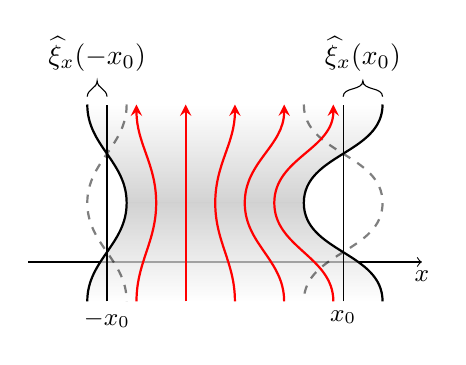
\begin{tikzpicture}
				\draw [->] (1,0) -- (6,0);
				
				\shade[bottom color=lightgray,top color=white, opacity=0.7] (1.75,2) to [out=-90,in=90] (2.25,0.75) to (4.5,0.75) to [out=90,in=-90] (5.5,2) to (1.75,2);
				
				\shade[bottom color=white,top color=lightgray, opacity=0.7] (2.25,0.75) to (4.5,0.75) to [out=-90,in=90] (5.5,-0.5) to (1.75,-0.5) to [out=90,in=-90] (2.25,0.75);
				
				\draw [thick] (1.75,2) to [out=-90,in=90] (2.25,0.75) to [out=-90,in=90] (1.75,-0.5);
				\draw [thick, dashed, opacity=0.5] (4.5,2) to [out=-90,in=90] (5.5,0.75) to [out=-90,in=90] (4.5,-0.5);
				
				\draw [thick, red, -stealth] (2.375,-0.5) to [out=90,in=-90] (2.625, 0.75) to [out=90,in=-90] (2.375,2);
				\draw [thick, red, -stealth] (3,-0.5) to [out=90,in=-90] (3, 0.75) to [out=90,in=-90] (3,2);
				\draw [thick, red, -stealth] (3.625,-0.5) to [out=90,in=-90] (3.375, 0.75) to [out=90,in=-90] (3.625,2);
				\draw [thick, red, -stealth] (4.25,-0.5) to [out=90,in=-90] (3.75, 0.75) to [out=90,in=-90] (4.25,2);
				\draw [thick, red, -stealth] (4.875,-0.5) to [out=90,in=-90] (4.125, 0.75) to [out=90,in=-90] (4.875,2);
				
				\draw [thick, dashed, opacity=0.5] (2.25,2) to [out=-90,in=90] (1.75,0.75) to [out=-90,in=90] (2.25,-0.5);
				\draw [thick] (5.5,2) to [out=-90,in=90] (4.5,0.75) to [out=-90,in=90] (5.5,-0.5);
				
				% % % % % % % % % % % % % % % % % % % % % % % % % %
				
				%\draw [->] (0,0) -- (0,2);
				
				%\node at (1,1) {$\rho_1$};
				%\node at (6,1) {$\rho_2$};
				%\node [right] at (2.95,1.3) {$\rho_0$};
				
				\draw [-] (1.75, 2.1) to [out=90, in=-90] (1.875, 2.3) to [out=-90, in=90] (2, 2.1);
				\draw [-] (5, 2.1) to [out=90, in=-90] (5.25, 2.3) to [out=-90, in=90] (5.5, 2.1);
				
				\node [above] at (1.875,2.3) {$\widehat{\xi}_x(-x_0)$};
				\node [above] at (5.25, 2.3) {$\widehat{\xi}_x(x_0)$};
				
				\small
				\node [below] at (2,-0.5) {$-x_0$};
				\node [below] at (5,-0.5) {$x_0$};
				
				%\node [left] at (0,2) {$z$};
				\node [below] at (6,0) {$x$};
				\draw [-] (2,-0.5) -- (2,2);
				\draw [-] (5,-0.5) -- (5,2);
				\end{tikzpicture} 
			}\label{fig: RA saus}}
		
		
		\subfloat[]{\scalebox{0.9}{
				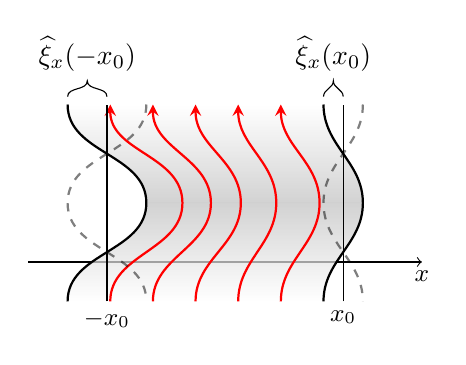
\begin{tikzpicture}
				\draw [->] (1,0) -- (6,0);
				
				\shade[bottom color=lightgray,top color=white, opacity=0.7] (1.5,2) to [out=-90,in=90] (2.5,0.75) to (5.25,0.75) to [out=90,in=-90] (4.75,2) to (1.5,2);
				
				\shade[bottom color=white,top color=lightgray, opacity=0.7] (2.5,0.75) to (5.25,0.75) to [out=-90,in=90] (4.75,-0.5) to (1.5,-0.5) to [out=90,in=-90] (2.5,0.75);
				
				\draw [thick] (1.5,2) to [out=-90,in=90] (2.5,0.75) to [out=-90,in=90] (1.5,-0.5);
				\draw [thick] (4.75,2) to [out=-90,in=90] (5.25,0.75) to [out=-90,in=90] (4.75,-0.5);
				
				%\draw [thick, red, -stealth] (2.0417,-0.5) to [out=90,in=-90] (2.9583, 0.75) to [out=90,in=-90] (2.0417,2);
				%\draw [thick, red, -stealth] (2.5833,-0.5) to [out=90,in=-90] (3.4167, 0.75) to [out=90,in=-90] (2.5833,2);
				%\draw [thick, red, -stealth] (3.125,-0.5) to [out=90,in=-90] (3.875, 0.75) to [out=90,in=-90] (3.125,2);
				%\draw [thick, red, -stealth] (3.6667,-0.5) to [out=90,in=-90] (4.3333, 0.75) to [out=90,in=-90] (3.6667,2);
				%\draw [thick, red, -stealth] (4.2083,-0.5) to [out=90,in=-90] (4.7917, 0.75) to [out=90,in=-90] (4.2083,2);
				
				\draw [thick, red, -stealth] (2.0417,-0.5) to [out=90,in=-90] (2.9583, 0.75) to [out=90,in=-90] (2.0417,2);
				\draw [thick, red, -stealth] (2.5833,-0.5) to [out=90,in=-90] (3.32, 0.75) to [out=90,in=-90] (2.5833,2);
				\draw [thick, red, -stealth] (3.125,-0.5) to [out=90,in=-90] (3.7, 0.75) to [out=90,in=-90] (3.125,2);
				\draw [thick, red, -stealth] (3.6667,-0.5) to [out=90,in=-90] (4.15, 0.75) to [out=90,in=-90] (3.6667,2);
				\draw [thick, red, -stealth] (4.2083,-0.5) to [out=90,in=-90] (4.7, 0.75) to [out=90,in=-90] (4.2083,2);
				
				\draw [thick, dashed, opacity=0.5] (2.5,2) to [out=-90,in=90] (1.5,0.75) to [out=-90,in=90] (2.5,-0.5);
				\draw [thick, dashed, opacity=0.5] (5.25,2) to [out=-90,in=90] (4.75,0.75) to [out=-90,in=90] (5.25,-0.5);
				
				% % % % % % % % % % % % % % % % % % % % % % % % % %
				
				\draw [-] (1.5, 2.1) to [out=90, in=-90] (1.75, 2.3) to [out=-90, in=90] (2., 2.1);
				\draw [-] (4.75, 2.1) to [out=90, in=-90] (4.875, 2.3) to [out=-90, in=90] (5., 2.1);
				
				\node [above] at (1.75,2.3) {$\widehat{\xi}_x(-x_0)$};
				\node [above] at (4.875, 2.3) {$\widehat{\xi}_x(x_0)$};
				
				\small
				\node [below] at (2,-0.5) {$-x_0$};
				\node [below] at (5,-0.5) {$x_0$};
				
				%\node [left] at (0,2) {$z$};
				\node [below] at (6,0) {$x$};
				\draw [-] (2,-0.5) -- (2,2);
				\draw [-] (5,-0.5) -- (5,2);
				\end{tikzpicture} 
			}\label{fig: RA kink}}}
	\caption{Illustration of the difference in amplitude of oscillation on each boundary of the slab for~\protect\subref{fig: RA saus}~quasi-sausage and~\protect\subref{fig: RA kink}~quasi-kink modes.}
	\label{fig: RA}
\end{figure}

We now define the \emph{amplitude ratio}, $R_\textrm{A} := \hat{\xi}_x(x_0) / \hat{\xi}_x(-x_0)$, as the ratio of the amplitude of oscillation of the left interface ($x = x_0$) to that of the right interface ($x = -x_0$) (see Figure~\ref{fig: RA}). Given that ${\hat{\xi}_x(x) = i\hat{v}_x(x) / \omega}$, we also have $R_\textrm{A} = \hat{v}_x(x_0) / \hat{v}_x(-x_0)$. Firstly, using Equations~\eqref{v-x_01 C} and~\eqref{vx_02 C}, the amplitude ratio for quasi-sausage modes is
\begin{align}
R_A &= -\frac{\Lambda_0 + \Lambda_1\frac{1}{\tau_0}}{\Lambda_0 + \Lambda_2\frac{1}{\tau_0}} \notag \\
&= -\frac{\rho_1m_2}{\rho_2m_1}\left[\frac{(k^2v_\textrm{A}^2 - \omega^2)m_1\frac{\rho_0}{\rho_1} - \omega^2m_0\coth{m_0x_0}}{(k^2v_\textrm{A}^2 - \omega^2)m_2\frac{\rho_0}{\rho_2} - \omega^2m_0\coth{m_0x_0}}\right]. \label{cross-slab ratio saus}
\end{align}
Using Equations~\eqref{v-x_01 B} and~\eqref{vx_02 B}, the corresponding expression for quasi-kink modes can be obtained, namely
\begin{align}
R_\textrm{A} &= \frac{\Lambda_0 + \Lambda_1\tau_0}{\Lambda_0 + \Lambda_2\tau_0} \notag \\
&= \frac{\rho_1m_2}{\rho_2m_1}\left[\frac{(k^2v_\textrm{A}^2 - \omega^2)m_1\frac{\rho_0}{\rho_1} - \omega^2m_0\tanh{m_0x_0}}{(k^2v_\textrm{A}^2 - \omega^2)m_2\frac{\rho_0}{\rho_2} - \omega^2m_0\tanh{m_0x_0}}\right]. \label{cross-slab ratio kink}
\end{align}
As expected, Equations~\eqref{cross-slab ratio saus} and~\eqref{cross-slab ratio kink} reduce to $R_\textrm{A} = -1$ and $R_\textrm{A} = 1$ for sausage and kink modes, respectively, when the slab is symmetric.

To obtain an approximation for the Alfv\'{e}n speed analytically, an approximation such as these must be applied. The following subsections give the analytical inversion for the Alfv\'{e}n speed, $v_\textrm{A}$, of equations~\eqref{cross-slab ratio saus} and~\eqref{cross-slab ratio kink} under the thin slab, wide slab, incompressible plasma, and low-beta approximations. A numerical inversion procedure that requires no further approximation is discussed in Section~\ref{sec: numerical inversion}. Note that we restrict the parameter inversions to surface modes only, thereby omitting body modes, because the eigenfrequencies and eigenfunctions of body modes are not significantly effected by asymmetry in the external plasma (see Section~\ref{sec: EVP non-mag}) so they are not useful for parameter inversion.


\subsection{Thin slab approximation} \label{sec: AR thin slab}
For surface modes in the thin slab approximation, $kx_0 \ll 1$, \cite{rob81b} showed that $m_0x_0 \ll 1$. Therefore, to quadratic order, $\tanh{m_0x_0} \approx m_0x_0$, and the amplitude ratio for a quasi-sausage surface mode in a thin slab reduces to
\begin{equation}
R_\textrm{A} = -\frac{\rho_1m_2}{\rho_2m_1}\left[\frac{(k^2v_\textrm{A}^2 - \omega^2)m_1x_0\frac{\rho_0}{\rho_1} - \omega^2}{(k^2v_\textrm{A}^2 - \omega^2)m_2x_0\frac{\rho_0}{\rho_2} - \omega^2}\right], 
\end{equation}
which can be rearranged to give the analytical expression
\begin{equation}
v_\textrm{A}^2 = \frac{\omega^2}{k^2} \left[1 + \frac{1}{x_0} \left(\frac{R_\textrm{A}\frac{\rho_2}{\rho_0m_2} + \frac{\rho_1}{\rho_0m_1}}{R_\textrm{A} + 1}\right)\right].
\end{equation}
The amplitude ratio for a thin slab quasi-kink surface mode reduces to
\begin{equation}
R_\textrm{A} = \frac{\rho_1m_2}{\rho_2m_1} \left[\frac{(k^2v_\textrm{A}^2 - \omega^2)m_1\frac{\rho_0}{\rho_1} - \omega^2m_0^2x_0}{(k^2v_\textrm{A}^2 - \omega^2)m_2\frac{\rho_0}{\rho_2} - \omega^2m_0^2x_0}\right], 
\end{equation}
which can be rearranged to give the analytical expression
\begin{equation}
v_\textrm{A}^2 = \frac{\omega^2}{k^2} \left[\frac{c_0^2}{c_0^2 - \frac{\omega^2}{k^2}} + k^2x_0\left(\frac{R_\textrm{A}\frac{\rho_2}{\rho_0m_2} - \frac{\rho_1}{\rho_0m_1}}{R_\textrm{A} - 1}\right)\right]. \label{AR soln kink thin}
\end{equation}

In a thin asymmetric slab, the fast quasi-kink surface mode degenerates due to a cut-off by the external sound speeds becoming distinct \citep{all_etal17} and the slow quasi-kink surface mode has a phase speed that approaches zero in the thin slab limit (see Section~\ref{sec: thin slab}). Therefore, to a good approximation the phase speed is much less than the internal sound speed ($\omega/k \ll c_0$) therefore Equation~\eqref{AR soln kink thin} simplifies to
\begin{equation}
v_\textrm{A}^2 = \frac{\omega^2}{k^2} \left[1 + k^2x_0\left(\frac{R_\textrm{A}\frac{\rho_2}{\rho_0m_2} - \frac{\rho_1}{\rho_0m_1}}{R_\textrm{A} - 1}\right)\right]. \label{AR soln kink thin simplified}
\end{equation}

\subsection{Wide slab approximation} \label{sec: AR wide slab}
The wide slab approximation applies when the slab width is much larger than the wavelength, that is when $kx_0 \gg 1$. In Section~\ref{sec: wide slab}, we showed that the surface mode solutions of a wide asymmetric slab are just the surface modes that propagate along each interface independently.

This is analogous to the mechanical example introduced in Section~\ref{sec: mechanical example}. When the two masses are decoupled by removing the middle spring, equivalently setting $k_0 = 0$, each mass oscillates independently at the natural frequency of that side of the spring-mass system (Figure~\ref{fig: wide slab mechanical analogy}). This decoupling provides a good analogy to the wide slab limit for the magnetic slab. In a wide slab, each interface is effectively \textit{decoupled} and oscillates at its own natural frequency, independent of the other interface. Given that we are considering magneto-acoustic waves, there are two restoring forces, the magnetic tension force and the pressure gradient force, which means that each independent interface has two natural frequencies, corresponding to the fast and slow magneto-acoustic modes. With this understanding of the modes in the wide slab limit, the amplitude ratio, $R_\textrm{A}$, is either $0$ or $\pm\infty$, depending on which interface the wave is propagating and is therefore not useful for magneto-seismology.

\begin{figure}
	\makebox[\textwidth][c]{
		\subfloat[Coupled equilibrium]{\scalebox{0.9}{
				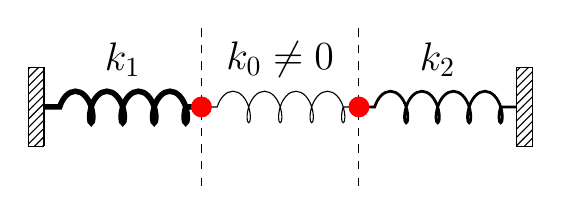
\begin{tikzpicture}
				\filldraw[pattern=north east lines] (0,-0.5) -| (-0.2,0.5) -| (0,-0.5);
				\filldraw[pattern=north east lines] (6,-0.5) -| (6.2,0.5) -| (6,-0.5);
				\draw[Spring, line width=2] (0,0) -- (2,0);
				\draw[Spring, thin] (2,0) -- (4,0);
				\draw[Spring, line width=1] (4,0) -- (6,0);
				
				\draw [dashed] (2,1) -- (2,-1);
				\draw [dashed] (4,1) -- (4,-1);
				
				\draw (2,0) node [fill=red,circle,scale=0.8] {};
				\draw (4,0) node [fill=red,circle,scale=0.8] {};
				
				\Large
				\draw (1,0.6) node [] {$k_1$};
				\draw (3,0.6) node [] {$k_0 \neq 0$};
				\draw (5,0.6) node [] {$k_2$};
				\end{tikzpicture}
		}}
		
		\subfloat[Uncoupled equilibrium]{\scalebox{0.9}{
				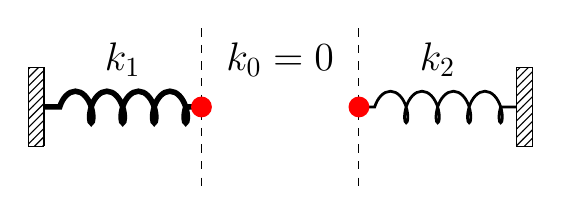
\begin{tikzpicture}
				\filldraw[pattern=north east lines] (0,-0.5) -| (-0.2,0.5) -| (0,-0.5);
				\filldraw[pattern=north east lines] (6,-0.5) -| (6.2,0.5) -| (6,-0.5);
				\draw[Spring, line width=2] (0,0) -- (2,0);
				%\draw[Spring, thin] (2,0) -- (4,0);
				\draw[Spring, line width=1] (4,0) -- (6,0);
				
				\draw [dashed] (2,1) -- (2,-1);
				\draw [dashed] (4,1) -- (4,-1);
				
				\draw (2,0) node [fill=red,circle,scale=0.8] {};
				\draw (4,0) node [fill=red,circle,scale=0.8] {};
				
				\Large
				\draw (1,0.6) node [] {$k_1$};
				\draw (3,0.6) node [] {$k_0 = 0$};
				\draw (5,0.6) node [] {$k_2$};
				\end{tikzpicture}
	}}}
	
	\makebox[\textwidth][c]{
		\subfloat[Uncoupled left oscillation]{\scalebox{0.9}{
				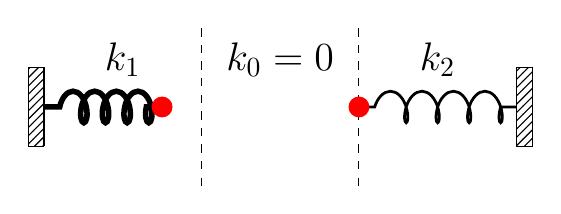
\begin{tikzpicture}
				\filldraw[pattern=north east lines] (0,-0.5) -| (-0.2,0.5) -| (0,-0.5);
				\filldraw[pattern=north east lines] (6,-0.5) -| (6.2,0.5) -| (6,-0.5);
				\draw[Spring, line width=2] (0,0) -- (1.5,0);
				%\draw[Spring, thin] (2,0) -- (4,0);
				\draw[Spring, line width=1] (4,0) -- (6,0);
				
				\draw [dashed] (2,1) -- (2,-1);
				\draw [dashed] (4,1) -- (4,-1);
				
				\draw (1.5,0) node [fill=red,circle,scale=0.8] {};
				\draw (4,0) node [fill=red,circle,scale=0.8] {};
				
				\Large
				\draw (1,0.6) node [] {$k_1$};
				\draw (3,0.6) node [] {$k_0 = 0$};
				\draw (5,0.6) node [] {$k_2$};
				\end{tikzpicture}
		}}
		
		\subfloat[Uncoupled right oscillation]{\scalebox{0.9}{
				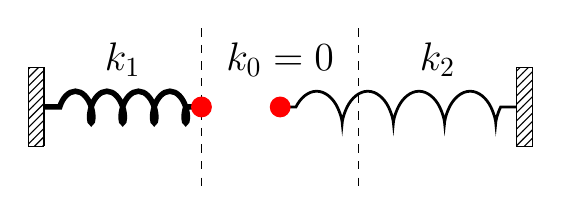
\begin{tikzpicture}
				\filldraw[pattern=north east lines] (0,-0.5) -| (-0.2,0.5) -| (0,-0.5);
				\filldraw[pattern=north east lines] (6,-0.5) -| (6.2,0.5) -| (6,-0.5);
				\draw[Spring, line width=2] (0,0) -- (2,0);
				%\draw[Spring, thin] (2,0) -- (4,0);
				\draw[Spring, line width=1] (3,0) -- (6,0);
				
				\draw [dashed] (2,1) -- (2,-1);
				\draw [dashed] (4,1) -- (4,-1);
				
				\draw (2,0) node [fill=red,circle,scale=0.8] {};
				\draw (3,0) node [fill=red,circle,scale=0.8] {};
				
				\Large
				\draw (1,0.6) node [] {$k_1$};
				\draw (3,0.6) node [] {$k_0 = 0$};
				\draw (5,0.6) node [] {$k_2$};
				\end{tikzpicture}
	}}}
	\caption{Mechanical example showing weak and zero coupling between the masses. This provides an analogy to the wide slab approximation of an asymmetric magnetic slab, in which case the interfaces on each side of the slab oscillate independently.}
	\label{fig: wide slab mechanical analogy}
\end{figure}


\subsection{Incompressible Approximation} \label{sec: AR incomp}

If the plasma is incompressible, the sound speeds become unbounded, so that $m_j \approx k$ for $j = 0, 1, 2$. Under this approximation, the amplitude ratios for quasi-sausage modes (top) and quasi-kink modes (bottom) reduce to
\begin{align}
R_\textrm{A} &= \left(\substack{- \\ +}\right) \frac{\rho_1}{\rho_2} \left[ \frac{(k^2v_\textrm{A}^2 - \omega^2)k\frac{\rho_0}{\rho_1} - \omega^2k \left(\begin{matrix} \coth \\ \tanh \end{matrix}\right)(kx_0)}{(k^2v_\textrm{A}^2-\omega^2)k\frac{\rho_0}{\rho_2}-\omega^2k \left(\begin{matrix} \coth \\ \tanh \end{matrix}\right)(kx_0)} \right].
\end{align}
These equations have solutions for $v_\textrm{A}$ given by
\begin{equation}
v_\textrm{A}^2 = \frac{\omega^2}{k^2} \left[ 1 + \left( \frac{R_\textrm{A} \frac{\rho_2}{\rho_0} \left(\substack{+ \\ -}\right) \frac{\rho_1}{\rho_0}}{R_\textrm{A} \left(\substack{+ \\ -}\right) 1} \right) \left(\begin{matrix} \coth \\ \tanh \end{matrix}\right) (kx_0)\right].
\end{equation}


\subsection{Low-Beta Approximation} \label{sec: AR low-beta}

For a low-beta plasma ($\beta = 2\mu_0p_0/B_0^2 \ll 1$), the magnetic pressure dominates the kinetic plasma pressure and the Alfv\'{e}n speed, $v_\textrm{A}$, dominates the sound speed, $c_0$. Therefore, $m_0^2 \approx k^2 - \omega^2/v_\textrm{A}^2$. For waves with phase speed much less than the Alfv\'{e}n speed, a further approximation of $m_0^2 \approx k^2$ can be made, in which case, the amplitude ratios for quasi-sausage modes (top) and quasi-kink modes (bottom) reduce to
\begin{align}
R_\textrm{A} &= \left(\substack{- \\ +}\right) \frac{\rho_1m_2}{\rho_2m_1} \left[ \frac{(k^2v_\textrm{A}^2 - \omega^2)m_1\frac{\rho_0}{\rho_1} - \omega^2k \left(\begin{matrix} \coth \\ \tanh \end{matrix}\right)(kx_0)}{(k^2v_\textrm{A}^2 - \omega^2)m_2\frac{\rho_0}{\rho_2} - \omega^2k \left(\begin{matrix} \coth \\ \tanh \end{matrix}\right)(kx_0)} \right].
\end{align}
These equations can be solved for $v_\textrm{A}$ to give
\begin{equation}
v_\textrm{A}^2 = \frac{\omega^2}{k^2} \left[1 + k \left( \frac{ \frac{\rho_1}{\rho_0m_1} \left(\substack{+ \\ -}\right) R_\textrm{A}\frac{\rho_2}{\rho_0m_2}}{1 \left(\substack{+ \\ -}\right) R_\textrm{A}} \right) \left(\begin{matrix} \coth \\ \tanh \end{matrix}\right) (kx_0)\right].
\end{equation}
We will return to a discussion of the inversion of the amplitude ratio in Section~\ref{sec: numerical inversion}.


%------------------------------------------------------------------------------
\section{Minimum Perturbation Shift Method}
\label{sec: MPSM}
%------------------------------------------------------------------------------

A second spatial magneto-seismology technique uses the shift in the position of minimum wave power from the centre of the slab due to the asymmetry in the external plasma regions as a diagnostic parameter for estimating the slab Alfv\'{e}n speed.

For a symmetric sausage or kink mode, the position of minimum wave power is the central axis of the slab, at $x = 0$. We define $\Delta_\textrm{min}$ to be the displacement (from the central axis of the waveguide) of the position of minimum wave power inside an asymmetric magnetic slab (Figure~\ref{fig: min pert shift}). For quasi-sausage modes, $\Delta_\textrm{min}$ is the solution to $\widehat{v}_x(x) = 0$ under the constraint $|x| < x_0$, and for quasi-kink modes, $\Delta_\textrm{min}$ is the solution to $\textrm{d}\widehat{v}_x (x) / \textrm{d}x = 0$ under the same constraint $|x| < x_0$. The constraint restricts the solutions to being within the slab. 

\begin{figure}
	\makebox[\textwidth][c]{
		\subfloat[]{\scalebox{0.9}{
				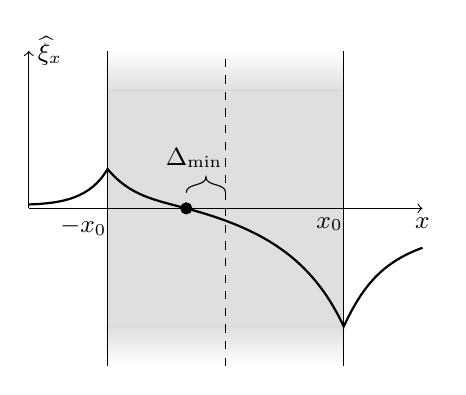
\begin{tikzpicture}
				\path [fill=lightgray, opacity=0.5] (2,-1.5) -- (2,1.5) -- (5,1.5) -- (5,-1.5) -- (2,-1.5);
				
				\shade[bottom color=white,top color=lightgray, opacity=0.5] (2,-2) to (5,-2) to (5,-1.5) to (2,-1.5) to (2,-2);
				
				\shade[top color=white,bottom color=lightgray, opacity=0.5] (2,2) to (5,2) to (5,1.5) to (2,1.5) to (2,2);
				
				\draw [-] (2,-2) -- (2,2);
				\draw [-] (5,-2) -- (5,2);
				
				%\draw [ultra thick, red, -stealth,opacity=0.7] (2.5,-1.5) -- (2.5,2);
				%\draw [ultra thick, red, path fading=south, opacity=0.5] (2.5,-2) -- (2.5,-1.5);
				%\draw [ultra thick, red, -stealth,opacity=0.7] (3,-1.5) -- (3,2);
				%\draw [ultra thick, red, path fading=south,opacity=0.5] (3,-2) -- (3,-1.5);
				%\draw [ultra thick, red, -stealth,opacity=0.7] (3.5,-1.5) -- (3.5,2);
				%\draw [ultra thick, red, path fading=south,opacity=0.5] (3.5,-2) -- (3.5,-1.5);
				%\draw [ultra thick, red, -stealth,opacity=0.7] (4,-1.5) -- (4,2);
				%\draw [ultra thick, red, path fading=south,opacity=0.5] (4,-2) -- (4,-1.5);
				%\draw [ultra thick, red, -stealth,opacity=0.7] (4.5,-1.5) -- (4.5,2);
				%\draw [ultra thick, red, path fading=south,opacity=0.5] (4.5,-2) -- (4.5,-1.5);
				
				%\draw [thick] (0,0.025) to [out=0, in=-178] (1.2, 0.05) to [out=2, in=-120] (2,0.5) to [out=-50, in=165] (3,0) to [out=-15, in=115] (5,-1.5) to [out=65, in=-170] (7,-0.2);
				
				\draw [thick] (1, 0.05) to [out=2, in=-120] (2,0.5) to [out=-50, in=165] (3,0) to [out=-15, in=115] (5,-1.5) to [out=65, in=-160] (6,-0.5);
				
				\draw [->] (1,0) -- (1,2);
				\draw [->] (1,0) -- (6,0);
				
				%\node at (1,1) {$\rho_1$};
				%\node at (6,1) {$\rho_2$};
				%\node [right] at (2.88,1.3) {$\rho_0$};
				
				\small
				\node [below left] at (2.1,0) {$-x_0$};
				\node [below left] at (5.1,0) {$x_0$};
				
				\node [right] at (1,2) {$\widehat{\xi}_x$};
				\node [below] at (6,0) {$x$};
				
				\draw [dashed] (3.5,-2) -- (3.5,2);
				\draw [fill] (3,0) circle [radius=0.07];
				\draw [-] (3, 0.2) to [out=90, in=-90] (3.25, 0.4) to [out=-90, in=90] (3.5, 0.2);
				\node [above] at (3.1, 0.4) {$\Delta_\mathrm{min}$};
				\end{tikzpicture}
			}\label{fig: min pert shift saus}}
		
		
		\subfloat[]{\scalebox{0.9}{
				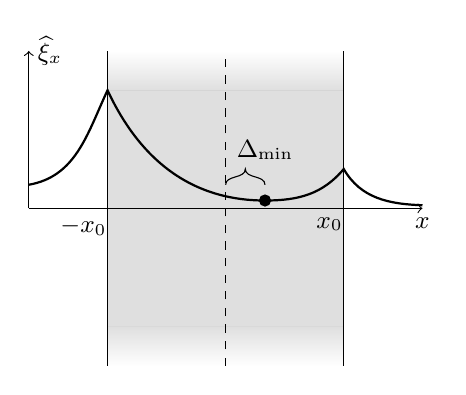
\begin{tikzpicture}
				\path [fill=lightgray, opacity=0.5] (2,-1.5) -- (2,1.5) -- (5,1.5) -- (5,-1.5) -- (2,-1.5);
				
				\shade[bottom color=white,top color=lightgray, opacity=0.5] (2,-2) to (5,-2) to (5,-1.5) to (2,-1.5) to (2,-2);
				
				\shade[top color=white,bottom color=lightgray, opacity=0.5] (2,2) to (5,2) to (5,1.5) to (2,1.5) to (2,2);
				
				\draw [-] (2,-2) -- (2,2);
				\draw [-] (5,-2) -- (5,2);
				
				%\draw [ultra thick, red, -stealth,opacity=0.7] (2.5,-1.5) -- (2.5,2);
				%\draw [ultra thick, red, path fading=south, opacity=0.5] (2.5,-2) -- (2.5,-1.5);
				%\draw [ultra thick, red, -stealth,opacity=0.7] (3,-1.5) -- (3,2);
				%\draw [ultra thick, red, path fading=south,opacity=0.5] (3,-2) -- (3,-1.5);
				%\draw [ultra thick, red, -stealth,opacity=0.7] (3.5,-1.5) -- (3.5,2);
				%\draw [ultra thick, red, path fading=south,opacity=0.5] (3.5,-2) -- (3.5,-1.5);
				%\draw [ultra thick, red, -stealth,opacity=0.7] (4,-1.5) -- (4,2);
				%\draw [ultra thick, red, path fading=south,opacity=0.5] (4,-2) -- (4,-1.5);
				%\draw [ultra thick, red, -stealth,opacity=0.7] (4.5,-1.5) -- (4.5,2);
				%\draw [ultra thick, red, path fading=south,opacity=0.5] (4.5,-2) -- (4.5,-1.5);
				
				%\draw [thick] (0,0.2) to [out=10, in=245] (2, 1.5) to [out=295, in=180] (4,0.1) to [out=0, in=230] (5,0.5) to [out=300, in=178] (6.2,0.04) to [out=358, in=180] (7,0.02);
				
				\draw [thick] (1,0.3) to [out=10, in=245] (2, 1.5) to [out=295, in=180] (4,0.1) to [out=0, in=230] (5,0.5) to [out=300, in=178] (6,0.04);
				
				\draw [->] (1,0) -- (1,2);
				\draw [->] (1,0) -- (6,0);
				%
				%\node at (1,1) {$\rho_1$};
				%\node at (6,1) {$\rho_2$};
				%\node [right] at (2.88,1.3) {$\rho_0$};
				
				\small
				\node [below left] at (2.1,0) {$-x_0$};
				\node [below left] at (5.1,0) {$x_0$};
				
				\node [right] at (1,2) {$\widehat{\xi}_x$};
				\node [below] at (6,0) {$x$};
				
				\draw [dashed] (3.5,-2) -- (3.5,2);
				\draw [fill] (4,0.1) circle [radius=0.07];
				\draw [-] (3.5, 0.3) to [out=90, in=-90] (3.75, 0.5) to [out=-90, in=90] (4, 0.3);
				\node [above] at (4, 0.5) {$\Delta_\mathrm{min}$};
				\end{tikzpicture}
			}\label{fig: min pert shift kink}}}
	
	\caption{Illustration of the minimum perturbation shift, $\Delta_\textrm{min}$, within the slab (shaded) for~\protect\subref{fig: min pert shift saus}~quasi-sausage and~\protect\subref{fig: min pert shift kink}~quasi-kink modes.}
	\label{fig: min pert shift}
\end{figure}

Firstly, for quasi-sausage modes, using the solution for the transversal velocity amplitude given by Equation~\eqref{vsoln} and the expressions for the variables within given by equation~\eqref{constB C}, the minimum perturbation shift can be calculated as follows. The solution for the transversal velocity amplitude within the slab is
\begin{equation}
\widehat{v}_x(x) = B\cosh{m_0x} + C\sinh{m_0x} = 0,
\end{equation}
where $B$ is given by Equation~\eqref{constB C} and $C$ is arbitrary. This equation is solved for $x$ to give
\begin{equation}
x = \frac{1}{m_0} \tanh^{-1}\left(-\frac{B}{C}\right). \label{disp of min power saus}
\end{equation}
Therefore, the minimum perturbation shift for quasi-sausage modes is
\begin{equation}
\Delta_\textrm{min} = \frac{1}{m_0}\tanh^{-1}\left[-\frac{(k^2{v_\textrm{A}}^2 - \omega^2)m_1\frac{\rho_0}{\rho_1} - \omega^2{m_0}\tanh{m_0x_0}}{(k^2{v_\textrm{A}}^2 - \omega^2)m_1\frac{\rho_0}{\rho_1}\tanh{m_0x_0} - \omega^2{m_0}}\right]. \label{shift min saus}
\end{equation}
Similarly, for quasi-kink modes, using Equations~\eqref{vsoln} and~\eqref{constB B}, we calculate the minimum perturbation shift to be
\begin{equation}
\Delta_\textrm{min} = \frac{1}{m_0}\coth^{-1}\left(-\frac{(k^2{v_\textrm{A}}^2 - \omega^2)m_1\frac{\rho_0}{\rho_1} - \omega^2{m_0}\tanh{m_0x_0}}{(k^2{v_\textrm{A}}^2 - \omega^2)m_1\frac{\rho_0}{\rho_1}\tanh{m_0x_0} - \omega^2{m_0}}\right). \label{shift min kink}
\end{equation}
The dependence of the minimum perturbation shifts on the external plasma region with subscript~2 is implicit in the determination of the eigenfrequency $\omega$ when solving the dispersion relation.

The concept of minimum perturbation shift is exclusive to surface modes. The eigenfunctions of surface modes in a magnetic slab are significantly more sensitive to the external plasma parameters than body modes \citep{all_etal17}. This makes intuitive sense given that the energy in a surface mode is localised to the boundaries of the slab whereas the energy in a body mode is largely isolated within the slab. There is a shift in the spatial nodes and anti-nodes in body mode perturbations within a slab due to changing external plasma parameters, however, it is too small to be an effective observational tool.

Akin to the amplitude ratio method for solar magneto-seismology prescribed in Section~\ref{sec: AR}, we can invert Equation~\eqref{shift min saus} or~\eqref{shift min kink} for the the Alfv\'{e}n speed, $v_\textrm{A}$, and hence get an estimate the magnetic field strength of inhomogeneous solar magnetic structures. This can be done either numerically, using an iterative root finding method, or analytically, under an appropriate approximation. In each of the following subsections, we discuss the analytical inversion procedure under the thin slab (Section~\ref{sec: mps thin}), wide slab (Section~\ref{sec: mps wide}), incompressible (Section~\ref{sec: mps incomp}), and low-beta (Section~\ref{sec: mps low-beta}) approximations.


\subsection{Thin slab approximation} \label{sec: mps thin}
Under the thin slab approximation, that is $kx_0 \ll 1$, we have $m_0x_0 \ll 1$ for surface modes (Section~\ref{sec: thin slab}). By definition, $|\Delta_\textrm{min}| < x_0$, therefore, $m_0|\Delta_\textrm{min}| \ll 1$, so that $\tanh{m_0\Delta_\textrm{min}} \approx m_0\Delta_\textrm{min}$. Firstly, for quasi-sausage modes in a thin slab, Equation~\eqref{shift min saus} can be solved for $v_\textrm{A}$ to give
\begin{equation}
v_\textrm{A}^2 = \frac{\omega^2}{k^2} \left[\frac{\rho_1}{\rho_0m_1}(x_0 + \Delta_\textrm{min}) + \frac{1}{1 + (\omega / kc_0)^2} + k^2x_0\Delta_\textrm{min}\right].
\end{equation}
For quasi-kink modes in a thin slab, Equation~\eqref{shift min kink} can be solved for $v_\textrm{A}$ to give
\begin{equation}
v_\textrm{A}^2 = \frac{\omega^2}{k^2}\left[\frac{-b \pm \sqrt{b^2 - 4ac}}{2a}\right],
\end{equation}
where
\begin{align}
a &= m_1\frac{\rho_0}{\rho_1}(k^2c_0^2 - \omega^2)(x_0 + \Delta_\textrm{min}), \\
b &= -m_1\frac{\rho_0}{\rho_1}(2k^2c_0^2 - \omega^2)(x_0 + \Delta_\textrm{min}) - (k^2c_0^2 - \omega^2), \\
c &= c_0^2m_1\frac{\rho_0}{\rho_1}(x_0 + \Delta_\textrm{min}) + c_0^2 + \omega^2x_0\Delta_\textrm{min}.
\end{align}


\subsection{Wide slab approximation} \label{sec: mps wide}
The concept of minimum perturbation shift is ill-defined under the wide slab approximation, that is, when $kx_0 \gg 1$. In this case, each interface oscillates independently at its own eigenfrequency. Therefore the nomenclature of quasi-sausage and quasi-kink mode breaks down. In the wide slab limit, the eigenfunctions have no local minimum in the slab, instead the perturbations are evanescent away from the oscillating interface, therefore there is no local minimum of wave power within the slab.


\subsection{Incompressible approximation} \label{sec: mps incomp}
When the plasma is incompressible, the sound speeds are unbounded, so that $m_j = k$, for $j = 0, 1, 2$. The minimum perturbation shift for a quasi-sausage mode (top) and quasi-kink (bottom) in an incompressible slab is
\begin{equation}
\Delta_\textrm{min} = \frac{1}{k}\left(\begin{matrix} \tanh^{-1} \\ \coth^{-1} \end{matrix}\right)\left(-\frac{(k^2{v_\textrm{A}}^2-\omega^2)\frac{\rho_0}{\rho_1} - \omega^2\tanh{kx_0}}{(k^2{v_\textrm{A}}^2-\omega^2)\frac{\rho_0}{\rho_1}\tanh{kx_0} - \omega^2}\right),
\end{equation}
which can be solved for $v_\textrm{A}$ to give
\begin{equation}
v_\textrm{A}^2 = \frac{\omega^2}{k^2}\left[1 + \frac{\rho_1}{\rho_0}\left(\begin{matrix} \tanh \\ \coth \end{matrix}\right)(k(x_0 + \Delta_\textrm{min}))\right].
\end{equation}


\subsection{Low-beta approximation} \label{sec: mps low-beta}
In a low-beta plasma, the minimum perturbation shift for a quasi-sausage mode (top) and quasi-kink (bottom) is given by
\begin{equation}
\Delta_\textrm{min} = \frac{1}{k}\left(\begin{matrix} \tanh^{-1} \\ \coth^{-1} \end{matrix}\right)\left(-\frac{(k^2{v_\textrm{A}}^2 - \omega^2)m_1\frac{\rho_0}{\rho_1} - \omega^2k\tanh{kx_0}}{(k^2{v_\textrm{A}}^2 - \omega^2)m_1\frac{\rho_0}{\rho_1}\tanh{kx_0} - \omega^2k}\right),
\end{equation}
which can be solved for $v_\textrm{A}$ to give
\begin{equation}
v_\textrm{A}^2 = \frac{\omega^2}{k^2}\left[1 + \frac{k\rho_1}{m_1\rho_0}\left(\begin{matrix} \tanh \\ \coth \end{matrix}\right)(k(x_0 + \Delta_\textrm{min}))\right].
\end{equation}


\begin{sidewaystable}
	\centering
	\begin{tabular}{lccc}
		\toprule
		\smallskip
		Mode & \multicolumn{3}{c}{Approximation of $k^2v_\textrm{A}^2 / \omega^2$ using the amplitude ratio, $R_\textrm{A}$} \\
		& Thin slab & Incompressible & Low-beta \\
		\midrule
		\smallskip
		Quasi-sausage surface & $ 1 + \frac{1}{x_0}\left(\frac{R_\textrm{A}\frac{\rho_2}{\rho_0m_2} + \frac{\rho_1}{\rho_0m_1}}{R_\textrm{A} + 1}\right) $ & $ 1 + \left( \frac{R_\textrm{A} \frac{\rho_2}{\rho_0} + \frac{\rho_1}{\rho_0}}{R_\textrm{A} + 1} \right) \coth{kx_0} $ & $ 1 + k \left( \frac{ R_\textrm{A}\frac{\rho_2}{\rho_0m_2} + \frac{\rho_1}{\rho_0m_1}}{R_\textrm{A} + 1} \right) \coth{kx_0} $ \\
		Quasi-kink surface & $ 1 + k^2x_0\left(\frac{R_\textrm{A}\frac{\rho_2}{\rho_0m_2} - \frac{\rho_1}{\rho_0m_1}}{R_\textrm{A} - 1}\right) $ & $ 1 + \left( \frac{R_\textrm{A} \frac{\rho_2}{\rho_0} - \frac{\rho_1}{\rho_0}}{R_\textrm{A} - 1} \right) \tanh{kx_0} $ & $ 1 + k \left( \frac{ R_\textrm{A}\frac{\rho_2}{\rho_0m_2} - \frac{\rho_1}{\rho_0m_1}}{R_\textrm{A} - 1} \right) \tanh{kx_0} $ \\
		\bottomrule
	\end{tabular}
	\caption{Magneto-seismology inversion using the amplitude ratio, $R_\textrm{A}$, to approximate the Alfv\'{e}n speed, $v_\textrm{A}$.}
	\label{table: amp ratio}

	\bigskip\bigskip\bigskip\bigskip\bigskip

	\begin{tabular}{lccc}
		\toprule
		\smallskip
		Mode & \multicolumn{3}{c}{Approximation of $k^2v_\textrm{A}^2 / \omega^2$ using the minimum perturbation shift, $\Delta_\textrm{min}$} \\
		& Thin slab & Incompressible & Low-beta \\
		\midrule
		\smallskip
		Quasi-sausage surface & $ \frac{\rho_1}{\rho_0m_1}(x_0 + \Delta_\textrm{min}) + \frac{1}{1 + (\omega / kc_0)^2} + k^2x_0\Delta_\textrm{min} $ & $ 1 + \frac{\rho_1}{\rho_0}\tanh{k(x_0 + \Delta_\textrm{min})} $ & $ 1 + \frac{k\rho_1}{m_1\rho_0}\tanh{k(x_0 + \Delta_\textrm{min})} $ \\
		Quasi-kink surface & $\frac{-b \pm \sqrt{b^2 - 4ac}}{2a}$, defined in Section~\ref{sec: mps thin} & $ 1 + \frac{\rho_1}{\rho_0}\coth{k(x_0 + \Delta_\textrm{min})} $ & $ 1 + \frac{k\rho_1}{m_1\rho_0}\coth{k(x_0 + \Delta_\textrm{min})} $ \\
		\bottomrule		
	\end{tabular}
	\caption{Magneto-seismology inversion using the minimum perturbation shift, $\Delta_\textrm{min}$, to approximate the Alfv\'{e}n speed, $v_\textrm{A}$.}
	\label{table: min pert shift}
\end{sidewaystable}


%------------------------------------------------------------------------------
\section{Numerical inversion procedure}
\label{sec: inversion}
%------------------------------------------------------------------------------

We have introduced the amplitude ratio and the minimum perturbation shift which quantify the spatial asymmetry in magnetic slab eigenmodes. These expressions can be applied to determine the Alfv\'{e}n speed, for a given set of observed equilibrium parameters, providing us a novel method to diagnose information about the background plasma, thus advancing the field of spatial magneto-seismology.

A summary of the analytical expressions for estimating the Alfv\'{e}n speed, $v_\textrm{A}$, within an asymmetric magnetic slab is given in Tables~\ref{table: amp ratio} and~\ref{table: min pert shift}, utilising the amplitude ratio method and the minimum perturbation shift method, respectively. With these analytical inversions, theoretical simplicity comes at the cost of having to use an additional approximation.

A second option is to solve the inverse problem numerically. In practice, a numerical procedure could be made relatively simple and computationally inexpensive by making use of a standard root finding method once the observed parameters have been prescribed.


\subsubsection{Estimating a single parameter} \label{sec: single param}

The diagnosis procedure for one background parameter - the Alfv\'{e}n speed, for example - is as follows:
\begin{enumerate}
	\item Observe an oscillating asymmetric MHD waveguide in the solar atmosphere.
	\item Decompose into asymmetric MHD wave modes.
	\item Measure wave parameters: angular frequency and wavelength.
	\item Measure background parameters: waveguide width, density, and temperature (and hence sound speed).
	\item Measure a diagnostic parameter: amplitude ratio or minimum perturbation shift.
	\item Use a root-finding technique to solve the diagnostic equation (Equation~\eqref{cross-slab ratio saus}, \eqref{cross-slab ratio kink}, \eqref{shift min saus}, or~\eqref{shift min kink}, depending on the mode identified and the diagnostic parameter used) for the Alfv\'{e}n speed.
\end{enumerate}
In practice, Step~3 us often extremely difficult. In addition to the Alfv\'{e}n speed, the density across the waveguide is very difficult to measure \citep{war_etal09}. One way around this is to estimate multiple parameters simultaneously, as discussed in Section~\ref{sec: multiple params}.

Figure~\ref{fig: AR MPS} illustrates the dependency of the amplitude ratio and minimum perturbation shift on the (non-dimensionalised half) slab width, $kx_0$, and the density ratio, $\rho_1/\rho_0$, of one external plasma density to the slab density, holding the other external density fixed. Varying one density ratio in this way is equivalent to changing the degree of asymmetry of the waveguide. The amplitude ratio is positive (negative) for quasi-kink (quasi-sausage) modes, because the oscillations on each boundary are in phase (anti-phase). Figures~\ref{fig: AR slow kink surf} and~\ref{fig: AR slow saus surf} further show that, for a given background parameter regime, the boundary with the highest amplitude is different for quasi-kink and quasi-sausage modes. This is demonstrated by the absolute value of the amplitude ratio being greater than 1 for quasi-sausage modes when it is less than 1 for quasi-kink modes, and \textit{vice versa}. This is in agreement with the properties of the eigenmodes of the analogous spring-mass system introduced by \cite{all_etal17} and discussed in Section~\ref{sec: mechanical analogy}. Figures~\ref{fig: MPS slow kink surf} and~\ref{fig: MPS slow saus surf} demonstrate that the position of minimum perturbation for quasi-kink modes is shifted in the opposite direction to that of quasi-sausage modes.

\begin{figure}
	\centering
	\subfloat[Quasi-kink]{\includegraphics[scale=0.38]{\figdir slow-kink-surf_amp-ratio.pdf}
		\label{fig: AR slow kink surf}}
	\subfloat[Quasi-sausage]{\includegraphics[scale=0.38]{\figdir slow-saus-surf_amp-ratio.pdf}
		\label{fig: AR slow saus surf}}
	\\
	\subfloat[Quasi-kink]{\includegraphics[scale=0.38]{\figdir slow-kink-surf_min-pert-shift.pdf}
		\label{fig: MPS slow kink surf}}
	\subfloat[Quasi-sausage]{\includegraphics[scale=0.38]{\figdir slow-saus-surf_min-pert-shift.pdf}
		\label{fig: MPS slow saus surf}}
	\caption{(\protect\subref*{fig: AR slow kink surf}, \protect\subref*{fig: AR slow saus surf}) The amplitude ratio, $R_\textrm{A}$, and (\protect\subref*{fig: MPS slow kink surf}, \protect\subref*{fig: MPS slow saus surf}) the minimum perturbation shift, $\Delta_\textrm{min}$, as a function of the slab width, non-dimensionalised to $kx_0$, and the density ratio, $\rho_1/\rho_0$, for slow (\protect\subref*{fig: AR slow kink surf}, \protect\subref*{fig: MPS slow kink surf}) quasi-kink and (\protect\subref*{fig: AR slow saus surf}, \protect\subref*{fig: MPS slow saus surf}) quasi-sausage surface modes. The other density ratio is set to $\rho_2/\rho_0 = 2$, the characteristic speed ordering inside the slab is $v_\textrm{A}=1.3c_0$, and the sound speed outside the slab is determined to ensure equilibrium pressure balance.}
	\label{fig: AR MPS}
\end{figure}


\subsubsection{Estimating multiple parameters} \label{sec: multiple params}

It is often the case that not all the non-magnetic parameters characterising a waveguide are well-observable. In particular, the density distribution across the waveguide is, like the Alfv\'{e}n speed, often impossible to determine. Thankfully, a combination of the amplitude ratio method and minimum perturbation shift method can be employed to diagnose multiple unknown background parameters. Using a combination of observables to be able to estimate multiple background parameters has been explored by \cite{arr_etal07,Goo_etal08}.

The motivation for this combined technique is as follows. The dispersion relation, the amplitude ratio method, and minimum perturbation shift method give us a set of three functions where the zeros of each function correspond to solutions of the respective equation. Denoting the wave parameters and background parameters by $p_\mathrm{w}$ and $p_\mathrm{bg}$, respectively, these functions (for a quasi-sausage mode) are
\begin{align}
D(p_\mathrm{w}, p_\mathrm{bg}) &= (\Lambda_0c_0 + \Lambda_2s_0)(\Lambda_0s_0 + \Lambda_1c_0) + (\Lambda_0c_0 + \Lambda_1s_0)(\Lambda_0s_0 + \Lambda_2c_0), \label{disp func} \\
f_{\mathrm{AR}}(R_\mathrm{A}, p_\mathrm{w}, p_\mathrm{bg}) &= R_A + \frac{\rho_1m_2}{\rho_2m_1}\left[\frac{(k^2v_\textrm{A}^2 - \omega^2)m_1\frac{\rho_0}{\rho_1} - \omega^2m_0\coth{m_0x_0}}{(k^2v_\textrm{A}^2 - \omega^2)m_2\frac{\rho_0}{\rho_2} - \omega^2m_0\coth{m_0x_0}}\right], \label{AR func} \\
f_{\mathrm{MPS}}(\Delta_\mathrm{min}, p_\mathrm{w}, p_\mathrm{bg}) &= \Delta_\textrm{min} - \frac{1}{m_0}\tanh^{-1}\left[-\frac{(k^2{v_\textrm{A}}^2 - \omega^2)m_1\frac{\rho_0}{\rho_1} - \omega^2{m_0}\tanh{m_0x_0}}{(k^2{v_\textrm{A}}^2 - \omega^2)m_1\frac{\rho_0}{\rho_1}\tanh{m_0x_0} - \omega^2{m_0}}\right]. \label{MPS func} \\
\end{align}
The zeros of each of these functions correspond to solutions of Equations~\eqref{disp rel}, \eqref{cross-slab ratio saus}, and~\eqref{shift min saus}. The single parameter estimation involves using a single-variable root-finding scheme (such as the secant method) to find the zeros of either $f_\mathrm{AR}$ or $f_\mathrm{MPS}$, depending on whether the diagnostic parameter is the amplitude ratio or the minimum perturbation shift (see Section~\ref{sec: single param}). Alternatively, notice that setting Equations~\eqref{disp func}-\eqref{MPS func} to zero forms a system of three coupled equations. Therefore, given measurements of one or two diagnostic parameters, $R_\mathrm{A}$ or $\Delta_\mathrm{min}$, all but up to three background parameters, $p_\mathrm{bg}$, we can use a multivariate root-finding algorithm to solve up to three of these equations. Effectively, the extra diagnostic parameter and the dispersion relation each reduce the number of degrees of freedom. Thus, we can estimate up to three parameters.

As an example, the procedure to estimate the Alfv\'{e}n speed and both the density ratios is as follows:
\begin{enumerate}
	\item Observe an oscillating asymmetric MHD waveguide in the solar atmosphere.
	\item Decompose into asymmetric MHD wave modes.
	\item Measure wave parameters: angular frequency and wavelength.
	\item Measure background parameters: waveguide width and temperature (and hence sound speed).
	\item Measure diagnostic parameters: amplitude ratio and minimum perturbation shift.
	\item Use a multi-variate root-finding algorithm to find the values of the Alfv\'{e}n speed and the two density ratios for which the functions~\eqref{disp func}-\eqref{MPS func} are zero.
\end{enumerate}

As an example, Figure~\ref{fig: vA approx} shows the inversion curves for a particular parameter regime typical of a slow surface mode. It is plotted by prescribing (as if they were observed quantities) all plasma parameters except the Alfv\'{e}n speed, $v_\textrm{A}$, and one of the density ratios, $\rho_1/\rho_0$, then simultaneously solving the dispersion relation, Equation~\eqref{disp rel}, with the equations for the amplitude ratio, Equation~\eqref{cross-slab ratio saus} or~\eqref{cross-slab ratio kink}, or the minimum perturbation shift, Equation~\eqref{shift min saus} or~\eqref{shift min kink}. The solution curves were calculated numerically using Powell's Method, which is an efficient algorithm for calculating the minimum of a multivariate function when the partial derivatives are not available analytically \citep{pow64}.

\begin{figure}
	\centering
	\subfloat[Amplitude ratio inversion]{\includegraphics[scale=0.42]{\figdir RA_vA_approx_2var.pdf}
		\label{fig: RA vA approx}}
	\subfloat[Minimum perturbation shift inversion]{\includegraphics[scale=0.42]{\figdir DM_vA_approx_2var.pdf}
		\label{fig: DM vA approx}}
	\caption{Using prescribed values for~\protect\subref{fig: RA vA approx}~the amplitude ratio, $R_\textrm{A}$, or~\protect\subref{fig: DM vA approx}~the minimum perturbation shift, $\Delta_\textrm{min}$, a numerical inversion is used to approximate the background equilibrium parameters, in this case the Alfv\'{e}n speed, $v_\textrm{A}$, and one of the density ratios, $\rho_1 / \rho_0$, for slow magneto-acoustic modes. Dashed (solid) lines correspond to the inversion curves for slow quasi-kink (quasi-sausage) surface modes. The dotted lines indicate the inversion for symmetric kink and sausage modes. The light-shaded area indicates the values of the Alfv\'{e}n speed which correspond to body modes, rather than surface modes, so are not important for SMS application. The dark shaded region in Figure~\protect\subref{fig: DM vA approx} illustrates the region outside the slab, outside the bounds of the minimum perturbation shift.}
	\label{fig: vA approx}
\end{figure}

The ability to diagnose multiple parameters simultaneously could in some cases get around the hurdle of uncertain density measurements. However, the cost of this is that by estimating several parameters, we are more likely to encounter multiple roots (Section~\ref{sec: multiple roots}).


\subsubsection{Error analysis}

Every measurement comes with error, and when assessing the efficacy of a new measurement technique, an analysis of the errors must be undertaken. There are two kinds of error in a diagnosis made using the AR and MPS methods: \textit{propagated errors} that are due to errors in them measurement of the input parameters, and \textit{systematic errors} that are due to the asymmetric waveguide model approximating the real structure less than perfectly.

To analyse the propagated error, we determine which input parameters are most uncertain and hence are likely to contribute the most uncertainty to the diagnosed parameters. When density is used as an input parameter, it is often the case that the error in its measurement dominates the errors in all other input parameters. Errors in spatial parameters, such as the waveguide width, and temporal parameters, such as the angular frequency, are generally much smaller. The propagation of the error in the density is reduced by a factor of two by the square root that is introduced when inverting $v_A$ from $k^2v_A^2/\omega^2$ (in a similar way to \citealt{nak_etal01}). That is, a relative error of 10\% in the density leads to a relative error of approximately 5\% in the Alfv\'{e}n speed estimation. Furthermore, with high precision methods using density-sensitive emission lines \citep{you_etal09}, the propagation of density measurement errors can be reduced.

As we have seen in Section~\ref{sec: multiple params}, the density need not be an input parameter if both the amplitude ratio and the minimum perturbation shift are observable. In this case, I expect that the input parameter with the highest uncertainty would be the minimum perturbation shift. This is because .... Nevertheless, in the same way as the error in density, the relative error in the measurement of the minimum perturbation shift reduces by a factor of two when propagated through to the relative uncertainty in the estimated parameters. \textcolor{red}{CHECK THIS! HOW DOES THIS WORK WHEN WE ESTIMATE MULTIPLE PARAMS?}

The systematic error is more difficult to analyse quantitatively. The main sources of systematic error include:
\begin{itemize}
	\item The waveguide is not well modelled as an asymmetric slab.
	\item The wave is significantly non-linear.
	\item The wrong solution is found to the parameter inversion (Section~\ref{sec: multiple roots}).
	\item 
\end{itemize}


\subsubsection{Sensitivity to input parameters}

The amplitude ratio has a strong sensitivity to the changes in the external densities, and therefore the external asymmetry, whereas the minimum perturbation shift has a weaker dependency. Therefore, the amplitude ratio is likely to be a more effective parameter for diagnosing background parameters. Furthermore, observations of the location of the minimum wave power within a solar magnetic slab will be fraught with noise, potentially causing the detection of a false minimum. Noise in amplitude ratio measurements is less likely to introduce large errors because the locations of the slab boundaries are a more obvious features and can be identified by the steep gradients in the wavelength of observed light, for example, and is stable to larger noise signals.

Both the amplitude ratio and minimum perturbation shift are more sensitive to small changes in the background equilibrium parameters, \emph{i.e.} the asymmetry in the background plasma, than the eigenfrequencies are. On a theoretical level, this corroborates with the result that eigenfunctions of linear operators on a Hilbert space are often more sensitive to small perturbations of the operator than their corresponding eigenvalues \citep{kat95}. The amplitude ratio and minimum perturbation shift both depend on the eigenfunctions, $\widehat{v}_x(x)$, and their eigenvalues, $\omega^2$. This means that spatial seismology techniques can be theoretically more effective than temporal techniques for many solar structure. Therefore, we are excited to see a push for increased spatial resolution with next-generational observational instrumentation such as the Daniel K. Inouye Solar Telescope (DKIST). Upon completion, this will equip us to be able to use the magneto-seismology techniques developed here to better understand the diagnostic properties of asymmetric slab-like solar atmospheric structures such as elongated magnetic bright points, prominences, and sunspot light walls.


\subsubsection{Dealing with multiple solutions} \label{sec: multiple roots}

A common pitfall when solving inverse problems is identifying the \textit{wrong} solution\footnote{The \textit{wrong} solutions are not wrong in the sense that they don't mathematically solve the equations, rather they are wrong in the sense that they do not map to reality.}. Even the most simple functions can have a multivalued inverse. For example, the function $f(x) = x^2$ has inverse function $f^{-1}(x) = \sqrt(x)$, which is multivalued, for example, $f^{-1}(1) = 1$ or $-1$. If we were looking specifically for the solution $1$ but found only the solution $-1$, we'd have found the \textit{wrong} solution. The original function does not preserve the complete information of the input, so there is no way of getting the missing information when given only the output.

Solar magneto-seismology techniques can lead to problems of a multivalued inverse. In theory, there can be multiple values of the background parameters that will lead to a given observational signature of MHD waves. Therefore, given only the observational signature, is not always possible to find an unambiguous solution to the inverse problem. Sometimes we cannot be sure that our estimation of the background parameters is the correct one, leading to significant systematic error. This problem is more likely to raise its head when attempting to estimate multiple background parameters, such as described in Section~\ref{sec: multiple params}. This is due to there being more dimensions over which the original function can be non-injective. Non-injectivity of the original function is sufficient to guarantee that its inverse function is multivalued. It is even possible for there to be infinitely many solutions to the seismological inverse problems that are all equally likely.

One way around the problem of the multivalued inverse is to use prior information about the MHD waveguide to inform our choice of the correct solution. This is the domain of Bayesian statistics \citep{arr_etal11,arr_etal18}. Bayesian statistics can provide a mathematically precise formulation of multivalued inverse problems in probabilistic terms. It can be used to determine which seismological solution is \textit{more likely} to be correct. For example, let's say we are solving an inverse problem to estimate the magnetic field strength in a quiescent prominence. If we lived in a world where we knew nothing at all about the conditions in a prominence, we would have no way to preference one solution to the inverse problem over another. However, we do not live in that world. Based on several decades worth of of solar observations from tens of solar observatories, we have prior understanding of the range of parameter values we'd expect to observe. We would be more surprised to find a value of 0.01~Gauss or 1000~Gauss than we would for, say, 10~Gauss. Bayesian statistic formalises this probabilistic reasoning. The posterior distribution gives the \textit{degree of belief} of the parameter of interest.

As well as helping to determine which parameter values are more likely to be correct, Bayesian statistics can be useful for model comparison \citep{arr_etal18}. The idea is that estimates of an unknown background parameter are made using multiple models based on data input into each respective seismological method. This provides well defined degrees of belief in each of the models as representing reality best. This is a promising way to reduce the systematic error in seismological inversions.


%------------------------------------------------------------------------------
\section{Discussion of the application of these techniques}
\label{sec: }
%------------------------------------------------------------------------------


\color{red}
There are a number of ways that the amplitude ratio or minimum perturbation shift can be used for spatial seismology. For a given observed wave event in a slab-like solar atmospheric structure, the most simple procedure is as follows. Take measurements for the wave parameters (period and wavelength), and the background parameters (width of structure, plasma density in each region). Determine the sound speeds by assuming equilibrium pressure balance across the slab boundaries. Take a measurement of either the amplitude ratio or minimum perturbation shift. Then invert the corresponding expression for the spatial wave distribution parameter, Equation~\eqref{cross-slab ratio saus}, \eqref{cross-slab ratio kink}, \eqref{shift min saus}, or~\eqref{shift min kink}, to estimate the Alfv\'{e}n speed.





Large magnetic bright points (MBPs), with characteristic length $L > 500$ km, along inter-granular lanes are often rather elongated \citep{cro_etal10}. The application of SMS techniques to MBPs is limited by the low spatial resolution of current observations. DKIST is going to have a spatial resolution of 19 km for structures on the solar surface \citep{tri_etal15}, sufficient enough to resolve oscillations in MBPs. This unprecedented resolution will hopefully give the sufficient number of pixels (5-10) across an MBP to determine whether their oscillations have maximum power at the boundaries of or within the waveguide, that is, to differentiate between the transverse eigenfunctions of surface and body MHD modes, respectively. This is crucial for the accurate employment of these SMS techniques, and would build upon previous work on mode identification such as the surface modes that were identified in photospheric pores \citep{mor_etal15}.

Quiescent prominences, which are large long-lived magnetic formations of cool dense plasma elevated into the hot and rarefied coronal atmosphere, can be approximated by magnetic slabs and have been regularly observed to guide MHD waves \citep{arr_etal12}. The basic slab model of prominences, as illustrated by \textit{e.g.} \cite{joa_etal92a,joa_etal92b}, is of a symmetric slab, however, a small asymmetry could easily be caused by adjacent inhomogeneities. Even a small asymmetry in density ($|1 - \rho_1/\rho_2| < 0.1$) can cause a significant (factor of 2 or more) asymmetry in the eigenmode (Figure~\ref{fig: AR MPS}), except for in thin slabs. This makes prominences a good candidate for applying the SMS techniques developed here. One issue that one has to bear in mind for the employment of these techniques is that the approximation of simple asymmetric magnetic slab may be insufficient to capture some important aspects of prominence oscillations, in particular, prominences are likely to have a sheared magnetic field and may have significant flows, which are neglected in the asymmetric slab model \citep{van_etal89,zir_etal94,bal05,oli09,arr_etal12}.

Light bridge surges also present a possible application for the SMS techniques developed here. Rooted in sunspot light bridges, these clusters of recurrent chromospheric surges observed as bright structures in \textit{e.g.} IRIS 1330~\AA~line, as observed by \citealt{yan_etal16} are formed by either magnetic reconnection just above the light bridge \citep{tor_etal15,rob_etal16} or by leakage of p-modes from beneath the underlying photosphere \citep{yan_etal15,zha_etal17}. They have been demonstrated to guide MHD waves driven by nearby disturbances \citep{yan_etal16,yan_etal17}. While the asymmetric magnetic slab could be a valid approximation for the actual geometry of light walls, the strong magnetic field in the low solar atmosphere above a sunspot umbra (the plasma each side of the light bridge) may put into question the full validity of the non-magnetic external plasma in the current model. However, what matters is the relative strength of the magnetic force compared to the pressure gradient force, that is, the value of plasma-beta. The value of beta above magnetic pores and sunspots is uncertain, but has been shown to be rather high in some cases \citep{bou17}, and has therefore been used in models of the low atmosphere \citep{mum_etal15}. With improved observations, it may turn out that the plasma surrounding light walls has a low-beta, in which case, we suggest that a future generalisation of the methods described here which involves an asymmetric magnetic plasma outside the slab will be a more appropriate method for the first magneto-seismology diagnosis of sunspot light walls.

Of course, these methods have limits of applicability due to the fact that we have modelled the slab as infinitely long, yet there do not exist any infinitely long waveguides in the solar atmosphere. However, if the length, L, of the cross section of an observed solar waveguide is much greater than its width, $x_0$, say $L/x_0=5-10$, then this model of an infinitely long slab may be a valid approximation. Furthermore, if the wavelength of the observed wave, $\lambda$, is such that $L \gg \lambda \gg x_0$, then the thin slab approximation holds (Sections~\ref{sec: AR thin slab} and~\ref{sec: min pert shift thin}), therefore an analytical diagnosis of the Alfv\'{e}n speed within the waveguide can be made using Table~\ref{table: amp ratio} or~\ref{table: min pert shift}.

This paper introduces two novel SMS methods that, for the first time, explore the asymmetry of solar magnetic waveguides to diagnose background parameters. While the simplicity of the current model of an infinitely long slab in a non-magnetic environment introduces several problems with applicability of the methods, the focus is on the novel concept of waveguide asymmetry. Future advancements of these methods involving more complex equilibrium conditions will be valuable in the coming age of high-resolution solar observations. We propose to determine whether asymmetric magneto-acoustic surface waves can be excited within the characteristic lifetime of an asymmetric waveguide in the solar atmosphere. This task can be investigated analytically (for linear waves with simple initial conditions) and numerically (for non-linear waves with more sophisticated initial conditions). Further, a more realistic system, in particular, an asymmetric magnetic fields in the external plasmas, or an equilibrium shear flow, would allow for better application to the solar waveguides discussed above, at the expense of analytic tractability.

\color{black}

%------------------------------------------------------------------------------
\section{Diagnosing the Alfv\'{e}n speed of chromospheric fibrils}
\label{sec: fibrils}
%------------------------------------------------------------------------------

\subsection{Methodology}


\subsection{Results}


\subsection{Discussion}

\subsubsection{Possible alternative causes of observed asymmetry}
Possibilities: 
\begin{itemize}
	\item Asymmetric ICs
	\item Non-collective oscillations
	\item Observational artefact
	\item Overlying oscillating waveguides due to optically thin atmosphere.
\end{itemize}
Include discussion about how to differentiate between these.




\bibliographystyle{plainnat}
\bibliography{../main/references}  

\end{document}

\documentclass[12pt]{../style-files/ociamthesis}
 
\usepackage{amssymb}
\usepackage{titlesec}
\usepackage{amsmath}
\usepackage{float}
\usepackage{graphicx}
\usepackage{caption}
\usepackage{subfig}
\usepackage{xcolor}
\usepackage[section]{placeins}
\usepackage{mathrsfs}
\usepackage{bm}
\usepackage{stmaryrd}
\usepackage{siunitx}
\usepackage{rotating}
\usepackage[utf8]{inputenc}
\usepackage[round]{natbib}
\usepackage{tikz}
\usetikzlibrary{fadings}
\usetikzlibrary{arrows,shapes, positioning}
\usepackage{booktabs}
\usepackage{multirow}
\usepackage{rotating}
\usepackage{tabularx}
\usepackage{makecell}

%%%%%%%%%%%%%%%%%%%%%%%%%%%%%%%%%%%%%%%%%%%%%%%%%%%%%%%%%%%%%%%%%%%%%%%
% the following is to alter tikz settings to improve springs figure.
\usetikzlibrary{decorations.pathmorphing,calc,patterns}
\makeatletter
\def\pgfdecorationspringstraightlinelength{0.5cm}
\def\pgfdecorationspringnumberofelement{8}
\def\pgfdecorationspringnaturallength{5cm}
\pgfkeys{%
	/pgf/decoration/.cd,
	spring straight line length/.code={%
		\pgfmathsetlengthmacro\pgfdecorationspringstraightlinelength{#1}},
	spring natural length/.code={%
		\pgfmathsetlengthmacro\pgfdecorationspringnaturallength{#1}},
	spring number of element/.store in=\pgfdecorationspringnumberofelement
}

\pgfdeclaredecoration{coil spring}{straight line}{%
	\state{straight line}[%
	persistent precomputation = {%
		% Compute the effective length of the spring (without the length
		% of the two straight lines): \pgfdecorationspringeffectivelength
		\pgfmathsetlengthmacro{\pgfdecorationspringeffectivelength}%
		{\pgfdecoratedpathlength-2*\pgfdecorationspringstraightlinelength}
		% Compute the effective length of one coil pattern:
		% \pgfdecorationspringeffectivelengthofonecoil
		\pgfmathsetlengthmacro{\pgfdecorationspringeffectivelengthofonecoil}%
		{\pgfdecorationspringeffectivelength/\pgfdecorationspringnumberofelement}
	},
	width = \pgfdecorationspringstraightlinelength,
	next state = draw spring]{%
		\pgfpathlineto{%
			\pgfqpoint{%
				\pgfdecorationspringstraightlinelength}{0pt}}
	}
	\state{draw spring}%
	[width=\pgfdecorationspringeffectivelengthofonecoil,
	repeat state=\pgfdecorationspringnumberofelement-1,next state=final]{%
		\pgfpathcurveto
		{\pgfpoint@onspringcoil{0    }{ 0.555}{1}}
		{\pgfpoint@onspringcoil{0.445}{ 1    }{2}}
		{\pgfpoint@onspringcoil{1    }{ 1    }{3}}
		\pgfpathcurveto
		{\pgfpoint@onspringcoil{1.555}{ 1    }{4}}
		{\pgfpoint@onspringcoil{2    }{ 0.555}{5}}
		{\pgfpoint@onspringcoil{2    }{ 0    }{6}}
		\pgfpathcurveto
		{\pgfpoint@onspringcoil{2    }{-0.555}{7}}
		{\pgfpoint@onspringcoil{1.555}{-1    }{8}}
		{\pgfpoint@onspringcoil{1    }{-1    }{9}}
		\pgfpathcurveto
		{\pgfpoint@onspringcoil{0.445}{-1    }{10}}
		{\pgfpoint@onspringcoil{0    }{-0.555}{11}}
		{\pgfpoint@onspringcoil{0    }{ 0    }{12}}
	}
	\state{final}{%
		\pgfpathlineto{\pgfpointdecoratedpathlast}
	}
}

\def\pgfpoint@onspringcoil#1#2#3{%
	\pgf@x=#1\pgfdecorationsegmentamplitude%
	\pgf@x=.5\pgf@x%
	\pgf@y=#2\pgfdecorationsegmentamplitude%
	\pgfmathparse{0.083333333333*\pgfdecorationspringeffectivelengthofonecoil}%
	\pgf@xa=\pgfmathresult pt
	\advance\pgf@x by#3\pgf@xa%
}

\makeatother

\tikzset{%
	Spring/.style = {%
		decoration = {%
			coil spring,
			spring straight line length = 0.2cm,
			% To be added
			spring natural length = #1,
			spring number of element = 4,
			amplitude=2mm},
		decorate,
		very thick},
	Spring/.default = {4cm}}
%
%%%%%%%%%%%%%%%%%%%%%%%%%%%%%%%%%%%%%%%%%%%%%%%%%%%%%%%%%%%%%%%%%%%%%%%%%%%%%%%%

\usepackage{geometry}
 \geometry{
 a4paper,
 left=40mm,
 right=30mm,
 top=30mm,
 bottom=30mm
 }

\definecolor{theblue}{HTML}{0000CD}

% disable this package for printed version
\usepackage[colorlinks=true, linktocpage=true, allcolors=theblue]{hyperref}

\titleformat{\chapter}[display]
  {\bfseries\Large}
  {\filright\MakeUppercase{\chaptertitlename} \Large\thechapter}
  {1ex}
  {}
  [\vspace{1ex} \hrule \vspace{1pt} \hrule]

\newcommand{\adv}{    {\it Adv. Space Res.}} 
\newcommand{\annG}{   {\it Ann. Geophys.}} 
\newcommand{\aap}{    {\it Astron. Astrophys.}}
\newcommand{\aaps}{   {\it Astron. Astrophys. Suppl.}}
\newcommand{\aapr}{   {\it Astron. Astrophys. Rev.}}
\newcommand{\ag}{     {\it Ann. Geophys.}}
\newcommand{\aj}{     {\it Astron. J.}} 
\newcommand{\apj}{    {\it Astrophys. J.}}
\newcommand{\apjl}{   {\it Astrophys. J. Lett.}}
\newcommand{\apss}{   {\it Astrophys. Space Sci.}} 
\newcommand{\cjaa}{   {\it Chin. J. Astron. Astrophys.}} 
\newcommand{\gafd}{   {\it Geophys. Astrophys. Fluid Dyn.}}
\newcommand{\grl}{    {\it Geophys. Res. Lett.}}
\newcommand{\ijga}{   {\it Int. J. Geomagn. Aeron.}}
\newcommand{\jastp}{  {\it J. Atmos. Solar-Terr. Phys.}} 
\newcommand{\jgr}{    {\it J. Geophys. Res.}}
\newcommand{\mnras}{  {\it Mon. Not. Roy. Astron. Soc.}}
\newcommand{\na}{     {\it New Astronomy}}
\newcommand{\nat}{    {\it Nature}}
\newcommand{\pasp}{   {\it Pub. Astron. Soc. Pac.}}
\newcommand{\pasj}{   {\it Pub. Astron. Soc. Japan}}
\newcommand{\pre}{    {\it Phys. Rev. E}}
\newcommand{\solphys}{{\it Solar Phys.}}
\newcommand{\sovast}{ {\it Soviet  Astron.}} 
\newcommand{\ssr}{    {\it Space Sci. Rev.}}
\newcommand{\caa}{    {\it Chinese Astron. Astrohpys.}} 
\newcommand{\apjs}{   {\it Astrophys. J. Suppl.}}
\newcommand{\lrsp}{{\it Living Rev. Solar Phys.}}

\newcommand{\bv}{\mathbf{v}}
\newcommand{\bB}{\mathbf{B}}

\newcommand{\figdirV}{../main/figures/chpt-5/} % where figures are stored


\begin{document}

\baselineskip=18pt

\setcounter{secnumdepth}{3}
\setcounter{tocdepth}{3}

\setcounter{chapter}{4}


% include tex file for chapter
%------------------------------------------------------------------------------
\chapter{Asymmetric waveguides - solar magneto-seismology}
\label{chap: SMS}
%------------------------------------------------------------------------------

%------------------------------------------------------------------------------
\section{Chapter introduction}
\label{sec: SMS intro}
%------------------------------------------------------------------------------


In this chapter, we derive two novel techniques for spatial seismology that use an asymmetric slab waveguide to approximate background parameters. This has applications to solar atmospheric structures that are locally slab-like which have been observed to guide MHD oscillations, such as elongated magnetic bright points \citep{yua_etal14}, prominences \citep{arr_etal12}, and light bridge surges \citep{roy73,shi_etal09} (which have also been named light walls by, \textit{e.g.} \citealp{yan_etal15,yan_etal17,zha_etal17}).

We showed in Chapter~\ref{chap: EVP} that a magnetic slab, with non-magnetic, but asymmetric density and temperatures outside the slab has eigenmodes which can be described as either quasi-sausage or quasi-kink. For quasi-sausage (quasi-kink) modes, the oscillations on each slab interface are in anti-phase (phase). They differ in character from traditional (symmetric) sausage and kink modes by their asymmetry about the centre of the slab due to the amplitude of oscillation on each interface being unequal caused by the asymmetric external environment. This results in quasi-kink modes not necessarily retaining their cross-sectional area and quasi-sausage modes not necessarily having reflection symmetric about the centre line of the slab. The spatial distribution of these waves across the slab, and therefore the extent to which they are modified from the traditional sausage and kink modes, is dependent on the asymmetric background plasma parameters. Consequently, we can use the spatial distribution of these waves to diagnose the waveguide. This is the focus of the present chapter: to derive expressions for proxy parameters that encapsulate this asymmetric spatial distribution and discuss the application to SMS.

Sections~\ref{sec: what is SMS} and~\ref{sec: SMS history} give a definition and brief history of SMS. Sections~\ref{sec: AR} and~\ref{sec: MPS} introduce two new SMS techniques: the Amplitude Ratio Method and the Minimum Perturbation Shift Method. Section~\ref{sec: numerical inversion} discusses in more depth the numerical inversion procedure required to apply these two techniques without having to resort to additional approximations. Section~\ref{sec: SMS discussion} discusses where these techniques can be appropriately applied and Section~\ref{sec: fibrils} records the first use of the Amplitude Ratio Method on solar observations.


\subsection{What is solar magneto-seismology?} \label{sec: what is SMS}

Perpetual bubbling, erupting, and turbulent buffeting of plasma drive ubiquitous magneto-acoustic waves throughout the solar atmosphere. The topology and strength of the magnetic field determines the type and properties of waves present in a given structure. Therefore, by observing these waves and solving an inverse problem, it is possible to make a diagnosis of unknown plasma parameters - a class of techniques known as \textit{solar magneto-seismology} (SMS) \citep{and_etal09,arr12,dem_etal12}. This in turn equips us with more realistic parameters for numerical simulations and give us a better understanding of conditions that lead to, for example, wave energy dissipation, instability, magnetic reconnection, and heating.

SMS techniques can be categorised as either \textit{temporal} or \textit{spatial}. Temporal seismology refers to techniques that estimate a plasma parameter by using the observed frequency, or equivalently the period, of waves. Spatial seismology refers to techniques that estimate a plasma parameter by comparing the observed spatial wave power distribution with the eigenfunctions from a theoretical model. Mathematically, the distinction is that temporal seismology techniques use temporal wave parameters (eigenfrequency) only whereas spatial seismology techniques use spatial or a combination of temporal and spatial wave parameters (eigenfunction).

The flowchart in Figure~\ref{fig: SMS} illustrates the causal chain from identifying wave and equilibrium parameters in observations, combining these with eigenmode analysis from models of the physical system, and using SMS techniques to diagnose previously unknown equilibrium parameters.

\newcommand{\tb}{\textcolor{black}}
\tikzstyle{format} = [draw, rounded corners=.055cm, fill=cyan!20]
\tikzstyle{format2} = [draw, rounded corners=.055cm, fill=red!20]
\begin{figure}
	\begin{tikzpicture}[node distance=1.8cm and 3.3cm, auto, >=latex, align = flush center, ultra thick, on grid=true, font=\small]
	% We need to set at bounding box first. Otherwise the diagram
	% will change position for each frame.
	\path[use as bounding box] (-1.7,-4.1) rectangle (10,2);
	\path node[format] (obs) {
		Observations};
	\path node[below= of obs] (ghost) {};
	\path node[format, below= of ghost] (phys) {
		Physical \\ 
		understanding};
	
	\path node[format2, below right= of obs] (ep) {
		Equilibrium \\ 
		parameters};
	\path (ep) edge[<-] (obs);
	\path node[format, above right= of obs] (wp) {
		Wave \\ 
		parameters}
	edge[<-] (obs);
	
	\path node[format, right= of wp] (tp) {
		Temporal \\ 
		parameters}
	edge[<-] (wp);
	\path node[format, below= of tp] (sp) {
		Spatial \\ 
		parameters}
	edge[<-] (wp)
	edge[<-] (ep);  
	
	\path node[format, right= of phys] (em) {
		Equilibrium \\ 
		models};
	\path (em) edge[<-] (phys);
	
	\path node[format, right= of em] (eig) {
		Eigenmodes}
	edge[<-] (em);
	
	\path node[format, right= of sp] (ts) {
		Temporal \\
		magneto-seismology};
	\path (ts) edge[<-] (tp);
	\node at (6.6,-2) (ghost2) {};
	\draw [->] (ghost2.center) -- (ts);
	\draw (ghost2.center) -- (eig);
	\path node[format, below right= of sp] (ss) {
		Spatial \\
		magneto-seismology};
	\draw [->] (eig) -- (ss);
	\path (ss) edge[<-] (sp);
	
	
	\path (ts) edge[->] (ep);
	\path (ss) edge[->] (ep);
	
	\end{tikzpicture}
	\caption{A flow chart illustrating the causal chain of solar magneto-seismology.}
	\label{fig: SMS}
\end{figure}

Several temporal seismology methods have been employed successfully. \cite{ros70} first suggested that the frequency of oscillations, observed through the fluctuation of synchrotron radiation due to the presence of MHD waves, could be used to diagnose background parameters. Further theoretical development has led to more sophisticated temporal methods including local coronal magnetic field strength estimates using standing kink modes in coronal loops by \cite{nak_etal01}, and using slow sausage and kink modes by \cite{erd_etal08}. The ratio of periods of the fundamental and the first harmonic standing kink mode and its dependence on density stratification has also been well studied \citep{ban_etal07,erd_etal14,yu_etal16}.

Spatial seismology techniques have more recently started demonstrating their efficacy in estimating solar parameters. \cite{uch70} estimated the coronal magnetic structure by comparing Moreton wave observations with the theoretical influence that the coronal magnetic field has on the shape of the Moreton wavefront. More recent eigenfunction methods include utilising the anti-node shift of standing modes in a magnetic flux tube to diagnose its inhomogeneous density stratification \citep{erd_etal07,ver_etal07,erd_etal14}.

In this thesis, we particularly focus on diagnosis of the magnetic field. This is because out of all the solar atmospheric features, the magnetic field is often the most elusive and amongst the most dominant in governing solar atmospheric phenomena. It is insightful to consider SMS techniques are part of a larger umbrella of magnetometry techniques, so that the most appropriate technique can be chosen for a given purpose, and to avoid any implication that the new techniques presented in this thesis are useful in every scenario. This broader class of techniques is outlined in Appendix~\ref{app: magnetometry}.


\subsection{A brief history of solar magneto-seismology} \label{sec: SMS history}

To motivate this chapter's focus on developing new temporal seismology techniques, we list a selection of the major advancements in SMS since its development in Table~\ref{table: SMS history}. There are nine major developments in temporal seismology compared to two major developments in spatial seismology. The dominance of the development of temporal seismology techniques over temporal seismology techniques is striking\footnote{Of course, selection bias could have a role to play here.}. Whilst temporal seismology is growing into a mature field, spatial seismology is in its infancy.

% Define custom callouts to shorten the Author column.
\defcitealias{nak_etal01}{Nakariakov et al.}
\defcitealias{arr_etal11}{Arregui et al.}
\defcitealias{erd_etal08}{Erdelyi et al.}
\begin{table}
	\centering
	\begin{tabularx}{\linewidth}{l l X c}
		\toprule
		Date & Author & Description & Type \\
		\midrule
		1970 & \citeauthor{ros70} & Pulsations in synchrotron radiation caused by MHD waves. & T \\
		1970 & \citeauthor{uch70} & Moreton wavefront morphology used to diagnose coronal magnetic structure. & S \\
		1984 & \citeauthor{rob_etal84} & Introduced the theory of coronal seismology. & T \\
		1995 & \citeauthor{tan95} & Prominence seismology. & T \\
		1999 & \makecell[tl]{\citeauthor{asc_etal99} \\ \citeauthor{nak_etal99}}  & First observations of coronal loop oscillations using TRACE. & N \\
		2001 & \citetalias{nak_etal01} & Period of standing kink mode used to diagnose magnetic field strength in coronal loops. & T \\
		2002 & \citeauthor{goo_etal02} & Damping time scales (assuming exponential damping profile) used to estimate density variation across a coronal loop. & T \\
		2005 & \citeauthor{and_etal05} & Density stratification deduced from the period ratio of the first two standing kink harmonics. & T \\
		2007 & \citeauthor{ver_etal07} & Anti-node shift used to diagnose density stratification along the loop. & S \\
		2008 & \citetalias{erd_etal08} & Seismology of slow standing modes in coronal loops. & T \\
		2011 & \citetalias{arr_etal11} & Probabilistic coronal seismology inversion using Bayesian statistics. & N \\
		2013 & \citeauthor{pas_etal13} & A combination of Gaussian and exponential damping of kink modes used to estimate loop density. & T \\
		2017 & \citeauthor{lon_etal17} & Dynamic coronal seismology, \textit{i.e.} diagnosing the magnetic field strength changing in time and across a large portion of the solar atmosphere. Using the methodology developed by \cite{mor_etal15}. & T \\
		\bottomrule
	\end{tabularx}
	\caption{History of solar magneto-seismology development. The \textit{type} column refers to whether the development is in temporal seismology (T), spatial seismology (S), or neither (N).}
	\label{table: SMS history}
\end{table}

Why has spatial seismology lagged behind? There are several plausible answers to this questions. Both ground-based and space-bourne solar telescopes suffer from limitations in spatial resolution. The most significant increases in spatial resolution come from increasing telescope's aperture size. Space-bourne telescopes are limited in this regard because larger aperture size means a larger spacecraft is required to deliver the telescope into orbit. This comes at significant extra cost. Ground-based telescopes suffer from limitations on their spatial resolution from seeing effects, although this has been partially overcome in the era of adaptive optics. These limitations have allowed faster improvements in temporal resolution compared to spatial resolution, therefore the measurement errors in temporal parameters tend to be lower than those in spatial parameters. This means that temporal seismology inversions tend to have lower errors that propagate through from input errors than spatial seismology inversions.

A second plausible explanation is that the development of spatial seismology techniques tends to require more sophisticated MHD wave modelling than temporal seismology techniques. In general, spatial seismology techniques exploit some observational consequence of a deviation of a waveguide from its most simple counterpart to estimate an unknown parameter. For example, the anti-node shift method uses the shift in position (observational consequence of density non-uniformity) of the anti-nodes of standing modes of coronal loops, due to enhanced density in the loop foot-points (deviation from simple model of a uniform flux tube) to estimate the foot-point density (unknown parameter). An interpretation the techniques we will develop in Sections~\ref{sec: AR} and~\ref{sec: MPS} using this framing is that these techniques use the amplitude ratio or minimum perturbation shift (observational consequences of waveguide asymmetry) which exist due to the asymmetry of the waveguide (deviation from the simple symmetric slab model) which are proxies for the strength of the magnetic field (unknown parameter).


%------------------------------------------------------------------------------
\section{Amplitude Ratio}
\label{sec: AR}
%------------------------------------------------------------------------------

The aim of this section is to derive an expression for the ratio of the oscillation amplitude on each interface of an asymmetric magnetic slab in terms of the wave parameters and plasma parameters of the system, then demonstrate how this parameter can be utilised to diagnose background parameters. We focus on estimating the Alfv\'{e}n speed since it is the the most difficult of all our background parameters to measure using traditional methods. We do this by first deriving expressions for the eigenfunctions\footnote{That is, the distribution of the oscillation amplitude across the waveguide.} of quasi-sausage and quasi-kink modes, using them to derive expressions for the Amplitude Ratio, and then by making suitable approximations, we can solve the inverse problem for the Alfv\'{e}n speed. Numerical inversion procedures for the Amplitude Ratio Method are discussed in Section~\ref{sec: numerical inversion}.

\subsection{Deriving an expression for the Amplitude Ratio} \label{sec: AR derivation}

Consider an asymmetric magnetic slab in a non-magnetic environment, as studied in Section~\ref{sec: EVP non-mag} and by \cite{all_etal17}. In this section, we denote the Alfv\'{e}n speed inside the slab as $v_\textrm{A}$ rather than $v_{A0}$ for brevity because it is the only Alfv\'{e}n speed in the system since we have let the external plasma be non-magnetic.

In Section~\ref{sec: EVP non-mag}, it was shown that trapped magneto-acoustic modes propagating along an asymmetric magnetic slab have velocity perturbation in the $x$-direction given by $v_x(x,y,z,t) = \widehat{v}_x(x)e^{i(kz-\omega t)}$, where $\omega$ and $k$ are the angular frequency and wavenumber, and
\begin{equation}
\hat{v}_x(x)=
\begin{cases}
A(\cosh{m_1x} + \sinh{m_1x}) & \text{if } x < -x_0, \\
B\cosh{m_0x} + C\sinh{m_0x} & \text{if } |x| \leq x_0, \\
D(\cosh{m_2x} - \sinh{m_2x}) & \text{if } x > x_0, \label{vsoln}
\end{cases}
\end{equation}
where
\begin{equation}
m_0^2 = \frac{(k^2v_\textrm{A}^2 - \omega^2)(k^2c_0^2 - \omega^2)}{(c_0^2 + v_\textrm{A}^2)(k^2c_{T0}^2-\omega^2)}, \qquad c_{T0}^2 = \frac{c_0^2v_\textrm{A}^2}{c_0^2 + v_\textrm{A}^2}, \label{m0}
\end{equation}
\begin{equation}
m_j^2 = k^2 - \frac{\omega^2}{c_j^2}, \quad \text{for $j = 1, 2$,} \label{m1,2}
\end{equation}
and $A, B, C$, and $D$ are arbitrary constants (with respect to $x$). Therefore, to derive expressions for the eigenfunctions, we need to determine these constants. They can be determined, to within one degree of freedom, using the boundary conditions of continuity in total pressure and transversal velocity component across the slab boundaries at $x = \pm x_0$. Applying these four boundary conditions retrieves four coupled linear homogeneous algebraic equations in the four unknowns, namely
\begin{equation}
\left(
\begin{matrix}
c_1 - s_1 &-c_0                       &s_0                        &0 \\
0       &c_0                        &s_0                        &s_2 - c_2 \\
\Lambda_1(c_1 - s_1)       &\Lambda_0s_0 &-\Lambda_0c_0  &0 \\
0       &\Lambda_0s_0                          &\Lambda                   _0c_0 &-\Lambda_2(s_2 - c_2)
\end{matrix}
\right)
\left(
\begin{matrix}
A \\
B \\
C \\
D
\end{matrix}
\right)
=
\left(
\begin{matrix}
0 \\
0 \\
0 \\
0
\end{matrix}
\right),
\label{coefmatrix}
\end{equation}
where
\begin{equation}
\Lambda_0 = -\frac{i\rho_0(k^2v_\textrm{A}^2 - \omega^2)}{m_0\omega}, \quad \Lambda_1 = \frac{i\rho_1\omega}{m_1}, \quad \text{and} \quad \Lambda_2 = \frac{i\rho_2\omega}{m_2}, \label{Lambdas}
\end{equation}
and $c_i = \cosh{m_ix_0}$ and $s_i = \sinh{m_ix_i}$, for $i = 0, 1, 2$. Ensuring that this matrix has a vanishing determinant gives us the dispersion relation,
\begin{equation}
(\Lambda_0c_0 + \Lambda_2s_0)(\Lambda_0s_0 + \Lambda_1c_0) + (\Lambda_0c_0 + \Lambda_1s_0)(\Lambda_0s_0 + \Lambda_2c_0) = 0. \label{disp rel}
\end{equation}
By satisfying this relation, we gain one degree of freedom in the system of Equations~\eqref{coefmatrix}, which leaves one of the constants $B$ or $C$ arbitrary. This leads to two types of solution: \textit{quasi-sausage} and \textit{quasi-kink} modes.

Firstly, for quasi-sausage modes, by letting $C$ be arbitrary the other constants $A$, $B$, and $D$ can be determined as
\begin{align}
A =& \frac{1}{c_1 - s_1}(Bc_0 - Cs_0), \label{constA C} \\ 
D =& \frac{1}{c_2 - s_2}(Bc_0 + Cs_0), \label{constD C}
\end{align}
where
\begin{equation}
B = \frac{\Lambda_0c_0 + \Lambda_1s_0}{\Lambda_0s_0 + \Lambda_1c_0}C = -\frac{\Lambda_0c_0 + \Lambda_2s_0}{\Lambda_0s_0 + \Lambda_2c_0}C. \label{constB C}
\end{equation}
The second formulation of $B$ in Equation~\eqref{constB C} is found by utilising the dispersion relation, Equation~\eqref{disp rel}. A substitution of these values, using the first form of $B$ in Equation~\eqref{constB C}, into the velocity solution, Equation~\eqref{vsoln}, evaluated at the slab boundaries, yields
\begin{align}
\hat{v}_x(x_0) =& Bc_0 + Cs_0 = \frac{2\Lambda_1 + \Lambda_0\left(\tau_0 + \frac{1}{\tau_0}\right)}{\Lambda_0 + \Lambda_1\frac{1}{\tau_0}}Cc_0, \label{vx_01 C} \\
\hat{v}_x(-x_0) =& Bc_0 - Cs_0 = \frac{\Lambda_0}{\Lambda_0 + \Lambda_1\frac{1}{\tau_0}}C/s_0, \label{v-x_01 C}
\end{align}
where $\tau_0 = \tanh{m_0x_0}$. Similarly, using the second form of $B$ in Equation~\eqref{constB C} yields
\begin{align}
\hat{v}_x(x_0) =& \frac{-\Lambda_0}{\Lambda_0 + \Lambda_2\frac{1}{\tau_0}}C/s_0, \label{vx_02 C} \\
\hat{v}_x(-x_0) =& \frac{-2\Lambda_2 - \Lambda_0\left(\tau_0 + \frac{1}{\tau_0}\right)}{\Lambda_0 + \Lambda_2\frac{1}{\tau_0}}Cc_0. \label{v-x_02 C}
\end{align}
These forms are equivalent. Notice that the horizontal velocity perturbation amplitude, $\hat{v}_x$, is, more precisely, the \emph{signed} amplitude, where a positive (negative) value indicates perturbation in the positive (negative) $x$-direction. This will be important for the inversion procedure.

Secondly, for quasi-kink modes, by letting $B$ be arbitrary, the other constants $A$, $C$, and $D$ can be determined in terms of $B$ as
\begin{align}
A =& \frac{1}{c_1 - s_1}(Bc_0 - Cs_0), \label{constA B} \\ 
D =& \frac{1}{c_2 - s_2}(Bc_0 + Cs_0), \label{constD B}
\end{align}
where
\begin{equation}
C = \frac{\Lambda_0s_0 + \Lambda_1c_0}{\Lambda_0c_0 + \Lambda_1s_0}B = -\frac{\Lambda_0s_0 + \Lambda_2c_0}{\Lambda_0c_0 + \Lambda_2s_0}B. \label{constB B}
\end{equation}
A substitution of these values, using the first form of $C$ in Equation~\eqref{constB B}, into Equation~\eqref{vsoln}, evaluated at the slab boundaries, yields
\begin{align}
\hat{v}_x(x_0) =& \frac{2\Lambda_1 + \Lambda_0\left(\tau_0 + \frac{1}{\tau_0}\right)}{\Lambda_0 + \Lambda_1\tau_0}Bs_0, \label{vx_01 B} \\
\hat{v}_x(-x_0) =& \frac{\Lambda_0}{\Lambda_0 + \Lambda_1\tau_0}B/c_0. \label{v-x_01 B}
\end{align}
Using the second form of $C$ in Equation~\eqref{constB B} yields
\begin{align}
\hat{v}_x(x_0) =& \frac{\Lambda_0}{\Lambda_0 + \Lambda_2\tau_0}B/c_0, \label{vx_02 B} \\
\hat{v}_x(-x_0) =& \frac{2\Lambda_2 + \Lambda_0\left(\tau_0 + \frac{1}{\tau_0}\right)}{\Lambda_0 + \Lambda_2\tau_0}Bs_0. \label{v-x_02 B}
\end{align}

\begin{figure}
	\makebox[\textwidth][c]{
		\subfloat[]{
				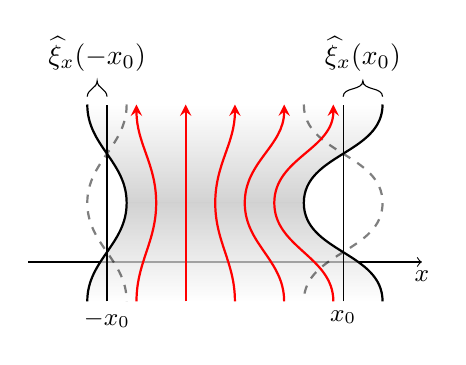
\begin{tikzpicture}
				\draw [->] (1,0) -- (6,0);
				
				\shade[bottom color=lightgray,top color=white, opacity=0.7] (1.75,2) to [out=-90,in=90] (2.25,0.75) to (4.5,0.75) to [out=90,in=-90] (5.5,2) to (1.75,2);
				
				\shade[bottom color=white,top color=lightgray, opacity=0.7] (2.25,0.75) to (4.5,0.75) to [out=-90,in=90] (5.5,-0.5) to (1.75,-0.5) to [out=90,in=-90] (2.25,0.75);
				
				\draw [thick] (1.75,2) to [out=-90,in=90] (2.25,0.75) to [out=-90,in=90] (1.75,-0.5);
				\draw [thick, dashed, opacity=0.5] (4.5,2) to [out=-90,in=90] (5.5,0.75) to [out=-90,in=90] (4.5,-0.5);
				
				\draw [thick, red, -stealth] (2.375,-0.5) to [out=90,in=-90] (2.625, 0.75) to [out=90,in=-90] (2.375,2);
				\draw [thick, red, -stealth] (3,-0.5) to [out=90,in=-90] (3, 0.75) to [out=90,in=-90] (3,2);
				\draw [thick, red, -stealth] (3.625,-0.5) to [out=90,in=-90] (3.375, 0.75) to [out=90,in=-90] (3.625,2);
				\draw [thick, red, -stealth] (4.25,-0.5) to [out=90,in=-90] (3.75, 0.75) to [out=90,in=-90] (4.25,2);
				\draw [thick, red, -stealth] (4.875,-0.5) to [out=90,in=-90] (4.125, 0.75) to [out=90,in=-90] (4.875,2);
				
				\draw [thick, dashed, opacity=0.5] (2.25,2) to [out=-90,in=90] (1.75,0.75) to [out=-90,in=90] (2.25,-0.5);
				\draw [thick] (5.5,2) to [out=-90,in=90] (4.5,0.75) to [out=-90,in=90] (5.5,-0.5);
				
				% % % % % % % % % % % % % % % % % % % % % % % % % %
				
				%\draw [->] (0,0) -- (0,2);
				
				%\node at (1,1) {$\rho_1$};
				%\node at (6,1) {$\rho_2$};
				%\node [right] at (2.95,1.3) {$\rho_0$};
				
				\draw [-] (1.75, 2.1) to [out=90, in=-90] (1.875, 2.3) to [out=-90, in=90] (2, 2.1);
				\draw [-] (5, 2.1) to [out=90, in=-90] (5.25, 2.3) to [out=-90, in=90] (5.5, 2.1);
				
				\node [above] at (1.875,2.3) {$\widehat{\xi}_x(-x_0)$};
				\node [above] at (5.25, 2.3) {$\widehat{\xi}_x(x_0)$};
				
				\small
				\node [below] at (2,-0.5) {$-x_0$};
				\node [below] at (5,-0.5) {$x_0$};
				
				%\node [left] at (0,2) {$z$};
				\node [below] at (6,0) {$x$};
				\draw [-] (2,-0.5) -- (2,2);
				\draw [-] (5,-0.5) -- (5,2);
				\end{tikzpicture} 
			\label{fig: RA saus}}
		
		
		\subfloat[]{
				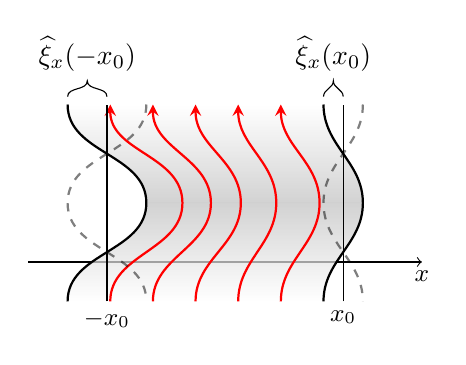
\begin{tikzpicture}
				\draw [->] (1,0) -- (6,0);
				
				\shade[bottom color=lightgray,top color=white, opacity=0.7] (1.5,2) to [out=-90,in=90] (2.5,0.75) to (5.25,0.75) to [out=90,in=-90] (4.75,2) to (1.5,2);
				
				\shade[bottom color=white,top color=lightgray, opacity=0.7] (2.5,0.75) to (5.25,0.75) to [out=-90,in=90] (4.75,-0.5) to (1.5,-0.5) to [out=90,in=-90] (2.5,0.75);
				
				\draw [thick] (1.5,2) to [out=-90,in=90] (2.5,0.75) to [out=-90,in=90] (1.5,-0.5);
				\draw [thick] (4.75,2) to [out=-90,in=90] (5.25,0.75) to [out=-90,in=90] (4.75,-0.5);
				
				%\draw [thick, red, -stealth] (2.0417,-0.5) to [out=90,in=-90] (2.9583, 0.75) to [out=90,in=-90] (2.0417,2);
				%\draw [thick, red, -stealth] (2.5833,-0.5) to [out=90,in=-90] (3.4167, 0.75) to [out=90,in=-90] (2.5833,2);
				%\draw [thick, red, -stealth] (3.125,-0.5) to [out=90,in=-90] (3.875, 0.75) to [out=90,in=-90] (3.125,2);
				%\draw [thick, red, -stealth] (3.6667,-0.5) to [out=90,in=-90] (4.3333, 0.75) to [out=90,in=-90] (3.6667,2);
				%\draw [thick, red, -stealth] (4.2083,-0.5) to [out=90,in=-90] (4.7917, 0.75) to [out=90,in=-90] (4.2083,2);
				
				\draw [thick, red, -stealth] (2.0417,-0.5) to [out=90,in=-90] (2.9583, 0.75) to [out=90,in=-90] (2.0417,2);
				\draw [thick, red, -stealth] (2.5833,-0.5) to [out=90,in=-90] (3.32, 0.75) to [out=90,in=-90] (2.5833,2);
				\draw [thick, red, -stealth] (3.125,-0.5) to [out=90,in=-90] (3.7, 0.75) to [out=90,in=-90] (3.125,2);
				\draw [thick, red, -stealth] (3.6667,-0.5) to [out=90,in=-90] (4.15, 0.75) to [out=90,in=-90] (3.6667,2);
				\draw [thick, red, -stealth] (4.2083,-0.5) to [out=90,in=-90] (4.7, 0.75) to [out=90,in=-90] (4.2083,2);
				
				\draw [thick, dashed, opacity=0.5] (2.5,2) to [out=-90,in=90] (1.5,0.75) to [out=-90,in=90] (2.5,-0.5);
				\draw [thick, dashed, opacity=0.5] (5.25,2) to [out=-90,in=90] (4.75,0.75) to [out=-90,in=90] (5.25,-0.5);
				
				% % % % % % % % % % % % % % % % % % % % % % % % % %
				
				\draw [-] (1.5, 2.1) to [out=90, in=-90] (1.75, 2.3) to [out=-90, in=90] (2., 2.1);
				\draw [-] (4.75, 2.1) to [out=90, in=-90] (4.875, 2.3) to [out=-90, in=90] (5., 2.1);
				
				\node [above] at (1.75,2.3) {$\widehat{\xi}_x(-x_0)$};
				\node [above] at (4.875, 2.3) {$\widehat{\xi}_x(x_0)$};
				
				\small
				\node [below] at (2,-0.5) {$-x_0$};
				\node [below] at (5,-0.5) {$x_0$};
				
				%\node [left] at (0,2) {$z$};
				\node [below] at (6,0) {$x$};
				\draw [-] (2,-0.5) -- (2,2);
				\draw [-] (5,-0.5) -- (5,2);
				\end{tikzpicture} 
			\label{fig: RA kink}}}
	\caption{Illustration of the difference in amplitude of oscillation on each boundary of the slab for~\protect\subref{fig: RA saus}~quasi-sausage and~\protect\subref{fig: RA kink}~quasi-kink modes.}
	\label{fig: RA}
\end{figure}

We now define the \emph{amplitude ratio}, $R_\textrm{A} := \hat{\xi}_x(x_0) / \hat{\xi}_x(-x_0)$, as the ratio of the amplitude of oscillation of the left interface ($x = x_0$) to that of the right interface ($x = -x_0$) (see Figure~\ref{fig: RA}). Given that ${\hat{\xi}_x(x) = i\hat{v}_x(x) / \omega}$, we also have $R_\textrm{A} = \hat{v}_x(x_0) / \hat{v}_x(-x_0)$. Firstly, using Equations~\eqref{v-x_01 C} and~\eqref{vx_02 C}, the amplitude ratio for quasi-sausage modes is
\begin{align}
R_A &= -\frac{\Lambda_0 + \Lambda_1\frac{1}{\tau_0}}{\Lambda_0 + \Lambda_2\frac{1}{\tau_0}} \notag \\
&= -\frac{\rho_1m_2}{\rho_2m_1}\left[\frac{(k^2v_\textrm{A}^2 - \omega^2)m_1\frac{\rho_0}{\rho_1} - \omega^2m_0\coth{m_0x_0}}{(k^2v_\textrm{A}^2 - \omega^2)m_2\frac{\rho_0}{\rho_2} - \omega^2m_0\coth{m_0x_0}}\right]. \label{AR saus}
\end{align}
Using Equations~\eqref{v-x_01 B} and~\eqref{vx_02 B}, the corresponding expression for quasi-kink modes can be obtained, namely
\begin{align}
R_\textrm{A} &= \frac{\Lambda_0 + \Lambda_1\tau_0}{\Lambda_0 + \Lambda_2\tau_0} \notag \\
&= \frac{\rho_1m_2}{\rho_2m_1}\left[\frac{(k^2v_\textrm{A}^2 - \omega^2)m_1\frac{\rho_0}{\rho_1} - \omega^2m_0\tanh{m_0x_0}}{(k^2v_\textrm{A}^2 - \omega^2)m_2\frac{\rho_0}{\rho_2} - \omega^2m_0\tanh{m_0x_0}}\right]. \label{AR kink}
\end{align}
As expected, Equations~\eqref{AR saus} and~\eqref{AR kink} reduce to $R_\textrm{A} = -1$ and $R_\textrm{A} = 1$ for sausage and kink modes, respectively, when the slab is symmetric.

To obtain an approximation for the Alfv\'{e}n speed analytically, an approximation such as these must be applied. The following subsections give the analytical inversion for the Alfv\'{e}n speed, $v_\textrm{A}$, of equations~\eqref{AR saus} and~\eqref{AR kink} under the thin slab, wide slab, incompressible plasma, and low-beta approximations. A numerical inversion procedure that requires no further approximation is discussed in Section~\ref{sec: numerical inversion}. Note that we restrict the parameter inversions to surface modes only, thereby omitting body modes, because the eigenfrequencies and eigenfunctions of body modes are not significantly effected by asymmetry in the external plasma (see Section~\ref{sec: EVP non-mag}) so they are not useful for parameter inversion.


\subsection{Thin slab approximation} \label{sec: AR thin slab}
For surface modes in the thin slab approximation, $kx_0 \ll 1$, \cite{rob81b} showed that $m_0x_0 \ll 1$. Therefore, to quadratic order, $\tanh{m_0x_0} \approx m_0x_0$, and the amplitude ratio for a quasi-sausage surface mode in a thin slab reduces to
\begin{equation}
R_\textrm{A} = -\frac{\rho_1m_2}{\rho_2m_1}\left[\frac{(k^2v_\textrm{A}^2 - \omega^2)m_1x_0\frac{\rho_0}{\rho_1} - \omega^2}{(k^2v_\textrm{A}^2 - \omega^2)m_2x_0\frac{\rho_0}{\rho_2} - \omega^2}\right], 
\end{equation}
which can be rearranged to give the analytical expression
\begin{equation}
v_\textrm{A}^2 = \frac{\omega^2}{k^2} \left[1 + \frac{1}{x_0} \left(\frac{R_\textrm{A}\frac{\rho_2}{\rho_0m_2} + \frac{\rho_1}{\rho_0m_1}}{R_\textrm{A} + 1}\right)\right].
\end{equation}
The amplitude ratio for a thin slab quasi-kink surface mode reduces to
\begin{equation}
R_\textrm{A} = \frac{\rho_1m_2}{\rho_2m_1} \left[\frac{(k^2v_\textrm{A}^2 - \omega^2)m_1\frac{\rho_0}{\rho_1} - \omega^2m_0^2x_0}{(k^2v_\textrm{A}^2 - \omega^2)m_2\frac{\rho_0}{\rho_2} - \omega^2m_0^2x_0}\right], 
\end{equation}
which can be rearranged to give the analytical expression
\begin{equation}
v_\textrm{A}^2 = \frac{\omega^2}{k^2} \left[\frac{c_0^2}{c_0^2 - \frac{\omega^2}{k^2}} + k^2x_0\left(\frac{R_\textrm{A}\frac{\rho_2}{\rho_0m_2} - \frac{\rho_1}{\rho_0m_1}}{R_\textrm{A} - 1}\right)\right]. \label{AR soln kink thin}
\end{equation}

In a thin asymmetric slab, the fast quasi-kink surface mode degenerates due to a cut-off by the external sound speeds becoming distinct \citep{all_etal17} and the slow quasi-kink surface mode has a phase speed that approaches zero in the thin slab limit (see Section~\ref{sec: thin slab}). Therefore, to a good approximation the phase speed is much less than the internal sound speed ($\omega/k \ll c_0$) therefore Equation~\eqref{AR soln kink thin} simplifies to
\begin{equation}
v_\textrm{A}^2 = \frac{\omega^2}{k^2} \left[1 + k^2x_0\left(\frac{R_\textrm{A}\frac{\rho_2}{\rho_0m_2} - \frac{\rho_1}{\rho_0m_1}}{R_\textrm{A} - 1}\right)\right]. \label{AR soln kink thin simplified}
\end{equation}

\subsection{Wide slab approximation} \label{sec: AR wide slab}
The wide slab approximation applies when the slab width is much larger than the wavelength, that is when $kx_0 \gg 1$. In Section~\ref{sec: wide slab}, we showed that the surface mode solutions of a wide asymmetric slab are just the surface modes that propagate along each interface independently.

This is analogous to the mechanical example introduced in Section~\ref{sec: mechanical example}. When the two masses are decoupled by removing the middle spring, equivalently setting $k_0 = 0$, each mass oscillates independently at the natural frequency of that side of the spring-mass system (Figure~\ref{fig: wide slab mechanical analogy}). This decoupling provides a good analogy to the wide slab limit for the magnetic slab. In a wide slab, each interface is effectively \textit{decoupled} and oscillates at its own natural frequency, independent of the other interface. Given that we are considering magneto-acoustic waves, there are two restoring forces, the magnetic tension force and the pressure gradient force, which means that each independent interface has two natural frequencies, corresponding to the fast and slow magneto-acoustic modes. With this understanding of the modes in the wide slab limit, the amplitude ratio, $R_\textrm{A}$, is either $0$ or $\pm\infty$, depending on which interface the wave is propagating and is therefore not useful for magneto-seismology.

\begin{figure}
	\makebox[\textwidth][c]{
		\subfloat[Coupled equilibrium]{\scalebox{0.9}{
				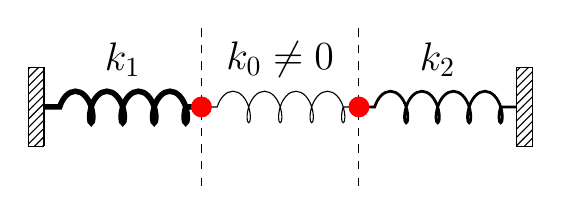
\begin{tikzpicture}
				\filldraw[pattern=north east lines] (0,-0.5) -| (-0.2,0.5) -| (0,-0.5);
				\filldraw[pattern=north east lines] (6,-0.5) -| (6.2,0.5) -| (6,-0.5);
				\draw[Spring, line width=2] (0,0) -- (2,0);
				\draw[Spring, thin] (2,0) -- (4,0);
				\draw[Spring, line width=1] (4,0) -- (6,0);
				
				\draw [dashed] (2,1) -- (2,-1);
				\draw [dashed] (4,1) -- (4,-1);
				
				\draw (2,0) node [fill=red,circle,scale=0.8] {};
				\draw (4,0) node [fill=red,circle,scale=0.8] {};
				
				\Large
				\draw (1,0.6) node [] {$k_1$};
				\draw (3,0.6) node [] {$k_0 \neq 0$};
				\draw (5,0.6) node [] {$k_2$};
				\end{tikzpicture}
		}}
		
		\subfloat[Uncoupled equilibrium]{\scalebox{0.9}{
				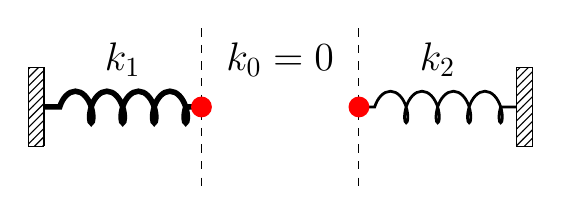
\begin{tikzpicture}
				\filldraw[pattern=north east lines] (0,-0.5) -| (-0.2,0.5) -| (0,-0.5);
				\filldraw[pattern=north east lines] (6,-0.5) -| (6.2,0.5) -| (6,-0.5);
				\draw[Spring, line width=2] (0,0) -- (2,0);
				%\draw[Spring, thin] (2,0) -- (4,0);
				\draw[Spring, line width=1] (4,0) -- (6,0);
				
				\draw [dashed] (2,1) -- (2,-1);
				\draw [dashed] (4,1) -- (4,-1);
				
				\draw (2,0) node [fill=red,circle,scale=0.8] {};
				\draw (4,0) node [fill=red,circle,scale=0.8] {};
				
				\Large
				\draw (1,0.6) node [] {$k_1$};
				\draw (3,0.6) node [] {$k_0 = 0$};
				\draw (5,0.6) node [] {$k_2$};
				\end{tikzpicture}
	}}}
	
	\makebox[\textwidth][c]{
		\subfloat[Uncoupled left oscillation]{\scalebox{0.9}{
				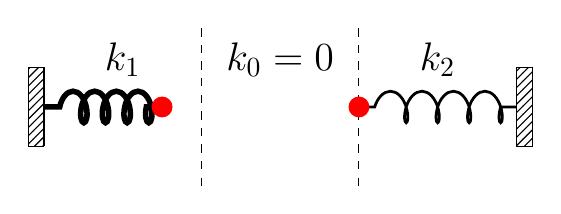
\begin{tikzpicture}
				\filldraw[pattern=north east lines] (0,-0.5) -| (-0.2,0.5) -| (0,-0.5);
				\filldraw[pattern=north east lines] (6,-0.5) -| (6.2,0.5) -| (6,-0.5);
				\draw[Spring, line width=2] (0,0) -- (1.5,0);
				%\draw[Spring, thin] (2,0) -- (4,0);
				\draw[Spring, line width=1] (4,0) -- (6,0);
				
				\draw [dashed] (2,1) -- (2,-1);
				\draw [dashed] (4,1) -- (4,-1);
				
				\draw (1.5,0) node [fill=red,circle,scale=0.8] {};
				\draw (4,0) node [fill=red,circle,scale=0.8] {};
				
				\Large
				\draw (1,0.6) node [] {$k_1$};
				\draw (3,0.6) node [] {$k_0 = 0$};
				\draw (5,0.6) node [] {$k_2$};
				\end{tikzpicture}
		}}
		
		\subfloat[Uncoupled right oscillation]{\scalebox{0.9}{
				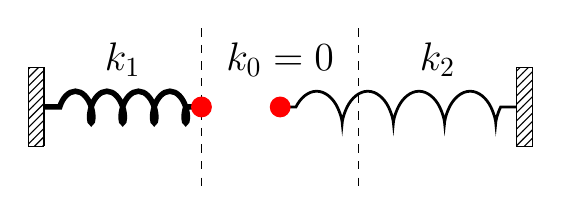
\begin{tikzpicture}
				\filldraw[pattern=north east lines] (0,-0.5) -| (-0.2,0.5) -| (0,-0.5);
				\filldraw[pattern=north east lines] (6,-0.5) -| (6.2,0.5) -| (6,-0.5);
				\draw[Spring, line width=2] (0,0) -- (2,0);
				%\draw[Spring, thin] (2,0) -- (4,0);
				\draw[Spring, line width=1] (3,0) -- (6,0);
				
				\draw [dashed] (2,1) -- (2,-1);
				\draw [dashed] (4,1) -- (4,-1);
				
				\draw (2,0) node [fill=red,circle,scale=0.8] {};
				\draw (3,0) node [fill=red,circle,scale=0.8] {};
				
				\Large
				\draw (1,0.6) node [] {$k_1$};
				\draw (3,0.6) node [] {$k_0 = 0$};
				\draw (5,0.6) node [] {$k_2$};
				\end{tikzpicture}
	}}}
	\caption{Mechanical example showing weak and zero coupling between the masses. This provides an analogy to the wide slab approximation of an asymmetric magnetic slab, in which case the interfaces on each side of the slab oscillate independently.}
	\label{fig: wide slab mechanical analogy}
\end{figure}


\subsection{Incompressible Approximation} \label{sec: AR incomp}

If the plasma is incompressible, the sound speeds become unbounded, so that $m_j \approx k$ for $j = 0, 1, 2$. Under this approximation, the amplitude ratios for quasi-sausage modes (top) and quasi-kink modes (bottom) reduce to
\begin{align}
R_\textrm{A} &= \left(\substack{- \\ +}\right) \frac{\rho_1}{\rho_2} \left[ \frac{(k^2v_\textrm{A}^2 - \omega^2)k\frac{\rho_0}{\rho_1} - \omega^2k \left(\begin{matrix} \coth \\ \tanh \end{matrix}\right)(kx_0)}{(k^2v_\textrm{A}^2-\omega^2)k\frac{\rho_0}{\rho_2}-\omega^2k \left(\begin{matrix} \coth \\ \tanh \end{matrix}\right)(kx_0)} \right].
\end{align}
These equations have solutions for $v_\textrm{A}$ given by
\begin{equation}
v_\textrm{A}^2 = \frac{\omega^2}{k^2} \left[ 1 + \left( \frac{R_\textrm{A} \frac{\rho_2}{\rho_0} \left(\substack{+ \\ -}\right) \frac{\rho_1}{\rho_0}}{R_\textrm{A} \left(\substack{+ \\ -}\right) 1} \right) \left(\begin{matrix} \coth \\ \tanh \end{matrix}\right) (kx_0)\right].
\end{equation}


\subsection{Low-Beta Approximation} \label{sec: AR low-beta}

For a low-beta plasma ($\beta = 2\mu_0p_0/B_0^2 \ll 1$), the magnetic pressure dominates the kinetic plasma pressure and the Alfv\'{e}n speed, $v_\textrm{A}$, dominates the sound speed, $c_0$. Therefore, $m_0^2 \approx k^2 - \omega^2/v_\textrm{A}^2$. For waves with phase speed much less than the Alfv\'{e}n speed, a further approximation of $m_0^2 \approx k^2$ can be made, in which case, the amplitude ratios for quasi-sausage modes (top) and quasi-kink modes (bottom) reduce to
\begin{align}
R_\textrm{A} &= \left(\substack{- \\ +}\right) \frac{\rho_1m_2}{\rho_2m_1} \left[ \frac{(k^2v_\textrm{A}^2 - \omega^2)m_1\frac{\rho_0}{\rho_1} - \omega^2k \left(\begin{matrix} \coth \\ \tanh \end{matrix}\right)(kx_0)}{(k^2v_\textrm{A}^2 - \omega^2)m_2\frac{\rho_0}{\rho_2} - \omega^2k \left(\begin{matrix} \coth \\ \tanh \end{matrix}\right)(kx_0)} \right].
\end{align}
These equations can be solved for $v_\textrm{A}$ to give
\begin{equation}
v_\textrm{A}^2 = \frac{\omega^2}{k^2} \left[1 + k \left( \frac{ \frac{\rho_1}{\rho_0m_1} \left(\substack{+ \\ -}\right) R_\textrm{A}\frac{\rho_2}{\rho_0m_2}}{1 \left(\substack{+ \\ -}\right) R_\textrm{A}} \right) \left(\begin{matrix} \coth \\ \tanh \end{matrix}\right) (kx_0)\right].
\end{equation}
We will return to a discussion of the inversion of the amplitude ratio in Section~\ref{sec: numerical inversion}.


%------------------------------------------------------------------------------
\section{Minimum Perturbation Shift Method}
\label{sec: MPS}
%------------------------------------------------------------------------------

A second spatial magneto-seismology technique uses the shift in the position of minimum wave power from the centre of the slab due to the asymmetry in the external plasma regions as a diagnostic parameter for estimating the slab Alfv\'{e}n speed.

\subsection{Deriving an expression for the minimum perturbation shift} \label{sec: MPS derivation}

For a symmetric sausage or kink mode, the position of minimum wave power is the central axis of the slab, at $x = 0$. We define $\Delta_\textrm{min}$ to be the displacement (from the central axis of the waveguide) of the position of minimum wave power inside an asymmetric magnetic slab (Figure~\ref{fig: min pert shift}). For quasi-sausage modes, $\Delta_\textrm{min}$ is the solution to $\widehat{v}_x(x) = 0$ under the constraint $|x| < x_0$, and for quasi-kink modes, $\Delta_\textrm{min}$ is the solution to $\textrm{d}\widehat{v}_x (x) / \textrm{d}x = 0$ under the same constraint $|x| < x_0$. The constraint restricts the solutions to being within the slab. 

\begin{figure}
	\makebox[\textwidth][c]{
		\subfloat[]{
				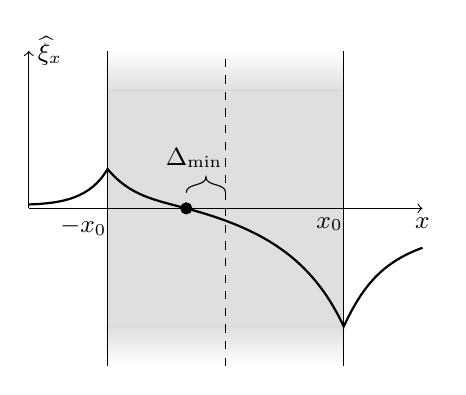
\begin{tikzpicture}
				\path [fill=lightgray, opacity=0.5] (2,-1.5) -- (2,1.5) -- (5,1.5) -- (5,-1.5) -- (2,-1.5);
				
				\shade[bottom color=white,top color=lightgray, opacity=0.5] (2,-2) to (5,-2) to (5,-1.5) to (2,-1.5) to (2,-2);
				
				\shade[top color=white,bottom color=lightgray, opacity=0.5] (2,2) to (5,2) to (5,1.5) to (2,1.5) to (2,2);
				
				\draw [-] (2,-2) -- (2,2);
				\draw [-] (5,-2) -- (5,2);
				
				%\draw [ultra thick, red, -stealth,opacity=0.7] (2.5,-1.5) -- (2.5,2);
				%\draw [ultra thick, red, path fading=south, opacity=0.5] (2.5,-2) -- (2.5,-1.5);
				%\draw [ultra thick, red, -stealth,opacity=0.7] (3,-1.5) -- (3,2);
				%\draw [ultra thick, red, path fading=south,opacity=0.5] (3,-2) -- (3,-1.5);
				%\draw [ultra thick, red, -stealth,opacity=0.7] (3.5,-1.5) -- (3.5,2);
				%\draw [ultra thick, red, path fading=south,opacity=0.5] (3.5,-2) -- (3.5,-1.5);
				%\draw [ultra thick, red, -stealth,opacity=0.7] (4,-1.5) -- (4,2);
				%\draw [ultra thick, red, path fading=south,opacity=0.5] (4,-2) -- (4,-1.5);
				%\draw [ultra thick, red, -stealth,opacity=0.7] (4.5,-1.5) -- (4.5,2);
				%\draw [ultra thick, red, path fading=south,opacity=0.5] (4.5,-2) -- (4.5,-1.5);
				
				%\draw [thick] (0,0.025) to [out=0, in=-178] (1.2, 0.05) to [out=2, in=-120] (2,0.5) to [out=-50, in=165] (3,0) to [out=-15, in=115] (5,-1.5) to [out=65, in=-170] (7,-0.2);
				
				\draw [thick] (1, 0.05) to [out=2, in=-120] (2,0.5) to [out=-50, in=165] (3,0) to [out=-15, in=115] (5,-1.5) to [out=65, in=-160] (6,-0.5);
				
				\draw [->] (1,0) -- (1,2);
				\draw [->] (1,0) -- (6,0);
				
				%\node at (1,1) {$\rho_1$};
				%\node at (6,1) {$\rho_2$};
				%\node [right] at (2.88,1.3) {$\rho_0$};
				
				\small
				\node [below left] at (2.1,0) {$-x_0$};
				\node [below left] at (5.1,0) {$x_0$};
				
				\node [right] at (1,2) {$\widehat{\xi}_x$};
				\node [below] at (6,0) {$x$};
				
				\draw [dashed] (3.5,-2) -- (3.5,2);
				\draw [fill] (3,0) circle [radius=0.07];
				\draw [-] (3, 0.2) to [out=90, in=-90] (3.25, 0.4) to [out=-90, in=90] (3.5, 0.2);
				\node [above] at (3.1, 0.4) {$\Delta_\mathrm{min}$};
				\end{tikzpicture}
			\label{fig: min pert shift saus}}
		
		
		\subfloat[]{
				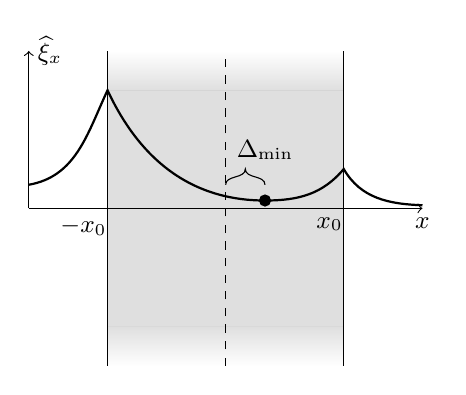
\begin{tikzpicture}
				\path [fill=lightgray, opacity=0.5] (2,-1.5) -- (2,1.5) -- (5,1.5) -- (5,-1.5) -- (2,-1.5);
				
				\shade[bottom color=white,top color=lightgray, opacity=0.5] (2,-2) to (5,-2) to (5,-1.5) to (2,-1.5) to (2,-2);
				
				\shade[top color=white,bottom color=lightgray, opacity=0.5] (2,2) to (5,2) to (5,1.5) to (2,1.5) to (2,2);
				
				\draw [-] (2,-2) -- (2,2);
				\draw [-] (5,-2) -- (5,2);
				
				%\draw [ultra thick, red, -stealth,opacity=0.7] (2.5,-1.5) -- (2.5,2);
				%\draw [ultra thick, red, path fading=south, opacity=0.5] (2.5,-2) -- (2.5,-1.5);
				%\draw [ultra thick, red, -stealth,opacity=0.7] (3,-1.5) -- (3,2);
				%\draw [ultra thick, red, path fading=south,opacity=0.5] (3,-2) -- (3,-1.5);
				%\draw [ultra thick, red, -stealth,opacity=0.7] (3.5,-1.5) -- (3.5,2);
				%\draw [ultra thick, red, path fading=south,opacity=0.5] (3.5,-2) -- (3.5,-1.5);
				%\draw [ultra thick, red, -stealth,opacity=0.7] (4,-1.5) -- (4,2);
				%\draw [ultra thick, red, path fading=south,opacity=0.5] (4,-2) -- (4,-1.5);
				%\draw [ultra thick, red, -stealth,opacity=0.7] (4.5,-1.5) -- (4.5,2);
				%\draw [ultra thick, red, path fading=south,opacity=0.5] (4.5,-2) -- (4.5,-1.5);
				
				%\draw [thick] (0,0.2) to [out=10, in=245] (2, 1.5) to [out=295, in=180] (4,0.1) to [out=0, in=230] (5,0.5) to [out=300, in=178] (6.2,0.04) to [out=358, in=180] (7,0.02);
				
				\draw [thick] (1,0.3) to [out=10, in=245] (2, 1.5) to [out=295, in=180] (4,0.1) to [out=0, in=230] (5,0.5) to [out=300, in=178] (6,0.04);
				
				\draw [->] (1,0) -- (1,2);
				\draw [->] (1,0) -- (6,0);
				%
				%\node at (1,1) {$\rho_1$};
				%\node at (6,1) {$\rho_2$};
				%\node [right] at (2.88,1.3) {$\rho_0$};
				
				\small
				\node [below left] at (2.1,0) {$-x_0$};
				\node [below left] at (5.1,0) {$x_0$};
				
				\node [right] at (1,2) {$\widehat{\xi}_x$};
				\node [below] at (6,0) {$x$};
				
				\draw [dashed] (3.5,-2) -- (3.5,2);
				\draw [fill] (4,0.1) circle [radius=0.07];
				\draw [-] (3.5, 0.3) to [out=90, in=-90] (3.75, 0.5) to [out=-90, in=90] (4, 0.3);
				\node [above] at (4, 0.5) {$\Delta_\mathrm{min}$};
				\end{tikzpicture}
			\label{fig: min pert shift kink}}}
	
	\caption{Illustration of the minimum perturbation shift, $\Delta_\textrm{min}$, within the slab (shaded) for~\protect\subref{fig: min pert shift saus}~quasi-sausage and~\protect\subref{fig: min pert shift kink}~quasi-kink modes.}
	\label{fig: min pert shift}
\end{figure}

Firstly, for quasi-sausage modes, using the solution for the transversal velocity amplitude given by Equation~\eqref{vsoln} and the expressions for the variables within given by equation~\eqref{constB C}, the minimum perturbation shift can be calculated as follows. The solution for the transversal velocity amplitude within the slab is
\begin{equation}
\widehat{v}_x(x) = B\cosh{m_0x} + C\sinh{m_0x} = 0,
\end{equation}
where $B$ is given by Equation~\eqref{constB C} and $C$ is arbitrary. This equation is solved for $x$ to give
\begin{equation}
x = \frac{1}{m_0} \tanh^{-1}\left(-\frac{B}{C}\right). \label{disp of min power saus}
\end{equation}
Therefore, the minimum perturbation shift for quasi-sausage modes is
\begin{equation}
\Delta_\textrm{min} = \frac{1}{m_0}\tanh^{-1}\left[-\frac{(k^2{v_\textrm{A}}^2 - \omega^2)m_1\frac{\rho_0}{\rho_1} - \omega^2{m_0}\tanh{m_0x_0}}{(k^2{v_\textrm{A}}^2 - \omega^2)m_1\frac{\rho_0}{\rho_1}\tanh{m_0x_0} - \omega^2{m_0}}\right]. \label{shift min saus}
\end{equation}
Similarly, for quasi-kink modes, using Equations~\eqref{vsoln} and~\eqref{constB B}, we calculate the minimum perturbation shift to be
\begin{equation}
\Delta_\textrm{min} = \frac{1}{m_0}\coth^{-1}\left(-\frac{(k^2{v_\textrm{A}}^2 - \omega^2)m_1\frac{\rho_0}{\rho_1} - \omega^2{m_0}\tanh{m_0x_0}}{(k^2{v_\textrm{A}}^2 - \omega^2)m_1\frac{\rho_0}{\rho_1}\tanh{m_0x_0} - \omega^2{m_0}}\right). \label{shift min kink}
\end{equation}
The dependence of the minimum perturbation shifts on the external plasma region with subscript~2 is implicit in the determination of the eigenfrequency $\omega$ when solving the dispersion relation.

The concept of minimum perturbation shift is exclusive to surface modes. The eigenfunctions of surface modes in a magnetic slab are significantly more sensitive to the external plasma parameters than body modes \citep{all_etal17}. This makes intuitive sense given that the energy in a surface mode is localised to the boundaries of the slab whereas the energy in a body mode is largely isolated within the slab. There is a shift in the spatial nodes and anti-nodes in body mode perturbations within a slab due to changing external plasma parameters, however, it is too small to be an effective observational tool.

Akin to the amplitude ratio method for solar magneto-seismology prescribed in Section~\ref{sec: AR}, we can invert Equation~\eqref{shift min saus} or~\eqref{shift min kink} for the the Alfv\'{e}n speed, $v_\textrm{A}$, and hence get an estimate the magnetic field strength of inhomogeneous solar magnetic structures. This can be done either numerically, using an iterative root finding method, or analytically, under an appropriate approximation. In each of the following subsections, we discuss the analytical inversion procedure under the thin slab (Section~\ref{sec: mps thin}), wide slab (Section~\ref{sec: mps wide}), incompressible (Section~\ref{sec: mps incomp}), and low-beta (Section~\ref{sec: mps low-beta}) approximations.


\subsection{Thin slab approximation} \label{sec: MPS thin}
Under the thin slab approximation, that is $kx_0 \ll 1$, we have $m_0x_0 \ll 1$ for surface modes (Section~\ref{sec: thin slab}). By definition, $|\Delta_\textrm{min}| < x_0$, therefore, $m_0|\Delta_\textrm{min}| \ll 1$, so that $\tanh{m_0\Delta_\textrm{min}} \approx m_0\Delta_\textrm{min}$. Firstly, for quasi-sausage modes in a thin slab, Equation~\eqref{shift min saus} can be solved for $v_\textrm{A}$ to give
\begin{equation}
v_\textrm{A}^2 = \frac{\omega^2}{k^2} \left[\frac{\rho_1}{\rho_0m_1}(x_0 + \Delta_\textrm{min}) + \frac{1}{1 + (\omega / kc_0)^2} + k^2x_0\Delta_\textrm{min}\right].
\end{equation}
For quasi-kink modes in a thin slab, Equation~\eqref{shift min kink} can be solved for $v_\textrm{A}$ to give
\begin{equation}
v_\textrm{A}^2 = \frac{\omega^2}{k^2}\left[\frac{-b \pm \sqrt{b^2 - 4ac}}{2a}\right],
\end{equation}
where
\begin{align}
a &= m_1\frac{\rho_0}{\rho_1}(k^2c_0^2 - \omega^2)(x_0 + \Delta_\textrm{min}), \\
b &= -m_1\frac{\rho_0}{\rho_1}(2k^2c_0^2 - \omega^2)(x_0 + \Delta_\textrm{min}) - (k^2c_0^2 - \omega^2), \\
c &= c_0^2m_1\frac{\rho_0}{\rho_1}(x_0 + \Delta_\textrm{min}) + c_0^2 + \omega^2x_0\Delta_\textrm{min}.
\end{align}


\subsection{Wide slab approximation} \label{sec: mps wide}
The concept of minimum perturbation shift is ill-defined under the wide slab approximation, that is, when $kx_0 \gg 1$. In this case, each interface oscillates independently at its own eigenfrequency. Therefore the nomenclature of quasi-sausage and quasi-kink mode breaks down. In the wide slab limit, the eigenfunctions have no local minimum in the slab, instead the perturbations are evanescent away from the oscillating interface, therefore there is no local minimum of wave power within the slab.


\subsection{Incompressible approximation} \label{sec: mps incomp}
When the plasma is incompressible, the sound speeds are unbounded, so that $m_j = k$, for $j = 0, 1, 2$. The minimum perturbation shift for a quasi-sausage mode (top) and quasi-kink (bottom) in an incompressible slab is
\begin{equation}
\Delta_\textrm{min} = \frac{1}{k}\left(\begin{matrix} \tanh^{-1} \\ \coth^{-1} \end{matrix}\right)\left(-\frac{(k^2{v_\textrm{A}}^2-\omega^2)\frac{\rho_0}{\rho_1} - \omega^2\tanh{kx_0}}{(k^2{v_\textrm{A}}^2-\omega^2)\frac{\rho_0}{\rho_1}\tanh{kx_0} - \omega^2}\right),
\end{equation}
which can be solved for $v_\textrm{A}$ to give
\begin{equation}
v_\textrm{A}^2 = \frac{\omega^2}{k^2}\left[1 + \frac{\rho_1}{\rho_0}\left(\begin{matrix} \tanh \\ \coth \end{matrix}\right)(k(x_0 + \Delta_\textrm{min}))\right].
\end{equation}


\subsection{Low-beta approximation} \label{sec: mps low-beta}
In a low-beta plasma, the minimum perturbation shift for a quasi-sausage mode (top) and quasi-kink (bottom) is given by
\begin{equation}
\Delta_\textrm{min} = \frac{1}{k}\left(\begin{matrix} \tanh^{-1} \\ \coth^{-1} \end{matrix}\right)\left(-\frac{(k^2{v_\textrm{A}}^2 - \omega^2)m_1\frac{\rho_0}{\rho_1} - \omega^2k\tanh{kx_0}}{(k^2{v_\textrm{A}}^2 - \omega^2)m_1\frac{\rho_0}{\rho_1}\tanh{kx_0} - \omega^2k}\right),
\end{equation}
which can be solved for $v_\textrm{A}$ to give
\begin{equation}
v_\textrm{A}^2 = \frac{\omega^2}{k^2}\left[1 + \frac{k\rho_1}{m_1\rho_0}\left(\begin{matrix} \tanh \\ \coth \end{matrix}\right)(k(x_0 + \Delta_\textrm{min}))\right].
\end{equation}


\begin{sidewaystable}
	\centering
	\begin{tabular}{lccc}
		\toprule
		\smallskip
		Mode & \multicolumn{3}{c}{Approximation of $k^2v_\textrm{A}^2 / \omega^2$ using the amplitude ratio, $R_\textrm{A}$} \\
		& Thin slab & Incompressible & Low-beta \\
		\midrule
		\smallskip
		Quasi-sausage surface & $ 1 + \frac{1}{x_0}\left(\frac{R_\textrm{A}\frac{\rho_2}{\rho_0m_2} + \frac{\rho_1}{\rho_0m_1}}{R_\textrm{A} + 1}\right) $ & $ 1 + \left( \frac{R_\textrm{A} \frac{\rho_2}{\rho_0} + \frac{\rho_1}{\rho_0}}{R_\textrm{A} + 1} \right) \coth{kx_0} $ & $ 1 + k \left( \frac{ R_\textrm{A}\frac{\rho_2}{\rho_0m_2} + \frac{\rho_1}{\rho_0m_1}}{R_\textrm{A} + 1} \right) \coth{kx_0} $ \\
		Quasi-kink surface & $ 1 + k^2x_0\left(\frac{R_\textrm{A}\frac{\rho_2}{\rho_0m_2} - \frac{\rho_1}{\rho_0m_1}}{R_\textrm{A} - 1}\right) $ & $ 1 + \left( \frac{R_\textrm{A} \frac{\rho_2}{\rho_0} - \frac{\rho_1}{\rho_0}}{R_\textrm{A} - 1} \right) \tanh{kx_0} $ & $ 1 + k \left( \frac{ R_\textrm{A}\frac{\rho_2}{\rho_0m_2} - \frac{\rho_1}{\rho_0m_1}}{R_\textrm{A} - 1} \right) \tanh{kx_0} $ \\
		\bottomrule
	\end{tabular}
	\caption{Magneto-seismology inversion using the amplitude ratio, $R_\textrm{A}$, to approximate the Alfv\'{e}n speed, $v_\textrm{A}$.}
	\label{table: amp ratio}

	\bigskip\bigskip\bigskip\bigskip\bigskip

	\begin{tabular}{lccc}
		\toprule
		\smallskip
		Mode & \multicolumn{3}{c}{Approximation of $k^2v_\textrm{A}^2 / \omega^2$ using the minimum perturbation shift, $\Delta_\textrm{min}$} \\
		& Thin slab & Incompressible & Low-beta \\
		\midrule
		\smallskip
		Quasi-sausage surface & $ \frac{\rho_1}{\rho_0m_1}(x_0 + \Delta_\textrm{min}) + \frac{1}{1 + (\omega / kc_0)^2} + k^2x_0\Delta_\textrm{min} $ & $ 1 + \frac{\rho_1}{\rho_0}\tanh{k(x_0 + \Delta_\textrm{min})} $ & $ 1 + \frac{k\rho_1}{m_1\rho_0}\tanh{k(x_0 + \Delta_\textrm{min})} $ \\
		Quasi-kink surface & $\frac{-b \pm \sqrt{b^2 - 4ac}}{2a}$, defined in Section~\ref{sec: mps thin} & $ 1 + \frac{\rho_1}{\rho_0}\coth{k(x_0 + \Delta_\textrm{min})} $ & $ 1 + \frac{k\rho_1}{m_1\rho_0}\coth{k(x_0 + \Delta_\textrm{min})} $ \\
		\bottomrule		
	\end{tabular}
	\caption{Magneto-seismology inversion using the minimum perturbation shift, $\Delta_\textrm{min}$, to approximate the Alfv\'{e}n speed, $v_\textrm{A}$.}
	\label{table: min pert shift}
\end{sidewaystable}


%------------------------------------------------------------------------------
\section{Numerical inversion procedure}
\label{sec: numerical inversion}
%------------------------------------------------------------------------------

We have introduced the amplitude ratio and the minimum perturbation shift which quantify the spatial asymmetry in magnetic slab eigenmodes. These expressions can be applied to determine the Alfv\'{e}n speed, for a given set of observed equilibrium parameters, providing us a novel method to diagnose information about the background plasma, thus advancing the field of spatial magneto-seismology.

A summary of the analytical expressions for estimating the Alfv\'{e}n speed, $v_\textrm{A}$, within an asymmetric magnetic slab is given in Tables~\ref{table: amp ratio} and~\ref{table: min pert shift}, utilising the amplitude ratio method and the minimum perturbation shift method, respectively. With these analytical inversions, theoretical simplicity comes at the cost of having to use an additional approximation.

A second option is to solve the inverse problem numerically. In practice, a numerical procedure could be made relatively simple and computationally inexpensive by making use of a standard root finding method once the observed parameters have been prescribed.


\subsubsection{Estimating a single parameter} \label{sec: single param}

The diagnosis procedure for one background parameter - the Alfv\'{e}n speed, for example - is as follows:
\begin{enumerate}
	\item Observe an oscillating asymmetric MHD waveguide in the solar atmosphere.
	\item Decompose into asymmetric MHD wave modes.
	\item Measure wave parameters: angular frequency and wavelength.
	\item Measure background parameters: waveguide width, density, and temperature (and hence sound speed).
	\item Measure a diagnostic parameter: amplitude ratio or minimum perturbation shift.
	\item Use a root-finding technique to solve the diagnostic equation (Equation~\eqref{AR saus}, \eqref{AR kink}, \eqref{shift min saus}, or~\eqref{shift min kink}, depending on the mode identified and the diagnostic parameter used) for the Alfv\'{e}n speed.
\end{enumerate}
In practice, Step~3 us often extremely difficult. In addition to the Alfv\'{e}n speed, the density across the waveguide is very difficult to measure \citep{war_etal09}. One way around this is to estimate multiple parameters simultaneously, as discussed in Section~\ref{sec: multiple params}.

Figure~\ref{fig: AR MPS} illustrates the dependency of the amplitude ratio and minimum perturbation shift on the (non-dimensionalised half) slab width, $kx_0$, and the density ratio, $\rho_1/\rho_0$, of one external plasma density to the slab density, holding the other external density fixed. Varying one density ratio in this way is equivalent to changing the degree of asymmetry of the waveguide. The amplitude ratio is positive (negative) for quasi-kink (quasi-sausage) modes, because the oscillations on each boundary are in phase (anti-phase). Figures~\ref{fig: AR slow kink surf} and~\ref{fig: AR slow saus surf} further show that, for a given background parameter regime, the boundary with the highest amplitude is different for quasi-kink and quasi-sausage modes. This is demonstrated by the absolute value of the amplitude ratio being greater than 1 for quasi-sausage modes when it is less than 1 for quasi-kink modes, and \textit{vice versa}. This is in agreement with the properties of the eigenmodes of the analogous spring-mass system introduced by \cite{all_etal17} and discussed in Section~\ref{sec: mechanical analogy}. Figures~\ref{fig: MPS slow kink surf} and~\ref{fig: MPS slow saus surf} demonstrate that the position of minimum perturbation for quasi-kink modes is shifted in the opposite direction to that of quasi-sausage modes.

\begin{figure}
	\centering
	\subfloat[Quasi-kink]{\includegraphics[width=0.5\textwidth]{\figdirV slow-kink-surf_amp-ratio.pdf}
		\label{fig: AR slow kink surf}}
	\subfloat[Quasi-sausage]{\includegraphics[width=0.5\textwidth]{\figdirV slow-saus-surf_amp-ratio.pdf}
		\label{fig: AR slow saus surf}}
	\\
	\subfloat[Quasi-kink]{\includegraphics[width=0.5\textwidth]{\figdirV slow-kink-surf_min-pert-shift.pdf}
		\label{fig: MPS slow kink surf}}
	\subfloat[Quasi-sausage]{\includegraphics[width=0.5\textwidth]{\figdirV slow-saus-surf_min-pert-shift.pdf}
		\label{fig: MPS slow saus surf}}
	\caption{(\protect\subref*{fig: AR slow kink surf}, \protect\subref*{fig: AR slow saus surf}) The amplitude ratio, $R_\textrm{A}$, and (\protect\subref*{fig: MPS slow kink surf}, \protect\subref*{fig: MPS slow saus surf}) the minimum perturbation shift, $\Delta_\textrm{min}$, as a function of the slab width, non-dimensionalised to $kx_0$, and the density ratio, $\rho_1/\rho_0$, for slow (\protect\subref*{fig: AR slow kink surf}, \protect\subref*{fig: MPS slow kink surf}) quasi-kink and (\protect\subref*{fig: AR slow saus surf}, \protect\subref*{fig: MPS slow saus surf}) quasi-sausage surface modes. The other density ratio is set to $\rho_2/\rho_0 = 2$, the characteristic speed ordering inside the slab is $v_\textrm{A}=1.3c_0$, and the sound speed outside the slab is determined to ensure equilibrium pressure balance.}
	\label{fig: AR MPS}
\end{figure}


\subsubsection{Estimating multiple parameters} \label{sec: multiple params}

It is often the case that not all the non-magnetic parameters characterising a waveguide are well-observable. In particular, the density distribution across the waveguide is, like the Alfv\'{e}n speed, often impossible to determine. Thankfully, a combination of the amplitude ratio method and minimum perturbation shift method can be employed to diagnose multiple unknown background parameters. Using a combination of observables to be able to estimate multiple background parameters has been explored by \cite{arr_etal07,Goo_etal08}.

The motivation for this combined technique is as follows. The dispersion relation, the amplitude ratio method, and minimum perturbation shift method give us a set of three functions where the zeros of each function correspond to solutions of the respective equation. Denoting the wave parameters and background parameters by $p_\mathrm{w}$ and $p_\mathrm{bg}$, respectively, these functions (for a quasi-sausage mode) are
\begin{align}
D(p_\mathrm{w}, p_\mathrm{bg}) &= (\Lambda_0c_0 + \Lambda_2s_0)(\Lambda_0s_0 + \Lambda_1c_0) + (\Lambda_0c_0 + \Lambda_1s_0)(\Lambda_0s_0 + \Lambda_2c_0), \label{disp func} \\
f_{\mathrm{AR}}(R_\mathrm{A}, p_\mathrm{w}, p_\mathrm{bg}) &= R_A + \frac{\rho_1m_2}{\rho_2m_1}\left[\frac{(k^2v_\textrm{A}^2 - \omega^2)m_1\frac{\rho_0}{\rho_1} - \omega^2m_0\coth{m_0x_0}}{(k^2v_\textrm{A}^2 - \omega^2)m_2\frac{\rho_0}{\rho_2} - \omega^2m_0\coth{m_0x_0}}\right], \label{AR func} \\
f_{\mathrm{MPS}}(\Delta_\mathrm{min}, p_\mathrm{w}, p_\mathrm{bg}) &= \Delta_\textrm{min} - \frac{1}{m_0}\tanh^{-1}\left[-\frac{(k^2{v_\textrm{A}}^2 - \omega^2)m_1\frac{\rho_0}{\rho_1} - \omega^2{m_0}\tanh{m_0x_0}}{(k^2{v_\textrm{A}}^2 - \omega^2)m_1\frac{\rho_0}{\rho_1}\tanh{m_0x_0} - \omega^2{m_0}}\right]. \label{MPS func} \\
\end{align}
The zeros of each of these functions correspond to solutions of Equations~\eqref{disp rel}, \eqref{AR saus}, and~\eqref{shift min saus}. The single parameter estimation involves using a single-variable root-finding scheme (such as the secant method) to find the zeros of either $f_\mathrm{AR}$ or $f_\mathrm{MPS}$, depending on whether the diagnostic parameter is the amplitude ratio or the minimum perturbation shift (see Section~\ref{sec: single param}). Alternatively, notice that setting Equations~\eqref{disp func}-\eqref{MPS func} to zero forms a system of three coupled equations. Therefore, given measurements of one or two diagnostic parameters, $R_\mathrm{A}$ or $\Delta_\mathrm{min}$, all but up to three background parameters, $p_\mathrm{bg}$, we can use a multivariate root-finding algorithm to solve up to three of these equations. Effectively, the extra diagnostic parameter and the dispersion relation each reduce the number of degrees of freedom. Thus, we can estimate up to three parameters.

As an example, the procedure to estimate the Alfv\'{e}n speed and both the density ratios is as follows:
\begin{enumerate}
	\item Observe an oscillating asymmetric MHD waveguide in the solar atmosphere.
	\item Decompose into asymmetric MHD wave modes.
	\item Measure wave parameters: angular frequency and wavelength.
	\item Measure background parameters: waveguide width and temperature (and hence sound speed).
	\item Measure diagnostic parameters: amplitude ratio and minimum perturbation shift.
	\item Use a multi-variate root-finding algorithm to find the values of the Alfv\'{e}n speed and the two density ratios for which the functions~\eqref{disp func}-\eqref{MPS func} are zero.
\end{enumerate}

As an example, Figure~\ref{fig: vA approx} shows the inversion curves for a particular parameter regime typical of a slow surface mode. It is plotted by prescribing (as if they were observed quantities) all plasma parameters except the Alfv\'{e}n speed, $v_\textrm{A}$, and one of the density ratios, $\rho_1/\rho_0$, then simultaneously solving the dispersion relation, Equation~\eqref{disp rel}, with the equations for the amplitude ratio, Equation~\eqref{AR saus} or~\eqref{AR kink}, or the minimum perturbation shift, Equation~\eqref{shift min saus} or~\eqref{shift min kink}. The solution curves were calculated numerically using Powell's Method, which is an efficient algorithm for calculating the minimum of a multivariate function when the partial derivatives are not available analytically \citep{pow64}.

\begin{figure}
	\centering
	\subfloat[Amplitude ratio inversion]{\includegraphics[scale=0.5]{\figdirV RA_vA_approx_2var.pdf}
		\label{fig: RA vA approx}} \\
	\subfloat[Minimum perturbation shift inversion]{\includegraphics[scale=0.5]{\figdirV DM_vA_approx_2var.pdf}
		\label{fig: DM vA approx}}
	\caption{Using prescribed values for~\protect\subref{fig: RA vA approx}~the amplitude ratio, $R_\textrm{A}$, or~\protect\subref{fig: DM vA approx}~the minimum perturbation shift, $\Delta_\textrm{min}$, a numerical inversion is used to approximate the background equilibrium parameters, in this case the Alfv\'{e}n speed, $v_\textrm{A}$, and one of the density ratios, $\rho_1 / \rho_0$, for slow magneto-acoustic modes. Dashed (solid) lines correspond to the inversion curves for slow quasi-kink (quasi-sausage) surface modes. The dotted lines indicate the inversion for symmetric kink and sausage modes. The light-shaded area indicates the values of the Alfv\'{e}n speed which correspond to body modes, rather than surface modes, so are not important for SMS application. The dark shaded region in Figure~\protect\subref{fig: DM vA approx} illustrates the region outside the slab, outside the bounds of the minimum perturbation shift.}
	\label{fig: vA approx}
\end{figure}

The ability to diagnose multiple parameters simultaneously could in some cases get around the hurdle of uncertain density measurements. However, the cost of this is that by estimating several parameters, we are more likely to encounter multiple roots (Section~\ref{sec: multiple roots}).


\subsubsection{Error analysis}

Every measurement comes with error, and when assessing the efficacy of a new measurement technique, an analysis of the errors must be undertaken. There are two kinds of error in a diagnosis made using the AR and MPS methods: \textit{propagated errors} that are due to errors in them measurement of the input parameters, and \textit{systematic errors} that are due to the asymmetric waveguide model approximating the real structure less than perfectly.

To analyse the propagated error, we determine which input parameters are most uncertain and hence are likely to contribute the most uncertainty to the diagnosed parameters. When density is used as an input parameter, it is often the case that the error in its measurement dominates the errors in all other input parameters. Errors in spatial parameters, such as the waveguide width, and temporal parameters, such as the angular frequency, are generally much smaller. The propagation of the error in the density is reduced by a factor of two by the square root that is introduced when inverting $v_A$ from $k^2v_A^2/\omega^2$ (in a similar way to \citealp{nak_etal01}). That is, a relative error of 10\% in the density leads to a relative error of approximately 5\% in the Alfv\'{e}n speed estimation. Furthermore, with high precision methods using density-sensitive emission lines \citep{you_etal09}, the propagation of density measurement errors can be reduced.

As we have seen in Section~\ref{sec: multiple params}, the density need not be an input parameter if both the amplitude ratio and the minimum perturbation shift are observable. In this case, I expect that the input parameter with the highest uncertainty would be the minimum perturbation shift. This is because . Nevertheless, in the same way as the error in density, the relative error in the measurement of the minimum perturbation shift reduces by a factor of two when propagated through to the relative uncertainty in the estimated parameters.

The systematic error is more difficult to analyse quantitatively. The main sources of systematic error include:
\begin{enumerate}
	\item The waveguide is not well-modelled as an asymmetric slab, \label{not slab}
	\item The wave is significantly nonlinear, \label{nonlinear}
	\item The wrong solution is found to the parameter inversion. \label{wrong solution}
\end{enumerate}
Error sources \ref{not slab} and~\ref{wrong solution} are discussed in Sections~\ref{sec: SMS discussion} and~\ref{sec: multiple roots}, respectively. Regarding error source~\ref{nonlinear}, unfortunately, a thorough study into the effects of MHD wave nonlinearity on seismology inversions is yet to be conducted. For this reason, it is unclear to what extent neglecting nonlinearity contributes to the errors in the present seismological inversion.


\subsubsection{Dealing with multiple solutions} \label{sec: multiple roots}

A common pitfall when solving inverse problems is identifying the \textit{wrong} solution\footnote{The \textit{wrong} solutions are not wrong in the sense that they don't mathematically solve the equations, rather they are wrong in the sense that they do not map to reality.}. Even the most simple functions can have a multivalued inverse. For example, the function $f(x) = x^2$ has inverse function $f^{-1}(x) = \sqrt{x}$, which is multivalued, for example, $f^{-1}(1) = 1$ or $-1$. If we were looking specifically for the solution $1$ but found only the solution $-1$, we'd have found the \textit{wrong} solution. The original function does not preserve the complete information of the input, so there is no way of getting the missing information when given only the output.

Solar magneto-seismology techniques can lead to problems of a multivalued inverse. In theory, there can be multiple values of the background parameters that will lead to a given observational signature of MHD waves. Therefore, given only the observational signature, is not always possible to find an unambiguous solution to the inverse problem. Sometimes we cannot be sure that our estimation of the background parameters is the correct one, leading to significant systematic error. This problem is more likely to raise its head when attempting to estimate multiple background parameters, such as described in Section~\ref{sec: multiple params}. This is due to there being more dimensions over which the original function can be non-injective. Non-injectivity of the original function is sufficient to guarantee that its inverse function is multivalued. It is even possible for there to be infinitely many solutions to the seismological inverse problems that are all equally likely.

One way around the problem of the multivalued inverse is to use prior information about the MHD waveguide to inform our choice of the correct solution. This is the domain of Bayesian statistics \citep{arr_etal11,arr_etal18}. Bayesian statistics can provide a mathematically precise formulation of multivalued inverse problems in probabilistic terms. It can be used to determine which seismological solution is \textit{more likely} to be correct. For example, let's say we are solving an inverse problem to estimate the magnetic field strength in a quiescent prominence. If we lived in a world where we knew nothing at all about the conditions in a prominence, we would have no way to preference one solution to the inverse problem over another. However, we do not live in that world. Based on several decades worth of of solar observations from tens of solar observatories, we have prior understanding of the range of parameter values we'd expect to observe. We would be more surprised to find a value of 0.01~Gauss or 1000~Gauss than we would be for a value of, say, 10~Gauss. Bayesian statistic formalises this probabilistic reasoning. The posterior distribution gives the \textit{degree of belief} of the parameter of interest.

As well as helping to determine which parameter values are more likely to be correct, Bayesian statistics can be useful for model comparison \citep{arr_etal18}. This is a method of quantitatively assessing which of several models is favoured by the data. It provides a well defined degree of belief in each of the models. This is a promising way to reduce the systematic error in seismological inversions. We note both Bayesian inversion and Bayesian model comparison as promising topics for future study in Chapter~\ref{chap: future work}.


\subsubsection{Sensitivity to input parameters}

The amplitude ratio has a strong sensitivity to the changes in the external densities, and therefore the external asymmetry, whereas the minimum perturbation shift has a weaker dependency. Therefore, the amplitude ratio is likely to be a more effective parameter for diagnosing background parameters. Furthermore, observations of the location of the minimum wave power within a solar magnetic slab will be fraught with noise, potentially causing the detection of a false minimum. Noise in amplitude ratio measurements is less likely to introduce large errors because the locations of the slab boundaries are a more obvious features and can be identified by the steep gradients in the wavelength of observed light, for example, and is stable to larger noise signals.

Both the amplitude ratio and minimum perturbation shift are more sensitive to small changes in the background equilibrium parameters, \emph{i.e.} the asymmetry in the background plasma, than the eigenfrequencies are. On a theoretical level, this corroborates with the result that eigenfunctions of linear operators on a Hilbert space are often more sensitive to small perturbations of the operator than their corresponding eigenvalues \citep{kat95}. The amplitude ratio and minimum perturbation shift parameters depend on the eigenfunctions, $\widehat{v}_x(x)$, as well as the eigenvalues, $\omega^2$. This means that spatial seismology techniques can be theoretically more effective than temporal techniques for many solar structure. Therefore, we are excited to see a push for increased spatial resolution with next-generational observational instrumentation such as the Daniel K. Inouye Solar Telescope (DKIST). Upon completion, this will equip us to be able to use the magneto-seismology techniques developed here to better understand the diagnostic properties of asymmetric slab-like solar atmospheric structures such as elongated magnetic bright points, prominences, and sunspot light walls.


%------------------------------------------------------------------------------
\section{Discussion of the application of these techniques}
\label{sec: SMS discussion}
%------------------------------------------------------------------------------

The Amplitude Ratio Method and Minimum Perturbation Shift Method present interesting and novel approaches to solar magneto-seismology. Their application is appropriate only to solar atmospheric waveguides that approximate the slab waveguide model. The simplicity of the model used to derive these techniques means that we are restricted in their application. In this section, we outline several solar atmospheric structures that could lend themselves to analysis by the seismological methods introduced in this thesis, namely, chromospheric fibrils, magnetic bright points, quiescent prominences, and light walls.



Large magnetic bright points (MBPs), with characteristic length $L > 500$ km, along inter-granular lanes are often rather elongated \citep{cro_etal10}. The application of SMS techniques to MBPs is limited by the low spatial resolution of current observations. DKIST is going to have a spatial resolution of 19 km for structures on the solar surface \citep{tri_etal15}, sufficient enough to resolve oscillations in MBPs. This unprecedented resolution will hopefully give the sufficient number of pixels (5-10) across an MBP to determine whether their oscillations have maximum power at the boundaries of or within the waveguide, that is, to differentiate between the transverse eigenfunctions of surface and body MHD modes, respectively. This is crucial for the accurate employment of these SMS techniques, and would build upon previous work on mode identification such as the surface modes that were identified in photospheric pores \citep{mor_etal15}.

Quiescent prominences, which are large long-lived magnetic formations of cool dense plasma elevated into the hot and rarefied coronal atmosphere, can be approximated by magnetic slabs and have been regularly observed to guide MHD waves \citep{arr_etal12}. The basic slab model of prominences, as illustrated by \textit{e.g.} \cite{joa_etal92a,joa_etal92b}, is of a symmetric slab, however, a small asymmetry could easily be caused by adjacent inhomogeneities. Even a small asymmetry in density ($|1 - \rho_1/\rho_2| < 0.1$) can cause a significant (factor of 2 or more) asymmetry in the eigenmode (Figure~\ref{fig: AR MPS}), except for in thin slabs. This makes prominences a good candidate for applying the SMS techniques developed here. One issue that one has to bear in mind for the employment of these techniques is that the approximation of simple asymmetric magnetic slab may be insufficient to capture some important aspects of prominence oscillations, in particular, prominences are likely to have a sheared magnetic field and may have significant flows, which are neglected in the asymmetric slab model \citep{van_etal89,zir_etal94,bal05,oli09,arr_etal12}.

Light bridge surges also present a possible application. Rooted in sunspot light bridges, these clusters of recurrent chromospheric surges observed as bright structures in \textit{e.g.} IRIS 1330~\AA~line, as observed by \cite{yan_etal16} are formed by either magnetic reconnection just above the light bridge \citep{tor_etal15,rob_etal16} or by leakage of p-modes from beneath the underlying photosphere \citep{yan_etal15,zha_etal17}. They have been demonstrated to guide MHD waves driven by nearby disturbances \citep{yan_etal16,yan_etal17}. While the asymmetric magnetic slab could be a valid approximation for the actual geometry of light walls, the strong magnetic field in the low solar atmosphere above a sunspot umbra (the plasma each side of the light bridge) may put into question the full validity of the non-magnetic external plasma in the current model. However, what matters is the relative strength of the magnetic force compared to the pressure gradient force, that is, the value of plasma-beta. The value of beta above magnetic pores and sunspots is uncertain, but has been shown to be rather high in some cases \citep{bou17}, and has therefore been used in models of the low atmosphere \citep{mum_etal15}. With improved observations, it may turn out that the plasma surrounding light walls has a low-beta, in which case, we suggest that a future generalisation of the methods described here which involves an asymmetric magnetic plasma outside the slab will be a more appropriate method for the first magneto-seismology diagnosis of sunspot light walls.

Of course, these methods have limits of applicability due to the fact that we have modelled the slab as infinitely long, yet there do not exist any infinitely long waveguides in the solar atmosphere. However, if the length, $L$, of the cross section of an observed solar waveguide is much greater than its width, $x_0$, say $L/x_0 = 5-10$, then this model of an infinitely long slab may be a valid approximation. Furthermore, if the wavelength of the observed wave, $\lambda$, is such that $L \gg \lambda \gg x_0$, then the thin slab approximation holds (Sections~\ref{sec: AR thin slab} and~\ref{sec: MPS thin}), therefore an analytical diagnosis of the Alfv\'{e}n speed within the waveguide can be made using Table~\ref{table: amp ratio} or~\ref{table: min pert shift}.


\subsubsection{Possible alternative causes of asymmetry}

As a word of warning before we demonstrate a first use of these new SMS techniques, the observed asymmetry of solar MHD waves may not always be a consequence of underlying asymmetry in the background plasma. There are three mechanisms other than asymmetry in the equilibrium plasma that can plausibly explain observed asymmetry of MHD waves:
\begin{enumerate}
	\item Local oscillations,
	\item Collective oscillations of a larger waveguide,
	\item Multiple overlying oscillating waveguides.
\end{enumerate}
In the following paragraphs, we explain the mechanism and discuss their plausibility as alternative hypotheses.

The first alternative possibility is that when we observe asymmetry in MHD waves, we are actually observing a symmetric MHD structure that is oscillating locally rather than as a whole. The eigenmodes described in Section~\ref{sec: EVP} are oscillations of the waveguide as a whole. This type of oscillation is known as a \textit{collective} or \textit{global} oscillation. If the waveguide's characteristic length-scale (which is equal to the slab width for a magnetic slab) is much greater than the wave's characteristic length-scale, then a portion of the structure can oscillate without perturbing the rest of the structure. For example, each interface of a symmetric slab can oscillate independently with a wave whose wavelength is much shorter than the slab width\footnote{this was shown analytically in Section~\ref{sec: wide slab}.}. Two parallel interfaces oscillating independently with different amplitudes could be erroneously interpreted as a collective asymmetric oscillation of the whole waveguide. It is unclear how likely this hypothesis is to be true over the hypothesis of asymmetric equilibrium parameters.

Secondly, the structure that appears to be oscillating asymmetrically could be oscillation as part of a larger structure. For example, a symmetric magnetic slab or axisymmetric flux tube could oscillate collectively with several adjacent structures to form a larger scale asymmetric waveguide (as studied by \cite{shu_etal18} for a slab as part of a larger system of several parallel interfaces and by \cite{van_etal08} for a flux tube oscillating with an adjacent flux tube). It is conceivable that if part of the larger waveguide is obfuscated from view, that the symmetric visible part (say, a structure approximating a symmetric slab or axisymmetric flux tube) is oscillating asymmetrically. This seems highly unlikely to explain many asymmetric waves observation due to the improbability of the equilibrium set-up.

A third alternative possibility to explain the observed asymmetry is that we are observing several overlying structures. When observing in a optically thin spectral line, each pixel is made up of the integral of light emitted by plasma along the line-of-sight. For example, an observation of the chromosphere made with the commonly used H$\alpha$ emission line is made up of a light emitted from the multiple overlying structures between the telescope and the optically thick photosphere. It is impossible to isolate how much each structure contributes to the emission\footnote{With multiple telescopes observing the same point in three-dimensional space but from different angles, we can get much closer to isolating the light emission from a single structure. This is the project of the Stereo mission \citep{stereo}.}. For this reason, observed asymmetry of an MHD wave could be due to several overlying structures moving in a way that appears like a single asymmetric oscillation. That is, it could be an observational artefact due to the optically thin plasma rather than due to asymmetry in the equilibrium structure. This strikes us as an implausible mechanism. This is because the combination of emission from overlying structures would be far more likely to combine into an incoherent oscillation in the optically thin line. For example, in the chromospheric H$\alpha$ data analysed in Section~\ref{sec: data}, most of the observational domain is a sea of incoherently oscillating fibrils. We identify this as being due to overlying structures obscuring coherently oscillating waveguide. We also see many structures oscillating coherently for several periods, all of which demonstrate some degree of asymmetry. Were this asymmetry due to overlying structures, we would expect them to not oscillate coherently for as long, and to be much smaller in number. Therefore, we reject this possibility.


%------------------------------------------------------------------------------
\section{Diagnosing the Alfv\'{e}n speed of chromospheric fibrils}
\label{sec: fibrils}
%------------------------------------------------------------------------------

The Alfv\'{e}n speed in the chromospheric quiet Sun is highly inhomogeneous, due to the many magnetic structures that make up the magnetic canopy, and undergoes a steep gradient from $15~\text{km~s}^{-1}$ in photospheric flux tubes to $1000~\text{km~s}^{-1}$ in the corona \citep{van_etal11}. The Alfv\'{e}n speed in specific chromospheric structures is very hard to determine using current techniques. At best, we can use extrapolations from the photospheric magnetic field, but since the chromosperic magnetic field is non-potential \citep{woo_etal99,wie_etal14}, the errors are significant.
In this section, we apply the Amplitude Ratio Method to make an estimate of the Alfv\'{e}n speed in several chromospheric fibrils.


\subsection{Data} \label{sec: data}

The data were taken from observations close to the disk centre with a narrow-band 0.25 \AA~H$\alpha$ core (6562.8~\AA) filter on the 29th September 2010 using the Rapid Oscillations in the Solar Atmosphere (ROSA) imager on the Dunn Solar Telescope \citep{jes_etal10a}. The data show a dynamic sea of dark dense fibrils that map, at least partially, the inter-network magnetic field overlying the bright and less dense plasma that permeates the quiet Sun \citep{lee_etal12}. The implementation of the Amplitude Ratio Method involves resolving sub-fibril structure, for which the ROSA instrument’s high spatial (150~km) and temporal resolution (7.68~s) were just barely sufficient, with 10-20~pixels (width $\sim$50~km) across each fibril.

More information about the observations is detailed by \cite{mor_etal12}, who originally used the same data for the analysis of ubiquitous MHD waves in the chromosphere. They interpreted the observed fibril oscillations as concurrent sausage and kink modes of circular cross-sectional magnetic flux-tubes. In the present analysis, we propose an alternative interpretation that the oscillations are MHD oscillations in asymmetric waveguides. The strong phase relationship between and the similar phase speeds measured for the oscillations in each of the transverse axial displacement, the cross-sectional width, and the integrated intensity across the fibrils (see \citealp{mor_etal12}), is some evidence for the present interpretation. However, we wish to make it clear that this interpretation is taken mainly to \textit{demonstrate} a new SMS technique which depends on the existence of waveguide asymmetry. The evidence for or against either interpretation (concurrent modes in symmetric waveguides or individual modes in asymmetric waveguides) is too weak to be conclusive.


\subsection{Methodology}

In the absence of MHD wave theory in more realistic asymmetric geometries, we model each fibril as an isolated magnetic slab whose boundaries are parallel discontinuities between the uniform internal plasma and the asymmetric external plasma (Figure~\ref{fig: eq non-mag slab}). Only sufficiently isolated fibrils that maintain their structure for at least a full period were analysed. A primary slit is placed perpendicularly across each fibril and time-distance data produced from an average of the intensities across the primary slit and two parallel neighbouring slits, placed at a distance of 1~pixel either side (Figure~\ref{fig: fibril5_slit}). This technique of averaging over several slits is used to increase the signal-to-noise ratio.

\begin{figure}
	\centering
	\subfloat[]{\includegraphics[width=11cm]{\figdirV fibril5_slit.png}
		\label{fig: fibril5_slit}} \\
	\subfloat[]{\includegraphics[width=11cm]{\figdirV fibril5_dt.png}
		\label{fig: fibril5_dt}}
	\caption{(a) A typical example of a ROSA H$\alpha$ fibril taken at $t=399.36$~s from the start of the observational window. The middle slit is placed perpendicular to the fibril. The mean of the intensities along the middle slit and two parallel slits at a pixel each side at each time step is plotted in Panel~(b). The white dots correspond to the boundaries of the fibril, calculated as the position of half-maximum of the fitted Gaussian. Axis values are in units from the bottom left of the observational domain.}
\end{figure}


\subsubsection{Boundary tracking} \label{sec:boundary tracking}

To find the fibril boundaries so that the boundary oscillation amplitudes can be determined, we fit a Gaussian function to each time frame of the time-distance data. The boundaries are taken to be the positions along the slit at which the fitted Gaussian reaches half-maximum. Due to the limited number of data-points across each fibril, the high signal-to-noise ratio, and to improve the fitting stability, for time frames where the Gaussian fitting failed, the fitting domain was reduced to 10~pixels either side of the boundaries on the previous time step.

Fibrils for which the stabilized Gaussian fitting failed on a significant proportion of time steps were omitted from the analysis. The boundaries were cross-checked and the small number of isolated anomalous points were smoothed over using a linear interpolation between the previous and next time frames. The width of each fibril is taken as the mean distance between the boundaries throughout the time window for which the stabilized Gaussian fitting was successful.


\subsubsection{Frequency and amplitude measurement} \label{sec:freq amp}
For each fibril, both sets of boundary data were detrended with a cubic polynomial fit by least-squares regression. The detrended boundaries are then fit with a sinusoidal curve (Figure~\ref{fig: fibril5_detrend}). The frequency of each wave is given by the average of the frequencies of both boundary sinusoids. The amplitude ratio is the signed ratio of the amplitudes of the boundary sinusoids.

\begin{figure}
\centering
\includegraphics[width=10cm]{\figdirV fibril5_trend.png}
\caption{The boundary data (black), with cubic polynomial trend (red) overlaid. The error bars refer to the uncertainty in the boundary position due to spatial resolution limits. \textcolor{red}{MAYBE REMOVE?}}
\label{fig: fibril5_trend}
\end{figure}

\begin{figure}
	\centering
	\subfloat[]{\includegraphics[width=11cm]{\figdirV fibril5_detrend_t.png}
		\label{fig: fibril5_detrend_t}} \\
	\subfloat[]{\includegraphics[width=11cm]{\figdirV fibril5_detrend_b.png}
		\label{fig: fibril5_detrend_b}}
	\caption{(a) Top and (b) bottom boundary positions along the averaged slits given in Figure~\ref{fig: fibril5_slit} (black line), detrended with a cubic polynomial. The error bounds on each point are the pixel size and therefore correspond to the error in the observations rather than the error in the trend fitting so represent a lower bound on the total error. The boundaries are fitted with a sinusoid (red line). \textcolor{red}{Consider making high res}}
	\label{fig: fibril5_detrend}
\end{figure}


\subsubsection{Phase speed measurement} \label{sec:phase speed}

For each fibril, we plotted the cross-sectional width variation through time at five parallel slits, each five pixels apart and perpendicular the fibril. The widths at each time-step were calculated as the position of half-maximum of the fitted Gaussian function along each slit. The intensity along each of the five slits used for the phase speed measurement, as described in Section~\ref{sec:boundary tracking}, is the mean of the intensities across three parallel slits spaced a pixel apart. The width variation was smoothed with a 3-point box-car function and the temporal lag in the smoothed width variation was fitted with a straight line (see Figure~\ref{fig: fibril5_width}). The gradient of this line is the estimated phase speed.

\begin{figure}
	\centering
	\includegraphics[width=10cm]{\figdirV fibril5_widths2_line.png}
	\caption{Five parallel slits, spaced by five pixels, are placed perpendicular to each fibril. The widths, calculated from the fitted Gaussian along each slit, are plotted and displaced in the y-direction by five pixels = 250 km, the distance between each slit. The peaks and trough of the width oscillations are fitted by a straight line, the gradient of which is approximately the phase speed.}
	\label{fig: fibril5_width}
\end{figure}

The measured phase speeds assume that the fibril waveguides are parallel to the plane of sky (PoS). However, in reality, the waveguides are inclined at some angle $\theta$ to the PoS. Therefore, the true phase speed will be a factor of $\sec(\theta)$ greater than the measured phase speed. Unfortunately, using the given data it is impossible to infer the angle $\theta$. The best we can do is use the fact that the fibrils tend to track the magnetic field of the chromospheric magnetic canopy, which is dominated by a horizontal magnetic field component, to motivate the assumption that $\theta$ is small. Under this assumption, we can take $\sec(\theta) \approx 1$, to leading order. From this it follows that the true phase speed is approximately equal to the measured phase speed in the observational plane.

Additionally, it might appear that we have assumed that the oscillations are polarized in the PoS because the amplitudes are measured in the observational place. However, the amplitudes only enter the inversion calculation as a ratio, eliminating any projection effects.


\subsection{Inversion procedure}\label{sec:inversion}

Using the technique from Section~\ref{sec: numerical inversion}, we employed a numerical inversion procedure to estimate the Alfv\'{e}n speed within the fibrils. First, for each fibril oscillation, the mode of oscillation (quasi-sausage or quasi-kink) was identified by assessment of the phase-shift between the oscillations on each boundary. After prescribing all the parameters apart from the internal Alfv\'{e}n speed, $v_\mathrm{A1}$, in Equation~\eqref{AR saus} or~\eqref{AR saus} (depending on the mode identified), the secant method was used to estimate the Alfv\'{e}n speed inside each fibril.

For each inversion, we specified an internal sound speed of $c_0 = 10$~km s$^{-1}$ and density ratios of $\rho_1/\rho_0 = 0.1$ and $\rho_2/\rho_0 = 0.2$, and vice versa depending on which side had the largest amplitude. In the absence of any density-sensitive proxies from the data, they were chosen to match the order of magnitude difference between the densities external and internal to the fibrils as expected from previous fibril observations \citep{lee_etal12,mor_etal12}.

To reduce the chance of finding the wrong root when the inverse problem is multi-valued, a hundred initial values for $v_\mathrm{A}$ equally spaced between $1$ and $200$~km~s$^{-1}$ were tried and only fibrils which have a consistent inversion were included in the analysis. This range of initial values was chosen because it covers the expected range of Alfv\'{e}n speed values.


\subsection{Results}\label{sec:sms results}
We made a successful inversion of five chromospheric fibrils and recorded the parameters in Table~\ref{table: fibril inversion}. Two of the fibrils were identified as oscillating in the quasi-kink mode and three in the quasi-sausage mode. Fibril~1 exhibited a change in direction of propagation before breaking up. The other fibril oscillations propagated in the same direction for the duration of the time for which Gaussian fitting was successful. The inverted Alfv\'{e}n speeds agree with expected values for chromospheric fibrils \citep{mor_etal12}. However, even the \textit{expected} values for chromospheric Alfv\'{e}n speed are highly uncertain.

\begin{sidewaystable}
	\centering
	\caption{A table of measured parameters, identified mode, and estimated local Alfv\'{e}n speed of five chromospheric fibrils.}
	\begin{tabular}{ccccccc}
		\toprule
		Fibril & Width & Frequency & Phase speed & Amplitude ratio & Asymmetric eigenmode & Estimated Alfv\'{e}n Speed \\
		& km & s$^{-1}$ & km~s$^{-1}$ & & & km~s$^{-1}$ \\
		\midrule
		1 & 463 & 0.0285 & 63 (and -63) & 1.29 & Quasi-kink & 30.5 \\
		2 & 997 & 0.0328 & 63 & -0.407 & Quasi-sausage & 91.7 \\
		3 & 1120 & 0.0800 & 63 & -3.42 & Quasi-sausage & 75.5 \\
		4 & 530 & 0.0198 & 31 & -3.13 & Quasi-sausage & 49.4 \\
		5 & 551 & 0.0511 & 129 & 2.04 & Quasi-kink & 63.1 \\
		\bottomrule
	\end{tabular} \label{table: fibril inversion}
\end{sidewaystable}

We reiterate the advice from \cite{lee_etal15}, that chromospheric seismology inversions should be taken with caution due to the partial mapping between the fibril intensity oscillations and the underlying magnetic field dynamics. The present results serve as a proof-of-concept of the novel solar magneto-seismology technique and we expect the errors to be significant.


%------------------------------------------------------------------------------
\section{Chapter conclusions}
\label{sec: chpt 4 conc}
%------------------------------------------------------------------------------

In this chapter, we started with an overview of the emerging field of SMS. Tracking the major developments highlights that while temporal seismology has received a large amount of attention, spatial seismology has lagged behind. This motivates the need for new SMS techniques that harness the observational power of spatial signatures of MHD waves.

We have derived two new techniques for spatial seismology: the Amplitude Ratio Method and the Minimum Perturbation Shift Method. These techniques exploit observational proxies of the asymmetric background plasma, namely, the deviation of the ratio of boundary amplitudes from unity and the deviation of the position of minimum perturbation from the centre of the waveguide, to estimate unknown background parameters. Analytical inversion is possible when a further approximation to the plasma is made. We derived the analytical inversion under the thin slab, incompressible, and zero-beta approximations. To avoid the need to make these further approximations to the already over-simplified model, we can implement a numerical inversion scheme instead. 

The analytical inversions are useful to demonstrate how the error associated with input parameter measurements propagates through to errors in the diagnosed parameters. We demonstrate the relative errors in the density ratio (the input parameters that will most often introduce the largest error) are halved when propagated through the inversion scheme for both of the techniques introduced in this chapter.

It is very often the case that multiple plasma parameters in the solar atmosphere are unknown. In addition to these techniques being used independently to estimate a single unknown parameter, we can combine these techniques to estimate up to three unknown parameters. The cost of this is the greater possibility of identifying incorrect solutions to the inversion problem. Whilst this source of error can be minimised by using a range of initial values in the numerical inversion scheme, other sources of systematic error are significant and difficult to quantify.

Finally, we carried out the first application of the Amplitude Ratio Method on solar observational data. Analysing H$\alpha$ data obtained from the Dunn Solar Telescope, we used the numerically inversion procedure to estimate the Alfv'{e}n speed in five chromospheric fibrils. We found values in the range 30-92~km~s$^{-1}$. The Alfv\'{e}n speed in chromospheric fibrils and other waveguides in the solar atmosphere is often impossible to measure using other magnetometry methods (Appendix~\ref{app: magnetometry}) as each method, including the novel techniques introduced in this chapter, require very special conditions for valid implementation. Therefore, the development of these SMS techniques broadens the set of solar objects for which we can estimate previously unknown plasma parameters.


\bibliographystyle{agsm}
\bibliography{../main/references}

\end{document}

%------------------------------------------------------------------------------
\chapter{Conclusions}
\label{chap: conclusion}
%------------------------------------------------------------------------------

The magnetic field of the solar atmosphere can support plasma structures in equilibrium. Stable perturbations of these structures may propagate as MHD waves. Many previous mathematical models of these waveguides utilised either reflectional symmetry or axisymmetry for mathematical simplicity, yet this assumption is not valid for a wide range of solar structures. Breaking the symmetry of solar waveguide models increases the mathematical difficulty but provides valuable insights into these asymmetric solar waveguides. Given that this thesis is the first exploration of asymmetry in solar waveguide models, we focussed on the most simple asymmetric MHD model: the asymmetric slab.

Firstly, studying the asymmetric slab as an eigenvalue problem (EVP), the dispersion relation has solutions which are the waveguide's eigenfrequencies, have mixed properties of the traditional (symmetric) sausage and kink modes \citep{all_etal17}. Distinguishing features of the traditional sausage and kink modes are that the sausage mode perturbs the waveguide's cross-sectional width and leaves the waveguide's axis unperturbed, whereas the kink mode leaves the cross-sectional width unperturbed and perturbs the axis. In contrast, all of the eigenmodes of the asymmetric slab perturb both the axis and the cross-sectional width. However, we can define two categories of asymmetric eigenmodes using the phase relationship of the waveguide boundaries. Asymmetric eigenmodes are described as quasi-sausage (quasi-kink) if the oscillations of the waveguide boundaries are in anti-phase (phase). This suggests that the phase relationship of the waveguide boundaries is a fundamental characteristic on which to describe MHD eigenmodes, rather than the presence of cross-sectional width or axial perturbation.  The mixed nature of the asymmetric eigenmodes is expressed mathematically by the fact that the dispersion relation does not decouple into separate equations for sausage and kink eigenfrequencies. This makes the dispersion relation for the asymmetric slab mathematically distinct from the dispersion relation for a symmetric slab \citep{rob81b,edw_etal82}.

We identify a concern that the mixed properties of asymmetric eigenmodes could lead to the incorrect identification of MHD modes in the solar atmosphere. In particular, since both the quasi-sausage and quasi-kink modes perturb the cross-sectional width and the waveguide axis, these modes would have similar observational features to nonlinear symmetric modes or a superposition of linear symmetric eigenmodes. Therefore, identification must include the phase relationship of the boundary oscillations rather than either the cross-sectional width or the axial perturbations.

A second way in which asymmetric modes could be misidentified is through the existence of quasi-symmetric eigenmodes \citep{zsa_etal18}. We describe eigenmodes of an asymmetric waveguide as quasi-symmetric when they appear to be symmetric, in the sense that the amplitudes on each waveguide boundary are equal. In the simplest case where the only restoring forces are the magnetic force and the pressure gradient force, this occurs when the sum of the magnetic and pressure gradient restoring forces is equal on both sides of an asymmetric waveguide. We derived necessary and sufficient conditions for this phenomenon to occur. The key implication of this is that merely observing a symmetric wave in a solar waveguide is insufficient to deduce without ambiguity that the background parameters are symmetric.

The main difference in the dispersion diagram of the asymmetric eigenmodes in comparison to the symmetric eigenmodes is the presence of a cut-off frequency. Collective oscillations with frequency above the cut-off frequency in a sufficiently thin slab are not trapped by the waveguide. Instead, these oscillations leak energy laterally into the external plasma regions. Due to the asymmetry of the waveguide, the leakage occurs asymmetrically in the sense that energy is leaked at a different rate on each side. The asymmetry can be so stark that part of the wave is be completely trapped on one side of the waveguide whilst leaking out of the other.

Asymmetric wave leakage can be described more intuitively by \textit{ray theory}. Ray theory is a mathematical description of waves as having only a speed and a direction for each point in time. By defining a phase-ray, the dispersion relation for the asymmetric slab is derived using a different approach to that of the eigenvalue problem. In this derivation, the ray is assumed to undergo total internal reflection when incident on the waveguide boundaries. Relaxing this requirement allows for some portion of the wave energy to be transmitted into the external plasma, leading to attenuation of the collective wave. The simplicity of ray theory in dispersion relation derivation and its intuitive explanation for phenomena such as leaky modes shows that the potential for this approach is perhaps underutilised in MHD theory.

The temporal evolution of a series of initially perturbed MHD waveguides was investigated. Initially perturbed waveguides that are not subject to any damping mechanism are known to evolve through a series of three phases: the \textit{initial phase}, the phase before collective modes are excited; the \textit{impulsive phase}, where leaky modes can dominate; and the \textit{stationary phase}, where trapped modes dominate for an indefinite time period (see, for example, \cite{rud_etal06b}). In this thesis, we studied the initial value problem of an incompressible tangential interface. This relatively simple problem was first studied nearly 40 years ago by \cite{rae_etal81}. The key result from our solution to this problem is to correct a mistake that was made early in the original paper. We showed that the tangential interface which is initially perturbed with constant vorticity drives both surface and body modes, rather than just body modes as claimed by \cite{rae_etal81}. Since this problem was studied for an incompressible plasma, there is no wave leakage and any incompressible initial condition excites trapped modes instantaneously, so only the stationary phase exists in this case.

Next, we solved the initial value problem for an incompressible asymmetric slab. Again, only the stationary phase exists because only trapped eigenmodes are excited, of which the time-dependent solution is a linear summation.

Finally, we solved the initial value problem for a cold symmetric slab. The analysis resulted in an asymptotic solution that is valid for large values of time. The solution is made up of three groups of terms corresponding to the three phases of evolution, as expected. We showed that the impulsive phase is much shorter in duration than for a similar initial condition in a cold magnetic flux tube. Of course, the precise nature of the three phases is highly dependent on the initial conditions. Generalising this result to an asymmetric slab, we showed that for a sufficiently thin slab, the trapped principle kink mode becomes leaky. This means that for a sufficiently thin cold asymmetric slab, the impulsive phase is non-existent because all the excited collective modes are leaky. In this case, all the energy from the initial disturbance will eventually we transferred laterally into the background plasma, rather than continuing to propagate along the waveguide.

The major application of the theory of asymmetric MHD waveguides developed in this thesis is in solar magneto-seismology \citep{all_etal18a}. We developed two new techniques that use the eigenmode asymmetry as a proxy for the background magnetic field strength, which is difficult to measure using traditional methods. The Amplitude Ratio Method uses the ratio of the boundary amplitudes as a proxy for asymmetry and the Minimum Perturbation Shift Method uses the shift of the position of minimum perturbation as a proxy for asymmetry. We applied the Amplitude Ratio Method to a series of 5 chromospheric fibrils observed by the ROSA instrument on the Dunn Solar Telescope in 2012 \citep{all_etal19}. The estimated Alfv\'{e}n speeds range from 30.5 and 91.7~kms$^{-1}$. These values fit in the ball-park of previous estimates using different techniques.
%------------------------------------------------------------------------------
\chapter{Future work}
\label{chap: future work}
%------------------------------------------------------------------------------

%\section{Promising directions}

\section{Compiling a solar catalogue of observations of asymmetric MHD waves}
The bulk of this thesis is focussed on developing the theory of solar MHD waves. One promising direction would be to approach this concept from an observational point of view. A key first step in this direction is to catalogue the array of asymmetric wave observations. With a large enough sample, this could answer questions such as
\begin{itemize}
	\item To what extent are solar MHD waves asymmetric?
	\item Do different types of solar structures exhibit different degrees of asymmetry?
	\item Is the asymmetry due to asymmetry of the waveguide, the initial perturbation or driver, or something else?
\end{itemize}

In this thesis, we discussed several mechanisms through which MHD waves in the solar atmosphere could appear asymmetric, for example, the wave could  be guided by an asymmetric waveguide, it could be a symmetric waveguide that has been asymmetrically perturbed, or it could be a localised wave rather than a collective wave. A large enough observational study, coupled with an understanding of the observational signatures of each of these mechanisms, would shed light on which mechanism is the most dominant in different solar structures.

Asymmetry of solar MHD waves has not been addressed widely from an observational point of view due to the high spatial resolution needed to resolve the variation in wave power across a waveguide. The modern fleet of solar observational instrumentation (for example, the Swedish Solar Telescope and the Daniel K. Inouye Solar Telescope) is now able to accomplish this, although the quality of image in the required scale is still poor. This will become less of a problem in the coming years as the next generation of Earth-based telescopes with improved spatial resolution are utilised.


\section{Realistic asymmetric waveguides}
The main drawback of the present work is the simplicity of the asymmetric waveguide model. Whilst this approach has allowed for increased mathematical tractability using a range of different mathematical techniques, it has to trade-off against the applicability of the waveguide model. Going forward, modelling more realistic asymmetric waveguides would lead to a better understanding of the asymmetric waves in the solar atmosphere and allow for the development of more accurate magneto-seismological techniques. Two more realistic asymmetric waveguides that would be valuable to study are:
\begin{itemize}
	\item \textit{An asymmetric slab with transitional regions}. Replacing the strict discontinuities imposed at the boundaries of an asymmetric slab with a continuous monotonic function would introduce phase-mixing and resonant absorption in the transitional regions. These otherwise well-studied dissipation mechanisms would presumably lead to differential heating across the waveguide. Differential waveguide heating is yet to be studied but could explain observations of localised heating due to MHD wave dissipation in solar structures.
	\item \textit{A magnetic flux tube in a non-uniform background}. Many of the waveguides in the solar atmosphere have a closer resemblance to cylindrical models, rather than slab models. Cylindrical waveguides may still guide asymmetric waves, in the sense that the waves could have different amplitudes on two sides of the cylindrical cross-section. A cylindrical waveguide embedded in a non-uniform background plasma could provide an accurate model of this. However, the background parameter gradient would apply differential pressure around the flux tube boundary. Therefore, for the flux tube to remain in equilibrium, the boundary of the tube must be non-circular and, presumably, a parameter gradient would be induced inside the tube. Merely deriving a mathematical description of the equilibrium would be quite some task, as one can see.
\end{itemize}


%%------------------------------------------------------------------------------
%\section{Prioritisation in solar physics}
%\label{sec: prio}
%%------------------------------------------------------------------------------
%
%Progress in solar physics is driven by some combination of theory, which has been the focus of this thesis, numerical simulations, and observations. During the modern era of solar physics, the optimum distribution of resources spread between these three cornerstones has changed markedly. 
%
%There is clearly still important work to be done in each of these domains. However, to ensure the most successful progress, a thoughtful approach to prioritisation between them must be taken. 

%now enable appendix numbering format and include any appendices
\begin{appendices}
\chapter{Eigenmodes of an asymmetric spring-mass oscillator} \label{app: coupled oscillator modes}
In this appendix, we prove that the breathing mode has its highest amplitude on the mass connected to the external spring with lowest spring constant and the sloshing mode has highest amplitude on the mass connected to the external spring with highest spring constant.

Without loss of generality, let $\omega_2 > \omega_1$, so that the spring on the right has higher spring constant than the spring on the left. First, consider the case when $W < 1$. For the breathing mode, which has eigenfrequency $\omega_+$,
\begin{align}
	\left| \frac{\hat{x}_1}{\hat{x}_2} \right| & = \frac{1}{2W} \left(1 + \sqrt{1 + 4W^2}\right) \\
	& >  \frac{1}{2} \left(1 + \sqrt{1}\right), \quad \text{since $0 < W < 1$,} \\
	& = 1.
\end{align}
Therefore, the oscillation amplitude of the mass on the left is higher. For the sloshing mode, which has eigenfrequency $\omega_-$,
\begin{align}
	\left| \frac{\hat{x}_1}{\hat{x}_2} \right| & = \frac{1}{2W} \left|1 - \sqrt{1 + 4W^2}\right| \\
	& = \frac{1}{2W} \left(\sqrt{1 + 4W^2} - 1\right) \\
	& \leq \frac{1}{2W} \left(\sqrt{1} + \sqrt{4W^2} - 1\right), \quad \text{by the triangle inequality,} \\
	& = 1.
\end{align}
Therefore, the oscillation amplitude of the mass on the right is higher.

Next, consider the case when $W > 1$. For the breathing mode,
\begin{align}
\left| \frac{\hat{x}_1}{\hat{x}_2} \right| & = \frac{1}{2W} \left(1 + \sqrt{1 + 4W^2}\right) \\
& \geq \frac{1}{2W} \sqrt{2 + 4W^2}, \quad \text{by the triangle inequality,} \\
& = \sqrt{\frac{1}{2W} + 1} \\
& > 1,  \quad \text{since $W > 0$.}
\end{align}
Therefore, the oscillation amplitude of the mass on the left is higher. For the sloshing mode,
\begin{align}
\left| \frac{\hat{x}_1}{\hat{x}_2} \right| & = \frac{1}{2W} \left(\sqrt{1 + 4W^2} - 1\right) \\
& \leq \frac{1}{2W} \left(\sqrt{1 + 4W^2 - 1}\right), \quad \text{by the reverse triangle inequality,} \\
& = 1.
\end{align}
Therefore, the oscillation amplitude of the mass on the right is higher.

Finally, it is trivial to show the same result holds in the case where $W = 1$. This completes the proof that the breathing mode has highest amplitude on the mass connected to the external spring with lowest spring constant and the sloshing mode has highest amplitude on the mass connected to the external spring with highest spring constant.
\chapter{Proof of the error in \cite{rae_etal81}}

\cite{rae_etal81} claim that the solution to the above system of equations is given by 
\begin{equation}
\tilde{v}_x(x) = \left\{
\begin{aligned}
A_-e^{kx}  \: \textcolor{red}{+} \: \frac{1}{\epsilon_-} & \int_{-\infty}^{0} G(x;s)f(x)ds, & \text{if  } x<0,\\
A_+e^{-kx} - \frac{1}{\epsilon_+} & \int_{0}^{\infty} G(x;s)f(x)ds, & \text{if  } x>0,
\end{aligned}
\right.
\label{ivp interface sol}
\end{equation}
where
\begin{equation}
G(x;s) = \frac{1}{2k}[e^{ks}e^{-kx}H(x-s) + e^{-ks}e^{kx}H(s-x)]
\end{equation}
and $H$ is the Heaviside step function. By requiring continuity of transverse perturbation, Equation~\eqref{ivp interface BC}, the authors determine the constants $A_-$ and $A_+$ to be
\begin{align}
A_- & = \left[\textcolor{red}{+} \: \int_{-\infty}^0 f(s)e^{ks} ds - \frac{1}{2}\left(1 - \frac{\epsilon_-}{\epsilon_+}\right)\int_0^\infty f(s)e^{-ks} ds\right] / k(\epsilon_- + \epsilon_+), \\
A_+ & = \left[-\int_0^\infty f(s)e^{-ks} ds \: \textcolor{red}{+} \: \frac{1}{2}\left(1 - \frac{\epsilon_+}{\epsilon_-}\right)\int_{-\infty}^0 f(s)e^{ks} ds\right] / k(\epsilon_- + \epsilon_+).
\label{ivp interface constants}
\end{align}

The \textcolor{red}{red} operators in Equations~\eqref{ivp interface sol} and~\eqref{ivp interface constants} are incorrect.

Let's see whether Equation~\eqref{ivp interface sol} satisfies Equation~\eqref{ivp interface gov}. First, we find that
\begin{align}
\frac{d^2}{dx^2} G(x;s) = \frac{1}{2k}[& e^{ks}e^{-kx}(k^2H(x-s) - 2k\delta(x-s) + \delta'(x-s)) + \notag \\
& e^{-ks}e^{kx}(k^2H(s-x) - 2k\delta(s-x) + \delta'(s-x))].
\end{align}
It is also useful to recall the following delta function identities:
\begin{equation}
\int_{-\epsilon}^\epsilon \delta(x)f(x) dx = f(0), \quad \text{and} \quad \int_{-\epsilon}^\epsilon \delta'(x)f(x) dx = -f(0),
\end{equation}
for any $\epsilon > 0$ and function $f$. Using the equations above, we find that
\begin{align}
\frac{d^2\tilde{v}_x}{dx^2} = & k^2A_-e^{kx} \: \textcolor{red}{+} \: \frac{1}{\epsilon_-}\int_{-\infty}^0 \frac{d^2G}{dx^2}(x;s) f(s) ds \\
= & k^2A_-e^{kx} \: \textcolor{red}{+} \: \frac{1}{2k\epsilon_-}\left[k^2\left\{\int_{-\infty}^x e^{ks}e^{-kx}f(s) ds  + \int_x^0 e^{-ks}e^{kx}f(s) ds\right\} \right. \\
& \left.- 4kf(x) + [(e^{ks}e^{-kx}-e^{-ks}e^{kx})f(s)]'_{s=x} \right] \\
= & k^2A_-e^{kx} \: \textcolor{red}{+} \: \frac{1}{2k\epsilon_-}\left[k^2\int_{-\infty}^0 G(x;s)f(s) ds - 2kf(x) \right] \\
= & k^2\tilde{v}_x \: \textcolor{red}{-} \: \frac{1}{\epsilon_-}f(x).
\label{ivp interface error}
\end{align}
Therefore, the solution given by Equation~\eqref{ivp interface sol} does not satisfy Equation~\eqref{ivp interface gov}. It does, however, if the \textcolor{red}{red} plus were a minus, making the correct solution 
\begin{equation}
\tilde{v}_x(x) = \left\{
\begin{aligned}
A_-e^{kx} - \frac{1}{\epsilon_-} & \int_{-\infty}^{0} G(x;s)f(x)ds, & \text{if  } x<0,\\
A_+e^{-kx} - \frac{1}{\epsilon_+} & \int_{0}^{\infty} G(x;s)f(x)ds, & \text{if  } x>0,
\end{aligned}
\right.
\label{ivp interface sol correct}
\end{equation}
where $A_-$ and $A_+$ are given by
\begin{align}
A_- & = \left[- \int_{-\infty}^0 f(s)e^{ks} ds - \frac{1}{2}\left(1 - \frac{\epsilon_-}{\epsilon_+}\right)\int_0^\infty f(s)e^{-ks} ds\right] / k(\epsilon_- + \epsilon_+), \\
A_+ & = \left[-\int_0^\infty f(s)e^{-ks} ds - \frac{1}{2}\left(1 - \frac{\epsilon_+}{\epsilon_-}\right)\int_{-\infty}^0 f(s)e^{ks} ds\right] / k(\epsilon_- + \epsilon_+).
\end{align}
\chapter{Non-standard Laplace transform}\label{app: laplace trans}
Consider a function $f(t)$, whose standard Laplace transform, $F_1(\omega)$, and non-standard Laplace transform, $F_2(\omega)$, are
\begin{equation}
F_1(\omega) = \int_0^\infty f(t) e^{-\omega t} dt,
\quad \text{and} \quad
F_2(\omega) = \int_0^\infty f(t) e^{i\omega t} dt.
\end{equation}
Trivially, $F_1(-i\omega) = F_2(\omega)$. Using the standard inverse Laplace transform, and letting $\sigma$ be real and greater than the real part of all the singularities of $F_1(\omega)$, the original function $f(t)$ can be written
\begin{align}
f(t) & = \frac{1}{2\pi i} \lim_{T\to\infty} \int_{\sigma - iT}^{\sigma + iT} F_1(\omega)e^{\omega t} d\omega, \\
& = \frac{1}{2\pi i} \lim_{T\to\infty} \int_{i\sigma - T}^{i\sigma + T} F_1(-i\omega)e^{-i\omega t} (-id\omega), \\
& = \frac{1}{2\pi} \lim_{T\to\infty} \int_{i\sigma - T}^{i\sigma + T} F_2(\omega)e^{-i\omega t} d\omega.
\end{align}
Therefore, the inverse transform of the non-standard Laplace transform is
\begin{equation}
f(t) = \frac{1}{2\pi} \lim_{T\to\infty} \int_{i\sigma - T}^{i\sigma + T} F_2(\omega)e^{-i\omega t} d\omega.
\end{equation}
\chapter{Corroboration of incompressible solutions with previous results}

\section{Interface}\label{app: interface}
When we let the width of an asymmetric slab vanish, we recover the traditional interface geometry. Letting $x_0 \to 0$, the parameters $a$, $b$, and $c$, from Equations~\eqref{solution a}, \eqref{solution b}, and~\eqref{solution c}, reduce to
\begin{align}
a &= \rho_0(\rho_1 + \rho_2), \\
b &= -\rho_0v_{A0}^2(\rho_1 +\rho_2) - \rho_0(\rho_1v_{A1}^2 + \rho_2v_{A2}^2), \\
c &= \rho_0v_{A0}^2(\rho_1v_{A1}^2 + \rho_2v_{A2}^2).
\end{align}
Therefore, when the slab width vanishes, the eigenmodes given by Equation~\eqref{quad sol} reduce to
\begin{equation}
\left(\frac{\omega_0}{k}\right)^2 = \frac{-b \pm \sqrt{b^2 - 4ac}}{2a} =
\begin{cases}
v_{A0}^2, \\
\frac{\rho_1v_{A1}^2 + \rho_2v_{A2}^2}{\rho_1 + \rho_2}.
\end{cases}
\end{equation}
The first solution above is degenerate because, while the parameter $v_{A0}$ makes sense in the limit as the slab width vanishes, it is meaningless in an interface system constructed without an inner region. The second solution corroborates with the surface eigenfrequencies of an interface, as expected \citep{rob81a}.



\section{Symmetric slab}\label{app: symmetric}

By letting the parameters on each external plasma region be equal (\textit{i.e.} $\rho_1 = \rho_2 = \rho_e$, and similar for the magnetic field and Alfv\'{e}n speed) the asymmetric slab is reduced to a symmetric slab. In this limit, the parameters $a$, $b$, and $c$, from Equations~\eqref{solution a}, \eqref{solution b}, and~\eqref{solution c}, can be reduced to
\begin{align}
a &= \frac{2}{\tau_0 + c_0} \left[ \rho_0^2 + \rho_e^2 + \rho_0\rho_e(\tau_0 + c_0) \right], \\
b &= \frac{-2}{\tau_0 + c_0} \left[ 2(\rho_0^2v_{A0}^2 + \rho_e^2v_{Ae}^2) + \rho_0\rho_e(v_{A0}^2 + v_{Ae}^2)(\tau_0 + c_0) \right], \\
c &= \frac{2}{\tau_0 + c_0} \left[ \rho_0^2v_{A0}^4 + \rho_e^2v_{Ae}^4 + \rho_0\rho_ev_{A0}^2v_{Ae}^2(\tau_0 + c_0) \right],
\end{align}
where $\tau_0 = \tanh{kx_0}$ and $c_0 = \coth{kx_0}$. The discriminant in the solution, Equation~\eqref{quad sol}, reduces to
\begin{equation}
b^2 - 4ac = 4\rho_0^2\rho_e^2(v_{A0}^2 - v_{Ae}^2)^2 \left(\frac{\tau_0 - c_0}{\tau_0 + c_0}\right)^2. 
\end{equation}
Therefore, the eigenfrequencies reduce to
\begin{equation}
\left(\frac{\omega_0}{k}\right)^2 = \frac{-b \pm \sqrt{b^2 - 4ac}}{2a} =
\begin{cases}
\frac{\rho_0v_{A0}^2 + \rho_ev_{Ae}^2c_0}{\rho_0 + \rho_ec_0}, \\
\frac{\rho_0v_{A0}^2 + \rho_ev_{Ae}^2\tau_0}{\rho_0 + \rho_e\tau_0},
\end{cases}
\end{equation}
which corroborates with Equation~(12) in \cite{rob81b}.


\section{Corroboration with interface}
When $\rho_1 = \rho_2 = \rho_0$,
\begin{equation}
T_{1,2}[\Psi_0](\omega) = -2\Omega_0\rho_0 e^{kx_0} (\e_0 \cosh{kx_0} + \e_{2,1}\sinh{kx_0}).
\end{equation}

When $\rho_1 = \rho_2 = \rho_0$ and $x_0 = 0$, we expect that the solution will reduce to (the corrected version of) Equation~(25) in \cite{rae_etal81}. Let's check that this is the case.

When the above conditions hold, the dispersion function reduces to $D(\omega) = \e_0(\e_1 + \e_2)$ and its zeroes reduce to $\omega_{0+} = kv_{A0}$ and $\omega_{0-} = kv_{AS} = k \sqrt{(v_{A1}^2 + v_{A2}^2) / 2}$. Therefore, the functionals reduce to
\begin{equation}
T_{1,2}[\Psi_0](\omega) = -2\Omega_0\rho_0 \e_0,
\quad 
\chi_{1,2}[\Psi_0](\omega_{0+}) = 0,
\quad
\chi_{1,2}[\Psi_0](\omega_{0-}) = \frac{\Omega_0}{2k^2v_{AS}}.
\end{equation}
Therefore, the transverse velocity solution reduces to
\begin{equation}
v_x = -\frac{i\Omega_0}{k} 
\begin{cases}
(1 - e^{kx})\cos{kv_{A1}t} + e^{kx}\cos{kv_{AS}t} \quad &\text{ for } x < 0, \\
(1 - e^{-kx})\cos{kv_{A2}t} + e^{-kx}\cos{kv_{AS}t} \quad &\text{ for } x > 0,
\end{cases}
\end{equation}
which corroborates with (the corrected version of) the result from \cite{rae_etal81}.
\chapter{Validation of L'Hopital's rule} \label{app: l'hopital}
L'Hopital's Rule is a powerful tool for evaluating limits of quotients of functions, provided that these functions satisfy certain necessary criteria. L'Hopital's Rule (for function of complex variables) states that, for functions $f$ and $g$ which are analytic at a point $z_0$, if $f(x_0) = g(z_0) = 0$, $g'(z_0) \neq 0$ then
\begin{equation}
\lim_{z \to z_0}\frac{f(z)}{g(z)} = \frac{f'(z)}{g'(z)}.
\end{equation}

Applied to the present problem, the requirements for L'Hopital's rule to hold are:
\begin{enumerate}
	\item The functions $(\omega - \omega_{0+}) T_1(\omega) e^{-i\omega t}$ and $kD(\omega)$ are analytic at $\omega_{0+}$,
	\item $[(\omega - \omega_{0+}) T_1(\omega) e^{-i\omega t}]|_{\omega = \omega_{0+}} = kD(\omega_{0+}) = 0$,
	\item $kD'(\omega_{0+}) \neq 0$.
\end{enumerate}

Below, we validate that each of these conditions holds:
\begin{enumerate}
	\item Functions $T_1(\omega)$ and $D(\omega)$ are polynomials and hence are analytic. Since products of analytic functions are also analytic, $(\omega - \omega_{0+}) T_1(\omega) e^{-i\omega t}$ and $kD(\omega)$ are analytic. In particular, they are analytic at $\omega_{0+}$.
	
	\item The point $\omega_{0+}$ is a zero of $D(\omega)$ (by definition of $\omega_{0+}$) and $T_1(\omega)$ is regular at $\omega_{0+}$, therefore $[(\omega - \omega_{0+}) T_1(\omega) e^{-i\omega t}]|_{\omega = \omega_{0+}} = kD(\omega_{0+}) = 0$.
	
	\item The function $D'(\omega)$ can be rewritten as
	\begin{equation}
	D'(\omega) = 2k^2\omega\left[ 2a \frac{\omega^2}{k^2} + b \right],
	\end{equation}
	where $a$ and $b$ are given by Equations~\eqref{solution a} and~\eqref{solution b}. The above equation has zeros at $\omega = 0$ and $\omega = \pm \omega_0$, where
	\begin{equation}
	\frac{\omega_0^2}{k^2} = -\frac{b}{2a}.
	\end{equation}
	Therefore, the zeros of the function $D$ are always at least a factor of $i$ away from the zeros of $D'$ (and are a factor of exactly $i$ away if and only if $d = b^2 - 4ac = 0$). The result follows.
\end{enumerate}
\end{appendices}


%%next line adds the Bibliography to the contents page
\addcontentsline{toc}{chapter}{Bibliography}
%uncomment next line to change bibliography name to references
%\renewcommand{\bibname}{References}
\bibliographystyle{agsm}
\bibliography{references}

\end{document}
